% Options for packages loaded elsewhere
\PassOptionsToPackage{unicode}{hyperref}
\PassOptionsToPackage{hyphens}{url}
%
\documentclass[
]{report}
\usepackage{amsmath,amssymb}
\usepackage{lmodern}
\usepackage{iftex}
\ifPDFTeX
  \usepackage[T1]{fontenc}
  \usepackage[utf8]{inputenc}
  \usepackage{textcomp} % provide euro and other symbols
\else % if luatex or xetex
  \usepackage{unicode-math}
  \defaultfontfeatures{Scale=MatchLowercase}
  \defaultfontfeatures[\rmfamily]{Ligatures=TeX,Scale=1}
\fi
% Use upquote if available, for straight quotes in verbatim environments
\IfFileExists{upquote.sty}{\usepackage{upquote}}{}
\IfFileExists{microtype.sty}{% use microtype if available
  \usepackage[]{microtype}
  \UseMicrotypeSet[protrusion]{basicmath} % disable protrusion for tt fonts
}{}
\makeatletter
\@ifundefined{KOMAClassName}{% if non-KOMA class
  \IfFileExists{parskip.sty}{%
    \usepackage{parskip}
  }{% else
    \setlength{\parindent}{0pt}
    \setlength{\parskip}{6pt plus 2pt minus 1pt}}
}{% if KOMA class
  \KOMAoptions{parskip=half}}
\makeatother
\usepackage{xcolor}
\IfFileExists{xurl.sty}{\usepackage{xurl}}{} % add URL line breaks if available
\IfFileExists{bookmark.sty}{\usepackage{bookmark}}{\usepackage{hyperref}}
\hypersetup{
  pdfauthor={Melinda Yager, Jade Schmidt, Dr.~Stacey Hancock},
  hidelinks,
  pdfcreator={LaTeX via pandoc}}
\urlstyle{same} % disable monospaced font for URLs
\usepackage{color}
\usepackage{fancyvrb}
\newcommand{\VerbBar}{|}
\newcommand{\VERB}{\Verb[commandchars=\\\{\}]}
\DefineVerbatimEnvironment{Highlighting}{Verbatim}{commandchars=\\\{\}}
% Add ',fontsize=\small' for more characters per line
\usepackage{framed}
\definecolor{shadecolor}{RGB}{248,248,248}
\newenvironment{Shaded}{\begin{snugshade}}{\end{snugshade}}
\newcommand{\AlertTok}[1]{\textcolor[rgb]{0.94,0.16,0.16}{#1}}
\newcommand{\AnnotationTok}[1]{\textcolor[rgb]{0.56,0.35,0.01}{\textbf{\textit{#1}}}}
\newcommand{\AttributeTok}[1]{\textcolor[rgb]{0.77,0.63,0.00}{#1}}
\newcommand{\BaseNTok}[1]{\textcolor[rgb]{0.00,0.00,0.81}{#1}}
\newcommand{\BuiltInTok}[1]{#1}
\newcommand{\CharTok}[1]{\textcolor[rgb]{0.31,0.60,0.02}{#1}}
\newcommand{\CommentTok}[1]{\textcolor[rgb]{0.56,0.35,0.01}{\textit{#1}}}
\newcommand{\CommentVarTok}[1]{\textcolor[rgb]{0.56,0.35,0.01}{\textbf{\textit{#1}}}}
\newcommand{\ConstantTok}[1]{\textcolor[rgb]{0.00,0.00,0.00}{#1}}
\newcommand{\ControlFlowTok}[1]{\textcolor[rgb]{0.13,0.29,0.53}{\textbf{#1}}}
\newcommand{\DataTypeTok}[1]{\textcolor[rgb]{0.13,0.29,0.53}{#1}}
\newcommand{\DecValTok}[1]{\textcolor[rgb]{0.00,0.00,0.81}{#1}}
\newcommand{\DocumentationTok}[1]{\textcolor[rgb]{0.56,0.35,0.01}{\textbf{\textit{#1}}}}
\newcommand{\ErrorTok}[1]{\textcolor[rgb]{0.64,0.00,0.00}{\textbf{#1}}}
\newcommand{\ExtensionTok}[1]{#1}
\newcommand{\FloatTok}[1]{\textcolor[rgb]{0.00,0.00,0.81}{#1}}
\newcommand{\FunctionTok}[1]{\textcolor[rgb]{0.00,0.00,0.00}{#1}}
\newcommand{\ImportTok}[1]{#1}
\newcommand{\InformationTok}[1]{\textcolor[rgb]{0.56,0.35,0.01}{\textbf{\textit{#1}}}}
\newcommand{\KeywordTok}[1]{\textcolor[rgb]{0.13,0.29,0.53}{\textbf{#1}}}
\newcommand{\NormalTok}[1]{#1}
\newcommand{\OperatorTok}[1]{\textcolor[rgb]{0.81,0.36,0.00}{\textbf{#1}}}
\newcommand{\OtherTok}[1]{\textcolor[rgb]{0.56,0.35,0.01}{#1}}
\newcommand{\PreprocessorTok}[1]{\textcolor[rgb]{0.56,0.35,0.01}{\textit{#1}}}
\newcommand{\RegionMarkerTok}[1]{#1}
\newcommand{\SpecialCharTok}[1]{\textcolor[rgb]{0.00,0.00,0.00}{#1}}
\newcommand{\SpecialStringTok}[1]{\textcolor[rgb]{0.31,0.60,0.02}{#1}}
\newcommand{\StringTok}[1]{\textcolor[rgb]{0.31,0.60,0.02}{#1}}
\newcommand{\VariableTok}[1]{\textcolor[rgb]{0.00,0.00,0.00}{#1}}
\newcommand{\VerbatimStringTok}[1]{\textcolor[rgb]{0.31,0.60,0.02}{#1}}
\newcommand{\WarningTok}[1]{\textcolor[rgb]{0.56,0.35,0.01}{\textbf{\textit{#1}}}}
\usepackage{longtable,booktabs,array}
\usepackage{calc} % for calculating minipage widths
% Correct order of tables after \paragraph or \subparagraph
\usepackage{etoolbox}
\makeatletter
\patchcmd\longtable{\par}{\if@noskipsec\mbox{}\fi\par}{}{}
\makeatother
% Allow footnotes in longtable head/foot
\IfFileExists{footnotehyper.sty}{\usepackage{footnotehyper}}{\usepackage{footnote}}
\makesavenoteenv{longtable}
\usepackage{graphicx}
\makeatletter
\def\maxwidth{\ifdim\Gin@nat@width>\linewidth\linewidth\else\Gin@nat@width\fi}
\def\maxheight{\ifdim\Gin@nat@height>\textheight\textheight\else\Gin@nat@height\fi}
\makeatother
% Scale images if necessary, so that they will not overflow the page
% margins by default, and it is still possible to overwrite the defaults
% using explicit options in \includegraphics[width, height, ...]{}
\setkeys{Gin}{width=\maxwidth,height=\maxheight,keepaspectratio}
% Set default figure placement to htbp
\makeatletter
\def\fps@figure{htbp}
\makeatother
\setlength{\emergencystretch}{3em} % prevent overfull lines
\providecommand{\tightlist}{%
  \setlength{\itemsep}{0pt}\setlength{\parskip}{0pt}}
\setcounter{secnumdepth}{5}
\usepackage{booktabs}
\usepackage{geometry}
\usepackage[none]{hyphenat}
\usepackage{titlesec}
\usepackage{longtable}
\usepackage{longtable}
\usepackage{xcolor}
\usepackage{setspace}

\pagestyle{plain}

%%%% Set margins
\setlength{\topmargin}{-1cm}
\addtolength{\evensidemargin}{-1cm}
\addtolength{\oddsidemargin}{-1cm}
\addtolength{\textheight}{3cm}
\addtolength{\textwidth}{2cm}

% Spacing for reading guides
\newcommand{\rgs}{\vspace{12pt}} % Vertical space
\newcommand{\rgi}{\hspace{24pt}}  % Indent

\newcommand\latexcode[1]{#1}

% Format chapter titles and spacing
\renewcommand*{\chaptername}{Week}

\titleformat{\chapter}[display]
{\bfseries\Large}
{\filleft\MakeUppercase{\chaptertitlename} \Huge\thechapter}
{3ex}
{\titlerule
\vspace{1.5ex}%
\filright}
[\vspace{1.5ex}%
\titlerule]
\titlespacing*{\chapter}{0pt}{-40pt}{20pt}
\ifLuaTeX
  \usepackage{selnolig}  % disable illegal ligatures
\fi
\newlength{\cslhangindent}
\setlength{\cslhangindent}{1.5em}
\newlength{\csllabelwidth}
\setlength{\csllabelwidth}{3em}
\newenvironment{CSLReferences}[2] % #1 hanging-ident, #2 entry spacing
 {% don't indent paragraphs
  \setlength{\parindent}{0pt}
  % turn on hanging indent if param 1 is 1
  \ifodd #1 \everypar{\setlength{\hangindent}{\cslhangindent}}\ignorespaces\fi
  % set entry spacing
  \ifnum #2 > 0
  \setlength{\parskip}{#2\baselineskip}
  \fi
 }%
 {}
\usepackage{calc}
\newcommand{\CSLBlock}[1]{#1\hfill\break}
\newcommand{\CSLLeftMargin}[1]{\parbox[t]{\csllabelwidth}{#1}}
\newcommand{\CSLRightInline}[1]{\parbox[t]{\linewidth - \csllabelwidth}{#1}\break}
\newcommand{\CSLIndent}[1]{\hspace{\cslhangindent}#1}

\title{\textbf{STAT 216 Coursepack}\\
~\\
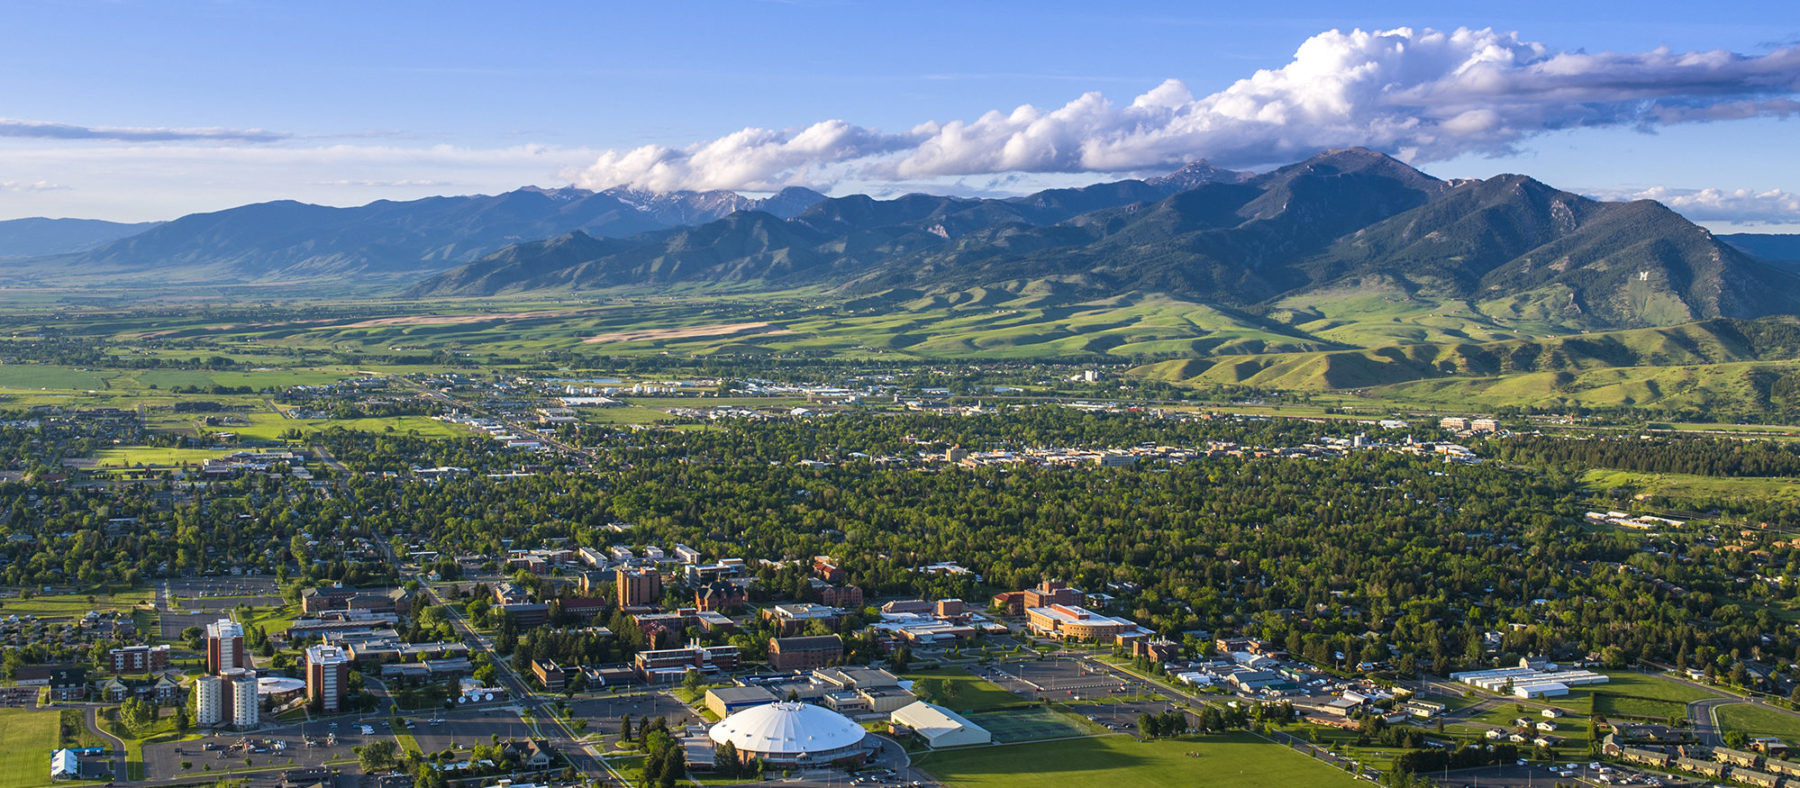
\includegraphics[width=5in,height=\textheight]{images/msu-campus.jpg}}
\usepackage{etoolbox}
\makeatletter
\providecommand{\subtitle}[1]{% add subtitle to \maketitle
  \apptocmd{\@title}{\par {\large #1 \par}}{}{}
}
\makeatother
\subtitle{Fall 2021\\
Montana State University}
\author{Melinda Yager, Jade Schmidt, Dr.~Stacey Hancock}
\date{}

\begin{document}
\maketitle

\newpage
\thispagestyle{empty}

This resource was developed by Melinda Yager, Jade Schmidt, and Stacey Hancock in 2021 to accompany the online textbook: Carnegie, N., Hancock, S., Meyer, E., Schmidt, J., and Yager, M. (2021). \emph{Montana State Introductory Statistics with R}. Montana State University. \url{https://mtstateintrostats.github.io/IntroStatTextbook/}.

This resource is released under a \href{https://creativecommons.org/licenses/by-nc-sa/4.0/}{Creative Commons BY-NC-SA 4.0} license unless otherwise noted.

\setcounter{tocdepth}{1}
\addtocontents{toc}{\protect\thispagestyle{empty}}
\tableofcontents
\thispagestyle{empty}

\newpage
\setcounter{page}{1}

\hypertarget{preface}{%
\chapter*{Preface}\label{preface}}
\addcontentsline{toc}{chapter}{Preface}

This coursepack accompanies the textbook for STAT 216: Introduction to Statistics at Montana State University, which can be found at \url{https://mtstateintrostats.github.io/IntroStatTextbook/}. The syllabus for the course (including the course calendar), data sets, and links to D2L Brightspace, Gradescope, and the MSU RStudio server can be found on the course webpage: \url{https://math.montana.edu/courses/s216/}.
Videos assigned in the course calendar and other notes and review materials are linked in D2L.

Each of the activities in this workbook is designed to target specific learning outcomes of the course, giving you practice with important statistical concepts in a group setting with instructor guidance. In addition to the in-class activities for the course, the coursepack includes reading guides to aid in taking notes while you complete the required readings and videos. Bring this workbook with you to class each class period, and take notes in the workbook as you would your own notes. A well-written completed workbook will provide an optimal study guide for exams!

The activities in this coursepack will be completed during class time on Mondays and Wednesdays. The weekly labs will be completed in class with your group on Fridays. Parts of each lab will be turned in on Gradescope. To aid in your understanding, read through the introduction for each activity before attending class each day.

STAT 216 is a 3-credit in-person course. Students will meet with their instructor and classmates three days per week for 50 minutes. In our experience, it takes six to nine hours per week outside of class to achieve a good grade in this class. By ``good'' we mean at least a C because a grade of D or below does not count toward fulfilling degree requirements. Many of you set your goals higher than just getting a C, and we fully support that. You need roughly nine hours per week to review past activities, read feedback on previous assignments, complete current assignments, and prepare for the next day's class. A typical week in the life of a STAT 216 student looks like:

\begin{itemize}
\tightlist
\item
  \emph{Prior to class meeting}:

  \begin{itemize}
  \tightlist
  \item
    Read assigned sections of the textbook, using the provided reading guides to take notes on the material.
  \item
    Watch assigned videos on that week's content, pausing to take notes and answer video quiz questions.
  \item
    Read through the introduction to the day's in-class activity
  \item
    Read through the week's homework assignment and note any questions you may have on the content.
  \end{itemize}
\item
  \emph{During class meeting}:

  \begin{itemize}
  \tightlist
  \item
    Work through the in-class activity or weekly lab with your classmates and instructor, taking detailed notes on your answers to each question in the activity.
  \end{itemize}
\item
  \emph{After class meeting}:

  \begin{itemize}
  \tightlist
  \item
    Complete any parts of the activity you did not complete in class.
  \item
    Review the posted activity solutions and wrap-up videos, and take notes on key points.
  \item
    Finish watching any remaining assigned videos or readings for the week.
  \item
    Complete the week's homework assignment.
  \end{itemize}
\end{itemize}

\nocite{*}

\hypertarget{fall-2021-calendar-of-in-class-activities}{%
\chapter*{Fall 2021 Calendar of In-Class Activities}\label{fall-2021-calendar-of-in-class-activities}}
\addcontentsline{toc}{chapter}{Fall 2021 Calendar of In-Class Activities}

This calendar only lists the in-class activities, Rstudio labs and exams each week. For required readings and videos as well as due dates for assignments, refer to the calendar at:\\
\href{new\%20calendar}{https://mtstateintrostats.github.io/Syllabus/\#Course\_calendar}

\begin{longtable}{|l|l|l|l|p{.55\textwidth}|}
\hline
\textbf{Week}& \textbf{Day}& \textbf{Date}& \textbf{Activity} \\ \hline
\endhead
1& W& 8/25& Syllabus Review \\*
1& F& 8/27& Martian Alphabet \\ \hline
2& M& 8/30& Atrial Fibrillation \\*
2& W& 9/1& Native American Address \\* 
2& F& 9/3& Week 2 Lab \\ \hline
3& M& 9/6& (\textit{No class}) \\*
3& W& 9/8& What's the Probability? \\*
3& F& 9/10& Week 3 Lab \\ \hline
4& M& 9/13& IMDb Movie Reviews - One Quant Variable \\*
4& W& 9/15& IMDb Movie Reviews - One of Each \\*
4& F& 9/17& Week 4 Lab \\ \hline
5& M& 9/20& Movie Profits - Linear Regression \\*
5& W& 9/22& Movie Profits - Correlation \\* 
5& F& 9/24& Week 5 Lab \\ \hline
6& M& 9/27& Exam 1 Review \\*
6& W& 9/29& Midterm Exam 1 \\*  
6& F& 10/1& Group Midterm Exam 1 \\ \hline
7& M& 10/4& Helper Hinderer --- Simulation HT \\*
7& W& 10/6& Helper Hinderer --- Simulation CI \\*
7& F& 10/8& Week 7 Lab \\ \hline
8& M& 10/11& Handedness of Male Boxers --- Theory HT \\*
8& W& 10/13& Handedness of Male Boxers --- Theory CI \\*    
8& F& 10/15& Week 8 Lab \\ \hline
9& M& 10/18& Good Samaritan --- Simulation HT \\*
9& W& 10/20& Good Samaritan --- Simulation CI \\*   
9& F& 10/22& Week 9 Lab \\ \hline
10& M& 10/25& Helmet Use and Head Injuries --- Theory HT \\*
10& W& 10/27& Helmet Use and Head Injuries --- Theory CI \\*
10& F& 10/29& Week 10 Lab\\ \hline
11& M& 11/1& Exam 2 Review \\*
11& W& 11/3& Midterm Exam 2 \\* 
11& F& 11/5& Group Midterm Exam 2 \\ \hline
12& M& 11/8& COVID and Air Pollution \\*
12& W& 11/10& Construction Costs \\*
12& F& 11/12& Week 12 Lab \\ \hline
13& M& 11/15& Weather Patterns and Snowfall \\*
13& W& 11/17& Homeless Housing Stability \\*
13& F& 11/19& Week 13 Lab \\ \hline
Holiday& M--F& 11/22--11/26& \textbf{No Class --- Fall Break} \\ \hline
14& M& 11/29& Real Estate \\*
14& W& 12/1& Moneyball \\*
14& F& 12/3& Week 14 Lab \\ \hline
15& M& 12/6& Data Exploration \\*
15& W& 12/8& Final Exam Review \\*
15& F& 12/10& Final Exam \\ \hline
Finals& M--W& 12/13--12/15& Final Group Exam \\ \hline

\end{longtable}

\hypertarget{basics-of-data}{%
\chapter{Basics of Data}\label{basics-of-data}}

\hypertarget{reading-guide-basics-of-data}{%
\section{Reading Guide: Basics of Data}\label{reading-guide-basics-of-data}}

\hypertarget{sections-1.1-case-study-and-1.2-data-basics}{%
\subsection*{Sections 1.1 (Case study) and 1.2 (Data basics)}\label{sections-1.1-case-study-and-1.2-data-basics}}
\addcontentsline{toc}{subsection}{Sections 1.1 (Case study) and 1.2 (Data basics)}

\textbf{Videos}

\begin{itemize}
\tightlist
\item
  Stat 216 Course\_Tour
\item
  Instructor bio
\item
  1.2.1\_1.2.2
\item
  1.2.3\_1.2.4\_1.2.5
\end{itemize}

\setstretch{1.25}

\hypertarget{vocabulary}{%
\subsubsection*{Vocabulary}\label{vocabulary}}
\addcontentsline{toc}{subsubsection}{Vocabulary}

Data:
\rgs

Summary statistic:
\rgs

Case/Observational unit:
\rgs

Variable:
\rgs

\rgi Quantitative variable:
\rgs

\rgi Discrete variables:
\rgs

\rgi \rgi Examples of discrete variables using the \texttt{County} data:
\rgs

\rgi Continuous variables:
\rgs

\rgi \rgi Examples of continuous variables using the \texttt{County} data:
\rgs

Example of a number which is NOT a numerical variable:
\rgs

Categorical variable:
\rgs

\rgi Ordinal variable:
\rgs

\rgi \rgi Example of an ordinal variable using the \texttt{County} data:
\rgs

\rgi Nominal variable:
\rgs

\rgi \rgi Examples of nominal variables using the \texttt{County} data:

\rgs

\textbf{Note: Ordinal and nominal variables will be treated the same in this course. We recommend taking more statistics courses in the future to learn better methods of analysis for ordinal variables.}

Data frame:
\rgs

Scatterplot:
\rgs

\rgi Each point represents:

\rgi Positive association:

\rgi Negative association:

Association or Dependent variables:
\rgs

Independent variables:
\rgs

Explanatory variable:
\rgs

Response variable:
\rgs

Observational study:
\rgs

Experiment:
\rgs

Placebo:
\rgs

\hypertarget{notes}{%
\subsubsection*{Notes}\label{notes}}
\addcontentsline{toc}{subsubsection}{Notes}

Big Idea: Variability is inevitable! We would not expect to get \emph{exactly} 50 heads in 100 coin flips. The statistical question then is whether any differences found in data are due to random variability, or if something else is going on.

\begin{quote}
The larger the difference, the \textbf{less we believe the difference was due to chance.}
\end{quote}

In a data frame, rows correspond to \_\_\_\_\_\_\_\_\_\_\_\_\_\_\_\_\_\_\_

and columns correspond to \_\_\_\_\_\_\_\_\_\_\_\_\_\_\_\_\_\_.

How many types of variables are discussed? Explain the differences between them and give an example of each.
\rgs
\rgs

True or False: A pair of variables can be both associated AND independent.\\
True or False: Given a pair of variables, one will always be the explanatory variable and one the response variable.\\
True or False: If a study does have an explanatory and a response variable, that means changes in the explanatory variable must \textbf{cause} changes in the response variable.

True or False: Observational studies can show a naturally occurring association between variables.

\hypertarget{example-section-1.1---case-study-using-stents-to-prevent-strokes}{%
\subsubsection*{Example (Section 1.1 - Case study: Using stents to prevent strokes)}\label{example-section-1.1---case-study-using-stents-to-prevent-strokes}}
\addcontentsline{toc}{subsubsection}{Example (Section 1.1 - Case study: Using stents to prevent strokes)}

\begin{enumerate}
\def\labelenumi{\arabic{enumi}.}
\item
  What is the principle question the researchers hope to answer? (We call this the \textbf{research question}.)
  \rgs
  \rgs
\item
  When creating two groups to compare, do the groups have to be the same size (same number of people in each)?
  \rgs
  \rgs
\item
  What are the cases or observational units in this study?
  \rgs
  \rgs
\item
  Is there a clear explanatory and response variable? If so, name the variable in each role and determine the type of variable (discrete, continuous, nominal, or ordinal).
  \rgs
  \rgs
\item
  What is the purpose of the control group?
  \rgs
  \rgs
\item
  Is this an example of an observational study or an experiment? How do you know?
  \rgs
  \rgs
\item
  Consider Tables 1.1 and 1.2. Which table is more helpful in answering the research question? Justify your answer.
  \rgs
  \rgs
\item
  Describe in words what is shown in Figure 1.1. Specifically, compare the proportion of patients who had a stroke between the treatment and control groups after 30 days as well as after 365 days.
  \rgs
  \rgs
\end{enumerate}

\newpage

\begin{enumerate}
\def\labelenumi{\arabic{enumi}.}
\setcounter{enumi}{8}
\item
  Given the notion that the larger the difference between the two groups (for a given sample size), the less believable it is that the difference was due to chance, which measurement period (30 days or 365 days) provide stronger evidence that there is an association between stents and strokes, or that the differences are not due to random chance?
  \rgs
  \rgs
\item
  This study reported finding evidence that stents \emph{increase} the risk of stroke. Does this conclusion apply to all patients and all stents?
  \rgs
  \rgs
\item
  This study reported finding evidence that stents \emph{increase} the risk of stroke. This conclusion implies a causal link between stents and an increased risk of stroke. Is that conclusion valid? Justify your answer.
\end{enumerate}

\newpage

\hypertarget{activity-1a-martian-alphabet}{%
\section{Activity 1a: Martian Alphabet}\label{activity-1a-martian-alphabet}}

\setstretch{1}

\hypertarget{learning-outcomes}{%
\subsection{Learning outcomes}\label{learning-outcomes}}

\begin{itemize}
\item
  Describe the statistical investigation process.
\item
  Identify observational units, variables, and variable types in a statistical study.
\end{itemize}

\hypertarget{terminology-review}{%
\subsection{Terminology review}\label{terminology-review}}

Statistics is the study of how best to collect, analyze, and draw conclusions from data. Today in class you will be introduced to the following terms:

\begin{itemize}
\item
  Observational units or cases
\item
  Variables: categorical or quantitative
\item
  Proportions
\item
  Graphs: frequency bar plot and relative frequency bar plot
\item
  Distribution
\end{itemize}

For more on these concepts, read Sections 1.2 and 2.1 in the textbook.

\hypertarget{can-you-read-martian}{%
\subsection{Can you read ``Martian?''}\label{can-you-read-martian}}

How well can humans distinguish one ``Martian'' letter from another? In this week's activity, we'll find out. When shown the two Martian letters, Kiki and Bumba, write down whether you think Bumba is on the left or on the right.
\vspace{2mm}

\begin{enumerate}
\def\labelenumi{\arabic{enumi}.}
\tightlist
\item
  Were you correct or incorrect in identifying Bumba?
\end{enumerate}

\vspace{1mm}

\hypertarget{steps-of-the-statistical-investigation-process}{%
\subsubsection*{Steps of the statistical investigation process}\label{steps-of-the-statistical-investigation-process}}
\addcontentsline{toc}{subsubsection}{Steps of the statistical investigation process}

\textbf{Step 1}: The first step of any statistical investigation is to \emph{ask a research question}. In this study the research question is: Can we as a class read Martian? (We will refine this later on!).

\textbf{Step 2}: To answer any research question, we must \emph{design a study and collect data}. For our question, the study consists of each student being presented with two Martian letters and asking which was Bumba. Your responses will become our observed data that we will explore.

\textbf{Observational units} or \textbf{cases} are the subjects data are collected on. In a spreadsheet of the data set, each row will represent a single observational unit.

\begin{enumerate}
\def\labelenumi{\arabic{enumi}.}
\setcounter{enumi}{1}
\tightlist
\item
  What are the observational units in this study?
\end{enumerate}

\vspace{0.2in}

\begin{enumerate}
\def\labelenumi{\arabic{enumi}.}
\setcounter{enumi}{2}
\tightlist
\item
  How many students are in class today? This is the \textbf{sample size}.
\end{enumerate}

\vspace{0.2in}

A \textbf{variable} is information collected or measured on each observational unit or case. Each column in a data set will represent a different variable. Today we are only measuring one variable on each observational unit.

\begin{enumerate}
\def\labelenumi{\arabic{enumi}.}
\setcounter{enumi}{3}
\tightlist
\item
  Identify the variable we are collecting on each observational unit in this study, i.e., what are we measuring on each student? \emph{Hint}: Your answer to question 1 is the outcome for the variable measured on one observational unit.
\end{enumerate}

\vspace{.8in}

We will look at two types of variables: \textbf{quantitative} and \textbf{categorical} (see Figure \ref{fig:types-of-variables}).

Quantitative variables are numerical measurements that can be discrete (whole, non-negative numbers) or continuous (any value within an interval). The number of pets one owns would be a discrete variable as you can not have a partial pet. GPA would be a continuous variable ranging from 0 to 4.0.

The outcome of a categorical variable is a group or category such as eye color, state of residency, or whether or not a student lives on campus. Categorical variables with a natural ordering are considered ordinal variables while those without a natural ordering are considered nominal variables. All categorical variables will be treated as nominal for analysis in this course.

\begin{figure}

{\centering 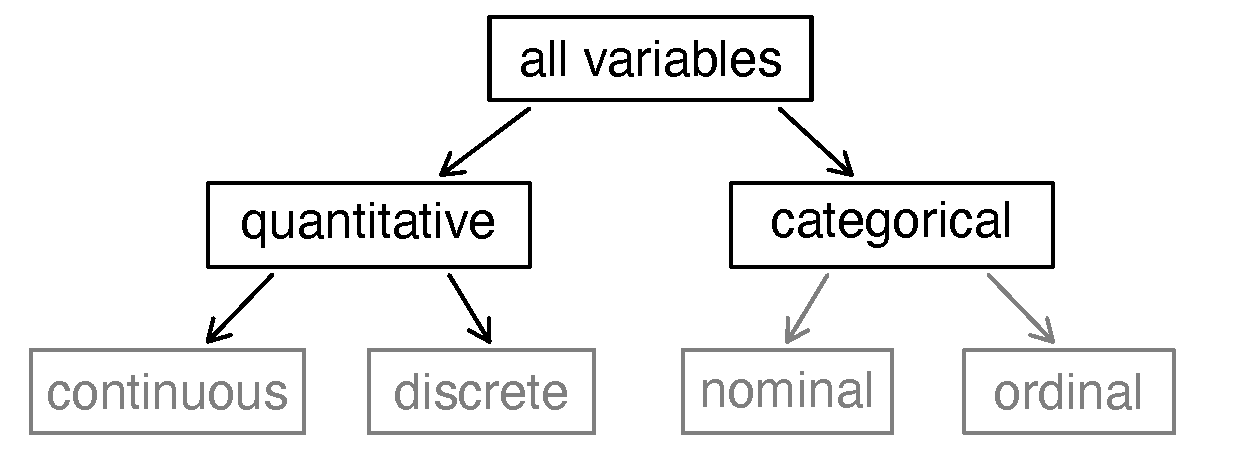
\includegraphics[width=0.5\linewidth]{images/variables} 

}

\caption{Types of variables.}\label{fig:types-of-variables}
\end{figure}

\begin{enumerate}
\def\labelenumi{\arabic{enumi}.}
\setcounter{enumi}{4}
\tightlist
\item
  Is the variable identified in question 4 categorical or quantitative?
\end{enumerate}

\vspace{0.3in}

\textbf{Step 3}: Once we have collected data, the next step is to \emph{summarize and visualize the data}.

\begin{enumerate}
\def\labelenumi{\arabic{enumi}.}
\setcounter{enumi}{5}
\tightlist
\item
  How many people in your class were correct in identifying Bumba? Using the class size from question 3, calculate the proportion of students who correctly identified Bumba.
\end{enumerate}

\begin{center}
$\mbox{proportion} = \frac{\mbox{number of students who correctly identified Bumba}}{\mbox{total number of students}}$
\end{center}

\vspace{0.7in}

The proportion in question 6 is called a \textbf{summary statistic}---a single value that summarizes the data set. It is important to note that a variable is different than a summary statistic. A \emph{variable} is measured on a \emph{single observational unit} while a summary statistic is calculated from a group of observational units. For example, the variable ``whether or not a student lives on campus'' can be measured on each individual student. In a class of 50 students we can calculate the proportion of students who live on campus, the summary statistic. Look back and make sure you wrote the variable in question 4 as a variable, NOT a summary statistic.

Looking at the data set and the summary statistic is only one way to display the data. We will also want to create a visualization or picture of the data. A \textbf{frequency bar plot} is used to display categorical data as a count or frequency. Since our variable has two levels or outcomes, correct or incorrect, we will create two bars---one for each level.

\begin{enumerate}
\def\labelenumi{\arabic{enumi}.}
\setcounter{enumi}{6}
\tightlist
\item
  Plot the observed class data using a frequency bar plot. Be sure to add a scale to the \(y\)-axis.
\end{enumerate}

\begin{center}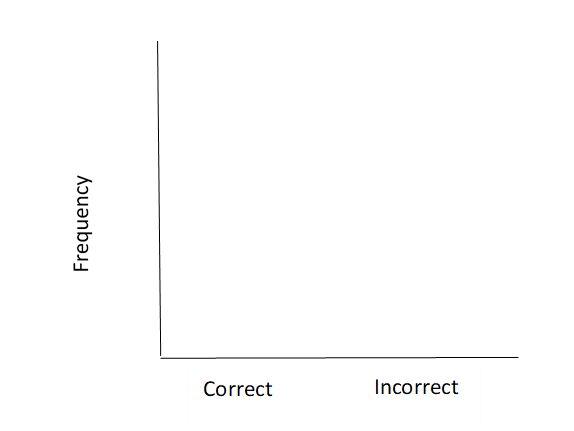
\includegraphics[width=0.4\linewidth]{images/barplot_martian} \end{center}

We can also visualize the data as a proportion in a \textbf{relative frequency bar plot}. Relative frequency is the proportion calculated for each level of the categorical variable.

\begin{enumerate}
\def\labelenumi{\arabic{enumi}.}
\setcounter{enumi}{7}
\tightlist
\item
  Plot the observed class data using a relative frequency bar plot. Be sure to add a scale to the y-axis.
\end{enumerate}

\begin{center}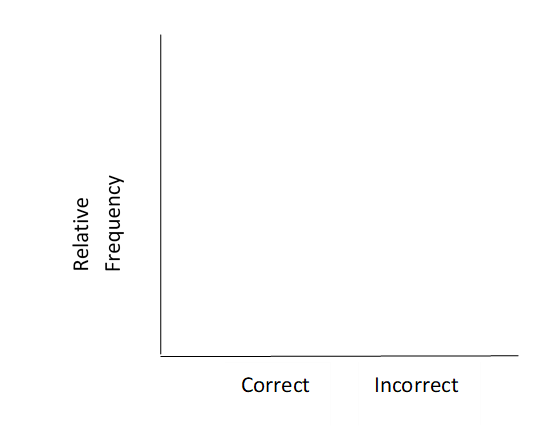
\includegraphics[width=0.4\linewidth]{images/relative_barplot_martian} \end{center}

\textbf{Step 4}: The next step is to \emph{use statistical analysis methods to draw inferences from the data}. To answer the research question, we will simulate what \emph{could} have happened in our class given random chance, repeat many times to understand the expected \emph{variability} between different ``randomly guessing'' classes, then compare our class's observed data to the simulation. This gives us an estimate of how often (or the probability of) the class's result would occur if students were all merely guessing, allowing us to determine if the data provides evidence that we as a class can in fact read Martian.

\begin{enumerate}
\def\labelenumi{\arabic{enumi}.}
\setcounter{enumi}{8}
\item
  If humans really don't know Martian and are just guessing which is Bumba, what are the chances of getting it right?
  \vspace{0.3in}

  How could we use a coin to simulate each student ``just guessing'' which Martian letter is Bumba?
  \vspace{.5in}

  How could we use coins to simulate the entire class ``just guessing'' which Martian letter is Bumba?
  \vspace{.5in}

  How many people in your class would you expect to choose Bumba correctly just by chance? Explain your reasoning.
  \vspace{.5in}
\item
  Each student will flip a coin one time to simulate your ``guess'' under the assumption that we can't read Martian. Let Heads = correct, Tails = incorrect. What was the result of your one simulation?
  \vspace{.3in}

  What was the result from your class's simulation? What proportion of students ``guessed'' correctly in the simulation?
  \vspace{.5in}
\item
  If students really don't know Martian and are just guessing which is Bumba, which seems more unusual: the result from your class's \textbf{simulation} or the observed proportion of students in your class that were correct (this is your summary statistic from question 6)? Explain your reasoning.
\end{enumerate}

\vspace{.8in}

\begin{enumerate}
\def\labelenumi{\arabic{enumi}.}
\setcounter{enumi}{11}
\tightlist
\item
  While your observed class data is likely far different from the simulated ``just-guessing'' class, comparing our class data to a single simulation does not provide enough information. The differences seen could just be due to the randomness of that set of coin flips! Let's simulate another class. Each student should flip their coin again. What was the result from your class's second simulation? What proportion of students ``guessed'' correctly in the second simulation? Create a plot to compare the two simulated results with the observed class result.
\end{enumerate}

\vspace{1.2in}

\begin{enumerate}
\def\labelenumi{\arabic{enumi}.}
\setcounter{enumi}{12}
\tightlist
\item
  We still only have a couple of simulations to compare our class data to. It would be much better to be able to see how our class compared to hundreds or thousands of ``just-guessing'' classes. Since we don't want to flip coins all class period, your instructor will use a computer simulation to get 1000 trials. Fill in the following blanks to describe how we would create a simulation of random guessing with 1000 trials (repetitions).
\end{enumerate}

~~~~~~~~~~Probability of correct guesses: \_\_\_\_\_

\vspace{0.05in}

~~~~~~~~~~Sample size: \_\_\_\_\_

\vspace{0.05in}

~~~~~~~~~~Number of repetitions: \_\_\_\_\_

\vspace{0.05in}

\newpage

\begin{enumerate}
\def\labelenumi{\arabic{enumi}.}
\setcounter{enumi}{13}
\tightlist
\item
  Sketch the distribution displayed by your instructor here. Label each axis appropriately.
\end{enumerate}

\vspace{1.5in}

\begin{enumerate}
\def\labelenumi{\arabic{enumi}.}
\setcounter{enumi}{14}
\tightlist
\item
  Is your class particularly good or bad at Martian? Use the plot in question 14 to explain your answer.
\end{enumerate}

\vspace{.5in}

\begin{enumerate}
\def\labelenumi{\arabic{enumi}.}
\setcounter{enumi}{15}
\tightlist
\item
  Is it \emph{possible} that we could see our class results just by chance if everyone was just guessing? Explain your reasoning.
\end{enumerate}

\vspace{.5in}

\begin{enumerate}
\def\labelenumi{\arabic{enumi}.}
\setcounter{enumi}{16}
\tightlist
\item
  Is it \emph{likely} that we could see our class results just by chance if everyone was just guessing? Explain your reasoning.
\end{enumerate}

\vspace{.5in}

\textbf{Step 5}: The next step in the statistical investigation process is to \emph{communicate the results and answer the research question}.

\begin{enumerate}
\def\labelenumi{\arabic{enumi}.}
\setcounter{enumi}{17}
\tightlist
\item
  Does this activity provide strong evidence that students were not just guessing at random? If so, what do you think is going on here? Can we as a class read Martian?\footnote{Reference for ``Martian alphabet'' is a TED talk given by Vilayanur Ramachandran in 2007. The synesthesia part begins at roughly 17:30 minutes: \texttt{http://www.ted.com/talks/vilayanur\_ramachandran\_on\_your\_mind}.}
\end{enumerate}

\vspace{1in}

\textbf{Step 6}: The final step of any statistical investigation is to \emph{revisit and look ahead}.

\begin{enumerate}
\def\labelenumi{\arabic{enumi}.}
\setcounter{enumi}{18}
\tightlist
\item
  Can you think of any limitations of our study? Can you think of a new topic that might be of interest based on the results of our study?
\end{enumerate}

\vspace{1in}

\newpage

\hypertarget{introduction-to-r}{%
\subsubsection{\texorpdfstring{Introduction to \texttt{R}}{Introduction to R}}\label{introduction-to-r}}

In Stat 216 we will use the statistical package \texttt{R} to analyze data through the IDE (integrated development environment) RStudio. Though it is possible to download \texttt{R} and RStudio on your own computer, we will use this program through the MSU RStudio server: \url{https://rstudio.math.montana.edu/}.

Read through the preliminaries chapter in the textbook and watch the video ``Starting with \texttt{R}'' before completing the following questions.

The RStudio workflow operates best by the use of ``Projects.'' You should create a separate project for each activity or assignment in this course that requires the use of \texttt{R}. To get started with this activity, follow these steps:

\begin{itemize}
\item
  Log onto the RStudio server using your NetID and password: \url{https://rstudio.math.montana.edu/}.

  \begin{itemize}
  \tightlist
  \item
    Please note: Your netID password expires every 6 months. It is HIGHLY recommended that you reset your netID password BEFORE attempting to login to the Rstudio server. You can reset your netID password in the MSU password portal (\url{https://pwreset.montana.edu/react/}).
  \end{itemize}
\item
  In the top right corner, you will see a dropdown menu next to ``Project'' that currently says ``(None).'' Click on this menu and choose ``New Project.'' (Alternatively, you can click the ``File'' menu in the top left and select ``New Project.'')

  \begin{itemize}
  \tightlist
  \item
    A ``New Project Wizard'' window should pop up: click ``New Directory,'' then click ``New Project.''
  \item
    Give your project directory a name (e.g., Activity1). \emph{Do not use spaces or other characters in the name.}
  \item
    Click ``Browse'' and choose a location where you would like to save your project (you can create a new folder if desired). Note that this location is on your server account, not on your computer.
  \item
    Leave all other boxes unchecked, and click ``Create Project.'' (Now, if you click on the home icon in the top right, you will see your RStudio account, and the project should be listed under ``Projects.'')
  \end{itemize}
\item
  Download the Martian Alphabet \texttt{R} script file from D2L.
\item
  Click ``Upload'' in the ``Files'' tab in the bottom right window of RStudio. Click ``Choose File,'' and navigate to the folder where the Martian Alphabet \texttt{R} script file is saved. Then click ``Open''; then click ``Ok.''
\item
  You should see the uploaded file appear in the list of files. Click on the filename to open the file.
\end{itemize}

In the Martian Alphabet \texttt{R} script file, highlight the lines of code that starts with \texttt{library} and click ``Run.'' This will load the \textbf{package} (or library) \texttt{catstats} needed for this activity; each package is a collection of \texttt{R} functions. We review a few of these packages here.

\begin{itemize}
\tightlist
\item
  Throughout the semester we will use the package \texttt{tidyverse} to allow us to use chaining (see Section 1.7 in the textbook for more on this symbol \texttt{\%\textgreater{}\%}.) Contained in \texttt{tidyverse} is the package \texttt{ggplot2}, used to create graphs in RStudio.
\item
  The package \texttt{mosaic} contains the \texttt{favstats()} function to find summary statistics for quantitative variables.
\item
  We will use the package \texttt{catstats}, starting in Chapter 5 (and in this activity), to create simulations for statistical inference.
\end{itemize}

These packages are already installed in the RStudio server, but you need to use the \texttt{library()} function to call the package into your R environment. We will only use the package \texttt{catstats} for this activity.

The \# sign is not part of the \texttt{R} code.
It is used by these authors to add comments to the \texttt{R} code and explain what each call is telling the program to do.
\texttt{R} will ignore everything after a \# sign when executing the code.

In the Martian Alphabet \texttt{R} script file for the \texttt{one\_proportion\_test()} function arguments, enter your class size (Q3 from the in-class activity) for \texttt{sample\_size} and the number of students who were correct in identifying Bumba (Q6 from the in-class activity) for \texttt{as\_extreme\_as} argument. Highlight lines 3 -- 8 and click run.

Is the distribution created from this code similar to what you saw in class in Q14?

\vspace{0.3in}

\hypertarget{take-home-messages}{%
\subsection{Take-home messages}\label{take-home-messages}}

\begin{enumerate}
\def\labelenumi{\arabic{enumi}.}
\item
  In this course we will learn how to evaluate a claim by comparing observed results (classes' ``guesses'' when asked to identify Bumba) to a distribution of many simulated results under an assumption like ``blind guessing.''
\item
  Blind guessing between two outcomes will be correct only about half the time. We can simulate data using a computer program to fit the assumption of blind guessing.
\item
  Unusual observed results will make us doubt the assumptions used to create the simulated distribution. A large number of correct ``guesses'' is evidence that a person was not just blindly guessing.
\end{enumerate}

\hypertarget{additional-notes}{%
\subsection{Additional notes}\label{additional-notes}}

Use this space to summarize your thoughts and take additional notes on today's activity and material covered, and to write down the names and contact information of your teammates.

\hypertarget{study-design}{%
\chapter{Study Design}\label{study-design}}

\hypertarget{week-2---reading-guide-sampling-experimental-design-and-scope-of-inference}{%
\section{Week 2 - Reading Guide: Sampling, Experimental Design, and Scope of Inference}\label{week-2---reading-guide-sampling-experimental-design-and-scope-of-inference}}

\hypertarget{section-1.3-sampling-principles-and-strategies}{%
\subsection*{Section 1.3 (Sampling principles and strategies)}\label{section-1.3-sampling-principles-and-strategies}}
\addcontentsline{toc}{subsection}{Section 1.3 (Sampling principles and strategies)}

\textbf{Videos}

\begin{itemize}
\tightlist
\item
  1.3
\end{itemize}

\setstretch{1.25}

\hypertarget{vocabulary-1}{%
\subsubsection*{Vocabulary}\label{vocabulary-1}}
\addcontentsline{toc}{subsubsection}{Vocabulary}

(Target) Population:
\rgs

Sample:
\rgs

Anecdotal evidence:
\rgs

Bias:
\rgs

\rgi Selection bias:
\rgs

\rgi Non-response bias:
\rgs

\rgi Response bias:
\rgs

Convenience sample:
\rgs

Simple Random Sample:
\rgs

Non-response rate:
\rgs

Representative:
\rgs

\hypertarget{notes-1}{%
\subsubsection*{Notes}\label{notes-1}}
\addcontentsline{toc}{subsubsection}{Notes}

Ideally, how should we sample cases from our target population? Using what sampling method?
\rgs

\hypertarget{notes-on-types-of-sampling-bias}{%
\paragraph*{Notes on types of sampling bias}\label{notes-on-types-of-sampling-bias}}
\addcontentsline{toc}{paragraph}{Notes on types of sampling bias}

\begin{itemize}
\item
  Someone must first be \emph{chosen} to be in a study and refuse to participate in order to have \textbf{non-response bias}.
\item
  There must be a valid reason for someone to lie or be untruthful to justify saying \textbf{response bias} is present. Yes, anyone could lie at any time to any question. Response bias is when those lies are predictable and systematic based on outside influences.
  \rgs
\end{itemize}

True or False: Convenience sampling tends to result in non-response bias.

True or False: Volunteer sampling tends to result in response bias.

True or False: Random sampling helps to resolve selection bias, but has no impact on non-response or response bias.

\hypertarget{sections-1.4-observational-studies-1.5-experiments-and-1.6-scope-of-inference}{%
\subsection*{Sections 1.4 (Observational studies), 1.5 (Experiments), and 1.6 (Scope of inference)}\label{sections-1.4-observational-studies-1.5-experiments-and-1.6-scope-of-inference}}
\addcontentsline{toc}{subsection}{Sections 1.4 (Observational studies), 1.5 (Experiments), and 1.6 (Scope of inference)}

\setstretch{1}

\textbf{Videos}

\begin{itemize}
\tightlist
\item
  1.4to1.6
\end{itemize}

\setstretch{1.25}

\hypertarget{reminders-from-section-1.2}{%
\subsubsection*{Reminders from Section 1.2}\label{reminders-from-section-1.2}}
\addcontentsline{toc}{subsubsection}{Reminders from Section 1.2}

\textbf{Explanatory variable}: The variable researchers think \emph{may be} affecting the other variable. What the researchers control/assign in an experiment. If comparing groups, the explanatory variable puts the observational units into groups.

\textbf{Response variable}: The variable researchers think \emph{may be} influenced by the other variable. This variable is always observed, never controlled or assigned.

\hypertarget{vocabulary-2}{%
\subsubsection*{Vocabulary}\label{vocabulary-2}}
\addcontentsline{toc}{subsubsection}{Vocabulary}

Observational study:
\rgs

\rgi Observational data:
\rgs

\rgi Prospective study:
\rgs

\rgi Retrospective study:
\rgs

Confounding variable:
\rgs

Experiment:
\rgs

\rgi Randomized experiment:
\rgs

\rgi Blocking:
\rgs

\rgi Treatment group:
\rgs

\rgi Control group:
\rgs

\rgi Placebo:
\rgs

\rgi Placebo effect:
\rgs

\rgi Blinding:
\rgs

Scope of inference:
\rgs

Generalizability:
\rgs

Causation:
\rgs

\hypertarget{notes-2}{%
\subsubsection*{Notes}\label{notes-2}}
\addcontentsline{toc}{subsubsection}{Notes}

What are the four principles of a well-designed randomized experiment?\\
\rgs
\rgs
\rgs

Fill in the appropriate scope of inference for each study design.

\begin{center}
\begin{tabular}{|p{2in}|p{2in}|p{2in}|}
\hline
 & \multicolumn{2}{|c|}{\textbf{Study Type}} \\ \hline
 \textbf{Selection of Cases} & Randomized experiment & Observational study \\ \hline
 Random sample && \\ 
 (and no other sampling bias) & & \\ 
  & & \\
   & & \\ \hline
   Non-random sample && \\ 
   (or other sampling bias) & & \\ 
  & & \\
   & & \\ \hline
\end{tabular}
\end{center}

\rgs

True or False: Observational studies can show an association between two variables, but cannot determine a causal relationship.

True or False: In order for an experiment to be valid, a placebo must be used.

True or False: If random sampling of the target population is used, and no other types of bias are suspected, results from the sample can be generalized to the entire target population.

True or False: If random sampling of the target population is used, and no other types of bias are suspected, results from the sample can be inferred as a causal relationship between the explanatory and response variables.

\newpage

\hypertarget{activity-2a-atrial-fibrillation-study-design}{%
\section{Activity 2a: Atrial Fibrillation (Study Design)}\label{activity-2a-atrial-fibrillation-study-design}}

\setstretch{1}

\hypertarget{learning-outcomes-1}{%
\subsection{Learning outcomes}\label{learning-outcomes-1}}

\begin{itemize}
\item
  Explain the purpose of random assignment and its effect on scope of inference.
\item
  Identify whether a study design is observational or an experiment.
\item
  Identify confounding variables in observational studies and explain why they are confounding.
\end{itemize}

\hypertarget{terminology-review-1}{%
\subsection{Terminology review}\label{terminology-review-1}}

In this activity, we will examine different study designs, confounding variables, and how to determine the scope of inference for a study. Some terms covered in this activity are:

\begin{itemize}
\item
  Scope of inference
\item
  Explanatory variable
\item
  Response variable
\item
  Confounding variable
\item
  Experiment
\item
  Observational study
\end{itemize}

To review these concepts, see Sections 1.3 through 1.6 in the textbook.

\hypertarget{study-design-1}{%
\subsection{Study design}\label{study-design-1}}

The two main study designs we will cover are \textbf{observational studies} and \textbf{experiments}. Both the sampling method (which we will cover in next class) and the study design will help to determine the \textbf{scope of inference} for a study: To \emph{whom}\_\_ can we generalize, and can we conclude causation or only association? Remember that only in a randomized experiment can we conclude a \textbf{causal} (cause and effect) relationship between the explanatory and response variable.

\begin{center}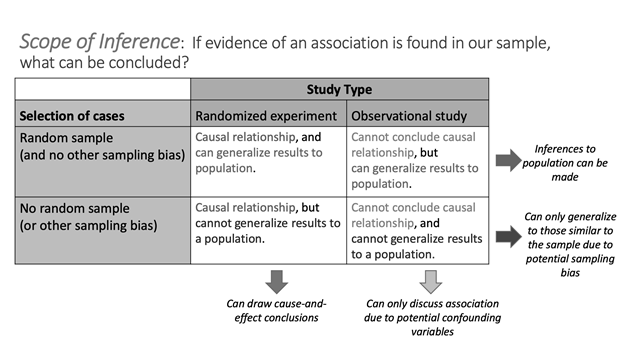
\includegraphics[width=0.75\linewidth]{images/ScopeOfInferenceGreyscale} \end{center}

\hypertarget{take-home-messages-1}{%
\subsection{Take-home messages}\label{take-home-messages-1}}

\begin{enumerate}
\def\labelenumi{\arabic{enumi}.}
\item
  The study design determines if we can draw causal inferences or not. If an association is detected, a randomized experiment allows us to conclude that there is a causal (cause-and-effect) relationship between the explanatory and response variable. Observational studies have potential confounding variables within the study that prevent us from inferring a causal relationship between the variables.
\item
  Confounding variables are variables not included in the study that are related to both the explanatory and the response variables. When there are potential confounding variables in the study we cannot draw causal inferences.
\end{enumerate}

\hypertarget{additional-notes-1}{%
\subsection{Additional notes}\label{additional-notes-1}}

Use this space to summarize your thoughts and take additional notes on today's activity and material covered.

\newpage

\hypertarget{activity-2b-native-american-address}{%
\section{Activity 2b: Native American Address}\label{activity-2b-native-american-address}}

\setstretch{1}

\hypertarget{learning-outcomes-2}{%
\subsection{Learning outcomes}\label{learning-outcomes-2}}

\begin{itemize}
\item
  Explain the purpose of random selection and its effect on scope of inference.
\item
  Select a simple random sample from a finite population using a random number generator.
\item
  Explain why a sampling method is unbiased or biased.
\end{itemize}

\hypertarget{terminology-review-2}{%
\subsection{Terminology review}\label{terminology-review-2}}

In today's activity, we will examine unbiased and biased methods of sampling. Some terms covered in this activity are:

\begin{itemize}
\item
  Random sample
\item
  Unbiased vs biased methods of selection
\item
  Generalization
\end{itemize}

To review these concepts, see Sections 1.3 through 1.6 in the textbook.

\hypertarget{native-american-address}{%
\subsection{Native American Address}\label{native-american-address}}

For this activity, you will read a speech given by Jim Becenti, a member of the Navajo American Indian tribe, who spoke about the employment problems his people faced at an Office of Indian Affairs meeting in Phoenix, Arizona, on January 30, 1947. His speech is below:

\textbf{It is hard for us to go outside the reservation where we meet strangers. I have been off the reservation ever since I was sixteen. Today I am sorry I quit the Santa Fe {[}Railroad{]}. I worked for them in 1912-13. You are enjoying life, liberty, and happiness on the soil the American Indian had, so it is your responsibility to give us a hand, brother. Take us out of distress. I have never been to vocational school. I have very little education. I look at the white man who is a skilled laborer. When I was a young man I worked for a man in Gallup as a carpenter's helper. He treated me as his own brother. I used his tools. Then he took his tools and gave me a list of tools I should buy and I started carpentering just from what I had seen. We have no alphabetical language. We see things with our eyes and can always remember it. I urge that we help my people to progress in skilled labor as well as common labor. The hope of my people is to change our ways and means in certain directions, so they can help you someday as taxpayers. If not, as you are going now, you will be burdened the rest of your life. The hope of my people is that you will continue to help so that we will be all over the United States and have a hand with you, and give us a brotherly hand so we will be happy as you are. Our reservation is awful small. We did not know the capacity of the range until the white man come and say ``you raise too much sheep, got to go somewhere else,'' resulting in reduction to a skeleton where the Indians can't make a living on it. For eighty years we have been confused by the general public, and what is the condition of the Navajo today? Starvation! We are starving for education. Education is the main thing and the only thing that is going to make us able to compete with you great men here talking to us.}

\hypertarget{by-eye-selection}{%
\subsubsection*{By eye selection}\label{by-eye-selection}}
\addcontentsline{toc}{subsubsection}{By eye selection}

\begin{enumerate}
\def\labelenumi{\arabic{enumi}.}
\tightlist
\item
  Circle ten words in Jim Becenti's speech which are a representative sample of the entire text. Describe your method for selecting this sample.
\end{enumerate}

\vspace{0.5in}

\begin{enumerate}
\def\labelenumi{\arabic{enumi}.}
\setcounter{enumi}{1}
\tightlist
\item
  Fill in the table below with your selected words from the preview assignment and the length of each word (number of letters/digits in the word):
  \vspace{1mm}
\end{enumerate}

\begin{figure}

{\centering 
\includegraphics[width=0.5\linewidth]{images/word_length} 

}

\end{figure}

\begin{enumerate}
\def\labelenumi{\arabic{enumi}.}
\setcounter{enumi}{2}
\item
  Calculate the mean word length in your selected sample. Is this value a parameter or a statistic?\\
  \vspace{0.3in}
\item
  Report your mean word length to your instructor. Your instructor will guide the class in creating a visualization of the distribution results generated by your class. Draw a picture of the plot here. Include a descriptive x-axis label.
  \vspace{1.5in}
\item
  Based on the plot of sample mean word lengths in question 4, what is your best guess for the average word length of the population of all 359 words in the speech?
  \vspace{0.3in}
\end{enumerate}

\newpage

\begin{enumerate}
\def\labelenumi{\arabic{enumi}.}
\setcounter{enumi}{5}
\tightlist
\item
  The true mean word length of the population of all 359 words in the speech is 3.95 letters. Is this value a parameter or a statistic?\\
  \vspace{0.2in}
\end{enumerate}

\rgi Where does the value of 3.95 fall in our plot above?
\vspace{0.3in}

\begin{enumerate}
\def\labelenumi{\arabic{enumi}.}
\setcounter{enumi}{6}
\item
  If your samples were truly representative, what proportion of sample means would you expect to be above 3.95?
  \vspace{0.5in}
\item
  What proportion of students' computed sample means were larger than the true mean of 3.95 letters?
  \vspace{0.5in}
\end{enumerate}

\hypertarget{random-selection}{%
\subsubsection*{Random selection}\label{random-selection}}
\addcontentsline{toc}{subsubsection}{Random selection}

Suppose instead of selecting a representative sample by eye, each student used a random number generator to select a simple random sample of 10 words. A simple random sample relies on a random mechanism to choose a sample, without replacement, from the population, such that every sample of size 10 is equally likely to be chosen.

To use a random number generator to select a simple random sample, you first need a numbered list of all the words in the population, called a sampling frame. You can then generate 10 random numbers from the numbers 1 to 359 (the number of words in the population), and the chosen random numbers correspond to the chosen words in your sample.

\begin{enumerate}
\def\labelenumi{\arabic{enumi}.}
\setcounter{enumi}{8}
\tightlist
\item
  Use the random number generator at \url{https://istats.shinyapps.io/RandomNumbers/} and the sampling frame provided to select a simple random sample from the population of all 359 words in the speech. Fill in the table below with the random numbers selected and each number's corresponding word and word length (number of letters/digits in the word):
\end{enumerate}

\begin{figure}

{\centering 
\includegraphics[width=0.5\linewidth]{images/random_word_length} 

}

\end{figure}

\begin{enumerate}
\def\labelenumi{\arabic{enumi}.}
\setcounter{enumi}{9}
\item
  Calculate the mean word length in your selected sample in question 9. Is this value a parameter or a statistic?
  \vspace{0.3in}
\item
  Report your mean word length to your instructor. Your instructor will guide the class in creating a visualization of the distribution results generated by your class. Draw a picture of the plot here. Include a descriptive x-axis label.
  \vspace{1.5in}
\item
  Where does the value 3.95, the true mean word length, fall in the distribution created in question 11?
  \vspace{0.3in}
\item
  How does the plot generated in question 11 compare to the plot generated in question 5?
\end{enumerate}

\rgi Which features are similar?\\
\vspace{0.4in}

\rgi Which features differ?

\vspace{0.4in}

\rgi Why didn't everyone get the same sample mean?
\vspace{0.4in}
\newpage

\begin{enumerate}
\def\labelenumi{\arabic{enumi}.}
\setcounter{enumi}{13}
\tightlist
\item
  One set of randomly generated sample mean word lengths from a single class may not be large enough to visualize the distribution results. Let's have a computer generate 1,000 sample mean word lengths for us.
\end{enumerate}

\begin{itemize}
\item
  Navigate to the ``Sampling Distribution of the Sample Mean (Continuous Population)'' Art of Stat web applet: \url{https://istats.shinyapps.io/sampdist_cont/}.
\item
  Under ``Select Population Distribution,'' select ``Build Your Own.''
\item
  Copy and paste the population of word lengths into the applet from the data set provided. \textbf{Only copy column 3 with NO header}.
\item
  Select 10 for the sample size.
\item
  Select 1,000 for the number of samples to simulate drawing from the population.
\item
  Click ``Draw Sample(s).''
\end{itemize}

The plot labeled ``Sampling Distribution of the Sample Mean'' displays the 1,000 randomly generated sample mean word lengths. Sketch this plot below.
\vspace{1.5in}

\begin{enumerate}
\def\labelenumi{\arabic{enumi}.}
\setcounter{enumi}{14}
\item
  What is the center value of this distribution created in question 14?
  \vspace{0.3in}
\item
  Explain why the sampling method of using a random number generator to generate a sample is a ``better'' method than choosing 10 words ``by eye.''
  \vspace{0.8in}
\item
  Which method of selection, ``by eye'' or random selection, is an unbiased method of selection?
  \vspace{0.5in}
\item
  Explain why the human sampling method of choosing 10 words by eye is biased? What is the direction of the bias, i.e., does the method tend to overestimate or underestimate the population mean word length?
  \vspace{0.8in}
\end{enumerate}

\hypertarget{take-home-messages-2}{%
\subsection{Take-home messages}\label{take-home-messages-2}}

\begin{enumerate}
\def\labelenumi{\arabic{enumi}.}
\item
  When we use a biased method of selection, we will over or underestimate the population mean.
\item
  Random selection is an unbiased method of selection.
\item
  To see if a method is biased, we compare the distribution of the estimates
  to the true value. We want our estimate to be on target or unbiased. When using unbiased methods of selection, the mean of the distribution matches our true parameter.
\item
  If the sampling method is biased, inferences made about the population based on a sample estimate will not be valid. Random sampling avoids this problem.
\end{enumerate}

\hypertarget{additional-notes-2}{%
\subsection{Additional notes}\label{additional-notes-2}}

Use this space to summarize your thoughts and take additional notes on today's activity and material covered.

\newpage

\hypertarget{week-2-lab-study-design}{%
\section{Week 2 Lab: Study Design}\label{week-2-lab-study-design}}

\setstretch{1}

\hypertarget{learning-outcomes-3}{%
\subsection{Learning outcomes}\label{learning-outcomes-3}}

\begin{itemize}
\item
  Explain the purpose of random assignment and its effect on scope of inference.
\item
  Identify whether a study design is observational or an experiment.
\item
  Identify confounding variables in observational studies and explain why they are confounding.
\item
  Explain the effect of sample size on sampling variability
\end{itemize}

\hypertarget{terminology-review-3}{%
\subsection{Terminology review}\label{terminology-review-3}}

In this week's lab, we will examine different types of sampling bias and study designs, confounding variables, and how to determine the scope of inference for a study. Some terms covered in this activity are:

\begin{itemize}
\item
  Scope of inference
\item
  Explanatory variable
\item
  Response variable
\item
  Confounding variable
\item
  Experiment
\item
  Observational study
\item
  Types of sampling bias
\end{itemize}

To review these concepts, see Sections 1.3 through 1.6 in the textbook.

\hypertarget{study-design-2}{%
\subsection{Study Design}\label{study-design-2}}

Each Friday you will complete a lab in class with your group. Questions are selected from each lab to be turned in on Gradescope (one submission per group). The questions to be submitted on Gradescope are bolded in the lab. As you work through the lab with your group have the Gradescope lab assignment open so that you can answer those questions as you go.

\hypertarget{types-of-sampling-bias.}{%
\subsection*{Types of sampling bias.}\label{types-of-sampling-bias.}}
\addcontentsline{toc}{subsection}{Types of sampling bias.}

In today's activity, we will look at sampling and types of bias (selection, non-response, or response).

In these next questions, identify the target population, the sample selected, the variable, and the type of bias present.

\begin{enumerate}
\def\labelenumi{\arabic{enumi}.}
\item
  To determine if the proportion of out-of-state undergraduate students at Montana State University has increased in the last 10 years, a statistics instructor sent an email survey to 500 randomly selected current undergraduate students. One of the questions on the survey asked whether they had in-state or out-of-state residency. She only received 378 responses.
  \vspace{0.25in}

  Target population:
  \vspace{0.3in}

  Sample:
  \vspace{0.3in}

  Variable:
  \vspace{0.3in}

  Type(s) of bias:
  \vspace{0.3in}
\item
  A television station is interested in predicting whether or not a local referendum to legalize marijuana for adult use will pass. It asks its viewers to phone in and indicate whether they are in favor or opposed to the referendum. Of the 2241 viewers who phoned in, forty-five percent were opposed to legalizing marijuana.
  \vspace{0.1in}

  Target population:
  \vspace{0.3in}

  Sample:
  \vspace{0.3in}

  Variable:
  \vspace{0.3in}

  Type(s) of bias:
  \vspace{0.3in}
\item
  To gauge the interest in a new swimming pool, a local organization stood outside of the Bogart Pool in Bozeman, MT, during open hours. One of the questions they asked was, ``Since the Bogart Pool is in such bad repair, don't you agree that the city should fund a new pool?''
  \vspace{0.1in}

  Target population:
  \vspace{0.3in}

  Sample:
  \vspace{0.3in}

  Variable:
  \vspace{0.3in}

  Type(s) of bias:
  \vspace{0.3in}
\item
  The Bozeman school district is interested in surveying parents of students about their opinions on returning to in-person classes following the COVID-19 pandemic. They divided the school district into 10 divisions based on location and randomly surveyed 20 households within each division. Explain why selection bias would be present in this study design.
  \vspace{1in}
\item
  What is the purpose of random selection of a sample from the population?
\end{enumerate}

\vspace{0.8in}

\hypertarget{scope-of-inference}{%
\subsection*{Scope of inference}\label{scope-of-inference}}
\addcontentsline{toc}{subsection}{Scope of inference}

For the next exercises, identify the explanatory variable, the response variable, the study design (observational study or experiment), and the scope of inference (using the following chart).

\begin{center}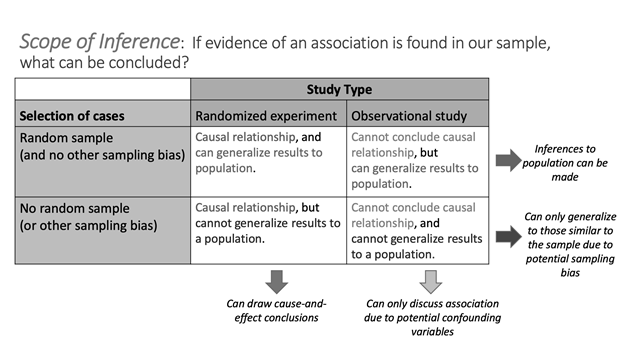
\includegraphics[width=0.75\linewidth]{images/ScopeOfInferenceGreyscale} \end{center}

\begin{enumerate}
\def\labelenumi{\arabic{enumi}.}
\setcounter{enumi}{5}
\item
  The pharmaceutical company Moderna Therapeutics, working in conjunction with the National Institutes of Health, conducted Phase 3 clinical trials towards a vaccine for COVID-19 last fall. US clinical research sites enrolled 30,000 volunteers without COVID-19 to participate. Participants were randomly assigned to receive either the candidate vaccine or a saline placebo. They were then followed to assess whether or not they developed COVID-19. The trial was double-blind, so neither the investigators nor the participants knew who was assigned to which group.
  \vspace{0.1in}

  Explanatory variable:
  \vspace{0.25in}

  Response variable:
  \vspace{0.25in}

  Study design:
  \vspace{0.25in}

  What is the scope of inference for this study?
  \vspace{0.5in}
\end{enumerate}

\newpage

\begin{enumerate}
\def\labelenumi{\arabic{enumi}.}
\setcounter{enumi}{6}
\item
  In another study, a local health department randomly selected 1000 US adults without COVID-19 to participate in a health survey. Each participant was assessed at the beginning of the study and then followed for one year. They were interested to see which participants elected to receive a vaccination for COVID-19 and whether any participants developed COVID-19.
  \vspace{0.1in}

  Explanatory variable:
  \vspace{0.25in}

  Response variable:
  \vspace{0.25in}

  Study design:
  \vspace{0.25in}

  What is the scope of inference for this study?
  \vspace{0.5in}
\end{enumerate}

A \textbf{confounding variable} is a variable that is \emph{both}

\begin{enumerate}
\def\labelenumi{\arabic{enumi}.}
\tightlist
\item
  associated with the explanatory variable, \emph{and}
\item
  associated with the response variable.
\end{enumerate}

When both these conditions are met, if we observe an association between the explanatory variable and the response variable in the data, we cannot be sure if this association is due to the explanatory variable or the confounding variable---the explanatory and confounding variables are ``confounded.''

\begin{center}\includegraphics[width=0.4\linewidth]{02-L01-study-design_files/figure-latex/unnamed-chunk-2-1} \end{center}

\begin{enumerate}
\def\labelenumi{\arabic{enumi}.}
\setcounter{enumi}{7}
\item
  For each of the studies in questions 6 and 7, determine whether confounding variables could be an issue. If so, identify a potential confounding variable and explain how it meets the definition of a confounding variable.
  \vspace{1.5in}
\item
  A study published in 2007 by Christopher Johnson, professor of music education and music therapy at the University of Kansas, revealed that students in elementary schools with superior music education programs scored around 20 percent higher in math scores on standardized tests, compared to schools with low-quality music programs. Explain how school budget could be a potential confounding variable. Be sure to address how the confounding variable is related to both the explanatory and response variable.
\end{enumerate}

\vspace{1in}

\begin{enumerate}
\def\labelenumi{\arabic{enumi}.}
\setcounter{enumi}{9}
\tightlist
\item
  What is the purpose of random assignment of the cases in a study to the explanatory variable groups?
\end{enumerate}

\vspace{0.8in}

\hypertarget{effect-of-sample-size}{%
\subsection*{Effect of sample size}\label{effect-of-sample-size}}
\addcontentsline{toc}{subsection}{Effect of sample size}

\begin{enumerate}
\def\labelenumi{\arabic{enumi}.}
\setcounter{enumi}{10}
\tightlist
\item
  Let's return to the Native American Address study. In today's activity we will select 20 words instead of 10 words at random.
\end{enumerate}

\begin{itemize}
\item
  Navigate to the ``Sampling Distribution of the Sample Mean (Continuous Population)'' Art of Stat web applet: \url{https://istats.shinyapps.io/sampdist_cont/}.
\item
  Under ``Select Population Distribution,'' select ``Build Your Own.''
\item
  Copy and paste the population of word lengths into the applet from the data set provided. \textbf{Only copy column 3 with NO header}.
\item
  Select 20 for the sample size.
\item
  Select 1,000 for the number of samples to simulate drawing from the population.
\item
  Click ``Draw Sample(s).''
\end{itemize}

The plot labeled ``Sampling Distribution of the Sample Mean'' displays the 1,000 randomly generated sample mean word lengths. Sketch this plot below.
\vspace{1.5in}

\newpage

\begin{enumerate}
\def\labelenumi{\arabic{enumi}.}
\setcounter{enumi}{11}
\tightlist
\item
  Compare the distribution created in question 11 to the one created in question 14 in Activity 2a.
\end{enumerate}

\rgi Which features are similar?\\
\vspace{0.4in}

\rgi Which features differ?

\vspace{0.4in}

\begin{enumerate}
\def\labelenumi{\arabic{enumi}.}
\setcounter{enumi}{12}
\item
  Compare the spreads of the plots in question 11 and in question 14 in Activity 2a. You should see that in one plot all sample means are closer to the population mean than in the other. Which plot shows this?
  \vspace{0.4in}
\item
  Using the evidence from your simulations, answer the following research questions.
\end{enumerate}

\rgi Does changing the sample size impact whether the sample estimates are unbiased? Explain your answer.
\vspace{0.5in}

\rgi Does changing the sample size impact the variability of sample estimates? Explain your answer
\vspace{0.5in}

\hypertarget{exploring-categorical-data}{%
\chapter{Exploring Categorical Data}\label{exploring-categorical-data}}

\hypertarget{week-3---reading-guide-introduction-to-r-categorical-data-and-probability}{%
\section{\texorpdfstring{Week 3 - Reading Guide: Introduction to \texttt{R}, Categorical Data, and Probability}{Week 3 - Reading Guide: Introduction to R, Categorical Data, and Probability}}\label{week-3---reading-guide-introduction-to-r-categorical-data-and-probability}}

\hypertarget{section-1.7-data-in-r}{%
\subsection*{\texorpdfstring{Section 1.7 (Data in \texttt{R})}{Section 1.7 (Data in R)}}\label{section-1.7-data-in-r}}
\addcontentsline{toc}{subsection}{Section 1.7 (Data in \texttt{R})}

\textbf{Videos}

\begin{itemize}
\tightlist
\item
  Starting\_with\_R
\end{itemize}

\setstretch{1.25}

\hypertarget{notes-3}{%
\subsubsection*{Notes}\label{notes-3}}
\addcontentsline{toc}{subsubsection}{Notes}

\texttt{R} is case sensitive, meaning it reads \texttt{data} differently from \texttt{Data}. If you get an error message, check that your capitalization is correct.

\texttt{R} does not like spaces or special characters This means the column and row headers in the data set should not have spaces, periods, commas, etc. Instead of titling the variable \texttt{column\ header}, use \texttt{column\_header} or \texttt{ColumnHeader}.

\textbf{Tidy data}: Data frames with

\rgi 1 row per \_\_\_\_\_\_\_\_\_\_\_\_\_\_\_\_,

\rgi 1 column per \_\_\_\_\_\_\_\_\_\_\_\_.

We highly recommend completing Tutorial 1 at the end of Chapter 1 (all four lessons) to give you practice with R/RStudio AND to help reflect on the content of Chapter 1: basics of data, sampling, study design, and scope of inference. These tutorials have some content questions and some places for you to practice using R online with some guidance.

\rgi \_\_ indicate spots you need to type in functions, data sets, or variable names.

\rgi There are Hint and Solution buttons on the R code box to help you.

We would not expect you to know the coding right now, especially for things like mutations or creating new variables in the data set. But seeing some initial coding for these more difficult functions will only make you more comfortable using the functions needed for this course!

\hypertarget{functions}{%
\subsubsection*{Functions}\label{functions}}
\addcontentsline{toc}{subsubsection}{Functions}

State what these introductory functions do in \texttt{R}:

\texttt{glimpse(data\_set\_name)}

\texttt{head(data\_set\_name)}

\texttt{data\_set\_name\$variable\_name}

\texttt{\%\textgreater{}\%}

\texttt{\textless{}-}

\hypertarget{section-2.1-exploring-categorical-data}{%
\subsection*{Section 2.1 (Exploring categorical data)}\label{section-2.1-exploring-categorical-data}}
\addcontentsline{toc}{subsection}{Section 2.1 (Exploring categorical data)}

\setstretch{1}

\textbf{Videos}

\begin{itemize}
\tightlist
\item
  2.1
\item
  MosaicPlots
\end{itemize}

\setstretch{1.25}

\hypertarget{vocabulary-3}{%
\subsubsection*{Vocabulary}\label{vocabulary-3}}
\addcontentsline{toc}{subsubsection}{Vocabulary}

Frequency table:
\rgs

Relative frequency table:
\rgs

Contingency or two-way table:
\rgs

Unconditional proportion:
\rgs

Conditional proportion:
\rgs

\rgi Row proportions:
\rgs

\rgi Column proportions:
\rgs

Statistic:
\rgs

\rgi Sample proportion:
\rgs

\rgi \rgi Notation:
\rgs

Parameter:
\rgs

\rgi Population proportion:
\rgs

\rgi \rgi Notation:
\rgs

Bar plot:
\rgs

Segmented bar plot:
\rgs

Simpson's Paradox:
\rgs

\hypertarget{notes-4}{%
\subsubsection*{Notes}\label{notes-4}}
\addcontentsline{toc}{subsubsection}{Notes}

In a contingency table, which variable (explanatory or response) generally will make the columns of the table? Which variable will make the rows of the table?
\rgs

In a segmented bar plot, the bars represent the levels of which variable? The segments represent the levels of which variable?
\rgs

What type of plot(s) are appropriate to display a single categorical variable?
\rgs

What type of plot(s) are appropriate to display two categorical variables?
\rgs

What is the difference between a standardized segmented bar plot and a mosaic plot?
\rgs

True or false: Pie charts are generally highly recommended ways to graphically display categorical data.

True or false: Two categorical variables are associated if the conditional proportions of a particular outcome (typically of the response variable) differ across levels of the other variable (typically the explanatory variable).

True or false: When a segmented bar plot has segments that sum to 1 (or 100\%), the segment heights correspond to the proportions conditioned on the \textbf{segment}.

\hypertarget{review-of-simpsons-paradox}{%
\subsubsection*{Review of Simpson's Paradox}\label{review-of-simpsons-paradox}}
\addcontentsline{toc}{subsubsection}{Review of Simpson's Paradox}

Based on the segmented bar plot in Figure 2.6, which race of defendant was more likely to have the death penalty invoked?
\rgs

Based on the segmented bar plot in Figure 2.7 and Table 2.9, which race of defendant was more likely to have the death penalty invoked when the victim was Caucasian?
\rgs

Based on the segmented bar plot in Figure 2.7 and Table 2.9, which race of defendant was more likely to have the death penalty invoked when the victim was African American?
\rgs

The direction of the relationship between the \_\_\_\_\_\_\_\_\_\_\_\_\_\_
and \_\_\_\_\_\_\_\_\_\_\_\_\_\_ variables is \textbf{reversed} when accounting for
a \_\_\_\_\_\_\_\_\_\_\_\_\_\_ variable.
\rgs

\hypertarget{section-2.2-probability-with-tables}{%
\subsection*{Section 2.2 (Probability with tables)}\label{section-2.2-probability-with-tables}}
\addcontentsline{toc}{subsection}{Section 2.2 (Probability with tables)}

\setstretch{1}

\textbf{Videos}

\begin{itemize}
\tightlist
\item
  2.2
\end{itemize}

\setstretch{1.25}

\hypertarget{vocabulary-4}{%
\subsubsection*{Vocabulary}\label{vocabulary-4}}
\addcontentsline{toc}{subsubsection}{Vocabulary}

Random process:
\rgs

Probability:
\rgs

Hypothetical two-way table:
\rgs

Unconditional probability:
\rgs

\rgi Notation:
\rgs

Conditional probability:
\rgs

\rgi Notation:
\rgs

Event:
\rgs

\rgi Notation:
\rgs

Complement:
\rgs

\rgi Notation:
\rgs

Sensitivity:
\rgs

Specificity:
\rgs

Prevalence:
\rgs

\hypertarget{notes-5}{%
\subsubsection*{Notes}\label{notes-5}}
\addcontentsline{toc}{subsubsection}{Notes}

Method for creating a hypothetical two-way table:

\begin{enumerate}
\def\labelenumi{\arabic{enumi}.}
\item
  Start with
  \rgs
\item
  Fill in the column or row totals using
  \rgs
\item
  Fill in the interior cells using
  \rgs
\item
  Add/Subtract to fill in the row/column totals not filled in at step 2.
\end{enumerate}

\rgi \rgi To find unconditional probabilities from the table,
\rgs

\rgi \rgi To find conditional probabilities from the table,
\rgs

\hypertarget{example-baby-jeff}{%
\subsubsection*{Example: Baby Jeff}\label{example-baby-jeff}}
\addcontentsline{toc}{subsubsection}{Example: Baby Jeff}

\begin{enumerate}
\def\labelenumi{\arabic{enumi}.}
\item
  Let \(D\) be the event a child has CPK. What does \(D^C\) represent?
  \rgs
\item
  Let \(T\) be the event a child tests positive for CPK. What does \(T^C\) represent?
  \rgs
\item
  Write each of the following values in proper probability notation:

  \begin{enumerate}
  \def\labelenumii{\alph{enumii}.}
  \tightlist
  \item
    \(1/10000 = 0.0001 = P( \hspace{1in} )\)\\
  \item
    \(100\% = 1.0 = P( \hspace{1in} )\)\\
  \item
    \(99.98\% = 0.9998 = P( \hspace{1in} )\)
  \end{enumerate}
\item
  Write out the steps for creating the hypothetical two-way table in section 2.2.4 of your textbook, then copy the table below.
\end{enumerate}

\rgi First,
\rgs

\rgi Next,
\rgs

\rgi After that,
\rgs

\rgi Finally,
\rgs

\newpage

\rgi Hypothetical two-way table:

\begin{center}
\begin{tabular}{|l|p{1.3in}|p{1.3in}|p{1.3in}|}
\hline
&   Test Positive   & Test Negative & Total \\ \hline
Has CPK     & & & \\
    & & & \\
    & & & \\ \hline
Does not have CPK       & & & \\
    & & & \\
    & & & \\ \hline     
Total & & & 100,000 \\ \hline
\end{tabular}
\end{center}
\rgs

\begin{enumerate}
\def\labelenumi{\arabic{enumi}.}
\setcounter{enumi}{4}
\item
  What is the probability that a child who had a positive test result actually does have CPK? What probability notation should be used for this value?
  \rgs
\item
  Explain how the probability in \#5 was calculated.
\end{enumerate}

\newpage

\hypertarget{activity-3a-whats-the-probability}{%
\section{Activity 3a: What's the probability?}\label{activity-3a-whats-the-probability}}

\setstretch{1}

\hypertarget{learning-outcomes-4}{%
\subsection{Learning outcomes}\label{learning-outcomes-4}}

\begin{itemize}
\item
  Recognize and simulate probabilities as long-run frequencies.
\item
  Construct two-way tables to evaluate conditional probabilities.
\end{itemize}

\hypertarget{terminology-review-4}{%
\subsection{Terminology review}\label{terminology-review-4}}

In today's activity, we will cover two-way tables and probability. Some terms covered in this activity are:

\begin{itemize}
\item
  Proportions
\item
  Probability
\item
  Conditional probability
\item
  Two-way tables
\end{itemize}

To review these concepts, see Sections 2.1 and 2.2 in the textbook.

\hypertarget{probability}{%
\subsection{Probability}\label{probability}}

\begin{enumerate}
\def\labelenumi{\arabic{enumi}.}
\tightlist
\item
  In a large general education class, 60\% are science majors and 40\% are liberal arts majors. Twenty percent of the science majors are seniors, while 30\% of the liberal arts majors are seniors. Given the following two-way table answer the following questions.
\end{enumerate}

\begin{longtable}[]{@{}llll@{}}
\toprule
& Senior & Not a Senior & Total \\
\midrule
\endhead
Science & 12,000 & 48,000 & 60,000 \\
Liberal Arts & 12,000 & 28,000 & 40,000 \\
Total & 24,000 & 76,000 & 100,000 \\
\bottomrule
\end{longtable}

\begin{enumerate}
\def\labelenumi{\alph{enumi}.}
\tightlist
\item
  What is the probability that a randomly selected senior is a science major? Use appropriate probability notation.
\end{enumerate}

\vspace{0.35in}

\begin{enumerate}
\def\labelenumi{\alph{enumi}.}
\setcounter{enumi}{1}
\tightlist
\item
  What is the probability that a randomly selected student is both a a senior and a science major. Use appropriate probability notation.
\end{enumerate}

\vspace{0.35in}

\begin{enumerate}
\def\labelenumi{\alph{enumi}.}
\setcounter{enumi}{2}
\tightlist
\item
  What is the probability that a randomly selected student is not a senior given they are a liberal arts major. Use appropriate probability notation.
\end{enumerate}

\vspace{0.35in}

\begin{enumerate}
\def\labelenumi{\arabic{enumi}.}
\setcounter{enumi}{1}
\item
  Since the early 1980s, the rapid antigen detection test (RADT) of group A \emph{streptococci} has been used to detect strep throat. A recent study of the accuracy of this test shows that the \textbf{sensitivity}, the probability of a positive RADT given the person has strep throat, is 86\% in children, while the \textbf{specificity}, the probability of a negative RADT given the person does not have strep throat, is 92\% in children. The \textbf{prevalence}, the probability of having group A strep, is 37\% in children.
  \vspace{1mm}

  Let \(A\) = the event the child has strep throat, and \(B\) = the event the child has a positive RADT.
  \vspace{0.1in}

  \begin{enumerate}
  \def\labelenumii{\alph{enumii}.}
  \item
    Identify what each numerical value given in the problem represents in probability notation.
    \vspace{.1in}

    0.86 =\\
    \vspace{.1in}

    0.92 =\\
    \vspace{.1in}

    0.37 =\\
    \vspace{.1in}
  \item
    Create a hypothetical two-way table to represent the situation.\\

    \begin{center}
     \renewcommand{\arraystretch}{1.5}
     \begin{tabular}{cccc} \hline
     \hspace{1in} & \hspace{1in} & \hspace{1in} & Total \\ \hline
     & & & \\ 
     & & & \\ 
     & & & \\ \hline
     Total & & & 100,000 \\ \hline
     \end{tabular}
     \end{center}
    \vspace{.1in}
  \item
    Find \(P(A \mbox{ and } B)\). What does this probability represent in the context of the problem?
    \vspace{.8in}
  \item
    Find the probability that a child with a positive RADT actually has strep throat. What is the notation used for this probability?
    \vspace{.8in}
  \item
    What is the probability that a child does not have strep given that they have a positive RADT? What is the notation used for this probability?
  \end{enumerate}
\end{enumerate}

\newpage

\begin{enumerate}
\def\labelenumi{\arabic{enumi}.}
\setcounter{enumi}{2}
\item
  In a computer store, 30\% of the computers in stock are laptops and 70\% are desktops. Five percent of the laptops are on sale, while 10\% of the desktops are on sale.
  \vspace{1mm}

  Let \(L\) = the event the computer is a laptop, and \(S\) = the event the computer is on sale.
  \vspace{0.1in}

  \begin{enumerate}
  \def\labelenumii{\alph{enumii}.}
  \item
    Identify what each numerical value given in the problem represents in probability notation.
    \vspace{.1in}

    0.30 =\\
    \vspace{.1in}

    0.70 =\\
    \vspace{.1in}

    0.05 =\\
    \vspace{.1in}

    0.10 =\\
    \vspace{.1in}
  \item
    Create a hypothetical two-way table to represent the situation.\\

    \renewcommand{\arraystretch}{1.5}
    \begin{center}
    \begin{tabular}{cccc} \hline
    \hspace{1in} & \hspace{1in} & \hspace{1in} & Total \\ \hline
    & & & \\ 
    & & & \\ 
    & & & \\ \hline
    Total & & & 100,000 \\ \hline
    \end{tabular}
    \end{center}
    \vspace{.1in}
  \item
    Calculate the probability that a randomly selected computer will be a desktop, given that the computer is on sale. What is the notation used for this probability?
    \vspace{.8in}
  \item
    Find \(P(S^C | L^C)\). What does this probability represent in context of the problem?
    \vspace{1in}
  \item
    What is the probability a randomly selected computer is both a laptop and on sale? Give the appropriate probability notation.
  \end{enumerate}
\end{enumerate}

\newpage

\hypertarget{take-home-messages-3}{%
\subsection{Take home messages}\label{take-home-messages-3}}

\begin{enumerate}
\def\labelenumi{\arabic{enumi}.}
\item
  Conditional probabilities are calculated dependent on a second variable. In probability notation, the variable following \texttt{\textbar{}} is the variable on which we are conditioning. The denominator used to calculate the probability will be the total for the variable on which we are conditioning.
\item
  When creating a two-way table we typically want to put the explanatory variable on the columns of the table and the response variable on the rows.
\item
  To fill in the two-way table, always start with the unconditional variable in the total row or column and then use the conditional probabilities to fill in the interior cells.
\end{enumerate}

\hypertarget{additional-notes-3}{%
\subsection{Additional notes}\label{additional-notes-3}}

Use this space to summarize your thoughts and take additional notes on today's activity and material covered.

\newpage

\hypertarget{week-3-lab-graphing-categorical-variables}{%
\section{Week 3 Lab: Graphing Categorical Variables}\label{week-3-lab-graphing-categorical-variables}}

\setstretch{1}

\hypertarget{learning-outcomes-5}{%
\subsection{Learning outcomes}\label{learning-outcomes-5}}

\begin{itemize}
\item
  Identify and create appropriate summary statistics and plots given a data set or research question involving categorical variables.
\item
  Plots for a single categorical variable: bar plot.
\item
  Plots for association between two categorical variables:
  segmented bar plot, mosaic plot.
\end{itemize}

\hypertarget{terminology-review-5}{%
\subsection{Terminology review}\label{terminology-review-5}}

In today's lab, we will review summary measures and plots for categorical variables. Some terms covered in this activity are:

\begin{itemize}
\item
  Proportions
\item
  Bar plots
\item
  Segmented bar plots
\item
  Mosaic plots
\end{itemize}

To review these concepts, see Sections 2.1 and 2.2 in the textbook.

For today's lab we will focus on using RStudio and the provided \texttt{R} script file to create graphs and calculate proportions from each group.

Download and open the provided \texttt{R} script file for week 3 lab to answer the following questions. \textbf{Remember bolded questions will be turned in on Gradescope for your group.} Highlight and run the first two lines of code to load the appropriate packages needed for this lab.

\hypertarget{graphing-categorical-variables}{%
\subsection{Graphing Categorical Variables}\label{graphing-categorical-variables}}

\hypertarget{nightlight-use-and-myopia}{%
\subsection*{Nightlight use and myopia}\label{nightlight-use-and-myopia}}
\addcontentsline{toc}{subsection}{Nightlight use and myopia}

In a study reported in Nature (1999, Vol. 399, pp.~113-114), a survey of 479 children found that those who had slept with a nightlight or in a fully lit room before the age of 2 had a higher incidence of nearsightedness (myopia) later in childhood.

In this study, there are two variables studied: \texttt{Light}: level of light in room at night (no light, nightlight, full light) and \texttt{Sight}: level of myopia developed later in childhood (high myopia, myopia, no myopia).

\begin{enumerate}
\def\labelenumi{\arabic{enumi}.}
\tightlist
\item
  Which variable is the explanatory variable? Which is the response variable?
\end{enumerate}

\vspace{0.8in}

An important part of understanding data is to create visual pictures of what the data represent. In this activity, we will create graphical representations of categorical data.

\hypertarget{r-code}{%
\subsubsection*{\texorpdfstring{\texttt{R} code}{R code}}\label{r-code}}
\addcontentsline{toc}{subsubsection}{\texttt{R} code}

Throughout these activities, we will often include the \texttt{R} code
you would use in order to produce output or plots. These
``code chunks'' appear in gray. In the code chunk below, we
demonstrate how to read the data set into \texttt{R} using the \texttt{read.csv()} function. These lines of code read in the data set and name the data set \texttt{myopia}. The \texttt{library()} function tells \texttt{R} which packages will be needed. Highlight and run line 6 in the \texttt{R} script file to load the data.

\begin{Shaded}
\begin{Highlighting}[]
\CommentTok{\# This will read in the data set}
\NormalTok{myopia }\OtherTok{\textless{}{-}} \FunctionTok{read.csv}\NormalTok{(}\StringTok{"https://math.montana.edu/courses/s216/data/ChildrenLightSight.csv"}\NormalTok{) }
\end{Highlighting}
\end{Shaded}

\hypertarget{displaying-a-single-categorical-variable}{%
\subsubsection*{Displaying a single categorical variable}\label{displaying-a-single-categorical-variable}}
\addcontentsline{toc}{subsubsection}{Displaying a single categorical variable}

If we wanted to know how many children in our data set were in each level of myopia, we would create a frequency bar plot of the variable \texttt{Sight}. Enter the variable name, \texttt{Sight}, for \texttt{variable} into the \texttt{ggplot} code at line 10 in the \texttt{R} script file. Highlight and run lines 9--15 to create the plot. Note: this is a \textbf{frequency} bar plot plotting counts (the number of children in each level of sight is displayed on the \(y\)-axis).

\begin{Shaded}
\begin{Highlighting}[]
\NormalTok{myopia }\SpecialCharTok{\%\textgreater{}\%} \CommentTok{\# Data set piped into...}
\FunctionTok{ggplot}\NormalTok{(}\FunctionTok{aes}\NormalTok{(}\AttributeTok{y =}\NormalTok{ variable)) }\SpecialCharTok{+}   \CommentTok{\# This specifies the variable}
  \FunctionTok{geom\_bar}\NormalTok{(}\AttributeTok{stat =} \StringTok{"count"}\NormalTok{) }\SpecialCharTok{+}  \CommentTok{\# Tell it to make a bar plot}
  \FunctionTok{labs}\NormalTok{(}\AttributeTok{title =} \StringTok{"Frequency Bar Plot of Level of Myopia"}\NormalTok{,  }\CommentTok{\# Give your plot a title}
       \AttributeTok{x =} \StringTok{"Frequency"}\NormalTok{,   }\CommentTok{\# Label the x axis}
       \AttributeTok{y =} \StringTok{"Level of Myopia"}\NormalTok{)  }\SpecialCharTok{+} \CommentTok{\# Label the y axis}
  \FunctionTok{coord\_flip}\NormalTok{()  }\CommentTok{\# Turn the bars so they are vertical}
\end{Highlighting}
\end{Shaded}

\begin{enumerate}
\def\labelenumi{\arabic{enumi}.}
\setcounter{enumi}{1}
\tightlist
\item
  Sketch the bar chart created below. Be sure to label the axes.
\end{enumerate}

\vspace{2in}

\textbf{3. Using the bar chart created, estimate how many children have some level of myopia.}

\newpage

We could also choose to display the data as a proportion in a \textbf{relative frequency} bar plot. To find the relative frequency, divide the count in each level of myopia by the sample size. These are sample proportions. Notice that in this code we told \texttt{R} to create a bar plot with proportions.

\begin{Shaded}
\begin{Highlighting}[]
\NormalTok{myopia }\SpecialCharTok{\%\textgreater{}\%} \CommentTok{\# Data set piped into...}
\FunctionTok{ggplot}\NormalTok{(}\FunctionTok{aes}\NormalTok{(}\AttributeTok{x =}\NormalTok{ Sight)) }\SpecialCharTok{+}   \CommentTok{\# This specifies the variable}
  \FunctionTok{geom\_bar}\NormalTok{(}\FunctionTok{aes}\NormalTok{(}\AttributeTok{y =}\NormalTok{ ..prop.., }\AttributeTok{group =} \DecValTok{1}\NormalTok{)) }\SpecialCharTok{+}  \CommentTok{\# Tell it to make a bar plot with proportions}
  \FunctionTok{labs}\NormalTok{(}\AttributeTok{title =} \StringTok{"Relative Frequency Bar Plot of Level of Myopia"}\NormalTok{,  }\CommentTok{\# Give your plot a title}
       \AttributeTok{x =} \StringTok{"Level of Myopia"}\NormalTok{,   }\CommentTok{\# Label the x axis}
       \AttributeTok{y =} \StringTok{"Relative Frequency"}\NormalTok{)  }\CommentTok{\# Label the y axis}
\end{Highlighting}
\end{Shaded}

\begin{center}\includegraphics[width=0.5\linewidth]{03-L02-EDA-categorical_files/figure-latex/unnamed-chunk-3-1} \end{center}

\begin{enumerate}
\def\labelenumi{\arabic{enumi}.}
\setcounter{enumi}{3}
\tightlist
\item
  Which features in the relative frequency bar plot are the same as the frequency bar plot? Which are different?
\end{enumerate}

\newpage

\hypertarget{displaying-two-categorical-variables}{%
\subsubsection*{Displaying two categorical variables}\label{displaying-two-categorical-variables}}
\addcontentsline{toc}{subsubsection}{Displaying two categorical variables}

To examine the differences in level of myopia for the level of light, we would create a segmented bar plot of \texttt{Light} segmented by \texttt{Sight}. To create the segmented bar plot enter the variable name, \texttt{Light} for \texttt{explanatory} and the variable name, \texttt{Sight} for \texttt{response} in the \texttt{R} script file in line 27. Highlight and run lines 26--33.

\begin{Shaded}
\begin{Highlighting}[]
\NormalTok{myopia }\SpecialCharTok{\%\textgreater{}\%} \CommentTok{\# Data set piped into...}
\FunctionTok{ggplot}\NormalTok{(}\FunctionTok{aes}\NormalTok{(}\AttributeTok{x =}\NormalTok{ explanatory, }\AttributeTok{fill =}\NormalTok{ response)) }\SpecialCharTok{+}   \CommentTok{\# This specifies the variables}
  \FunctionTok{geom\_bar}\NormalTok{(}\AttributeTok{stat =} \StringTok{"count"}\NormalTok{, }\AttributeTok{position =} \StringTok{"fill"}\NormalTok{) }\SpecialCharTok{+}  \CommentTok{\# Tell it to make a stacked bar plot}
  \FunctionTok{labs}\NormalTok{(}\AttributeTok{title =} \StringTok{"Segmented Bar Plot of Night Light Use by Level of Myopia"}\NormalTok{,  }
       \CommentTok{\# Make sure to title your plot }
       \AttributeTok{x =} \StringTok{"Level of Light"}\NormalTok{,   }\CommentTok{\# Label the x axis}
       \AttributeTok{y =} \StringTok{""}\NormalTok{) }\SpecialCharTok{+}  \CommentTok{\# Remove y axis label}
    \FunctionTok{scale\_fill\_grey}\NormalTok{()  }\CommentTok{\# Make figure black and white}
\end{Highlighting}
\end{Shaded}

\begin{enumerate}
\def\labelenumi{\arabic{enumi}.}
\setcounter{enumi}{4}
\tightlist
\item
  Sketch the segmented bar plot created here. Be sure to label the axes. \textbf{Copy and upload the segmented bar plot to Gradescope.}
\end{enumerate}

\vspace{2in}

\begin{enumerate}
\def\labelenumi{\arabic{enumi}.}
\setcounter{enumi}{5}
\tightlist
\item
  From the segmented bar plot, estimate the proportion of no myopia for those that used a nightlight.
\end{enumerate}

\vspace{0.5in}

\textbf{7. Which level of light has the highest proportion of \texttt{No\ Myopia}?}

\vspace{0.5in}

We could also plot the data using a mosaic plot. Fill in the variable name, \texttt{Light} for \texttt{explanatory} and the variable name, \texttt{Sight} for \texttt{response} in line 38 in the \texttt{R} script file. Highlight and run lines 36--43.

\begin{Shaded}
\begin{Highlighting}[]
\NormalTok{myopia }\SpecialCharTok{\%\textgreater{}\%} \CommentTok{\# Data set piped into...}
  \FunctionTok{ggplot}\NormalTok{() }\SpecialCharTok{+}   \CommentTok{\# This specifies the variables}
  \FunctionTok{geom\_mosaic}\NormalTok{(}\FunctionTok{aes}\NormalTok{(}\AttributeTok{x=}\FunctionTok{product}\NormalTok{(explanatory), }\AttributeTok{fill =}\NormalTok{ response)) }\SpecialCharTok{+}  \CommentTok{\# Tell it to make a mosaic plot}
  \FunctionTok{labs}\NormalTok{(}\AttributeTok{title =} \StringTok{"Mosaic Plot of Night Light Use by Level of Myopia"}\NormalTok{,  }
       \CommentTok{\# Make sure to title your plot }
       \AttributeTok{x =} \StringTok{"Level of Light"}\NormalTok{,   }\CommentTok{\# Label the x axis}
       \AttributeTok{y =} \StringTok{""}\NormalTok{) }\SpecialCharTok{+}  \CommentTok{\# Remove y axis label}
      \FunctionTok{scale\_fill\_grey}\NormalTok{()  }\CommentTok{\# Make figure black and white}
\end{Highlighting}
\end{Shaded}

\textbf{8. What is similar and what is different between the segmented bar chart and the mosaic bar chart.}

\vspace{1in}

\begin{enumerate}
\def\labelenumi{\arabic{enumi}.}
\setcounter{enumi}{8}
\tightlist
\item
  Explain why the bar for \texttt{Nightlight} is the widest.
\end{enumerate}

\vspace{0.8in}

Fill in the name of the explanatory variable and the response variable in line 46 in the \texttt{R} script file, highlight and run line 46 to get the counts for each combination of levels of variables.

\begin{Shaded}
\begin{Highlighting}[]
\NormalTok{myopia }\SpecialCharTok{\%\textgreater{}\%} \FunctionTok{group\_by}\NormalTok{(response) }\SpecialCharTok{\%\textgreater{}\%} \FunctionTok{count}\NormalTok{(explanatory)}
\end{Highlighting}
\end{Shaded}

\begin{enumerate}
\def\labelenumi{\arabic{enumi}.}
\setcounter{enumi}{9}
\tightlist
\item
  Fill in the following table with the values from the \texttt{R} output.
\end{enumerate}

\begin{longtable}[]{@{}lllll@{}}
\toprule
& Full Light & Nightlight & No Light & Total \\
\midrule
\endhead
High Myopia & & & & \\
Myopia & & & & \\
No Myopia & & & & \\
Total & & & & \\
\bottomrule
\end{longtable}

\begin{enumerate}
\def\labelenumi{\arabic{enumi}.}
\setcounter{enumi}{10}
\tightlist
\item
  Calculate the proportion of children with high myopia. Use appropriate notation.
\end{enumerate}

\vspace{0.3in}

\begin{enumerate}
\def\labelenumi{\arabic{enumi}.}
\setcounter{enumi}{11}
\tightlist
\item
  Calculate the proportion of children that slept with full light that have high myopia. Use appropriate notation.
\end{enumerate}

\vspace{0.3in}

\begin{enumerate}
\def\labelenumi{\arabic{enumi}.}
\setcounter{enumi}{12}
\tightlist
\item
  Calculate the proportion of children that slept with no light that have high myopia. Use appropriate notation.
\end{enumerate}

\vspace{0.3in}

\textbf{14. Calculate the difference in proportion of children with high myopia for those that slept with full light minus those who slept with no light. Give the appropriate notation. Label group 1 as full light and group 2 as no light.}

\vspace{0.3in}

\hypertarget{take-home-messages-4}{%
\subsection{Take-home messages}\label{take-home-messages-4}}

\begin{enumerate}
\def\labelenumi{\arabic{enumi}.}
\item
  Bar charts can be used to graphically display a single categorical variable either as counts or proportions. Segmented bar charts and mosaic plots are used to display two categorical variables.
\item
  Segmented bar charts always have a scale from 0 - 100\%. The bars represent the outcomes of the explanatory variable. Each bar is segmented by the response variable. If the heights of each segment are the same for each bar there is no association between variables.
\item
  Mosaic plots are similar to segmented bar charts but the widths of the bars also show the number of observations within each outcome.
\end{enumerate}

\newpage

\hypertarget{exploring-quantitative-data}{%
\chapter{Exploring Quantitative Data}\label{exploring-quantitative-data}}

\hypertarget{week-4---reading-guide-quantitative-data}{%
\section{Week 4 - Reading Guide: Quantitative Data}\label{week-4---reading-guide-quantitative-data}}

\setstretch{1.25}

\hypertarget{section-2.3-exploring-quantitative-data}{%
\subsection*{Section 2.3 (Exploring quantitative data)}\label{section-2.3-exploring-quantitative-data}}
\addcontentsline{toc}{subsection}{Section 2.3 (Exploring quantitative data)}

\textbf{Videos}

\begin{itemize}
\tightlist
\item
  5.3
\end{itemize}

\hypertarget{type-of-plots}{%
\subsection*{Type of Plots}\label{type-of-plots}}
\addcontentsline{toc}{subsection}{Type of Plots}

Scatterplot:
\rgs

Dot plot:
\rgs

Histogram:
\rgs

Density plot:
\rgs

Box plot:
\rgs

\hypertarget{vocabulary-5}{%
\subsubsection*{Vocabulary}\label{vocabulary-5}}
\addcontentsline{toc}{subsubsection}{Vocabulary}

Four characteristics of a scatterplot:

\rgi Form:
\rgs

\rgi Strength:
\rgs

\rgi Direction:
\rgs

\rgi Unusual observations or outliers:
\rgs

Data density:
\rgs

Tail:
\rgs

Skew:
\rgs

Symmetric:
\rgs

Modality:
\rgs

Distribution (of a variable):
\rgs

\rgi Four characteristics of the distribution of one quantitative variable:

\rgi Center:
\rgs

\rgi Variability:
\rgs

\rgi Shape:
\rgs

\rgi Outliers:
\rgs

Point estimate:
\rgs

Deviation:
\rgs

Five number summary:
\rgs

\(X^{th}\) percentile:
\rgs

\begin{verbatim}
e.g. if the value 6 is at the 10th percentile, then 10% of the data have values 6 or below.
\end{verbatim}

Interquartile range (IQR):
\rgs

Robust statistics:
\rgs

\hypertarget{notes-6}{%
\subsubsection*{Notes}\label{notes-6}}
\addcontentsline{toc}{subsubsection}{Notes}

What type of plot(s) are appropriate for displaying one quantitative variable?
\rgs

What type of plot(s) are appropriate for displaying two quantitative variables?
\rgs

What type of plot(s) are appropriate for displaying one quantitative variable and one categorical variable?
\rgs

What are the two ways to measure the `center' of a distribution? Which one is considered robust to skew/outliers?
\rgs

What are the three ways to measure the `variability' of a distribution? Which one is considered robust to skew/outliers?
\rgs

How are variance and standard deviation related?
\rgs

Fill in the following table with the appropriate notation.

\begin{center}
\begin{tabular}{|l|p{2in}|p{2in}|} \hline
Summary Measure & Parameter & Statistic \\ \hline
Mean & & \\ 
& & \\ \hline
Variance & & \\ 
& & \\ \hline
Standard deviation & & \\ 
& & \\ \hline
\end{tabular}
\end{center}

How are outliers denoted on a box plot? How can you mathematically determine if a data set has outliers?
\rgs

\hypertarget{section-2.4-r-exploratory-data-analysis-and-section-2.5-chapter-2-review}{%
\subsection*{\texorpdfstring{Section 2.4 (\texttt{R}: Exploratory data analysis) and Section 2.5 (Chapter 2 review)}{Section 2.4 (R: Exploratory data analysis) and Section 2.5 (Chapter 2 review)}}\label{section-2.4-r-exploratory-data-analysis-and-section-2.5-chapter-2-review}}
\addcontentsline{toc}{subsection}{Section 2.4 (\texttt{R}: Exploratory data analysis) and Section 2.5 (Chapter 2 review)}

Section 2.4 presents four tutorials on analyzing quantitative data in \texttt{R}. We recommend you complete all four.

\hypertarget{notes-7}{%
\subsubsection*{Notes}\label{notes-7}}
\addcontentsline{toc}{subsubsection}{Notes}

Statistics summarize \_\_\_\_\_\_\_\_\_\_\_\_\_ .

Parameters summarize \_\_\_\_\_\_\_\_\_\_\_\_\_.

Fill in the following table with the appropriate notation for each summary measure.

\begin{center}
\begin{tabular}{|l|p{2in}|p{2in}|}\hline
Summary measure & Statistic & Parameter \\ \hline
Sample size & & \\ 
& & \\ 
& & \\ \hline
Proportion & & \\ 
(used to summarize & & \\ 
one categorical variable) & & \\ \hline
Mean & & \\ 
(used to summarize & & \\ 
one quantitative variable)& & \\ \hline
Correlation & & \\ 
(used to summarize & & \\ 
two quantitative variables)& & \\ \hline
Regression line slope & & \\ 
(used to summarize & & \\ 
two quantitative variables)& & \\ \hline
\end{tabular}
\end{center}

Look at the table of vocabulary terms. If there are any you do not know, be sure to review the appropriate section of your text.

\hypertarget{data-visualization-summary}{%
\subsubsection*{Data visualization summary}\label{data-visualization-summary}}
\addcontentsline{toc}{subsubsection}{Data visualization summary}

Fill in the following table to help associate type of plot for each of several scenarios.

\begin{center}
\begin{tabular}{|l|p{3in}|} \hline
 & Appropriate plot(s) \\ \hline
One categorical variable & \\
(categorical response, no explanatory) & \\ \hline
One quantitative variable  & \\
(quantitative response, no explanatory) & \\ \hline
Two categorical variables  & \\
(categorical response, categorical explanatory) & \\ \hline
One of each  & \\
(quantitative response, categorical explanatory) & \\ \hline
Two quantitative variables  & \\
(quantitative response, quantitative explanatory) & \\ \hline
\end{tabular}
\end{center}

\rgs

Decision tree for determining an appropriate plot given a number of variables and their types from Chapter 2 review:

\begin{center}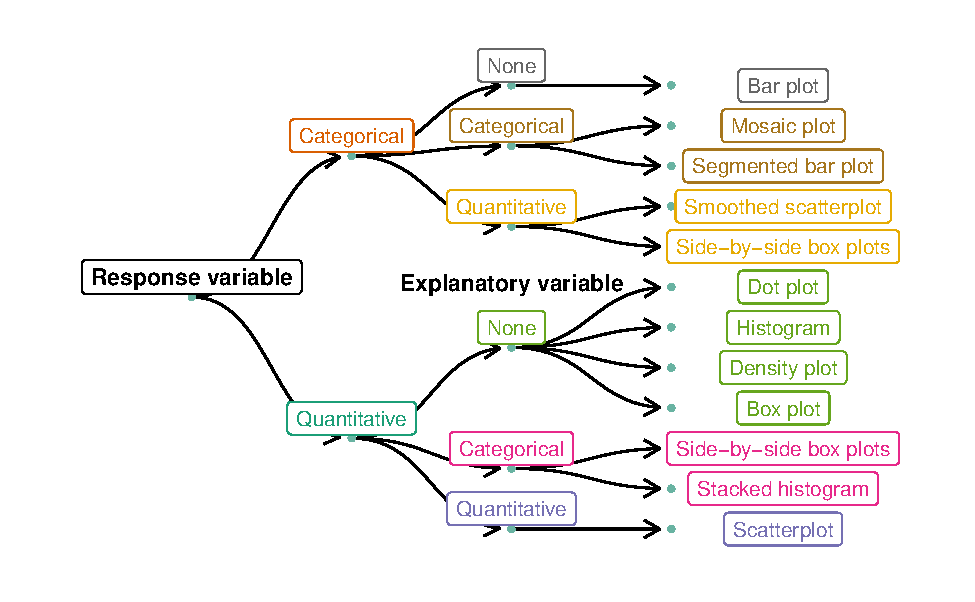
\includegraphics[width=0.7\linewidth]{04-RG-quantitative-data_files/figure-latex/decision-tree-plots-1} \end{center}

\newpage

\hypertarget{activity-4a-imdb-movie-reviews---displaying-one-variable}{%
\section{Activity 4a: IMDb Movie Reviews - Displaying One Variable}\label{activity-4a-imdb-movie-reviews---displaying-one-variable}}

\setstretch{1}

\hypertarget{learning-objectives}{%
\subsection{Learning objectives}\label{learning-objectives}}

\begin{itemize}
\item
  Identify and create appropriate summary statistics and plots
  given a data set or research question for quantitative data.
\item
  Interpret the following summary statistics in context:
  median, lower quartile, upper quartile,
  standard deviation, interquartile range.
\item
  Given a plot or set of plots, describe and compare the distribution(s)
  of a single quantitative variable
  (center, variability, shape, outliers).
\end{itemize}

\hypertarget{terminology-review-6}{%
\subsection{Terminology review}\label{terminology-review-6}}

In today's activity, we will review summary measures and plots for quantitative variables. Some terms covered in this activity are:

\begin{itemize}
\item
  Two measures of center: mean, median
\item
  Two measures of spread (variability): standard deviation, interquartile range (IQR)
\item
  Types of graphs: box plots, dot plots, histograms
\end{itemize}

To review these concepts, see Section 2.3 in the textbook.

\hypertarget{movies-released-in-2016}{%
\subsection{Movies released in 2016}\label{movies-released-in-2016}}

A data set was collected on movies released in 2016. Here is a list of some of the variables collected on these movies.

\begin{longtable}[]{@{}
  >{\raggedright\arraybackslash}p{(\columnwidth - 2\tabcolsep) * \real{0.24}}
  >{\raggedright\arraybackslash}p{(\columnwidth - 2\tabcolsep) * \real{0.76}}@{}}
\toprule
\textbf{Variable} & \textbf{Description} \\
\midrule
\endhead
\texttt{budget\_mil} & Amount of money (in US \$ millions) budgeted for the production of the movie \\
\texttt{revenue\_mil} & Amount of money (in US \$ millions) the movie made after release \\
\texttt{duration} & Length of the movie (in minutes) \\
\texttt{content\_rating} & Rating of the movie (\texttt{G}, \texttt{PG}, \texttt{PG-13}, \texttt{R}, \texttt{Not\ Rated}) \\
\texttt{imdb\_score} & IMDb user rating score from 1 to 10 \\
\texttt{genres} & Categories the movie falls into (e.g., Action, Drama, etc.) \\
\texttt{facebook\_likes} & Number of likes a movie receives on Facebook \\
\bottomrule
\end{longtable}

\newpage

\hypertarget{vocabulary-review.}{%
\subsubsection*{Vocabulary review.}\label{vocabulary-review.}}
\addcontentsline{toc}{subsubsection}{Vocabulary review.}

\begin{enumerate}
\def\labelenumi{\arabic{enumi}.}
\tightlist
\item
  What are the observational units in this data set?
\end{enumerate}

\vspace{0.1in}

\begin{enumerate}
\def\labelenumi{\arabic{enumi}.}
\setcounter{enumi}{1}
\tightlist
\item
  Which of the above listed variables are categorical?
\end{enumerate}

\vspace{.5in}

\begin{enumerate}
\def\labelenumi{\arabic{enumi}.}
\setcounter{enumi}{2}
\tightlist
\item
  Which of the above listed variables are quantitative?
\end{enumerate}

\vspace{.5in}

\hypertarget{summarizing-a-single-quantitative-variable}{%
\subsubsection*{Summarizing a single quantitative variable}\label{summarizing-a-single-quantitative-variable}}
\addcontentsline{toc}{subsubsection}{Summarizing a single quantitative variable}

The \texttt{favstats()} function from the \texttt{mosaic} package gives the summary statistics for a quantitative variable. Here we have the summary statistics for the variable \texttt{imdb\_score}. Highlight and run lines 1 -- 8 in the provided \texttt{R} script file to load the data set. Check that the summary statistics match that printed in the coursepack.

\begin{Shaded}
\begin{Highlighting}[]
\CommentTok{\# Read in data set}
\NormalTok{movies }\OtherTok{\textless{}{-}} \FunctionTok{read.csv}\NormalTok{(}\StringTok{"data/Movies2016.csv"}\NormalTok{) }
\NormalTok{movies }\SpecialCharTok{\%\textgreater{}\%} \CommentTok{\# Data set piped into...}
  \FunctionTok{summarise}\NormalTok{(}\FunctionTok{favstats}\NormalTok{(imdb\_score)) }\CommentTok{\# Apply favstats function to imdb\_score}
\end{Highlighting}
\end{Shaded}

\begin{verbatim}
#>   min   Q1 median  Q3 max     mean       sd  n missing
#> 1 3.4 5.65    6.4 7.1 8.2 6.309783 1.086689 92       0
\end{verbatim}

\begin{enumerate}
\def\labelenumi{\arabic{enumi}.}
\setcounter{enumi}{3}
\tightlist
\item
  Give the values for the two measures of center.
\end{enumerate}

\vspace{0.5in}

\begin{enumerate}
\def\labelenumi{\arabic{enumi}.}
\setcounter{enumi}{4}
\tightlist
\item
  Calculate the interquartile range (IQR = Q3 - Q1).
\end{enumerate}

\vspace{0.5in}

\begin{enumerate}
\def\labelenumi{\arabic{enumi}.}
\setcounter{enumi}{5}
\tightlist
\item
  Report the value of the standard deviation and interpret this value in context of the problem.
  \vspace{0.8in}
\end{enumerate}

\hypertarget{displaying-a-single-quantitative-variable}{%
\subsubsection*{Displaying a single quantitative variable}\label{displaying-a-single-quantitative-variable}}
\addcontentsline{toc}{subsubsection}{Displaying a single quantitative variable}

\begin{enumerate}
\def\labelenumi{\arabic{enumi}.}
\setcounter{enumi}{6}
\tightlist
\item
  What are the three types of plots used to plot a single quantitative variable?
\end{enumerate}

\newpage

A dotplot will plot a dot for each value in the data set. The following code will create a dotplot of IMDb scores. Notice that we put in the variable name \texttt{imdb\_score} for x = in the ggplot function.

\begin{Shaded}
\begin{Highlighting}[]
\NormalTok{movies }\SpecialCharTok{\%\textgreater{}\%} \CommentTok{\# Data set piped into...}
\FunctionTok{ggplot}\NormalTok{(}\FunctionTok{aes}\NormalTok{(}\AttributeTok{x =}\NormalTok{ imdb\_score)) }\SpecialCharTok{+}   \CommentTok{\# Name variable to plot}
  \FunctionTok{geom\_dotplot}\NormalTok{() }\SpecialCharTok{+}  \CommentTok{\# Create histogram with specified binwidth}
  \FunctionTok{labs}\NormalTok{(}\AttributeTok{title =} \StringTok{"Dotplot of IMDb Score of Movies in 2016"}\NormalTok{, }\CommentTok{\# Title for plot}
       \AttributeTok{x =} \StringTok{"IMDb Score"}\NormalTok{, }\CommentTok{\# Label for x axis}
       \AttributeTok{y =} \StringTok{"Frequency"}\NormalTok{) }\CommentTok{\# Label for y axis}
\end{Highlighting}
\end{Shaded}

\begin{center}\includegraphics[width=0.6\linewidth]{04-A05-EDA-1quantitative_files/figure-latex/unnamed-chunk-2-1} \end{center}

\begin{enumerate}
\def\labelenumi{\arabic{enumi}.}
\setcounter{enumi}{7}
\tightlist
\item
  What is the shape of the distribution of IMDb scores?
\end{enumerate}

\vspace{0.2in}

To create a histogram of the IMDb scores, enter the variable name, \texttt{imdb\_score} in the provided \texttt{R} script file for \texttt{variable} at line 20, highlight and run lines 19--24. Visually, this shows us the range of IMDb scores for Movies released in 2016.

Notice that the \textbf{bin width} is 0.5. For example the first bin consists of the number of movies in the data set with an IMDb score of 3.25 to 3.75. It is important to note that a movie with a IMDb score on the boundary of a bin will fall into the bin above it; for example, 4.76 would be counted in the bin 4.75--5.25.

\begin{Shaded}
\begin{Highlighting}[]
\NormalTok{movies }\SpecialCharTok{\%\textgreater{}\%} \CommentTok{\# Data set piped into...}
\FunctionTok{ggplot}\NormalTok{(}\FunctionTok{aes}\NormalTok{(}\AttributeTok{x =}\NormalTok{ variable)) }\SpecialCharTok{+}   \CommentTok{\# Name variable to plot}
  \FunctionTok{geom\_histogram}\NormalTok{(}\AttributeTok{binwidth =} \FloatTok{0.5}\NormalTok{) }\SpecialCharTok{+}  \CommentTok{\# Create histogram with specified binwidth}
  \FunctionTok{labs}\NormalTok{(}\AttributeTok{title =} \StringTok{"Histogram of IMDb Score of Movies in 2016"}\NormalTok{, }\CommentTok{\# Title for plot}
       \AttributeTok{x =} \StringTok{"IMDb Score"}\NormalTok{, }\CommentTok{\# Label for x axis}
       \AttributeTok{y =} \StringTok{"Frequency"}\NormalTok{) }\CommentTok{\# Label for y axis}
\end{Highlighting}
\end{Shaded}

\begin{enumerate}
\def\labelenumi{\arabic{enumi}.}
\setcounter{enumi}{8}
\tightlist
\item
  Sketch the histogram created here.
\end{enumerate}

\vspace{1.4in}

\begin{enumerate}
\def\labelenumi{\arabic{enumi}.}
\setcounter{enumi}{9}
\tightlist
\item
  Which range of IMDb scores have the highest frequency?
\end{enumerate}

\vspace{0.2in}

\begin{enumerate}
\def\labelenumi{\arabic{enumi}.}
\setcounter{enumi}{10}
\tightlist
\item
  Which five summary statistics are used in creating a box plot? \emph{Hint}: Together they are called the \textbf{five-number summary} of the variable.
\end{enumerate}

\vspace{0.4in}

\begin{enumerate}
\def\labelenumi{\arabic{enumi}.}
\setcounter{enumi}{11}
\item
  Using the code below we see that the three smallest IMDb scores in the data set are 3.4, 3.5, and 3.7 and the three largest IMDb scores are 8.0, 8.1, and 8.2:

\begin{Shaded}
\begin{Highlighting}[]
\NormalTok{movies }\SpecialCharTok{\%\textgreater{}\%} \CommentTok{\# Data set pipes into...}
  \FunctionTok{select}\NormalTok{(imdb\_score) }\SpecialCharTok{\%\textgreater{}\%} \CommentTok{\# Select imdb\_score variable}
  \FunctionTok{slice\_min}\NormalTok{(imdb\_score, }\AttributeTok{n =} \DecValTok{3}\NormalTok{)  }\CommentTok{\# Show 3 smallest values}
\end{Highlighting}
\end{Shaded}

\begin{verbatim}
#>   imdb_score
#> 1        3.4
#> 2        3.5
#> 3        3.7
\end{verbatim}

\begin{Shaded}
\begin{Highlighting}[]
\NormalTok{movies }\SpecialCharTok{\%\textgreater{}\%} \CommentTok{\# Data set pipes into...}
  \FunctionTok{select}\NormalTok{(imdb\_score) }\SpecialCharTok{\%\textgreater{}\%} \CommentTok{\# Select imdb\_score variable}
  \FunctionTok{slice\_max}\NormalTok{(imdb\_score, }\AttributeTok{n =} \DecValTok{3}\NormalTok{)  }\CommentTok{\# Show 3 largest values}
\end{Highlighting}
\end{Shaded}

\begin{verbatim}
#>   imdb_score
#> 1        8.2
#> 2        8.1
#> 3        8.0
\end{verbatim}

  Using the summary statistics above, and the smallest and largest values of the variable to check for outliers, sketch a box plot of IMDb Score. Be sure to label the axes.
\end{enumerate}

\vspace{1.5in}

\begin{enumerate}
\def\labelenumi{\arabic{enumi}.}
\setcounter{enumi}{12}
\item
  Compare the three graphs of IMDb scores created above.

  Which graph is best used to show the shape of the distribution?

  \vspace{0.5in}

  Which graph is best used to show the outliers of the distribution?

  \vspace{0.5in}
\end{enumerate}

\hypertarget{take-home-messages-5}{%
\subsection{Take-home messages}\label{take-home-messages-5}}

\begin{enumerate}
\def\labelenumi{\arabic{enumi}.}
\item
  Histograms, box plots, and dot plots can all be used to graphically display quantitative variables. When we have a single categorical variable and a single quantitative variable we will display the data in side-by-side plots.
\item
  The box plot is created using the five number summary: minimum value, quartile 1, median, quartile 3, and maximum value. Values in the data set that are less than \(Q_1 - 1.5*IQR\) and greater than \(Q_3 + 1.5*IQR\) are considering outliers and are graphically represented by a dot outside of the whiskers on the box plot.
\item
  Data should be summarized numerically and displayed graphically to give us information about the study.
\end{enumerate}

\hypertarget{additional-notes-4}{%
\subsection{Additional notes}\label{additional-notes-4}}

Use this space to summarize your thoughts and take additional notes on today's activity and material covered.

\newpage

\hypertarget{activity-4b-movie-budgets---displaying-two-variables}{%
\section{Activity 4b: Movie Budgets - Displaying Two Variables}\label{activity-4b-movie-budgets---displaying-two-variables}}

\setstretch{1}

\hypertarget{learning-objectives-1}{%
\subsection{Learning objectives}\label{learning-objectives-1}}

\begin{itemize}
\item
  Identify and create appropriate summary statistics and plots
  given a data set or research question for quantitative data.
\item
  Interpret the following summary statistics in context:
  median, lower quartile, upper quartile,
  standard deviation, interquartile range.
\item
  Given a plot or set of plots, describe and compare the distribution(s)
  of a single quantitative variable
  (center, variability, shape, outliers).
\end{itemize}

\hypertarget{terminology-review-7}{%
\subsection{Terminology review}\label{terminology-review-7}}

In today's activity, we will review summary measures and plots for a single categorical and single quantitative variable. Some terms covered in this activity are:

\begin{itemize}
\item
  Two measures of center: mean, median
\item
  Two measures of spread (variability): standard deviation, interquartile range (IQR)
\item
  Types of graphs: side-by-side: box plots, dot plots, histograms
\item
  Robust statistics
\end{itemize}

To review these concepts, see Section 2.3 in the textbook.

\hypertarget{movies-released-in-2016-1}{%
\subsection{Movies released in 2016}\label{movies-released-in-2016-1}}

We will again use the data set collected on movies released in 2016. As a reminder here is a list of some of the variables collected on these movies.

\begin{longtable}[]{@{}
  >{\raggedright\arraybackslash}p{(\columnwidth - 2\tabcolsep) * \real{0.24}}
  >{\raggedright\arraybackslash}p{(\columnwidth - 2\tabcolsep) * \real{0.76}}@{}}
\toprule
\textbf{Variable} & \textbf{Description} \\
\midrule
\endhead
\texttt{budget\_mil} & Amount of money (in US \$ millions) budgeted for the production of the movie \\
\texttt{revenue\_mil} & Amount of money (in US \$ millions) the movie made after release \\
\texttt{duration} & Length of the movie (in minutes) \\
\texttt{content\_rating} & Rating of the movie (\texttt{G}, \texttt{PG}, \texttt{PG-13}, \texttt{R}, \texttt{Not\ Rated}) \\
\texttt{imdb\_score} & IMDb user rating score from 1 to 10 \\
\texttt{genres} & Categories the movie falls into (e.g., Action, Drama, etc.) \\
\texttt{facebook\_likes} & Number of likes a movie receives on Facebook \\
\bottomrule
\end{longtable}

\newpage

To use the \texttt{favstats()} function in the mosaic package with two variables, we will enter the variables as a formula, response\textasciitilde explanatory. This function will give the summary statistics for budget for each content rating. Highlight and run lines 1 -- 9 in the provided \texttt{R} script file to load the data set and check that the summary statistics match those provided in the coursepack.

\begin{Shaded}
\begin{Highlighting}[]
\NormalTok{movies }\OtherTok{\textless{}{-}} \FunctionTok{read.csv}\NormalTok{(}\StringTok{"data/Movies2016.csv"}\NormalTok{)}
\NormalTok{movies }\SpecialCharTok{\%\textgreater{}\%} \CommentTok{\# Data set piped into...}
  \FunctionTok{filter}\NormalTok{(content\_rating }\SpecialCharTok{!=} \StringTok{"Not Rated"}\NormalTok{) }\SpecialCharTok{\%\textgreater{}\%} \CommentTok{\# Remove Not Rated movies}
  \FunctionTok{summarise}\NormalTok{(}\FunctionTok{favstats}\NormalTok{(budget\_mil}\SpecialCharTok{\textasciitilde{}}\NormalTok{content\_rating)) }\CommentTok{\# Apply favstats function to imdb\_score}
\end{Highlighting}
\end{Shaded}

\begin{verbatim}
#>   content_rating min    Q1 median      Q3 max     mean       sd  n missing
#> 1             PG 0.5 11.00   74.0 151.250 175 86.54167 71.52795 12       0
#> 2          PG-13 0.0 17.25   33.5 138.750 250 74.17500 74.15190 46       0
#> 3              R 0.0  7.75   19.5  29.625  60 21.09375 16.99926 32       0
\end{verbatim}

\begin{enumerate}
\def\labelenumi{\arabic{enumi}.}
\tightlist
\item
  Which content rating has the largest IQR?
\end{enumerate}

\vspace{0.8in}

\begin{enumerate}
\def\labelenumi{\arabic{enumi}.}
\setcounter{enumi}{1}
\tightlist
\item
  Report the mean budget amount for the PG rating.
\end{enumerate}

\vspace{0.3in}

\begin{enumerate}
\def\labelenumi{\arabic{enumi}.}
\setcounter{enumi}{2}
\tightlist
\item
  Report the mean budget amount for the R rating.
\end{enumerate}

\vspace{0.3in}

\begin{enumerate}
\def\labelenumi{\arabic{enumi}.}
\setcounter{enumi}{3}
\tightlist
\item
  Calculate the difference in mean budget amount for movies in 2016 with a PG rating minus those with a R rating. Use appropriate notation. Label group 1 as PG rating and group 2 as R rating.
\end{enumerate}

\vspace{0.8in}

\hypertarget{displaying-a-single-categorical-and-single-quantitative-variable}{%
\subsubsection*{Displaying a single categorical and single quantitative variable}\label{displaying-a-single-categorical-and-single-quantitative-variable}}
\addcontentsline{toc}{subsubsection}{Displaying a single categorical and single quantitative variable}

The boxplot of movie budgets (in millions) by content rating is plotted using the code below. Enter the variable \texttt{budget\_mil} for \texttt{response} and the variable \texttt{content\_rating} for explanatory at line 14, highlight and run code lines 12--18. This plot helps to compare the budget for different levels of content rating.

\begin{Shaded}
\begin{Highlighting}[]
\NormalTok{movies }\SpecialCharTok{\%\textgreater{}\%}  \CommentTok{\# Data set piped into...}
  \FunctionTok{filter}\NormalTok{(content\_rating }\SpecialCharTok{!=} \StringTok{"Not Rated"}\NormalTok{) }\SpecialCharTok{\%\textgreater{}\%} \CommentTok{\# Remove Not Rated movies}
  \FunctionTok{ggplot}\NormalTok{(}\FunctionTok{aes}\NormalTok{(}\AttributeTok{y =}\NormalTok{ response, }\AttributeTok{x =}\NormalTok{ explanatory))}\SpecialCharTok{+}  \CommentTok{\# Identify variables}
  \FunctionTok{geom\_boxplot}\NormalTok{()}\SpecialCharTok{+}  \CommentTok{\# Tell it to make a box plot}
  \FunctionTok{labs}\NormalTok{(}\AttributeTok{title =} \StringTok{"Side by side box plot of budget by content rating"}\NormalTok{,  }\CommentTok{\# Title}
       \AttributeTok{x =} \StringTok{"Content Rating"}\NormalTok{,    }\CommentTok{\# x{-}axis label}
       \AttributeTok{y =} \StringTok{"Budget (in Millions)"}\NormalTok{)  }\CommentTok{\# y{-}axis label}
\end{Highlighting}
\end{Shaded}

\begin{enumerate}
\def\labelenumi{\arabic{enumi}.}
\setcounter{enumi}{4}
\tightlist
\item
  Sketch the box plots created using the \texttt{R} code.
\end{enumerate}

\vspace{1.5in}

\begin{enumerate}
\def\labelenumi{\arabic{enumi}.}
\setcounter{enumi}{5}
\item
  Answer the following questions about the box plots created.

  \begin{enumerate}
  \def\labelenumii{\alph{enumii}.}
  \item
    Which content rating has the highest center?
    \vspace{0.2in}
  \item
    Which content rating has the largest spread?
    \vspace{0.2in}
  \item
    Which content rating has the most skewed distribution?
    \vspace{0.2in}
  \item
    Fifty percent of movies in 2016 with a PG-13 content rating fall below what value? What is the name of this value?
    \vspace{0.4in}
  \item
    What is the value for the third quartile (Q3) for the PG-13 rating? Interpret this value in context.
    \vspace{.8in}
  \end{enumerate}
\item
  Which variable is the explanatory variable? Response variable?
\end{enumerate}

\vspace{0.4in}

\hypertarget{robust-statistics}{%
\subsubsection{Robust Statistics}\label{robust-statistics}}

Let's examine how the presence of outliers affect the values of center and spread. For this part of the activity we will look at the variable \texttt{revenue} in the movies data set.

\begin{verbatim}
#>   min       Q1   median       Q3      max     mean       sd  n missing
#> 1   0 1.467318 33.02703 73.13457 407.1973 61.87334 89.57824 92       0
\end{verbatim}

\begin{Shaded}
\begin{Highlighting}[]
\NormalTok{movies }\SpecialCharTok{\%\textgreater{}\%} \CommentTok{\# Data set piped into...}
\FunctionTok{ggplot}\NormalTok{(}\FunctionTok{aes}\NormalTok{(}\AttributeTok{x =}\NormalTok{ revenue\_mil)) }\SpecialCharTok{+}   \CommentTok{\# Name variable to plot}
  \FunctionTok{geom\_boxplot}\NormalTok{() }\SpecialCharTok{+}  \CommentTok{\# Create histogram with specified binwidth}
  \FunctionTok{labs}\NormalTok{(}\AttributeTok{title =} \StringTok{"Histogram of Revenue of Movies in 2016"}\NormalTok{, }\CommentTok{\# Title for plot}
       \AttributeTok{x =} \StringTok{"Revenue (in Millions)"}\NormalTok{, }\CommentTok{\# Label for x axis}
       \AttributeTok{y =} \StringTok{"Frequency"}\NormalTok{) }\CommentTok{\# Label for y axis}
\end{Highlighting}
\end{Shaded}

\begin{center}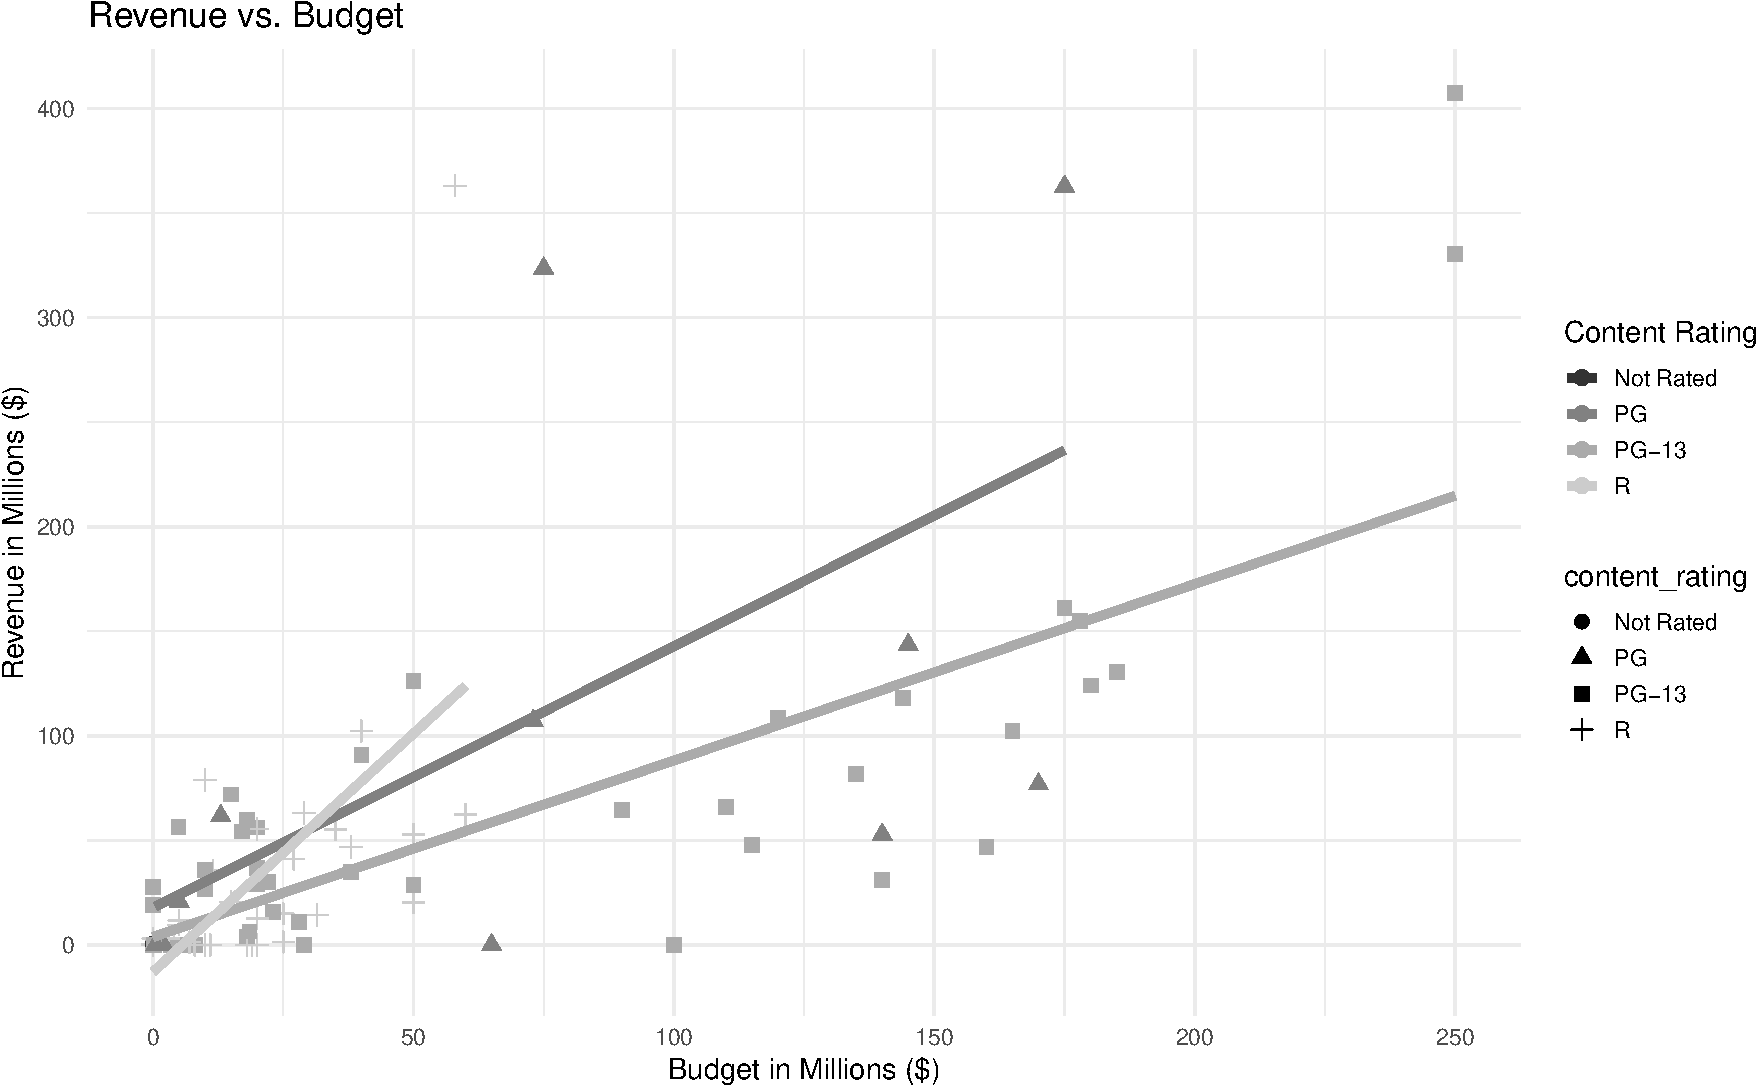
\includegraphics[width=0.6\linewidth]{04-A06-EDA-1cat_1quant_files/figure-latex/unnamed-chunk-4-1} \end{center}

\begin{enumerate}
\def\labelenumi{\arabic{enumi}.}
\setcounter{enumi}{7}
\tightlist
\item
  Report the two measures of center for this data.
\end{enumerate}

\vspace{0.8in}

\begin{enumerate}
\def\labelenumi{\arabic{enumi}.}
\setcounter{enumi}{8}
\tightlist
\item
  Report the two measures of spread for this data.
\end{enumerate}

\vspace{0.8in}

To show the effect of outliers on the measures of center and spread, the largest values in the data set were reduced by 100 \$MM. Upload and import the data set, \texttt{Movies2016\_Sub} into Rstudio. Enter the variable name \texttt{revenue\_mil} for \texttt{variable} in line 32 and 34 to summarize and create a boxplot of the data. Highlight and run lines 31--38.

\begin{Shaded}
\begin{Highlighting}[]
\NormalTok{Movies2016\_Sub }\SpecialCharTok{\%\textgreater{}\%} \CommentTok{\# Data set piped into...}
  \FunctionTok{summarise}\NormalTok{(}\FunctionTok{favstats}\NormalTok{(variable))}
\end{Highlighting}
\end{Shaded}

\begin{Shaded}
\begin{Highlighting}[]
\NormalTok{Movies2016\_Sub }\SpecialCharTok{\%\textgreater{}\%} \CommentTok{\# Data set piped into...}
\FunctionTok{ggplot}\NormalTok{(}\FunctionTok{aes}\NormalTok{(}\AttributeTok{x =}\NormalTok{ variable)) }\SpecialCharTok{+}   \CommentTok{\# Name variable to plot}
  \FunctionTok{geom\_boxplot}\NormalTok{() }\SpecialCharTok{+}  \CommentTok{\# Create histogram with specified binwidth}
  \FunctionTok{labs}\NormalTok{(}\AttributeTok{title =} \StringTok{"Histogram of Revenue of Movies in 2016"}\NormalTok{, }\CommentTok{\# Title for plot}
       \AttributeTok{x =} \StringTok{"Revenue (in Millions)"}\NormalTok{, }\CommentTok{\# Label for x axis}
       \AttributeTok{y =} \StringTok{"Frequency"}\NormalTok{) }\CommentTok{\# Label for y axis}
\end{Highlighting}
\end{Shaded}

\begin{enumerate}
\def\labelenumi{\arabic{enumi}.}
\setcounter{enumi}{9}
\tightlist
\item
  Report the two measures of center for this new data set.
\end{enumerate}

\vspace{0.8in}

\begin{enumerate}
\def\labelenumi{\arabic{enumi}.}
\setcounter{enumi}{10}
\tightlist
\item
  Report the two measures of spread for this new data set.
\end{enumerate}

\vspace{0.8in}

\begin{enumerate}
\def\labelenumi{\arabic{enumi}.}
\setcounter{enumi}{11}
\tightlist
\item
  Which measure of center is robust to outliers? Explain your answer.
\end{enumerate}

\vspace{0.5in}

\begin{enumerate}
\def\labelenumi{\arabic{enumi}.}
\setcounter{enumi}{12}
\tightlist
\item
  Which measure of spread is robust to outliers? Explain your answer.
\end{enumerate}

\vspace{0.5in}

\hypertarget{take-home-messages-6}{%
\subsection{Take-home messages}\label{take-home-messages-6}}

\begin{enumerate}
\def\labelenumi{\arabic{enumi}.}
\item
  When comparing distributions of quantitative variables we look at the shape, center, spread, and for outliers. There are two measures of center: mean and the median and two measures of spread: standard deviation and the interquartile range, IQR = Q1- Q3.
\item
  The median and the interquartile range are robust statistics, meaning that they are not affected by very large or very small values. When we have a skewed distribution the best measure of center is the median and the best measure of spread is the IQR.
\end{enumerate}

\hypertarget{additional-notes-5}{%
\subsection{Additional notes}\label{additional-notes-5}}

Use this space to summarize your thoughts and take additional notes on today's activity and material covered.

\newpage

\hypertarget{week-4-lab-ipeds}{%
\section{Week 4 Lab: IPEDs}\label{week-4-lab-ipeds}}

\setstretch{1}

\hypertarget{learning-objectives-2}{%
\subsection{Learning objectives}\label{learning-objectives-2}}

\begin{itemize}
\item
  Identify and create appropriate summary statistics and plots
  given a data set or research question for quantitative data.
\item
  Interpret the following summary statistics in context:
  median, lower quartile, upper quartile,
  standard deviation, interquartile range.
\item
  Given a plot or set of plots, describe and compare the distribution(s)
  of a single quantitative variable
  (center, variability, shape, outliers).
\item
  Get practice using \texttt{R} to create graphs of quantitative variables.
\end{itemize}

\hypertarget{ipeds}{%
\subsection{IPEDS}\label{ipeds}}

Download and open the provided \texttt{R} script file for week 4 lab to answer the following questions. \textbf{Remember that bolded questions will be answered on Gradescope for your group.}

These data are on a subset of institutions that met the following selection criteria:

\begin{itemize}
\item
  Degree granting
\item
  United States only
\item
  Title IV participating
\item
  Not for profit
\item
  2-year or 4-year or above
\item
  Has full-time first-time undergraduates
\item
  Note that several variables have missing values for some institutions (denoted by ``NA'').
\end{itemize}

\begin{center}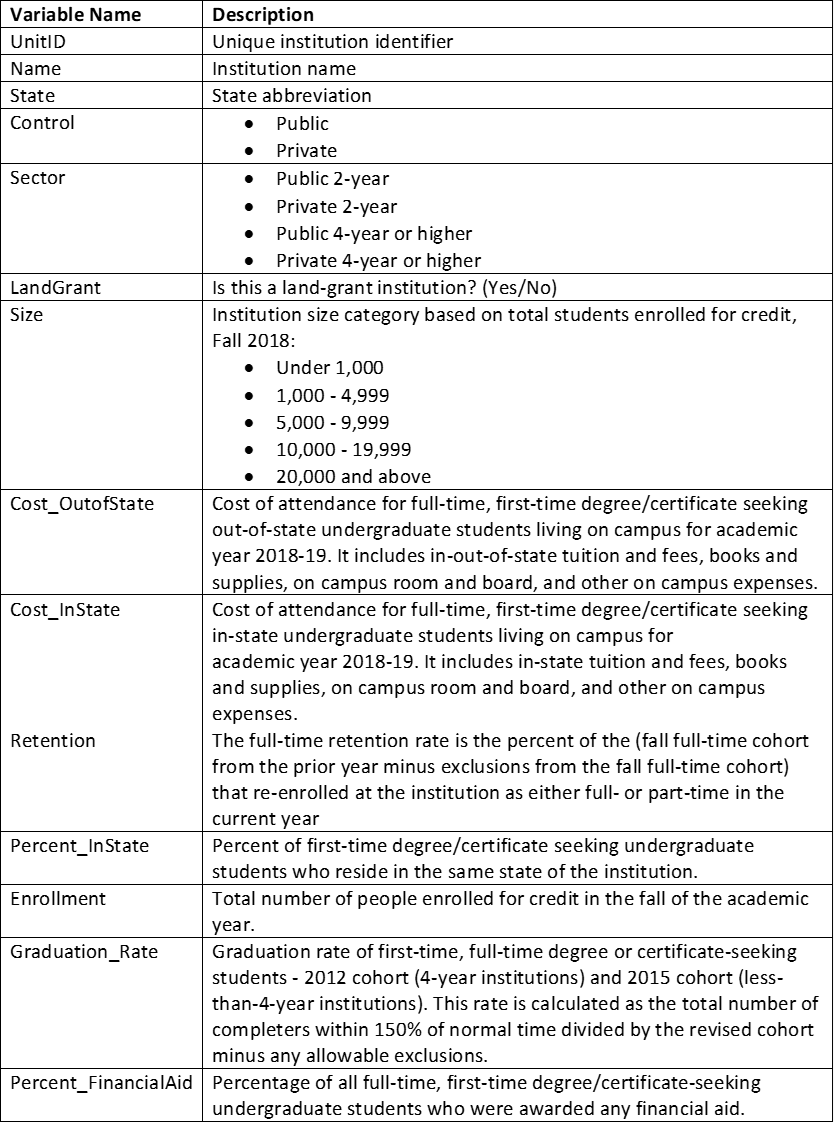
\includegraphics[width=0.75\linewidth]{images/IPEDS_Description} \end{center}

\begin{enumerate}
\def\labelenumi{\arabic{enumi}.}
\tightlist
\item
  What are the observational units for this study?
\end{enumerate}

\vspace{0.3in}

\begin{enumerate}
\def\labelenumi{\arabic{enumi}.}
\setcounter{enumi}{1}
\tightlist
\item
  Using the above table, which variables are categorical?
\end{enumerate}

\vspace{1in}

\begin{enumerate}
\def\labelenumi{\arabic{enumi}.}
\setcounter{enumi}{2}
\tightlist
\item
  Which variables are quantitative?
\end{enumerate}

\vspace{1in}

\begin{enumerate}
\def\labelenumi{\arabic{enumi}.}
\setcounter{enumi}{3}
\tightlist
\item
  What type of graph(s) could be used to plot retention rate?
\end{enumerate}

\vspace{0.5in}

Upload and import the data set \texttt{IPEDS\_Data\_2018}. Enter the name of the data set (see the environment tab) for \texttt{datasetname} in the \texttt{R} script file in line 5. We will look at the retention rates for the different institutions. Enter the variable name \texttt{Retention} for \texttt{variable} in line 12. Highlight and run lines 1 -- 12.

\begin{Shaded}
\begin{Highlighting}[]
\NormalTok{datasetname }\OtherTok{{-}\textgreater{}}\NormalTok{ IPEDS }\CommentTok{\#Creates the object IPEDS }
\NormalTok{IPEDS }\OtherTok{\textless{}{-}}\NormalTok{ IPEDS }\SpecialCharTok{\%\textgreater{}\%}
  \FunctionTok{filter}\NormalTok{(Sector }\SpecialCharTok{!=} \StringTok{"Public 2{-}year"}\NormalTok{) }\CommentTok{\#Filters the data set to remove Public 2{-}year}
\NormalTok{IPEDS }\OtherTok{\textless{}{-}}\NormalTok{ IPEDS }\SpecialCharTok{\%\textgreater{}\%}
  \FunctionTok{filter}\NormalTok{(Sector }\SpecialCharTok{!=} \StringTok{"Private 2{-}year"}\NormalTok{) }\CommentTok{\#Filters the data set to remove Private 2{-}year}
\NormalTok{IPEDS }\SpecialCharTok{\%\textgreater{}\%}
  \FunctionTok{summarise}\NormalTok{(}\FunctionTok{favstats}\NormalTok{(variable)) }\CommentTok{\#Gives the summary statistics}
\end{Highlighting}
\end{Shaded}

\textbf{5. Report the value for quartile 3 and interpret this value in context of the study.}

\vspace{1in}

\begin{enumerate}
\def\labelenumi{\arabic{enumi}.}
\setcounter{enumi}{5}
\tightlist
\item
  Calculate the interquartile range for this study.
\end{enumerate}

\vspace{0.5in}

\begin{enumerate}
\def\labelenumi{\arabic{enumi}.}
\setcounter{enumi}{6}
\tightlist
\item
  Report and interpret the value of the standard deviation.
\end{enumerate}

\vspace{1in}

\begin{enumerate}
\def\labelenumi{\arabic{enumi}.}
\setcounter{enumi}{7}
\tightlist
\item
  How many missing values are there? What does this indicate?
\end{enumerate}

\vspace{0.8in}

Next we will create both a histogram and a boxplot of the variable \texttt{Retention}. Enter the name of the variable in both line 16 and line 23 for \texttt{variable} in the \texttt{R} script file. \textbf{Give each plot a descriptive title.} Highlight and run lines 15 -- 27 to give the histogram and boxplot. \textbf{Export and upload both plots to Gradescope for your group.}

\begin{Shaded}
\begin{Highlighting}[]
\NormalTok{IPEDS }\SpecialCharTok{\%\textgreater{}\%} \CommentTok{\# Data set piped into...}
\FunctionTok{ggplot}\NormalTok{(}\FunctionTok{aes}\NormalTok{(}\AttributeTok{x =}\NormalTok{ variable)) }\SpecialCharTok{+}   \CommentTok{\# Name variable to plot}
  \FunctionTok{geom\_histogram}\NormalTok{(}\AttributeTok{binwidth =} \DecValTok{5}\NormalTok{) }\SpecialCharTok{+}  \CommentTok{\# Create dotplot}
  \FunctionTok{labs}\NormalTok{(}\AttributeTok{title =} \StringTok{"Title"}\NormalTok{, }\CommentTok{\# Title for plot}
       \AttributeTok{x =} \StringTok{"Rentention Rate"}\NormalTok{, }\CommentTok{\# Label for x axis}
       \AttributeTok{y =} \StringTok{"Frequency"}\NormalTok{) }\CommentTok{\# Label for y axis}
\end{Highlighting}
\end{Shaded}

\begin{Shaded}
\begin{Highlighting}[]
\NormalTok{IPEDS }\SpecialCharTok{\%\textgreater{}\%} \CommentTok{\# Data set piped into...}
\FunctionTok{ggplot}\NormalTok{(}\FunctionTok{aes}\NormalTok{(}\AttributeTok{x =}\NormalTok{ variable)) }\SpecialCharTok{+}   \CommentTok{\# Name variable to plot}
  \FunctionTok{geom\_boxplot}\NormalTok{() }\SpecialCharTok{+}  \CommentTok{\# Create dotplot}
  \FunctionTok{labs}\NormalTok{(}\AttributeTok{title =} \StringTok{"Title"}\NormalTok{, }\CommentTok{\# Title for plot}
       \AttributeTok{x =} \StringTok{"Retention Rates"}\NormalTok{, }\CommentTok{\# Label for x axis}
       \AttributeTok{y =} \StringTok{"Frequency"}\NormalTok{) }\CommentTok{\# Label for y axis}
\end{Highlighting}
\end{Shaded}

\begin{enumerate}
\def\labelenumi{\arabic{enumi}.}
\setcounter{enumi}{8}
\tightlist
\item
  What is the shape of the distribution of retention rates?
\end{enumerate}

\vspace{0.3in}

\begin{enumerate}
\def\labelenumi{\arabic{enumi}.}
\setcounter{enumi}{9}
\tightlist
\item
  Identify any outliers in the data set.
\end{enumerate}

\vspace{0.3in}

In the next part of the activity we will compare retention rates for public and private institutions. Note that this variable is \texttt{Control} in the data set.

\textbf{11. Which variable will we treat as the explanatory variable? Response variable?}

\vspace{0.8in}

Enter the name of the explanatory variable and the name of the response variable in lines 31 and 34 of the \texttt{R} script file. Highlight and run lines 30 -- 38 to find the summary statistics and create side by side boxplots of the data.

\begin{Shaded}
\begin{Highlighting}[]
\NormalTok{IPEDS }\SpecialCharTok{\%\textgreater{}\%}  \CommentTok{\# Data set piped into...}
  \FunctionTok{summarise}\NormalTok{(}\FunctionTok{favstats}\NormalTok{(response}\SpecialCharTok{\textasciitilde{}}\NormalTok{explanatory)) }\CommentTok{\# Apply favstats function to budget\_mil and content rating}
\end{Highlighting}
\end{Shaded}

\begin{Shaded}
\begin{Highlighting}[]
\NormalTok{IPEDS }\SpecialCharTok{\%\textgreater{}\%}  \CommentTok{\# Data set piped into...}
  \FunctionTok{ggplot}\NormalTok{(}\FunctionTok{aes}\NormalTok{(}\AttributeTok{y =}\NormalTok{ response, }\AttributeTok{x =}\NormalTok{ explanatory))}\SpecialCharTok{+}  \CommentTok{\# Identify variables}
  \FunctionTok{geom\_boxplot}\NormalTok{()}\SpecialCharTok{+}  \CommentTok{\# Tell it to make a box plot}
  \FunctionTok{labs}\NormalTok{(}\AttributeTok{title =} \StringTok{"Side by side box plot of retention rates control"}\NormalTok{,  }\CommentTok{\# Title}
       \AttributeTok{x =} \StringTok{"Control"}\NormalTok{,    }\CommentTok{\# x{-}axis label}
       \AttributeTok{y =} \StringTok{"Retention Rates"}\NormalTok{)  }\CommentTok{\# y{-}axis label}
\end{Highlighting}
\end{Shaded}

\begin{enumerate}
\def\labelenumi{\arabic{enumi}.}
\setcounter{enumi}{11}
\item
  Compare the two boxplots.

  Which type of university has the highest center?
  \vspace{0.3in}

  Largest spread?
  \vspace{0.3in}

  What is the shape of each distribution?
  \vspace{0.3in}

  Does either distribution have outliers?
  \vspace{0.3in}
\end{enumerate}

\textbf{13. Report the difference in mean retention rates for private and public universities. Use private minus public as the order of subtraction. Use the appropriate notation.}

\vspace{0.8in}

\begin{enumerate}
\def\labelenumi{\arabic{enumi}.}
\setcounter{enumi}{13}
\tightlist
\item
  Does there appear to be an association between retention rates and type of university? Explain.
\end{enumerate}

\vspace{0.8in}

The following set of code will create side by side boxplots of retention rates by size of the university. Highlight and run lines 41--46 in the \texttt{R} script file.

\begin{Shaded}
\begin{Highlighting}[]
\NormalTok{IPEDS }\SpecialCharTok{\%\textgreater{}\%}  \CommentTok{\# Data set piped into...}
  \FunctionTok{ggplot}\NormalTok{(}\FunctionTok{aes}\NormalTok{(}\AttributeTok{y =}\NormalTok{ Retention, }\AttributeTok{x =}\NormalTok{ Size))}\SpecialCharTok{+}  \CommentTok{\# Identify variables}
  \FunctionTok{geom\_boxplot}\NormalTok{()}\SpecialCharTok{+}  \CommentTok{\# Tell it to make a box plot}
  \FunctionTok{labs}\NormalTok{(}\AttributeTok{title =} \StringTok{"Side by side box plot of retention rates by size"}\NormalTok{,  }\CommentTok{\# Title}
       \AttributeTok{x =} \StringTok{"Size"}\NormalTok{,    }\CommentTok{\# x{-}axis label}
       \AttributeTok{y =} \StringTok{"Retention Rates"}\NormalTok{)  }\CommentTok{\# y{-}axis label}
\end{Highlighting}
\end{Shaded}

\begin{enumerate}
\def\labelenumi{\arabic{enumi}.}
\setcounter{enumi}{14}
\tightlist
\item
  Is size a categorical or quantitative variable?
\end{enumerate}

\vspace{0.5in}

\begin{enumerate}
\def\labelenumi{\arabic{enumi}.}
\setcounter{enumi}{15}
\tightlist
\item
  Which university size has the highest center for retention rates?
\end{enumerate}

\vspace{0.5in}

\begin{enumerate}
\def\labelenumi{\arabic{enumi}.}
\setcounter{enumi}{16}
\tightlist
\item
  Which university size has the largest spread of retention rates?
\end{enumerate}

\vspace{0.5in}

\newpage

\hypertarget{exploring-multivariable-data}{%
\chapter{Exploring Multivariable Data}\label{exploring-multivariable-data}}

\hypertarget{week-5---reading-guide-quantitative-data}{%
\section{Week 5 - Reading Guide: Quantitative Data}\label{week-5---reading-guide-quantitative-data}}

\hypertarget{section-3.1-fitting-a-line-residuals-and-correlation}{%
\subsection*{Section 3.1 (Fitting a line, residuals, and correlation)}\label{section-3.1-fitting-a-line-residuals-and-correlation}}
\addcontentsline{toc}{subsection}{Section 3.1 (Fitting a line, residuals, and correlation)}

\setstretch{1}

\textbf{Videos}

\begin{itemize}
\tightlist
\item
  Chapter3
\end{itemize}

\setstretch{1.25}

\hypertarget{reminders-from-section-2.3}{%
\subsubsection*{Reminders from Section 2.3}\label{reminders-from-section-2.3}}
\addcontentsline{toc}{subsubsection}{Reminders from Section 2.3}

Scatterplot: displays two quantitative variables; one dot = two measurements (\(x\), \(y\)) on one observational unit.

Four characteristics of a scatterplot:
\setstretch{1}

\begin{itemize}
\tightlist
\item
  \emph{Form}: pattern of the dots plotted. Is the trend generally linear (you can fit a straight line to the data) or non-linear?\\
\item
  \emph{Strength}: how closely do the points follow a trend? Very closely (strong)? No pattern (weak)?\\
\item
  \emph{Direction}: as the \(x\) values increase, do the \(y\)-values tend to increase (positive) or decrease (negative)?\\
\item
  Unusual observations or \emph{outliers}: points that do not fit the overall pattern of the data.
\end{itemize}

\setstretch{1.25}

\hypertarget{vocabulary-6}{%
\subsubsection*{Vocabulary}\label{vocabulary-6}}
\addcontentsline{toc}{subsubsection}{Vocabulary}

Residual:
\rgs

\rgi Formula:
\rgs

Residual plot:
\rgs

Correlation:
\rgs

\hypertarget{notes-8}{%
\subsubsection*{Notes}\label{notes-8}}
\addcontentsline{toc}{subsubsection}{Notes}

General equation of a linear regression for a \emph{population}: \(y= \beta_0+ \beta_1 x+\epsilon\), where

\rgi \(x\) represents
\rgs

\rgi \(y\) represents
\rgs

\rgi \(\beta_0\) represents
\rgs

\rgi \(\beta_1\) represents
\rgs

\rgi \(\epsilon\) represents
\rgs

General equation of a linear regression model from \emph{sample} data: \(\hat{y}= b_0+ b_1 x\), where

\rgi \(x\) represents
\rgs

\rgi \(\hat{y}\) represents
\rgs

\rgi \(b_0\) represents
\rgs

\rgi \(b_1\) represents
\rgs

Fill in the following table with the appropriate notation for each summary measure.

\begin{center}
\begin{tabular}{|l|p{2in}|p{2in}|} \hline
Summary Measure & Parameter & Statistic \\ \hline
Correlation & & \\ 
& & \\ \hline
Slope & & \\ 
& & \\ \hline
$y$-intercept & & \\ 
& & \\ \hline
\end{tabular}
\end{center}

Fill in the blanks below to define some of the properties of correlation:

\rgi The value of correlation must be between \_\_\_\_\_\_\_\_\_\_\_. (Includes the endpoints of the interval)

\rgi The sign of correlation gives the \_\_\_\_\_\_\_\_\_\_\_\_\_\_ of the linear relationship.

\rgi The magnitude of correlation gives the \_\_\_\_\_\_\_\_\_\_\_\_ of the linear relationship.

True or false: A scatterplot that shows random scatter would be considered non-linear.

True or false: If the correlation between two quantitative variables is equal to zero, then the two variables are not associated.

True or false: To calculate a predicted \(y\)-value from a given \(x\)-value, just look at the scatterplot and estimate the \(y\)-value.

True or false: A positive residual indicates the data point is above the regression line.

\newpage

\hypertarget{example-brushtail-possums}{%
\subsubsection*{Example: Brushtail possums}\label{example-brushtail-possums}}
\addcontentsline{toc}{subsubsection}{Example: Brushtail possums}

\begin{enumerate}
\def\labelenumi{\arabic{enumi}.}
\item
  What are the observational units?\\
  \rgs
\item
  Look at the scatterplot in Figure 3.5.
\end{enumerate}

\rgi a) What is the explanatory variable? The response variable? What type is each?
\rgs

\rgi b) What is the form of the scatterplot?
\rgs

\rgi c) What is the direction of the scatterplot?
\rgs

\rgi d) What is the strength of the scatterplot?
\rgs

\rgi e) Are there any outliers on the scatterplot?
\rgs

\begin{enumerate}
\def\labelenumi{\arabic{enumi}.}
\setcounter{enumi}{2}
\item
  Write the equation of the regression line, in context (do not use \(x\) and \(y\), use variable names instead).
  \rgs
\item
  Calculate the predicted head length for a possum with a 76.0 cm total length.
  \rgs
\item
  One of the possums in the data set has a total length of 76.0 cm and a head length of 85.1 cm. Calculate the residual for this possum. Does this possum lie above or below the regression line?
  \rgs
\end{enumerate}

\hypertarget{section-3.2-least-squares-regression}{%
\subsection*{Section 3.2 (Least squares regression)}\label{section-3.2-least-squares-regression}}
\addcontentsline{toc}{subsection}{Section 3.2 (Least squares regression)}

\setstretch{1}

You may skip the special topic Sections 3.2.3.1 and 3.2.6.

\textbf{Videos}

\begin{itemize}
\tightlist
\item
  Chapter3
\end{itemize}

\setstretch{1.25}

\hypertarget{vocabulary-7}{%
\subsubsection*{Vocabulary}\label{vocabulary-7}}
\addcontentsline{toc}{subsubsection}{Vocabulary}

Least squares criterion:
\rgs

Least squares line:
\rgs

\texttt{lm()} \texttt{R} function:
\rgi \texttt{name\_of\_model\ \textless{}-\ lm(response\ \textasciitilde{}\ explanatory,\ data\ =\ data\_set\_name)}

\rgs

slope:
\rgs

\(y\)-intercept:\\
\rgs

Extrapolation:

\rgi Assumes the pattern seen in the data extends beyond the data collected!

Coefficient of determination:

\rgi \(s_y^2\) (or SST) represents
\rgs

\rgi \(s_{RES}^2\) (or SSE) represents
\rgs

\hypertarget{notes-9}{%
\subsubsection*{Notes}\label{notes-9}}
\addcontentsline{toc}{subsubsection}{Notes}

Two methods for determining the best line:

\rgi 1.
\rgs

\rgi 2.
\rgs

Notation for the coefficient of determination:
\rgs

Formulas for calculating the coefficient of determination:
\rgs

True or false: A correlation between two quantitative variables implies a causal relationship exists between the variables.

True or false: The slope of the line tells us how much to expect the \(y\) variable to increase or decrease when the \(x\) variable increases by 1 unit.

True or false: The coefficient of determination is just the square of the correlation.

\hypertarget{example-elmhurst-college}{%
\subsubsection*{Example: Elmhurst College}\label{example-elmhurst-college}}
\addcontentsline{toc}{subsubsection}{Example: Elmhurst College}

\begin{enumerate}
\def\labelenumi{\arabic{enumi}.}
\item
  What are the observational units?\\
  \rgs
\item
  Look at the scatterplot in Figure 3.13.
\end{enumerate}

\rgi a) What is the explanatory variable? The response variable?\\
\rgs

\rgi b) What is the form of the scatterplot?\\
\rgs

\rgi c) What is the direction of the scatterplot?
\rgs

\rgi d) What is the strength of the scatterplot?
\rgs

\rgi e) Are there any outliers on the scatterplot?\\
\rgs

\begin{enumerate}
\def\labelenumi{\arabic{enumi}.}
\setcounter{enumi}{2}
\item
  Write the equation of the regression line, in context (do not use \(x\) and \(y\), use variable names instead).
  \rgs
\item
  Interpret the slope of the line, in the context of the problem. Remember that both family income and gift aid from the university are measured in \$1000s.
  \rgs
  \rgs
\item
  Interpret the \(y\)-intercept of the line, in the context of the problem. Remember that both family income and gift aid from the university are measured in \$1000s.
  \rgs
  \rgs
\item
  Is your interpretation in question 5 an example of extrapolation?
  \rgs
\item
  Give and interpret, in context, the value of the coefficient of determination.
  \rgs
  \rgs
\end{enumerate}

\hypertarget{section-3.3-outliers-in-linear-regression}{%
\subsection*{Section 3.3 (Outliers in linear regression)}\label{section-3.3-outliers-in-linear-regression}}
\addcontentsline{toc}{subsection}{Section 3.3 (Outliers in linear regression)}

\setstretch{1}

\textbf{Videos}

\begin{itemize}
\tightlist
\item
  Chapter3
\end{itemize}

\setstretch{1.25}

\hypertarget{vocabulary-8}{%
\subsubsection*{Vocabulary}\label{vocabulary-8}}
\addcontentsline{toc}{subsubsection}{Vocabulary}

Outlier:
\rgs

Leverage:
\rgs

Influential:
\rgs

\hypertarget{notes-10}{%
\subsubsection*{Notes}\label{notes-10}}
\addcontentsline{toc}{subsubsection}{Notes}

Investigate, but do not remove, outliers. Unless you find there was an actual error in the data collection, ignoring outliers can make models poor predictors!

True or false: All high leverage outliers are influential.

True or false: An outlier is considered high leverage if it is extreme in its \(x\)-value.

\hypertarget{section-3.4-r-correlation-and-regression-and-section-3.5-chapter-3-review}{%
\subsection*{Section 3.4 (R: Correlation and regression) and Section 3.5 (Chapter 3 review)}\label{section-3.4-r-correlation-and-regression-and-section-3.5-chapter-3-review}}
\addcontentsline{toc}{subsection}{Section 3.4 (R: Correlation and regression) and Section 3.5 (Chapter 3 review)}

\setstretch{1}

\textbf{Videos}

\begin{itemize}
\tightlist
\item
  Chapter3
\end{itemize}

\setstretch{1.25}

Section 3.4 presents five tutorials on analyzing two quantitative variables in \texttt{R}. We recommend you complete all five.

\hypertarget{notes-11}{%
\subsubsection*{Notes}\label{notes-11}}
\addcontentsline{toc}{subsubsection}{Notes}

Statistics summarize
\rgs

Parameters summarize
\rgs

What are the two ways to calculate the coefficient of determination?
\rgs

What is the formula for calculating a residual?
\rgs

Determine whether each of the following statements about the correlation coefficient are true or false:

\begin{enumerate}
\def\labelenumi{\arabic{enumi}.}
\item
  The correlation coefficient must be a positive number.
\item
  Stronger linear relationships are indicated by correlation coefficients far from 0.
\item
  The correlation coefficient is a robust statistic.
\item
  When two variables are highly correlated, that indicates a causal relationship exists between the variables.
\item
  The sign of the correlation coefficient will be the same as the sign of the regression line slope, though the values are typically different.
\end{enumerate}

Fill in the blanks to correctly interpret:

\begin{itemize}
\item
  Slope:

  For every \_\_\_\_\_\_\_\_\_\_\_\_\_\_\_\_\_\_\_\_\_\_\_\_\_\_\_\_, we expect \_\_\_\_\_\_\_\_\_\_\_\_\_\_\_\_\_ to increase (if slope is \_\_\_\_\_\_\_\_\_\_\_\_\_) or decrease (if slope is \_\_\_\_\_\_\_\_\_\_\_\_) by the absolute value of the \_\_\_\_\_\_\_\_\_.
\item
  \(y\)-intercept:

  If \_\_\_\_\_\_\_\_\_\_\_\_\_\_\_, we predict the \_\_\_\_\_\_\_\_\_\_\_\_\_\_\_\_\_\_\_\_\_\_\_\_\_\_ to equal \_\_\_\_\_\_\_\_\_\_.
\end{itemize}

Look at the table of vocabulary terms. If there are any you do not know, be sure to review the appropriate section of your text.

\hypertarget{section-4.1-gapminder-world}{%
\subsection*{Section 4.1 (Gapminder world)}\label{section-4.1-gapminder-world}}
\addcontentsline{toc}{subsection}{Section 4.1 (Gapminder world)}

\setstretch{1}

\textbf{Videos}

\begin{itemize}
\tightlist
\item
  Chapter4
\end{itemize}

\setstretch{1.25}

\hypertarget{reminder-from-section-3.1}{%
\subsubsection*{Reminder from Section 3.1}\label{reminder-from-section-3.1}}
\addcontentsline{toc}{subsubsection}{Reminder from Section 3.1}

Use color and a legend to add a third variable to a scatterplot. E.g., Color the dots to represent different levels of a categorical variable or shading to represent different values of a quantitative variable.

\hypertarget{vocabulary-9}{%
\subsubsection*{Vocabulary}\label{vocabulary-9}}
\addcontentsline{toc}{subsubsection}{Vocabulary}

Interaction:
\rgs

Aesthetic:
\rgs

\hypertarget{notes-12}{%
\subsubsection*{Notes}\label{notes-12}}
\addcontentsline{toc}{subsubsection}{Notes}

If the response and one predictor are quantitative and the other predictor categorical, we fit a regression line for each level of the categorical predictor.

\begin{itemize}
\item
  Parallel slopes would indicate that that the two predictors \_\_\_\_\_\_\_\_\_\_\_\_\_\_\_\_\_\_\_ in explaining the response.
\item
  Non-parallel slopes would indicate that the two predictors \_\_\_\_\_\_\_\_\_\_\_\_\_\_\_\_\_\_\_ in explaining the response.
\end{itemize}

True or false: Scatterplots can only display two variables at a time.

\hypertarget{section-4.2-simpsons-paradox-revisited}{%
\subsection*{Section 4.2 (Simpson's Paradox, revisited)}\label{section-4.2-simpsons-paradox-revisited}}
\addcontentsline{toc}{subsection}{Section 4.2 (Simpson's Paradox, revisited)}

\setstretch{1}

\textbf{Videos}

\begin{itemize}
\tightlist
\item
  Chapter4
\end{itemize}

\setstretch{1.25}

\hypertarget{reminder-from-section-2.1}{%
\subsubsection*{Reminder from Section 2.1}\label{reminder-from-section-2.1}}
\addcontentsline{toc}{subsubsection}{Reminder from Section 2.1}

Simpson's Paradox: when the relationship between the explanatory and response variable is reversed when looking at the relationship within different levels of a confounding variable.

\hypertarget{notes-13}{%
\subsubsection*{Notes}\label{notes-13}}
\addcontentsline{toc}{subsubsection}{Notes}

True or false: Simpson's Paradox can only occur when the explanatory, response, and confounding variables are all categorical.

\hypertarget{example-sat-scores}{%
\subsubsection*{Example: SAT scores}\label{example-sat-scores}}
\addcontentsline{toc}{subsubsection}{Example: SAT scores}

\begin{enumerate}
\def\labelenumi{\arabic{enumi}.}
\item
  What are the observational units?\\
  \rgs
\item
  Look at the scatterplot in Figure 4.5.
\end{enumerate}

\rgi a) What is the explanatory variable? The response variable?
\rgs

\rgi b) What is the form of the scatterplot?
\rgs

\rgi c) What is the direction of the scatterplot?
\rgs

\rgi d) What is the strength of the scatterplot?
\rgs

\rgi e) Are there any outliers on the scatterplot?
\rgs

\begin{enumerate}
\def\labelenumi{\arabic{enumi}.}
\setcounter{enumi}{2}
\item
  What would need to be done to the study design in order to eliminate the confounding variable: percent of eligible students taking the SAT?
  \rgs
\item
  What features of the scatterplots in Figure 4.6 demonstrate that the percent of eligible students taking the SAT is a confounding variable?
  \rgs
\item
  How does Figure 4.7 demonstrate Simpson's Paradox?
  \rgs
\end{enumerate}

\hypertarget{section-4.4-chapter-4-review}{%
\subsection*{Section 4.4 (Chapter 4 review)}\label{section-4.4-chapter-4-review}}
\addcontentsline{toc}{subsection}{Section 4.4 (Chapter 4 review)}

\setstretch{1}

Section 4.3 discusses multiple regression and presents five tutorials on analyzing multiple variables in \texttt{R}. This section is a special topic, meaning you are not required to read or complete these tutorials.

\textbf{Videos}

\begin{itemize}
\tightlist
\item
  Chapter4
\end{itemize}

\setstretch{1.25}

\hypertarget{notes-14}{%
\subsubsection*{Notes}\label{notes-14}}
\addcontentsline{toc}{subsubsection}{Notes}

To determine if the relationship between two quantitative variables differs across levels of a categorical variable, you should compare
\rgs

Simpson's Paradox:

\newpage

\hypertarget{activity-5a-movie-profits---linear-regression}{%
\section{Activity 5a: Movie Profits - Linear Regression}\label{activity-5a-movie-profits---linear-regression}}

\setstretch{1}

\hypertarget{learning-objectives-3}{%
\subsection{Learning objectives}\label{learning-objectives-3}}

\begin{itemize}
\item
  Identify and create appropriate summary statistics and plots
  given a data set with two quantitative variables.
\item
  Use scatterplots to assess the relationship between two quantitative variables.
\item
  Find the estimated line of regression using summary statistics and \texttt{R} linear model (\texttt{lm()}) output.
\item
  Interpret the slope coefficient in context of the problem.
\end{itemize}

\hypertarget{terminology-review-8}{%
\subsection{Terminology review}\label{terminology-review-8}}

In today's activity, we will review summary measures and plots for two quantitative variables. Some terms covered in this activity are:

\begin{itemize}
\item
  Scatterplot
\item
  Least-squares line of regression
\item
  Slope and \(y\)-intercept
\item
  Residuals
\end{itemize}

To review these concepts, see Chapter 3 in the textbook.

\hypertarget{movies-released-in-2016-2}{%
\subsection{Movies released in 2016}\label{movies-released-in-2016-2}}

We will revisit the data set used last week collected on Movies released in 2016. Here is a reminder of the variables collected on these movies.

\begin{longtable}[]{@{}
  >{\raggedright\arraybackslash}p{(\columnwidth - 2\tabcolsep) * \real{0.24}}
  >{\raggedright\arraybackslash}p{(\columnwidth - 2\tabcolsep) * \real{0.76}}@{}}
\toprule
\textbf{Variable} & \textbf{Description} \\
\midrule
\endhead
\texttt{budget\_mil} & Amount of money (in US \$ millions) budgeted for the production of the movie \\
\texttt{revenue\_mil} & Amount of money (in US \$ millions) the movie made after release \\
\texttt{duration} & Length of the movie (in minutes) \\
\texttt{content\_rating} & Rating of the movie (\texttt{G}, \texttt{PG}, \texttt{PG-13}, \texttt{R}, \texttt{Not\ Rated}) \\
\texttt{imdb\_score} & IMDb user rating score from 1 to 10 \\
\texttt{genres} & Categories the movie falls into (e.g., Action, Drama, etc.) \\
\texttt{facebook\_likes} & Number of likes a movie receives on Facebook \\
\bottomrule
\end{longtable}

\hypertarget{vocabulary-review.-1}{%
\subsubsection*{Vocabulary review.}\label{vocabulary-review.-1}}
\addcontentsline{toc}{subsubsection}{Vocabulary review.}

\begin{enumerate}
\def\labelenumi{\arabic{enumi}.}
\tightlist
\item
  What type of plot should be used to display the relationship between \texttt{budget\_mil} and \texttt{revenue\_mil}?
\end{enumerate}

\vspace{0.2in}

\begin{enumerate}
\def\labelenumi{\arabic{enumi}.}
\setcounter{enumi}{1}
\tightlist
\item
  What three summary statistics could be used to describe the relationship between two quantitative variables?
\end{enumerate}

\vspace{0.4in}

We will look at the relationship between budget and revenue for movies released in 2016. Enter the explanatory variable name, \texttt{budget\_mil}, for \texttt{explanatory} and the response variable name, \texttt{revenue\_mil}, for \texttt{response} at line 7 in the \texttt{R} script file to create the scatterplot. (Note: both variables are measured in ``millions of dollars,'' or \$MM.) Highlight and run lines 1--12.

\begin{Shaded}
\begin{Highlighting}[]
\NormalTok{movies }\SpecialCharTok{\%\textgreater{}\%} \CommentTok{\# Data set pipes into...}
\FunctionTok{ggplot}\NormalTok{(}\FunctionTok{aes}\NormalTok{(}\AttributeTok{x =}\NormalTok{ explanatory, }\AttributeTok{y =}\NormalTok{ response))}\SpecialCharTok{+}  \CommentTok{\# Specify variables}
  \FunctionTok{geom\_point}\NormalTok{() }\SpecialCharTok{+}  \CommentTok{\# Add scatterplot of points}
  \FunctionTok{labs}\NormalTok{(}\AttributeTok{x =} \StringTok{"Budget in Millions ($)"}\NormalTok{,  }\CommentTok{\# Label x{-}axis}
       \AttributeTok{y =} \StringTok{"Revenue in Millions ($)"}\NormalTok{,  }\CommentTok{\# Label y{-}axis}
       \AttributeTok{title =} \StringTok{"Revenue vs. Budget"}\NormalTok{) }\SpecialCharTok{+} \CommentTok{\# Be sure to tile your plots}
  \FunctionTok{geom\_smooth}\NormalTok{(}\AttributeTok{method =} \StringTok{"lm"}\NormalTok{, }\AttributeTok{se =} \ConstantTok{FALSE}\NormalTok{)  }\CommentTok{\# Add regression line}
\end{Highlighting}
\end{Shaded}

\begin{enumerate}
\def\labelenumi{\arabic{enumi}.}
\setcounter{enumi}{2}
\tightlist
\item
  Sketch the scatterplot created from the code.
\end{enumerate}

\vspace{2in}

\begin{enumerate}
\def\labelenumi{\arabic{enumi}.}
\setcounter{enumi}{3}
\tightlist
\item
  Assess the four features of the scatterplot that describe this relationship. Describe each feature using a complete sentence!
\end{enumerate}

\begin{itemize}
\tightlist
\item
  Form (linear, non-linear)
\end{itemize}

\vspace{.2in}

\begin{itemize}
\tightlist
\item
  Direction (positive, negative)
\end{itemize}

\vspace{.2in}

\begin{itemize}
\tightlist
\item
  Strength
\end{itemize}

\vspace{.2in}

\begin{itemize}
\tightlist
\item
  Unusual observations or outliers
\end{itemize}

\vspace{.2in}

\begin{enumerate}
\def\labelenumi{\arabic{enumi}.}
\setcounter{enumi}{4}
\tightlist
\item
  Does there appear to be an association between budget and revenue? Explain.
\end{enumerate}

\vspace{1in}

\newpage

\hypertarget{slope}{%
\subsubsection*{Slope}\label{slope}}
\addcontentsline{toc}{subsubsection}{Slope}

The linear model function in \texttt{R} (\texttt{lm()}) gives us the summary for the least squares regression line. The estimate for \texttt{(Intercept)} is the \(y\)-intercept for the line of least squares, and the estimate for \texttt{budget\_mil} (the \(x\)-variable name) is the value of \(b_1\), the slope.

\begin{Shaded}
\begin{Highlighting}[]
\CommentTok{\# Fit linear model: y \textasciitilde{} x}
\NormalTok{revenueLM }\OtherTok{\textless{}{-}} \FunctionTok{lm}\NormalTok{(revenue\_mil }\SpecialCharTok{\textasciitilde{}}\NormalTok{ budget\_mil, }\AttributeTok{data=}\NormalTok{movies)}
\FunctionTok{summary}\NormalTok{(revenueLM)}\SpecialCharTok{$}\NormalTok{coefficients }\CommentTok{\# Display coefficient summary}
\end{Highlighting}
\end{Shaded}

\begin{verbatim}
#>              Estimate Std. Error  t value     Pr(>|t|)
#> (Intercept) 9.1693054  9.0175499 1.016829 3.119606e-01
#> budget_mil  0.9460001  0.1056786 8.951670 4.339561e-14
\end{verbatim}

\begin{enumerate}
\def\labelenumi{\arabic{enumi}.}
\setcounter{enumi}{5}
\tightlist
\item
  Write out the least squares line using the summary statistics provided above in context of the problem.
\end{enumerate}

\vspace{.5in}

You may remember from middle and high school that slope \(=\frac{\mbox{rise}}{\mbox{run}}\).

Using \(b_1\) to represent slope, we can write that as the fraction \(\frac{b_1}{1}\).

Therefore, the slope predicts how much the line will \emph{rise} for each \emph{run} of +1. In other words, as the \(x\) variable increases by 1 unit, the \(y\) variable is predicted to change (increase/decrease) by the value of slope.

\begin{enumerate}
\def\labelenumi{\arabic{enumi}.}
\setcounter{enumi}{6}
\tightlist
\item
  Interpret the value of slope in context of the problem.
\end{enumerate}

\vspace{.8in}

\begin{enumerate}
\def\labelenumi{\arabic{enumi}.}
\setcounter{enumi}{7}
\tightlist
\item
  Using the least squares line from question 6, predict the revenue for a movie with a budget of 165 \$MM.
\end{enumerate}

\vspace{.6in}

\begin{enumerate}
\def\labelenumi{\arabic{enumi}.}
\setcounter{enumi}{8}
\tightlist
\item
  Predict the revenue for a movie with a budget of 500 \$MM.
\end{enumerate}

\vspace{0.8in}

\begin{enumerate}
\def\labelenumi{\arabic{enumi}.}
\setcounter{enumi}{9}
\tightlist
\item
  The prediction in question 9 is an example of what?
\end{enumerate}

\vspace{0.3in}

\hypertarget{residuals}{%
\subsubsection*{Residuals}\label{residuals}}
\addcontentsline{toc}{subsubsection}{Residuals}

The model we are using assumes the relationship between the two variables follows a straight line. The residuals are the errors, or the variability in the response that hasn't been modeled by the line (model).

\begin{center}
Data = Model + Residual

$\implies$ Residual = Data $-$ Model

$e_i=y_i-\hat{y}_i$
\end{center}

\begin{enumerate}
\def\labelenumi{\arabic{enumi}.}
\setcounter{enumi}{10}
\tightlist
\item
  The movie \emph{Independence Day: Resurgence} had a budget of 165 \$MM and revenue of 102.315 \$MM. Find the residual for this movie.
\end{enumerate}

\vspace{.8in}

\begin{enumerate}
\def\labelenumi{\arabic{enumi}.}
\setcounter{enumi}{11}
\tightlist
\item
  Did the line of regression overestimate or underestimate the revenue for this movie?
\end{enumerate}

\vspace{.2in}

\hypertarget{take-home-messages-7}{%
\subsection{Take-home messages}\label{take-home-messages-7}}

\begin{enumerate}
\def\labelenumi{\arabic{enumi}.}
\item
  Two quantitative variables are graphically displayed in a scatterplot. The explanatory variable is on the \(x\)-axis and the response variable is on the \(y\)-axis. When describing the relationship between two quantitative variables we look at the form (linear or non-linear), direction (positive or negative), strength, and for the presence of outliers.
\item
  There are three summary statistics used to summarize the relationship between two quantitative variables: correlation (\(r\)), slope of the regression line (\(b_1\)), and the coefficient of determination (\(r^2\)).
\item
  We can use the line of regression to predict values of the response variable for values of the explanatory variable. Do not use values of the explanatory variable that are outside of the range of values in the data set to predict values of the response variable (reflect on why this is true.). This is called \textbf{extrapolation}.
\end{enumerate}

\hypertarget{additional-notes-6}{%
\subsection{Additional notes}\label{additional-notes-6}}

Use this space to summarize your thoughts and take additional notes on today's activity and material covered.

\newpage

\hypertarget{activity-5b-movie-profits---correlation-and-coefficient-of-determination}{%
\section{Activity 5b: Movie Profits - Correlation and Coefficient of Determination}\label{activity-5b-movie-profits---correlation-and-coefficient-of-determination}}

\setstretch{1}

\hypertarget{learning-objectives-4}{%
\subsection{Learning objectives}\label{learning-objectives-4}}

\begin{itemize}
\item
  Identify and create appropriate summary statistics and plots
  given a data set with two quantitative variables.
\item
  Calculate and interpret \(R^2\), the coefficient of determination, in context of the problem.
\item
  Find the correlation coefficient from \texttt{R} output or from \(R^2\) and the sign of the slope.
\end{itemize}

\hypertarget{terminology-review-9}{%
\subsection{Terminology review}\label{terminology-review-9}}

In today's activity, we will review summary measures and plots for two quantitative variables. Some terms covered in this activity are:

\begin{itemize}
\item
  Correlation (\(r\) or \(R\))
\item
  Coefficient of determination (\(r\)-squared or \(R^2\))
\end{itemize}

To review these concepts, see Chapter 3 in the textbook.

\hypertarget{movies-released-in-2016-3}{%
\subsection{Movies released in 2016}\label{movies-released-in-2016-3}}

We will revisit the movie data set collected on Movies released in 2016 to further explore the relationship between budget and revenue. Here is a reminder of the variables collected on these movies.

\begin{longtable}[]{@{}
  >{\raggedright\arraybackslash}p{(\columnwidth - 2\tabcolsep) * \real{0.24}}
  >{\raggedright\arraybackslash}p{(\columnwidth - 2\tabcolsep) * \real{0.76}}@{}}
\toprule
\textbf{Variable} & \textbf{Description} \\
\midrule
\endhead
\texttt{budget\_mil} & Amount of money (in US \$ millions) budgeted for the production of the movie \\
\texttt{revenue\_mil} & Amount of money (in US \$ millions) the movie made after release \\
\texttt{duration} & Length of the movie (in minutes) \\
\texttt{content\_rating} & Rating of the movie (\texttt{G}, \texttt{PG}, \texttt{PG-13}, \texttt{R}, \texttt{Not\ Rated}) \\
\texttt{imdb\_score} & IMDb user rating score from 1 to 10 \\
\texttt{genres} & Categories the movie falls into (e.g., Action, Drama, etc.) \\
\texttt{facebook\_likes} & Number of likes a movie receives on Facebook \\
\bottomrule
\end{longtable}

\begin{Shaded}
\begin{Highlighting}[]
\NormalTok{movies }\OtherTok{\textless{}{-}} \FunctionTok{read.csv}\NormalTok{(}\StringTok{"data/Movies2016.csv"}\NormalTok{) }\CommentTok{\# Reads in data set}
\end{Highlighting}
\end{Shaded}

\hypertarget{correlation}{%
\subsubsection*{Correlation}\label{correlation}}
\addcontentsline{toc}{subsubsection}{Correlation}

Correlation measures the strength and the direction of the linear relationship between two quantitative variables. The closer the value of correlation to \(+1\) or \(-1\), the stronger the linear relationship. Values close to zero indicate a very weak linear relationship between the two variables. The following output shows a correlation matrix between several pairs of quantitative variables. Highlight and run lines 1--12 to produce the same table as below.

\begin{Shaded}
\begin{Highlighting}[]
\NormalTok{movies }\SpecialCharTok{\%\textgreater{}\%}  \CommentTok{\# Data set pipes into}
  \FunctionTok{select}\NormalTok{(}\FunctionTok{c}\NormalTok{(}\StringTok{"budget\_mil"}\NormalTok{, }\StringTok{"revenue\_mil"}\NormalTok{, }
           \StringTok{"duration"}\NormalTok{, }\StringTok{"imdb\_score"}\NormalTok{, }
           \StringTok{"facebook\_likes"}\NormalTok{)) }\SpecialCharTok{\%\textgreater{}\%}
  \FunctionTok{cor}\NormalTok{(}\AttributeTok{use=}\StringTok{"pairwise.complete.obs"}\NormalTok{) }\SpecialCharTok{\%\textgreater{}\%}
  \FunctionTok{round}\NormalTok{(}\DecValTok{3}\NormalTok{)}
\end{Highlighting}
\end{Shaded}

\begin{verbatim}
#>                budget_mil revenue_mil duration imdb_score facebook_likes
#> budget_mil          1.000       0.686    0.463      0.292          0.678
#> revenue_mil         0.686       1.000    0.227      0.398          0.723
#> duration            0.463       0.227    1.000      0.261          0.438
#> imdb_score          0.292       0.398    0.261      1.000          0.309
#> facebook_likes      0.678       0.723    0.438      0.309          1.000
\end{verbatim}

\begin{enumerate}
\def\labelenumi{\arabic{enumi}.}
\tightlist
\item
  Using the output above, which two variables have the \emph{strongest} correlation? What is the value of this correlation?
\end{enumerate}

\vspace{0.5in}

\begin{enumerate}
\def\labelenumi{\arabic{enumi}.}
\setcounter{enumi}{1}
\tightlist
\item
  What is the value of correlation between budget and revenue?
\end{enumerate}

\vspace{0.3in}

\begin{enumerate}
\def\labelenumi{\arabic{enumi}.}
\setcounter{enumi}{2}
\tightlist
\item
  Based on the value of correlation found in question 2, what would the sign of the slope be? Positive or negative? Explain.
\end{enumerate}

\vspace{0.5in}

\begin{enumerate}
\def\labelenumi{\arabic{enumi}.}
\setcounter{enumi}{3}
\tightlist
\item
  Does your answer to question 3 match the direction you choose in question 4 in Activity 5a?
\end{enumerate}

\vspace{0.3in}

\begin{enumerate}
\def\labelenumi{\arabic{enumi}.}
\setcounter{enumi}{4}
\tightlist
\item
  Explain why the correlation values on the diagonal are equal to 1.
\end{enumerate}

\vspace{0.8in}

\hypertarget{coefficient-of-determination-squared-correlation}{%
\subsubsection*{Coefficient of determination (squared correlation)}\label{coefficient-of-determination-squared-correlation}}
\addcontentsline{toc}{subsubsection}{Coefficient of determination (squared correlation)}

Another summary measure used to explain the linear relationship between two quantitative variables is the coefficient of determination (\(r^2\)). The coefficient of determination, \(r^2\), can also be used to describe the strength of the linear relationship between two quantitative variables. The value of \(r^2\) (a value between 0 and 1) represents the \textbf{proportion of variation in the response that is explained by the least squares line with the explanatory variable}. There are two ways to calculate the coefficient of determination:

~~~Square the correlation coefficient: \(r^2 = (r)^2\)

~~~Use the variances of the response and the residuals: \(r^2 = \dfrac{s_y^2 - s_{RES}^2}{s_y^2} = \dfrac{SST - SSE}{SST}\)

\begin{enumerate}
\def\labelenumi{\arabic{enumi}.}
\setcounter{enumi}{5}
\tightlist
\item
  Use the correlation, \(r\), found in question 2 of the activity, to calculate the coefficient of determination between budget and revenue, \(r^2\).
\end{enumerate}

\vspace{.4in}

\begin{enumerate}
\def\labelenumi{\arabic{enumi}.}
\setcounter{enumi}{6}
\tightlist
\item
  The variance of the response variable, revenue in \$MM, is about \(s_{revenue}^2 = 8024.261\) \$MM\(^2\) and the variability in the residuals is about \(s_{RES}^2 = 4244.832\) \$MM\(^2\). Use these values to calculate the coefficient of determination. Verify that your answers to 6 and 7 are the same.
\end{enumerate}

\vspace{1in}

\begin{enumerate}
\def\labelenumi{\arabic{enumi}.}
\setcounter{enumi}{7}
\tightlist
\item
  Write a sentence interpreting the coefficient of determination in context of the problem.
\end{enumerate}

\vspace{1in}

\hypertarget{multivariable-plots}{%
\subsubsection*{Multivariable plots}\label{multivariable-plots}}
\addcontentsline{toc}{subsubsection}{Multivariable plots}

What if we wanted to see if the relationship between movie budget and revenue differs if we add another variable into the picture? The following plot visualizes three variables, creating a \textbf{multivariable} plot.

\begin{Shaded}
\begin{Highlighting}[]
\NormalTok{movies }\SpecialCharTok{\%\textgreater{}\%} \CommentTok{\# Data set pipes into...}
  \FunctionTok{filter}\NormalTok{(content\_rating }\SpecialCharTok{!=} \StringTok{"Not Rated"}\NormalTok{) }\SpecialCharTok{\%\textgreater{}\%} \CommentTok{\# Remove Not Rated movies}
  \FunctionTok{ggplot}\NormalTok{(}\FunctionTok{aes}\NormalTok{(}\AttributeTok{x =}\NormalTok{ budget\_mil, }\AttributeTok{y =}\NormalTok{ revenue\_mil, }\AttributeTok{color =}\NormalTok{ content\_rating)) }\SpecialCharTok{+}  \CommentTok{\# Specify variables}
  \FunctionTok{geom\_point}\NormalTok{(}\FunctionTok{aes}\NormalTok{(}\AttributeTok{shape =}\NormalTok{ content\_rating), }\AttributeTok{size =} \DecValTok{3}\NormalTok{) }\SpecialCharTok{+}  \CommentTok{\# Add scatterplot of points}
  \FunctionTok{labs}\NormalTok{(}\AttributeTok{x =} \StringTok{"Budget in Millions ($)"}\NormalTok{,  }\CommentTok{\# Label x{-}axis}
       \AttributeTok{y =} \StringTok{"Revenue in Millions ($)"}\NormalTok{,  }\CommentTok{\# Label y{-}axis}
       \AttributeTok{color =} \StringTok{"Content Rating"}\NormalTok{,  }\CommentTok{\# Label legend}
       \AttributeTok{title =} \StringTok{"Revenue vs. Budget"}\NormalTok{) }\SpecialCharTok{+} \CommentTok{\# Be sure to tile your plots}
  \FunctionTok{geom\_smooth}\NormalTok{(}\AttributeTok{method =} \StringTok{"lm"}\NormalTok{, }\AttributeTok{se =} \ConstantTok{FALSE}\NormalTok{, }\AttributeTok{lwd =} \DecValTok{2}\NormalTok{) }\SpecialCharTok{+} \CommentTok{\# Add regression lines}
  \FunctionTok{scale\_color\_grey}\NormalTok{() }\CommentTok{\# Make black and white}
\end{Highlighting}
\end{Shaded}

\begin{center}\includegraphics[width=0.7\linewidth]{05-A08-EDA-two-quantitative-PartB_files/figure-latex/unnamed-chunk-3-1} \end{center}

\begin{enumerate}
\def\labelenumi{\arabic{enumi}.}
\setcounter{enumi}{8}
\tightlist
\item
  Identify the three variables plotted in this graph.
\end{enumerate}

\vspace{0.5in}

\begin{enumerate}
\def\labelenumi{\arabic{enumi}.}
\setcounter{enumi}{9}
\tightlist
\item
  Does the \emph{relationship} between movie budget and revenue differ among the different content ratings? Explain.
\end{enumerate}

\vspace{0.8in}

In order to see what other variables may have an impact on revenue for movies released in 2016 we created a multivariate model. The following \texttt{R} code gives the estimates for the regression model with \texttt{budget\_mil} and \texttt{duration} included.

\begin{Shaded}
\begin{Highlighting}[]
\CommentTok{\# Fit linear model: y \textasciitilde{} x}
\NormalTok{revenueLM }\OtherTok{\textless{}{-}} \FunctionTok{lm}\NormalTok{(revenue\_mil }\SpecialCharTok{\textasciitilde{}}\NormalTok{ budget\_mil}\SpecialCharTok{+}\NormalTok{duration, }\AttributeTok{data=}\NormalTok{movies)}
\FunctionTok{summary}\NormalTok{(revenueLM)}\SpecialCharTok{$}\NormalTok{coefficients }\CommentTok{\# Display coefficient summary}
\end{Highlighting}
\end{Shaded}

\begin{verbatim}
#>               Estimate Std. Error   t value     Pr(>|t|)
#> (Intercept) 72.0861616 47.6716927  1.512138 1.340417e-01
#> budget_mil   1.0198102  0.1186827  8.592744 2.613611e-13
#> duration    -0.6054657  0.4505494 -1.343839 1.824165e-01
\end{verbatim}

\begin{enumerate}
\def\labelenumi{\arabic{enumi}.}
\setcounter{enumi}{10}
\tightlist
\item
  Use the provided \texttt{R} output to write the linear regression model including both variables. \emph{Hint}: The estimated line of regression is of the form:
\end{enumerate}

\[\widehat{\text{revenue}} = b_0 + b_1\times budget + b_2\times duration.\]

\vspace{1in}

\begin{enumerate}
\def\labelenumi{\arabic{enumi}.}
\setcounter{enumi}{11}
\tightlist
\item
  Using the fitted regression model above, predict the revenue for a movie in 2016 with a budget of 180 \$MM and duration of 100 minutes.
\end{enumerate}

\vspace{0.8in}

\hypertarget{take-home-messages-8}{%
\subsection{Take-home messages}\label{take-home-messages-8}}

\begin{enumerate}
\def\labelenumi{\arabic{enumi}.}
\item
  The sign of correlation and the sign of the slope will always be the same. The closer the value of correlation is to \(-1\) or \(+1\), the stronger the relationship between the explanatory and the response variable.
\item
  The coefficient of determination multiplied by 100 (\(r^2 \times 100\)) measures the percent of variation in the response variable that is explained by the relationship with the explanatory variable. The closer the value of the coefficient of determination is to 100\%, the stronger the relationship.
\end{enumerate}

\hypertarget{additional-notes-7}{%
\subsection{Additional notes}\label{additional-notes-7}}

Use this space to summarize your thoughts and take additional notes on today's activity and material covered.

\newpage

\hypertarget{week-4-lab-penguins}{%
\section{Week 4 Lab: Penguins}\label{week-4-lab-penguins}}

\setstretch{1}

\hypertarget{learning-objectives-5}{%
\subsection{Learning objectives}\label{learning-objectives-5}}

\begin{itemize}
\item
  Identify and create appropriate summary statistics and plots
  given a data set with two quantitative variables.
\item
  Use scatterplots to assess the relationship between two quantitative variables.
\item
  Find the estimated line of regression using summary statistics and \texttt{R} linear model (\texttt{lm()}) output.
\item
  Interpret the slope coefficient in context of the problem.
\item
  Calculate and interpret \(R^2\), the coefficient of determination, in context of the problem.
\item
  Find the correlation coefficient from \texttt{R} output or from \(R^2\) and the sign of the slope.
\end{itemize}

\hypertarget{penguins}{%
\subsection{Penguins}\label{penguins}}

The Palmer Station Long Term Ecological Research Program sampled three penguin species on islands in the Palmer Archipelago in Antarctica. Researchers took various body measurements on the penguins, including flipper length and body mass. The researchers were interested in the relationship between flipper length and body mass and wondered if flipper length could be used to accurately predict the body mass of these three penguin species.

Upload and import the \texttt{penguins} csv file and the provided \texttt{R} script file for week 5 lab. First we will create a scatterplot of the flipper length and body mass. Notice that we are using flipper length to predict body mass. This makes flipper length the explanatory variable. \textbf{Make sure to give your plot a descriptive title.} Highlight and run lines 1--11 in the \texttt{R} script file. \textbf{Upload a copy of your scatterplot to Gradescope.}

\begin{Shaded}
\begin{Highlighting}[]
\NormalTok{penguins }\SpecialCharTok{\%\textgreater{}\%}
  \FunctionTok{ggplot}\NormalTok{(}\FunctionTok{aes}\NormalTok{(}\AttributeTok{x =}\NormalTok{ flipper\_length\_mm, }\AttributeTok{y =}\NormalTok{ body\_mass\_g))}\SpecialCharTok{+}  \CommentTok{\# Specify variables}
  \FunctionTok{geom\_point}\NormalTok{() }\SpecialCharTok{+}  \CommentTok{\# Add scatterplot of points}
  \FunctionTok{labs}\NormalTok{(}\AttributeTok{x =} \StringTok{"flipper length (mm)"}\NormalTok{,  }\CommentTok{\# Label x{-}axis}
       \AttributeTok{y =} \StringTok{"body mass (g)"}\NormalTok{,  }\CommentTok{\# Label y{-}axis}
       \AttributeTok{title =} \StringTok{"Title"}\NormalTok{) }\SpecialCharTok{+} \CommentTok{\# Be sure to title your plots}
  \FunctionTok{geom\_smooth}\NormalTok{(}\AttributeTok{method =} \StringTok{"lm"}\NormalTok{, }\AttributeTok{se =} \ConstantTok{FALSE}\NormalTok{)  }\CommentTok{\# Add regression line}
\end{Highlighting}
\end{Shaded}

\begin{enumerate}
\def\labelenumi{\arabic{enumi}.}
\tightlist
\item
  Assess the four features of the scatterplot that describe this relationship. Describe each feature using a complete sentence!
  \vspace{1mm}
\end{enumerate}

\begin{itemize}
\tightlist
\item
  Form (linear, non-linear)
\end{itemize}

\vspace{.15in}

\begin{itemize}
\tightlist
\item
  Direction (positive, negative)
\end{itemize}

\vspace{.15in}

\begin{itemize}
\tightlist
\item
  Strength
\end{itemize}

\vspace{.15in}

\begin{itemize}
\tightlist
\item
  Unusual observations or outliers
\end{itemize}

\vspace{.15in}

Highlight and run lines 14--18 to get the correlation matrix in the \texttt{R} script file.

\begin{Shaded}
\begin{Highlighting}[]
\NormalTok{penguins }\SpecialCharTok{\%\textgreater{}\%}  \CommentTok{\# Data set pipes into}
  \FunctionTok{select}\NormalTok{(}\FunctionTok{c}\NormalTok{(}\StringTok{"bill\_length\_mm"}\NormalTok{, }\StringTok{"bill\_depth\_mm"}\NormalTok{, }
           \StringTok{"flipper\_length\_mm"}\NormalTok{, }\StringTok{"body\_mass\_g"}\NormalTok{)) }\SpecialCharTok{\%\textgreater{}\%}
  \FunctionTok{cor}\NormalTok{(}\AttributeTok{use=}\StringTok{"pairwise.complete.obs"}\NormalTok{) }\SpecialCharTok{\%\textgreater{}\%}
  \FunctionTok{round}\NormalTok{(}\DecValTok{3}\NormalTok{)}
\end{Highlighting}
\end{Shaded}

\begin{enumerate}
\def\labelenumi{\arabic{enumi}.}
\setcounter{enumi}{1}
\tightlist
\item
  Using the \texttt{R} output, which two variables have the \emph{strongest} correlation? What is the value of this correlation?
\end{enumerate}

\vspace{0.5in}

\begin{enumerate}
\def\labelenumi{\arabic{enumi}.}
\setcounter{enumi}{2}
\tightlist
\item
  Using the value of correlation found in question 2, calculate the value of the coefficient of determination.
\end{enumerate}

\vspace{0.5in}

\textbf{4. Interpret the coefficient of determination in context of the problem.}

\vspace{1in}

Enter the variable \texttt{body\_mass\_g} for \texttt{response} and the variable name \texttt{flipper\_length\_mm} for \texttt{explanatory} in line 21 in the \texttt{R} script file. Highlight and run lines 21--22.

\begin{Shaded}
\begin{Highlighting}[]
\CommentTok{\# Fit linear model: y \textasciitilde{} x}
\NormalTok{penguinsLM }\OtherTok{\textless{}{-}} \FunctionTok{lm}\NormalTok{(response}\SpecialCharTok{\textasciitilde{}}\NormalTok{explanatory, }\AttributeTok{data=}\NormalTok{penguins)}
\FunctionTok{summary}\NormalTok{(penguinsLM)}\SpecialCharTok{$}\NormalTok{coefficients }\CommentTok{\# Display coefficient summary}
\end{Highlighting}
\end{Shaded}

\begin{enumerate}
\def\labelenumi{\arabic{enumi}.}
\setcounter{enumi}{4}
\tightlist
\item
  Write out the least squares line using the summary statistics from the \texttt{R} output in context of the problem.
\end{enumerate}

\vspace{.5in}

\textbf{6. Interpret the value of slope in context of the problem.}

\vspace{.8in}

\begin{enumerate}
\def\labelenumi{\arabic{enumi}.}
\setcounter{enumi}{6}
\tightlist
\item
  Using the least squares line from question 5, predict the body mass for a penguin for a flipper length of 181 mm.
\end{enumerate}

\vspace{.6in}

\begin{enumerate}
\def\labelenumi{\arabic{enumi}.}
\setcounter{enumi}{7}
\tightlist
\item
  One penguin had a flipper length of 181 mm and a body mass of 3750 g. Find the residual for this penguin.
\end{enumerate}

\vspace{.8in}

\begin{enumerate}
\def\labelenumi{\arabic{enumi}.}
\setcounter{enumi}{8}
\tightlist
\item
  Did the line of regression overestimate or underestimate the body mass for this penguin?
\end{enumerate}

\vspace{0.5in}

Highlight and run lines 25--32 to get the multivariate plot.

\begin{Shaded}
\begin{Highlighting}[]
\NormalTok{penguins }\SpecialCharTok{\%\textgreater{}\%}
  \FunctionTok{ggplot}\NormalTok{(}\FunctionTok{aes}\NormalTok{(}\AttributeTok{x =}\NormalTok{ flipper\_length\_mm, }\AttributeTok{y =}\NormalTok{ body\_mass\_g, }\AttributeTok{color=}\NormalTok{species))}\SpecialCharTok{+}  \CommentTok{\# Specify variables}
  \FunctionTok{geom\_point}\NormalTok{(}\FunctionTok{aes}\NormalTok{(}\AttributeTok{shape =}\NormalTok{ species), }\AttributeTok{size =} \DecValTok{3}\NormalTok{) }\SpecialCharTok{+}  \CommentTok{\# Add scatterplot of points}
  \FunctionTok{labs}\NormalTok{(}\AttributeTok{x =} \StringTok{"flipper length (mm)"}\NormalTok{,  }\CommentTok{\# Label x{-}axis}
       \AttributeTok{y =} \StringTok{"body mass (g)"}\NormalTok{,  }\CommentTok{\# Label y{-}axis}
       \AttributeTok{color =} \StringTok{"species"}\NormalTok{,}
       \AttributeTok{title =} \StringTok{"TITLE"}\NormalTok{) }\SpecialCharTok{+} \CommentTok{\# Be sure to tile your plots}
  \FunctionTok{geom\_smooth}\NormalTok{(}\AttributeTok{method =} \StringTok{"lm"}\NormalTok{, }\AttributeTok{se =} \ConstantTok{FALSE}\NormalTok{)  }\CommentTok{\# Add regression line}
\end{Highlighting}
\end{Shaded}

\begin{enumerate}
\def\labelenumi{\arabic{enumi}.}
\setcounter{enumi}{9}
\tightlist
\item
  What three variables are plotted on this plot?
\end{enumerate}

\vspace{0.3in}

\begin{enumerate}
\def\labelenumi{\arabic{enumi}.}
\setcounter{enumi}{10}
\tightlist
\item
  Does adding the variable species affect the relationship between body mass and flipper length? Explain.
\end{enumerate}

\newpage

\vspace{1in}

\hypertarget{exam-1-review}{%
\chapter{Exam 1 Review}\label{exam-1-review}}

Use the provided data set from the Islands (ExamReviewData.csv) and the Exam 1 Review \texttt{R} script file to answer the following questions. Each adult (\textgreater21) islander was selected at random from all the adult islanders.

\begin{longtable}[]{@{}
  >{\raggedright\arraybackslash}p{(\columnwidth - 2\tabcolsep) * \real{0.24}}
  >{\raggedright\arraybackslash}p{(\columnwidth - 2\tabcolsep) * \real{0.76}}@{}}
\toprule
\textbf{Variable} & \textbf{Description} \\
\midrule
\endhead
\texttt{Island} & Name of Island that the Islander resides on \\
\texttt{City} & Name of City in which the Islander resides \\
\texttt{Population} & Population of the City \\
\texttt{Name} & Name of Islander \\
\texttt{Consent} & Whether the Islander consented to be in the study \\
\texttt{Gender} & Gender of Islander (M = male, F = Female) \\
\texttt{Age} & Age of Islander \\
\texttt{Married} & Marital status of Islander \\
\texttt{Smoking\_Status} & Whether the Islander is a current smoker \\
\texttt{Children} & Whether the Islander has children \\
\texttt{weight\_kg} & Weight measured in kg \\
\texttt{height\_cm} & Height measured in cm \\
\texttt{respitory\_rate} & Breaths per minute \\
\texttt{Type\_of\_Music} & Music type (Classical or Heavy Medal) Islander was randomly assigned to listen to \\
\texttt{Before\_PuzzleCube} & Time to complete puzzle cube (minutes) before listening to assigned music \\
\texttt{After\_PuzzleCube} & Time to complete puzzle cube (minutes) after listening to assigned music \\
\texttt{Diff\_PuzzleCube} & Difference in time to complete puzzle cube (minutes) for Before - After listening to assigned music \\
\texttt{Education\_Level} & Highest level of education completed (note: missing data depicted by missing) \\
\texttt{Balance\_Test} & Time balanced measured in seconds with eyes closed \\
\texttt{Blood\_Glucose\_before} & Level of blood glucose (mg/dL) before consuming assigned drink \\
\texttt{Heart\_Rate\_before} & Heart rate (bpm) before consuming assigned drink \\
\texttt{Type\_of\_Drink} & Type of drink (EnergyDrink or Cola) Islander was randomly assigned to drink \\
\texttt{Heart\_Rate\_after} & Heart rate (bpm) after consuming assigned drink \\
\texttt{Blood\_Glucose\_after} & Level of blood glucose (mg/dL) after consuming assigned drink \\
\texttt{Diff\_Heart\_Rate} & Difference in heart rate (bpm) for Before - After consuming assigned drink \\
\texttt{Diff\_Blood\_Glucose} & Difference in blood glucose (mg/dL) for Before - After consuming assigned drink \\
\bottomrule
\end{longtable}

\begin{enumerate}
\def\labelenumi{\arabic{enumi}.}
\tightlist
\item
  What are the observational units?
\end{enumerate}

\vspace{0.3in}

\begin{enumerate}
\def\labelenumi{\arabic{enumi}.}
\setcounter{enumi}{1}
\tightlist
\item
  List all the variables that are categorical.
\end{enumerate}

\vspace{0.8in}

\begin{enumerate}
\def\labelenumi{\arabic{enumi}.}
\setcounter{enumi}{2}
\tightlist
\item
  List all the variables that are quantitative.
\end{enumerate}

\vspace{0.8in}

\begin{enumerate}
\def\labelenumi{\arabic{enumi}.}
\setcounter{enumi}{3}
\tightlist
\item
  What type of bias may be present in this study? Explain.
\end{enumerate}

\vspace{0.5in}

\begin{enumerate}
\def\labelenumi{\arabic{enumi}.}
\setcounter{enumi}{4}
\tightlist
\item
  Choose a single categorical variable. Use the Exam 1 Review \texttt{R} script file to find the appropriate summary statistic and graphical display of the data.
\end{enumerate}

\rgi Variable:

\rgi Summary Statistic (with notation):

\rgi \rgi Interpretation:

\vspace{0.3in}

\rgi Type of Graph:

\vspace{0.3in}

\rgi Sketch of the graph:

\vspace{2in}

\rgi To what group could the results of this study be applied to?

\vspace{0.3in}

\newpage

\begin{enumerate}
\def\labelenumi{\arabic{enumi}.}
\setcounter{enumi}{5}
\tightlist
\item
  Choose two categorical variables. Use the Exam 1 Review \texttt{R} script file to find the appropriate summary statistic and graphical display of the data.
\end{enumerate}

\rgi Explanatory Variable:

\rgi Response variable:

\rgi Summary Statistic (with notation):

\rgi \rgi Interpretation:

\vspace{0.3in}

\rgi Type of Graph:

\vspace{0.3in}

\rgi Sketch of the graph:

\vspace{2in}

\rgi Based on the graph, does there appear to be an association between the two variables? Explain your answer.

\vspace{0.5in}

\rgi Is this an observational study or a randomized experiment? Explain your answer.

\vspace{0.5in}

\rgi What is the scope of inference for this study?

\newpage

\begin{enumerate}
\def\labelenumi{\arabic{enumi}.}
\setcounter{enumi}{6}
\tightlist
\item
  Choose one categorical variable and one quantitative variable. Use the Exam 1 Review \texttt{R} script file to find the appropriate summary statistic and graphical display of the data.
\end{enumerate}

\rgi Explanatory Variable:

\rgi Response Variable:

\rgi Summary Statistic (with notation):

\rgi \rgi Interpretation:

\vspace{0.3in}

\rgi Type of Graph:

\vspace{0.3in}

\rgi Sketch of the graph:

\vspace{1.5in}

\rgi Based on the graph, does there appear to be an association between the two variables? Explain your answer.

\vspace{0.5in}

\rgi Compare the two plots using the four characteristics to describe plots of quantitative variables.

\rgi \rgi Shape:

\vspace{0.2in}

\rgi \rgi Center:

\vspace{0.2in}

\rgi \rgi Spread:

\vspace{0.2in}

\rgi \rgi Outliers:

\vspace{0.2in}

\rgi Is this an observational study or a randomized experiment? Explain your answer.

\vspace{0.5in}

\rgi What is the scope of inference for this study?

\newpage

\begin{enumerate}
\def\labelenumi{\arabic{enumi}.}
\setcounter{enumi}{7}
\tightlist
\item
  Choose two quantitative variables. Use the Exam 1 Review \texttt{R} script file to find the appropriate summary statistic and graphical display of the data.
\end{enumerate}

\rgi Explanatory Variable:

\rgi Response Variable:

\rgi Summary Statistic (with notation):

\rgi Slope:

\vspace{0.2in}

\rgi \rgi Interpretation:

\vspace{0.3in}

\rgi Correlation:

\vspace{0.2in}

\rgi \rgi Interpretation:

\vspace{0.3in}

\rgi Coefficient of Determination:

\vspace{0.2in}

\rgi \rgi Interpretation:

\vspace{0.3in}

\rgi Type of Graph:

\vspace{0.3in}

\rgi Sketch of the graph:

\vspace{2in}

\rgi Based on the graph, does there appear to be an association between the two variables? Explain your answer.

\vspace{0.5in}

\rgi Compare the two plots using the four characteristics to describe scatterplots.

\rgi \rgi Form:

\vspace{0.2in}

\rgi \rgi Direction:

\vspace{0.2in}

\rgi \rgi Strength:

\vspace{0.2in}

\rgi \rgi Outliers:

\vspace{0.2in}

\rgi Is this an observational study or a randomized experiment? Explain your answer.

\vspace{0.5in}

\rgi What is the scope of inference for this study?

\newpage

\begin{enumerate}
\def\labelenumi{\arabic{enumi}.}
\setcounter{enumi}{8}
\item
  As far back as medieval times, peppers and other spices have been touted for their potential health benefits, as many possess antioxidant and anti-inflammatory properties. Chili peppers increase the body's ability to break down lipids, which in turn can reduce the risk of hypertension, Type II diabetes, and cardiovascular disease. Researchers randomly assigned US adult volunteers to either eat one red-hot chili pepper a day for one month or not. Before and at the end of the study the cholesterol level for each participant was measured. The researchers hoped to show that eating one red-hot chili pepper a day will reduce cholesterol levels. They found that of those who consumed at least one red-hot chili pepper a day, 33.6\% had lower cholesterol levels at the end of the study. Of those who did not eat a chili pepper, 21.6\% had lower cholesterol levels at the end of the study. Twenty-five percent of the participants were assigned to eat a red-hot chili pepper each day for one month.
  \vspace{1mm}

  Let \(A\) = participant ate one red-hot chili pepper each day, and \(B\) = participant had lower cholesterol levels at the end of the study
  \vspace{0.1in}

  \begin{enumerate}
  \def\labelenumii{\alph{enumii}.}
  \item
    Identify what each numerical value given in the problem represents in probability notation.
    \vspace{0.1in}

    0.336 =
    \vspace{0.1in}

    0.216 =
    \vspace{0.1in}

    0.25 =
    \vspace{0.1in}
  \item
    Create a hypothetical two-way table to represent the situation.\\
    \vspace{0.1in}
  \end{enumerate}

  \renewcommand{\arraystretch}{1.5}
   \begin{tabular}{cccc} \hline
   \hspace{1in} & \hspace{1in} & \hspace{1in} & Total \\ \hline
   & & & \\ 
   & & & \\ 
   & & & \\ \hline
   Total & & & 100,000 \\ \hline
   \end{tabular}
\end{enumerate}

\vspace{0.1in}

\begin{verbatim}
c.  If a randomly selected participant was assigned to eat peppers, what is the probability they did not have lower cholesterol levels at the end of the study? What is the notation used for this probability?
\end{verbatim}

\vspace{0.5in}

\begin{verbatim}
d. What is the probability that a randomly selected participant was not assigned to eat peppers and did have lower cholesterol levels?  What is the notation used for this probability?
\end{verbatim}

\vspace{0.5in}

\begin{verbatim}
e.  Find the probability $P(A^C | B^C)$. What does this probability represent in context of the problem?
\end{verbatim}

\vspace{0.5in}

\newpage

\hypertarget{inference-for-a-single-categorical-variable-simulation-based-methods}{%
\chapter{Inference for a Single Categorical Variable: Simulation-based methods}\label{inference-for-a-single-categorical-variable-simulation-based-methods}}

\hypertarget{week-7---reading-guide-categorical-inference}{%
\section{Week 7 - Reading Guide: Categorical Inference}\label{week-7---reading-guide-categorical-inference}}

\hypertarget{section-5.1-foundations-of-inference-hypothesis-tests}{%
\subsection*{Section 5.1 (Foundations of inference: Hypothesis tests)}\label{section-5.1-foundations-of-inference-hypothesis-tests}}
\addcontentsline{toc}{subsection}{Section 5.1 (Foundations of inference: Hypothesis tests)}

Please note that Theory-based inference will be covered next week.

\textbf{Videos}

\begin{itemize}
\tightlist
\item
  5.1
\end{itemize}

\setstretch{1.25}

\hypertarget{vocabulary-10}{%
\subsubsection*{Vocabulary}\label{vocabulary-10}}
\addcontentsline{toc}{subsubsection}{Vocabulary}

Statistical inference:
\rgs

Hypothesis test:

\rgi Also called a `significance test.'
\rgs

Simulation-based method:
\rgs

Theory-based method:
\rgs

Central Limit Theorem:
\rgs

Sampling distribution:
\rgs

Standard deviation of a statistic:
\rgs

Standard error of a statistic:
\rgs

Null hypothesis (\(H_0\)):
\rgs

Alternative hypothesis (\(H_A\)):
\rgs

P-value:
\rgs

Point estimate:
\rgs

Test statistic:
\rgs

Decision:
\rgs

Significance level (\(\alpha\)):
\rgs 

Statistically significant:
\rgs

Confidence interval:
\rgs

Margin of error:
\rgs

\hypertarget{notes-15}{%
\subsubsection*{Notes}\label{notes-15}}
\addcontentsline{toc}{subsubsection}{Notes}

What `theory' is behind the theory-based methods of analysis?
\rgs

Consider the US judicial system:

\rgi What is the null hypothesis?
\rgs

\rgi What is the alternative hypothesis?
\rgs

\rgi The jury is presented with evidence.

~~~~~~~~~- If the evidence is strong (beyond a reasonable doubt), the jury will find the defendant:

\rgs

~~~~~~~~~- If the evidence is not strong (not beyond a reasonable doubt), the jury will find the defendant:

\rgs

To create a simulation, which hypothesis (null or alternative) do we assume is true?
\rgs

More on p-values:

\rgi Lower the p-value:
\rgs

\rgi Interpretations require:
\rgs

General steps of a hypothesis test:
\rgs

Conclusions should include:
\rgs

Decision:

\rgi If p-value \(\leq \alpha\), the decision is to:

\rgi If p-value \(> \alpha\), the decision is to:

True or False: If the p-value is above 0.10, that means the null hypothesis is true.

True or False: When conducting a simulation-based hypothesis test, the null hypothesis is assumed to be true to create the simulation.

\hypertarget{formulas}{%
\subsubsection*{Formulas}\label{formulas}}
\addcontentsline{toc}{subsubsection}{Formulas}

\(SD(\hat{p})\) =
\rgs

General form of a theory-based confidence interval:
\rgs

Margin of error:
\rgs

\hypertarget{example-martian-alphabet}{%
\subsubsection*{Example: Martian alphabet}\label{example-martian-alphabet}}
\addcontentsline{toc}{subsubsection}{Example: Martian alphabet}

\begin{enumerate}
\def\labelenumi{\arabic{enumi}.}
\item
  What is the sample statistic presented in this example? What notation would be used to represent this value?
  \rgs
\item
  What are the two possible explanations for how these data could have occurred?
  \rgs
  \rgs
\item
  Of the two explanations, which is the null and which is the alternative hypothesis?
  \rgs
\item
  How could coins be used to create a simulation of what should happen if everyone in the class was just guessing?
  \rgs
  \rgs
  \rgs
\item
  How can we use the simulation to determine which of the two possibilities is more believable?
  \rgs
  \rgs
\item
  What decision should be made at an \(\alpha = 0.05\) significance level? Justify your answer.
  \rgs
\item
  Are the results in this example statistically significant? Justify your answer.
  \rgs
\item
  Interpret the 95\% confidence interval provided in the textbook.
  \rgs
  \rgs
\item
  The formula for the interval is 34/38 \(\pm\) (2\$\times\$0.08) = 0.89 \(\pm\) 0.16. Calculating that, you should get (0.73, 1.05). Why was the interval shown in the textbook (0.73, 1) instead of (0.73, 1.05)?
  \rgs
\end{enumerate}

\hypertarget{section-5.3-inference-for-one-proportion}{%
\subsection*{Section 5.3 (Inference for one proportion)}\label{section-5.3-inference-for-one-proportion}}
\addcontentsline{toc}{subsection}{Section 5.3 (Inference for one proportion)}

\setstretch{1}

You may skip Section 5.3.4, which will be covered next week.

\newpage

\textbf{Videos}

\begin{itemize}
\tightlist
\item
  5.3SimInf
\item
  Bootstrapping
\end{itemize}

\setstretch{1.25}

\hypertarget{reminders-from-previous-sections}{%
\subsubsection*{Reminders from previous sections}\label{reminders-from-previous-sections}}
\addcontentsline{toc}{subsubsection}{Reminders from previous sections}

\(n\) = sample size

\(\hat{p}\) = sample proportion

\(\pi\) = population proportion

General steps of a hypothesis test:

\begin{enumerate}
\def\labelenumi{\arabic{enumi}.}
\item
  Frame the research question in terms of hypotheses.
\item
  Collect and summarize data using a test statistic.
\item
  Assume the null hypothesis is true, and simulate or mathematically model a null distribution for the test statistic.
\item
  Compare the observed test statistic to the null distribution to calculate a p-value.
\item
  Make a conclusion based on the p-value and write the conclusion in context.
\end{enumerate}

Parameter: a value summarizing a variable(s) for a population.

Statistic: a value summarizing a variable(s) for a sample.

Sampling distribution: plot of statistics from 1000s of samples of the same size taken from the same population.

Standard deviation of a statistic: the variability of statistics from 1000s of samples; how far, on average, each statistic is from the true value of the parameter.

Standard error of a statistic: estimated standard deviation of a statistic.

Hypothesis test: a process to determine how strong the evidence of an effect is.

\rgi Also called a `significance test.'

Simulation-based method: Simulate lots of samples of size \(n\) under assumption of the null hypothesis, then find the proportion of the simulations that are at least as extreme as the observed sample statistic.

Null hypothesis (\(H_0\)): the skeptical perspective; no difference; no change; no effect; random chance; what the researcher hopes to prove is \textbf{wrong}.

Alternative hypothesis (\(H_A\)): the new perspective; a difference/increase/decrease; an effect; not random chance; what the researcher hopes to prove is \textbf{correct}.

P-value: probability of seeing the observed sample data, or something more extreme, assuming the null hypothesis is true.

\(\implies\) Lower the p-value the stronger the evidence AGAINST the null hypothesis and FOR the alternative hypothesis.

Decision: a determination of whether to `reject' or `fail to reject' a null hypothesis based on a p-value and a pre-set level of significance.

Significance level (\(\alpha\)): a threshold used to determine if a p-value provides enough evidence to reject the null hypothesis or not.

\rgi Common levels of \(\alpha\) include 0.01, 0.05, and 0.10.

Statistically significant: results are considered statistically significant if the p-value is below the significance level.

Confidence interval: a process to determine how large an effect is; a range of plausible values for the parameter; also called `estimation.'

Margin of error: the value that is added to and subtracted from the sample statistic to create a confidence interval; half the width of a confidence interval.

\hypertarget{vocabulary-11}{%
\subsubsection*{Vocabulary}\label{vocabulary-11}}
\addcontentsline{toc}{subsubsection}{Vocabulary}

Point estimate:
\rgs

Test statistic:
\rgs

Null value:
\rgs

Null distribution:
\rgs

One-sided hypothesis test:
\rgs

Two-sided hypothesis test:
\rgs

Bootstrapping:
\rgs

Bootstrapped resample:
\rgs

Bootstrapped statistic:
\rgs

\hypertarget{notes-16}{%
\subsubsection*{Notes}\label{notes-16}}
\addcontentsline{toc}{subsubsection}{Notes}

Which hypothesis must we assume is true in order to simulate a null distribution?
\rgs

Explain the differences between a one-sided and two-sided hypothesis test:
\rgi How will the research questions differ?
\rgs

\rgi How will the notation in the alternative hypothesis differ?
\rgs

\rgi How does the p-value calculation differ?
\rgs

How does the p-value in a two-sided test compare to the p-value in a one-sided test?
\rgs

Should the default in research be a one-sided or two-sided hypothesis test? Explain why.
\rgs
\rgs

Purpose of bootstrapping:
\rgs

How is bootstrapping used?\\
\rgs

If we want to find a 90\% confidence interval, what percentiles of the bootstrap distribution would we need?\\
\rgs

\hypertarget{example-organ-donations}{%
\subsubsection*{Example: Organ donations}\label{example-organ-donations}}
\addcontentsline{toc}{subsubsection}{Example: Organ donations}

\begin{enumerate}
\def\labelenumi{\arabic{enumi}.}
\item
  What is the sample statistic presented in this example? What notation would be used to represent this value?
  \rgs
\item
  What is the parameter representing in the context of this problem? What notation would be used to represent this parameter?
  \rgs
  \rgs
\item
  Write the null and alternative hypotheses in words, using the example in 5.3.1.
  \rgs
  \rgs
\item
  Write the null and alternative hypotheses in notation, using the example in 5.3.1.
  \rgs
\item
  To simulate the null distribution, we would not be able to use coins. Why not?
  \rgs
  \rgs
\item
  How could we use cards to simulate 1 sample which assumes the null hypothesis is true? How many blue cards --- to represent what? How many red cards --- to represent what? How many times would we draw a card and replace it back in the deck? What would you record once you completed the draw-with-replacement process?
  \rgs
  \rgs
  \rgs
\item
  How can we calculate a p-value from the simulated null distribution for this example in 5.3.1?
  \rgs
  \rgs
\item
  What was the p-value of the test from the example in 5.3.1?
  \rgs
\item
  At the 5\% significance level, what decision would you make based on the p-value above?
  \rgs
\item
  What conclusion should the researcher make?
  \rgs
  \rgs
\item
  Are the results in this example statistically significant? Justify your answer.
  \rgs
  \rgs
\item
  How does the alternative hypothesis change, both in words and in notation, when the example changes to a two-sided hypothesis test in 5.3.2?\\
  \rgs
  \rgs
\item
  Explain how the p-value calculation changes between the example in 5.3.1 (one-sided hypothesis test) and the example in 5.3.2 (two-sided hypothesis test).
  \rgs
  \rgs
\item
  Why does doubling the p-value from the one-sided hypothesis test (your answer to question 8) not match the two-sided p-value calculated in Figure 5.12?
  \rgs
  \rgs
\item
  How could we use cards to simulate \textbf{one} bootstrapped resample? How many blue cards --- to represent what? How many red cards --- to represent what? How many times would we draw a card and replace it back in the deck? What would you record once you completed the draw-with-replacement process?
  \rgs
  \rgs
  \rgs
\item
  Interpret the 95\% confidence interval provided in the textbook.
  \rgs
  \rgs
\item
  Are the results in this example statistically significant? Justify your answer.
  \rgs
\end{enumerate}

\newpage

\hypertarget{activity-7a-helperer-hinderer-simulation-ht}{%
\section{Activity 7a: Helperer-Hinderer --- Simulation HT}\label{activity-7a-helperer-hinderer-simulation-ht}}

\setstretch{1}

\hypertarget{learning-objectives-6}{%
\subsection{Learning objectives}\label{learning-objectives-6}}

\begin{itemize}
\item
  Identify the two possible explanations (one assuming the null hypothesis and one assuming the alternative hypothesis) for a relationship seen in sample data.
\item
  Given a research question involving a single categorical variable, construct the null and alternative hypotheses
  in words and using appropriate statistical symbols.
\item
  Describe and perform a simulation-based hypothesis test for a single proportion.
\item
  Interpret and evaluate a p-value for a simulation-based hypothesis test for a single proportion.
\end{itemize}

\hypertarget{terminology-review-10}{%
\subsection{Terminology review}\label{terminology-review-10}}

In today's activity, we will introduce simulation-based hypothesis testing for a single categorical variable. Some terms covered in this activity are:

\begin{itemize}
\item
  Parameter of interest
\item
  Null hypothesis
\item
  Alternative hypothesis
\item
  Simulation
\item
  Null distribution
\item
  p-value
\end{itemize}

To review these concepts, see Chapter 5 in your textbook, focusing on Sections 5.1 through 5.3.

\hypertarget{steps-of-the-statistical-investigation-process-1}{%
\subsection{Steps of the statistical investigation process}\label{steps-of-the-statistical-investigation-process-1}}

We will work through a six-step process to complete a hypothesis test for a single proportion, first introduced in the Martian Alphabet Activity in week 1.

\begin{itemize}
\item
  \textbf{Ask a research question} that can be addressed by collecting data. What are the researchers trying to show?
\item
  \textbf{Design a study and collect data}. This step involves selecting the people or objects to be studied and how to gather relevant data on them.
\item
  \textbf{Summarize and visualize the data}. Calculate summary statistics and create graphical plots that best represent the research question.
\item
  \textbf{Use statistical analysis methods to draw inferences from the data}. Choose a statistical inference method appropriate for the data and identify the p-value and/or confidence interval after checking assumptions. In this study, we will focus on using randomization to generate a simulated p-value.
\item
  \textbf{Communicate the results and answer the research question}. Using the p-value and confidence interval from the analysis, determine whether the data provide statistical evidence against the null hypothesis. Write a conclusion that addresses the research question.
\item
  \textbf{Revisit and look forward} to point out limitations of the study and suggest new studies that could be performed to build on the findings of the study.
\end{itemize}

\hypertarget{helper-hinderer}{%
\subsection{Helper-Hinderer}\label{helper-hinderer}}

Do young children know the difference between helpful and unhelpful behavior? A study by Hamblin, Wynn, and Bloom reported in Nature was intended to check young kids' feelings about helpful and non-helpful behavior. Non-verbal infants ages 6 to 10 months were shown short videos with different shapes either helping or hindering the climber. Watch this short video to see how the experiment was run: \url{https://youtu.be/anCaGBsBOxM}. Researchers were hoping to assess: Are infants able to notice and react to helpful or hindering behavior observed in others? In the study, of the 16 infants age 6 to 10 months, 14 chose the \emph{helper} toy and 2 chose the \emph{hinderer} toy.

\hypertarget{summary-statistics-review.}{%
\subsubsection*{Summary statistics review.}\label{summary-statistics-review.}}
\addcontentsline{toc}{subsubsection}{Summary statistics review.}

\begin{enumerate}
\def\labelenumi{\arabic{enumi}.}
\tightlist
\item
  What are the observational units in this study?
\end{enumerate}

\vspace{0.3in}

\begin{enumerate}
\def\labelenumi{\arabic{enumi}.}
\setcounter{enumi}{1}
\tightlist
\item
  What variable are we measuring on each observational unit? Is it categorical or quantitative?
\end{enumerate}

\vspace{0.3in}

\hypertarget{ask-a-research-question}{%
\subsubsection*{Ask a research question}\label{ask-a-research-question}}
\addcontentsline{toc}{subsubsection}{Ask a research question}

\begin{enumerate}
\def\labelenumi{\arabic{enumi}.}
\setcounter{enumi}{2}
\tightlist
\item
  Identify the research question for this study.
\end{enumerate}

\vspace{0.6in}

\hypertarget{design-a-study-and-collect-data}{%
\subsubsection*{Design a study and collect data}\label{design-a-study-and-collect-data}}
\addcontentsline{toc}{subsubsection}{Design a study and collect data}

Before using statistical inference methods, we must check that the cases are independent. The sample observations are independent if the outcome of one observation does not influence the outcome of another. One way this condition is met is if data come from a simple random sample of the target population.

\begin{enumerate}
\def\labelenumi{\arabic{enumi}.}
\setcounter{enumi}{3}
\tightlist
\item
  Are the cases independent? Justify your answer.
\end{enumerate}

\vspace{0.8in}

\newpage

\hypertarget{summarize-and-visualize-the-data}{%
\subsubsection*{Summarize and visualize the data}\label{summarize-and-visualize-the-data}}
\addcontentsline{toc}{subsubsection}{Summarize and visualize the data}

\begin{Shaded}
\begin{Highlighting}[]
 \CommentTok{\# Read in data set}
\NormalTok{infants }\OtherTok{\textless{}{-}} \FunctionTok{read.csv}\NormalTok{(}\StringTok{"data/infantchoice.csv"}\NormalTok{)}
\NormalTok{infants }\SpecialCharTok{\%\textgreater{}\%} \FunctionTok{count}\NormalTok{(choice)  }\CommentTok{\# Count number in each choice category}
\end{Highlighting}
\end{Shaded}

\begin{verbatim}
#>     choice  n
#> 1   helper 14
#> 2 hinderer  2
\end{verbatim}

\begin{enumerate}
\def\labelenumi{\arabic{enumi}.}
\setcounter{enumi}{4}
\tightlist
\item
  Using the output above, calculate the summary statistic to represent the research question. Use appropriate notation.
\end{enumerate}

\vspace{0.5in}

\begin{enumerate}
\def\labelenumi{\arabic{enumi}.}
\setcounter{enumi}{5}
\tightlist
\item
  What type of plot should be used to represent these data? Sketch this plot.
\end{enumerate}

\vspace{1.5in}

\hypertarget{use-statistical-analysis-methods-to-draw-inferences-from-the-data}{%
\subsubsection*{Use statistical analysis methods to draw inferences from the data}\label{use-statistical-analysis-methods-to-draw-inferences-from-the-data}}
\addcontentsline{toc}{subsubsection}{Use statistical analysis methods to draw inferences from the data}

When performing a hypothesis test, we must first identify the null hypothesis. The null hypothesis is written about the parameter of interest, or the value that summarizes the variable in the population. \emph{For example, in the Martian Alphabet Activity, the parameter of interest is the true proportion of statistic students who would correctly identify Bumba.}

\begin{enumerate}
\def\labelenumi{\arabic{enumi}.}
\setcounter{enumi}{6}
\tightlist
\item
  Write out the parameter of interest for this study.
\end{enumerate}

\vspace{0.8in}

\begin{enumerate}
\def\labelenumi{\arabic{enumi}.}
\setcounter{enumi}{7}
\tightlist
\item
  Using the parameter of interest in question 7, write out the null hypothesis in words. That is, what do we assume to be true about the parameter of interest when we perform our simulation?
\end{enumerate}

\vspace{0.8in}

The notation used for a population proportion (or probability, or true proportion) is \(\pi\). Since this summarizes a population, it is a parameter. When writing the \textbf{null hypothesis} in notation, we set the parameter equal to the null value, \(H_0: \pi = \pi_0\).

\begin{enumerate}
\def\labelenumi{\arabic{enumi}.}
\setcounter{enumi}{8}
\tightlist
\item
  Write the null hypothesis in notation using the null value of 0.5 in place of \(\pi_0\) in the equation given on the previous page.
\end{enumerate}

\vspace{0.5in}

\begin{enumerate}
\def\labelenumi{\arabic{enumi}.}
\setcounter{enumi}{9}
\tightlist
\item
  Why are we assuming a null value of 0.5 in this study?
\end{enumerate}

\vspace{0.3in}

The \textbf{alternative hypothesis} is the claim to be tested and the direction of the claim (less than, greater than, or not equal to) is based on the research question.

\begin{enumerate}
\def\labelenumi{\arabic{enumi}.}
\setcounter{enumi}{10}
\tightlist
\item
  Based on the research question from question 3, are we testing that the parameter is greater than 0.5, less than 0.5 or different than 0.5?
\end{enumerate}

\vspace{0.4in}

\begin{enumerate}
\def\labelenumi{\arabic{enumi}.}
\setcounter{enumi}{11}
\tightlist
\item
  Write out the alternative hypothesis in words.
\end{enumerate}

\vspace{1in}

\begin{enumerate}
\def\labelenumi{\arabic{enumi}.}
\setcounter{enumi}{12}
\tightlist
\item
  Write out the alternative hypothesis in notation.
\end{enumerate}

\vspace{0.5in}

Remember that when utilizing a hypothesis test, we are evaluating two competing possibilities. For this study the \textbf{two possibilities} are either\ldots{}

\begin{itemize}
\item
  The true proportion of infants who choose the helper is 0.5 and our results just occurred by random chance; or,
\item
  The true proportion of infants who choose the helper is greater than 0.5 and our results reflect this.
\end{itemize}

Notice that these two competing possibilities represent the null and alternative hypotheses.

We will now simulate a \textbf{null distribution} of sample proportions. The null distribution is created under the assumption the null hypothesis is true. In this case, we assume the true proportion of infants who choose the helper is 0.5, so we will create 1000 (or more) different simulations of 16 infants under this assumption.

Let's think about how to use cards to create one simulation of 16 infants under the assumption the null hypothesis is true. We will write the response variable outcomes on each card to represent the null hypothesis.

\begin{enumerate}
\def\labelenumi{\arabic{enumi}.}
\setcounter{enumi}{13}
\tightlist
\item
  How many cards total do we need? On how many cards will we write \textbf{helper}? On how many cards will we write \textbf{hinderer}?
\end{enumerate}

\vspace{0.5in}

\begin{enumerate}
\def\labelenumi{\arabic{enumi}.}
\setcounter{enumi}{14}
\tightlist
\item
  Next, we would mix the cards together and draw 1 card, write down if the card says helper or hinderer, and replace the card. How many times would we need to repeat this process to simulate one sample?
\end{enumerate}

\vspace{0.5in}

\begin{enumerate}
\def\labelenumi{\arabic{enumi}.}
\setcounter{enumi}{15}
\tightlist
\item
  Once we have one simulated sample, what would we calculate and plot on the null distribution? \emph{Hint}: What statistic are we calculating from the data?
\end{enumerate}

\vspace{0.8in}

\begin{enumerate}
\def\labelenumi{\arabic{enumi}.}
\setcounter{enumi}{16}
\tightlist
\item
  Create one simulation using the cards provided. Report your results to your instructor. Sketch the distribution of simulated results created by your class below.
\end{enumerate}

\vspace{1.5in}

We will use the computer to simulate a null distribution of 1000 different samples of 16 infants, plotting the proportion who chose the helper in each sample, based on the assumption that the true proportion of infants who choose the helper is 0.5 (or that the null hypothesis is true).

To use the computer simulation, we will need to enter the

\begin{itemize}
\tightlist
\item
  assumed ``probability of success'' (\(\pi_0\)),
\item
  ``sample size'' (the number of observational units or cases in the sample),
\item
  ``number of repetitions'' (the number of samples to be generated),
\item
  ``as extreme as'' (the observed statistic), and
\item
  the ``direction'' (matches the direction of the alternative hypothesis).
\end{itemize}

\begin{enumerate}
\def\labelenumi{\arabic{enumi}.}
\setcounter{enumi}{17}
\tightlist
\item
  What values should be entered for each of the following into the one proportion test to create 1000 simulations?
\end{enumerate}

\vspace{1mm}

\begin{itemize}
\tightlist
\item
  Probability of success:
\end{itemize}

\vspace{.2in}

\begin{itemize}
\tightlist
\item
  Sample size:
\end{itemize}

\vspace{.2in}

\begin{itemize}
\tightlist
\item
  Number of repetitions:
\end{itemize}

\vspace{.2in}

\begin{itemize}
\tightlist
\item
  As extreme as:
\end{itemize}

\vspace{.2in}

\begin{itemize}
\tightlist
\item
  Direction (\texttt{"greater"}, \texttt{"less"}, or \texttt{"two-sided"}):
\end{itemize}

\vspace{.2in}

We will use the \texttt{one\_proportion\_test()} function in \texttt{R} (in the \texttt{catstats} package) to simulate the null distribution of sample proportions and compute a p-value. Using the provided \texttt{R} script file, fill in the values/words for each \texttt{xx} with your answers from question 18 in the one proportion test to create a null distribution with 1000 simulations. Then highlight and run lines 1--15.

\begin{Shaded}
\begin{Highlighting}[]
\FunctionTok{one\_proportion\_test}\NormalTok{(}\AttributeTok{probability\_success =}\NormalTok{ xx, }\CommentTok{\# Null hypothesis value}
          \AttributeTok{sample\_size =}\NormalTok{ xx, }\CommentTok{\# Enter sample size}
          \AttributeTok{number\_repetitions =} \DecValTok{1000}\NormalTok{, }\CommentTok{\# Enter number of simulations}
          \AttributeTok{as\_extreme\_as =}\NormalTok{ xx, }\CommentTok{\# Observed statistic}
          \AttributeTok{direction =} \StringTok{"xx"}\NormalTok{, }\CommentTok{\# Specify direction of alternative hypothesis}
          \AttributeTok{report\_value =} \StringTok{"proportion"}\NormalTok{) }\CommentTok{\# Reporting proportion or number of successes?}
\end{Highlighting}
\end{Shaded}

\begin{enumerate}
\def\labelenumi{\arabic{enumi}.}
\setcounter{enumi}{18}
\tightlist
\item
  Sketch the null distribution created from the \texttt{R} code here.
\end{enumerate}

\vspace{1.8in}

\begin{enumerate}
\def\labelenumi{\arabic{enumi}.}
\setcounter{enumi}{19}
\tightlist
\item
  Around what value is the null distribution centered? Why does that make sense?
\end{enumerate}

\vspace{1in}

\begin{enumerate}
\def\labelenumi{\arabic{enumi}.}
\setcounter{enumi}{20}
\tightlist
\item
  Circle the observed statistic (value from question 5) on the distribution you drew in question 19. Where does this statistic fall in the null distribution: Is it near the center of the distribution (near 0.5) or in one of the tails of the distribution?
\end{enumerate}

\vspace{1in}

\begin{enumerate}
\def\labelenumi{\arabic{enumi}.}
\setcounter{enumi}{21}
\tightlist
\item
  Is the observed statistic likely to happen or unlikely to happen if the true proportion of infants who choose the helper is 0.5? Explain your answer using the plot.
\end{enumerate}

\vspace{1in}

\begin{enumerate}
\def\labelenumi{\arabic{enumi}.}
\setcounter{enumi}{22}
\tightlist
\item
  Using the simulation, what is the proportion of simulated samples that generated a sample proportion at the observed statistic or greater, if the true proportion of infants who choose the helper is 0.5? \emph{Hint}: Look under the simulation.
\end{enumerate}

\vspace{1in}

The value in question 23 is the \textbf{p-value}. The smaller the p-value, the more evidence we have against the null hypothesis. Explain why this makes sense?

\vspace{0.5in}

\begin{enumerate}
\def\labelenumi{\arabic{enumi}.}
\setcounter{enumi}{23}
\tightlist
\item
  Using the following guidelines for the strength of evidence, how much evidence do the data provide against the null hypothesis? (Circle one of the five descriptions.)
\end{enumerate}

\begin{center}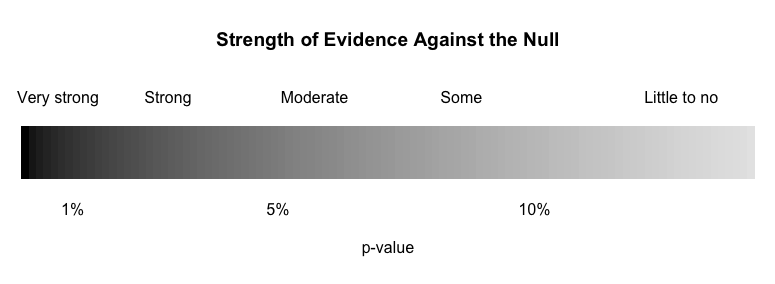
\includegraphics[width=0.9\linewidth]{images/soe_gradient_grayscale} \end{center}

\begin{enumerate}
\def\labelenumi{\arabic{enumi}.}
\setcounter{enumi}{24}
\tightlist
\item
  What does the p-value measure? Interpret the p-value in context of the problem.
\end{enumerate}

\vspace{1in}

\hypertarget{communicate-the-results-and-answer-the-research-question}{%
\subsubsection*{Communicate the results and answer the research question}\label{communicate-the-results-and-answer-the-research-question}}
\addcontentsline{toc}{subsubsection}{Communicate the results and answer the research question}

When we write a conclusion we answer the research question by stating how much evidence there is for the alternative hypothesis.

\begin{enumerate}
\def\labelenumi{\arabic{enumi}.}
\setcounter{enumi}{25}
\tightlist
\item
  Write a conclusion in context of the study.
\end{enumerate}

\vspace{1in}

\hypertarget{take-home-messages-9}{%
\subsection{Take-home messages}\label{take-home-messages-9}}

\begin{enumerate}
\def\labelenumi{\arabic{enumi}.}
\item
  In a hypothesis test we have two competing hypotheses, the null hypothesis and the alternative hypothesis. The null hypothesis represents either a skeptical perspective or a perspective of no difference or no effect. The alternative hypothesis represents a new perspective such as the possibility that there has been a change or that there is a treatment effect in an experiment.
\item
  In a simulation-based test, we create a distribution of possible simulated statistics for our sample if the null hypothesis is true. Then we see if the calculated observed statistic from the data is likely or unlikely to occur when compared to the null distribution.
\item
  The p-value is the probability of the observed statistic occurring or more extreme if the null hypothesis is true. The farther in the tail of the distribution the observed statistic is, the smaller the probability is (smaller the p-value!). The \textbf{smaller} the p-value, the \textbf{more} evidence the statistic provides \textbf{against} the null hypothesis. (Think carefully about why this makes sense!)
\item
  To create one simulated sample on the null distribution for a sample proportion, spin a spinner with probability equal to \(\pi_0\) (the null value), \(n\) times or draw with replacement \(n\) times from a deck of cards created to reflect \(\pi_0\) as the probability of success. Calculate and plot the proportion of successes from the simulated sample.
\end{enumerate}

\hypertarget{additional-notes-8}{%
\subsection{Additional notes}\label{additional-notes-8}}

Use this space to summarize your thoughts and take additional notes on today's activity and material covered.

\newpage

\hypertarget{activity-7b-helper-hinderer-simulation-ci}{%
\section{Activity 7b: Helper-Hinderer --- Simulation CI}\label{activity-7b-helper-hinderer-simulation-ci}}

\setstretch{1}

\hypertarget{learning-objectives-7}{%
\subsection{Learning objectives}\label{learning-objectives-7}}

\begin{itemize}
\item
  Use bootstrapping to find a confidence interval for a single proportion.
\item
  Interpret a confidence interval for a single proportion.
\end{itemize}

\hypertarget{terminology-review-11}{%
\subsection{Terminology review}\label{terminology-review-11}}

In today's activity, we will introduce simulation-based confidence intervals for a single proportion. Some terms covered in this activity are:

\begin{itemize}
\item
  Parameter of interest
\item
  Bootstrapping
\item
  Confidence interval
\end{itemize}

To review these concepts, see Chapter 5 in your textbook, focusing on Sections 5.1 through 5.3.

\hypertarget{helper-hinderer-1}{%
\subsection{Helper-Hinderer}\label{helper-hinderer-1}}

In the last class, we found very strong evidence that the true proportion of infants who will choose the helper character is greater than 0.5. But what is the true proportion of infants who will choose the helper character? We will
use this same study to estimate this parameter of interest.

As a reminder: Do young children know the difference between helpful and unhelpful behavior? A study by Hamblin, Wynn, and Bloom reported in Nature was intended to check young kids' feelings about helpful and non-helpful behavior. Non-verbal infants ages 6 to 10 months were shown short videos with different shapes either helping or hindering the climber. Researchers were hoping to assess: Are infants able to notice and react to helpful or hindering behavior observed in others? In the study, of the 16 infants age 6 to 10 months, 14 chose the \emph{helper} toy and 2 chose the \emph{hinderer} toy.

A \textbf{point estimate} (our observed statistic) provides a single plausible value for a parameter. However, a point estimate is rarely perfect; usually there is some error in the estimate. In addition to supplying a point estimate of a parameter, a next logical step would be to provide a plausible \emph{range} of values for the parameter. This plausible range of values for the population parameter is called an \textbf{interval estimate} or \textbf{confidence interval}.

\hypertarget{activity-intro.}{%
\subsubsection*{Activity intro.}\label{activity-intro.}}
\addcontentsline{toc}{subsubsection}{Activity intro.}

\begin{enumerate}
\def\labelenumi{\arabic{enumi}.}
\tightlist
\item
  What is the value of the point estimate?
\end{enumerate}

\vspace{0.5in}

\begin{enumerate}
\def\labelenumi{\arabic{enumi}.}
\setcounter{enumi}{1}
\tightlist
\item
  If we took another random sample of 16 infants, would we get the exact same point estimate? Explain why or why not.
\end{enumerate}

\vspace{0.5in}

In today's activity, we will use bootstrapping to find a 95\% confidence interval for \(\pi\), the parameter of interest. See Section 5.3.2 to review bootstrapping.

\begin{enumerate}
\def\labelenumi{\arabic{enumi}.}
\setcounter{enumi}{2}
\tightlist
\item
  In your own words, explain the bootstrapping process.
  \vspace{0.5in}
\end{enumerate}

\hypertarget{use-statistical-analysis-methods-to-draw-inferences-from-the-data-1}{%
\subsubsection*{Use statistical analysis methods to draw inferences from the data}\label{use-statistical-analysis-methods-to-draw-inferences-from-the-data-1}}
\addcontentsline{toc}{subsubsection}{Use statistical analysis methods to draw inferences from the data}

\begin{enumerate}
\def\labelenumi{\arabic{enumi}.}
\setcounter{enumi}{3}
\tightlist
\item
  Write out the parameter of interest for this study in words. \textbf{Hint: this is the same as question 7 in Activity 7a.}
\end{enumerate}

\vspace{0.5in}

To use the computer simulation to create a bootstrap distribution, we will need to enter the

\begin{itemize}
\tightlist
\item
  ``sample size'' (the number of observational units or cases in the sample),
\item
  ``number of successes'' (the number of cases that choose the helper character),
\item
  ``number of repetitions'' (the number of samples to be generated), and
\item
  the ``confidence level'' (which level of confidence are we using to create the confidence interval).
\end{itemize}

\begin{enumerate}
\def\labelenumi{\arabic{enumi}.}
\setcounter{enumi}{4}
\tightlist
\item
  What values should be entered for each of the following into the simulation to create the bootstrap distribution of sample proportions to find a 95\% confidence interval?
  \vspace{1mm}
\end{enumerate}

\begin{itemize}
\tightlist
\item
  Sample size:
\end{itemize}

\vspace{.1in}

\begin{itemize}
\tightlist
\item
  Number of successes:
\end{itemize}

\vspace{.1in}

\begin{itemize}
\tightlist
\item
  Number of repetitions:
\end{itemize}

\vspace{.1in}

\begin{itemize}
\tightlist
\item
  Confidence level (as a decimal):
\end{itemize}

\vspace{.1in}

We will use the \texttt{one\_proportion\_bootstrap\_CI()} function in \texttt{R} (in the \texttt{catstats} package) to simulate the bootstrap distribution of sample proportions and calculate a confidence interval. Using the provided \texttt{R} script file, fill in the values/words for each \texttt{xx} with your answers from question 5 in the one proportion bootstrap confidence interval (CI) code to create a bootstrap distribution with 1000 simulations. Then highlight and run lines 1--11.

\begin{Shaded}
\begin{Highlighting}[]
\FunctionTok{one\_proportion\_bootstrap\_CI}\NormalTok{(}\AttributeTok{sample\_size =}\NormalTok{ xx, }\CommentTok{\# Sample size}
                    \AttributeTok{number\_successes =}\NormalTok{ xx, }\CommentTok{\# Observed number of successes}
                    \AttributeTok{number\_repetitions =} \DecValTok{1000}\NormalTok{, }\CommentTok{\# Number of bootstrap samples to use}
                    \AttributeTok{confidence\_level =} \FloatTok{0.95}\NormalTok{) }\CommentTok{\# Confidence level as a decimal}
\end{Highlighting}
\end{Shaded}

\begin{enumerate}
\def\labelenumi{\arabic{enumi}.}
\setcounter{enumi}{5}
\tightlist
\item
  Sketch the bootstrap distribution created below.
\end{enumerate}

\vspace{1.8in}

\begin{enumerate}
\def\labelenumi{\arabic{enumi}.}
\setcounter{enumi}{6}
\item
  What is the value at the center of this bootstrap distribution? Why does this make sense?
  \vspace{.8in}
\item
  Explain why the two vertical lines are at the 2.5th percentile and the 97.5th percentile.
\end{enumerate}

\vspace{.7in}

\begin{enumerate}
\def\labelenumi{\arabic{enumi}.}
\setcounter{enumi}{8}
\tightlist
\item
  Report the 95\% bootstrapped confidence interval for \(\pi\). Use interval notation: (lower value, upper value).
\end{enumerate}

\vspace{0.2in}

\begin{enumerate}
\def\labelenumi{\arabic{enumi}.}
\setcounter{enumi}{9}
\tightlist
\item
  Interpret the 95\% confidence interval in context.
\end{enumerate}

\vspace{.7in}

\hypertarget{communicate-the-results-and-answer-the-research-question-1}{%
\subsubsection*{Communicate the results and answer the research question}\label{communicate-the-results-and-answer-the-research-question-1}}
\addcontentsline{toc}{subsubsection}{Communicate the results and answer the research question}

\begin{enumerate}
\def\labelenumi{\arabic{enumi}.}
\setcounter{enumi}{10}
\tightlist
\item
  Is the value 0.5 (the null value) in the 95\% confidence interval?
\end{enumerate}

\vspace{.2in}

~~~Explain how this indicates that the p-value provides strong evidence against the null.

\newpage

\hypertarget{effect-of-confidence-level}{%
\subsubsection*{Effect of confidence level}\label{effect-of-confidence-level}}
\addcontentsline{toc}{subsubsection}{Effect of confidence level}

\begin{enumerate}
\def\labelenumi{\arabic{enumi}.}
\setcounter{enumi}{11}
\tightlist
\item
  Suppose instead of finding a 95\% confidence interval, we found a 90\% confidence interval. Would you expect the 90\% confidence interval to be narrower or wider? Explain your answer.
\end{enumerate}

\vspace{0.4in}

\begin{enumerate}
\def\labelenumi{\arabic{enumi}.}
\setcounter{enumi}{12}
\tightlist
\item
  The following \texttt{R} code produced the bootstrap distribution with 1000 simulations that follows. Circle the value that changed in the code.
\end{enumerate}

\begin{Shaded}
\begin{Highlighting}[]
\FunctionTok{one\_proportion\_bootstrap\_CI}\NormalTok{(}\AttributeTok{sample\_size =} \DecValTok{16}\NormalTok{, }\CommentTok{\# Sample size}
                    \AttributeTok{number\_successes =} \DecValTok{14}\NormalTok{, }\CommentTok{\# Observed number of successes}
                    \AttributeTok{number\_repetitions =} \DecValTok{1000}\NormalTok{, }\CommentTok{\# Number of bootstrap samples to use}
                    \AttributeTok{confidence\_level =} \FloatTok{0.90}\NormalTok{) }\CommentTok{\# Confidence level as a decimal}
\end{Highlighting}
\end{Shaded}

\begin{center}\includegraphics[width=0.7\linewidth]{07-A10-inference-1cat_CI-simulation_files/figure-latex/unnamed-chunk-2-1} \end{center}

\begin{enumerate}
\def\labelenumi{\arabic{enumi}.}
\setcounter{enumi}{13}
\tightlist
\item
  Report both the 95\% confidence interval (question 9) and the 90\% confidence interval (question 13). Is the 90\% confidence interval narrower or wider than the 95\% confidence interval?
\end{enumerate}

\vspace{0.5in}

\begin{enumerate}
\def\labelenumi{\arabic{enumi}.}
\setcounter{enumi}{14}
\tightlist
\item
  Explain why the upper value of the confidence interval is truncated at 1.
\end{enumerate}

\vspace{0.5in}

\hypertarget{take-home-messages-10}{%
\subsection{Take-home messages}\label{take-home-messages-10}}

\begin{enumerate}
\def\labelenumi{\arabic{enumi}.}
\item
  The goal in a hypothesis test is to assess the strength of evidence for an effect, while the goal in creating a confidence interval is to determine how large the effect is. A \textbf{confidence interval} is a range of \emph{plausible} values for the parameter of interest.
\item
  A confidence interval is built around the point estimate or observed calculated statistic from the sample. This means that the sample statistic is always the center of the confidence interval. A confidence interval includes a measure of sample to sample variability represented by the \textbf{margin of error}.
\item
  In simulation-based methods (bootstrapping), a simulated distribution of possible sample statistics is created showing the possible sample to sample variability. Then we find the middle percent of the distribution around the sample statistic using the percentile method to give the range of values for the confidence interval. This shows us that we are \(X\)\% confident that the parameter is within these values, where \(X\) represents the level of confidence.
\item
  When the null value is within the confidence interval, it is a plausible value for the parameter of interest; thus, we would find a larger p-value for a hypothesis test of that null value. Conversely, if the null value is NOT within the confidence interval, we would find a small p-value for the hypothesis test and strong evidence against this null hypothesis.
\item
  To create one simulated sample on the bootstrap distribution for a sample proportion, label \(n\) cards with the original responses. Draw with replacement \(n\) times. Calculate and plot the resampled proportion of successes.
\end{enumerate}

\hypertarget{additional-notes-9}{%
\subsection{Additional notes}\label{additional-notes-9}}

Use this space to summarize your thoughts and take additional notes on today's activity and material covered.

\newpage

\hypertarget{week-7-lab-comic-book-characters}{%
\section{Week 7 Lab: Comic Book Characters}\label{week-7-lab-comic-book-characters}}

\setstretch{1}

\hypertarget{learning-objectives-8}{%
\subsection{Learning objectives}\label{learning-objectives-8}}

\begin{itemize}
\item
  Identify the two possible explanations (one assuming the null hypothesis, and one assuming the alternative hypothesis) for a relationship seen in sample data.
\item
  Given a research question involving a single categorical variable, construct the null and alternative hypotheses in words and using appropriate statistical symbols.
\item
  Describe and perform a simulation-based hypothesis test for a single proportion.
\item
  Interpret and evaluate a p-value for a simulation-based hypothesis test for a single proportion.
\item
  Use bootstrapping to find a confidence interval for a single proportion.
\item
  Interpret a confidence interval for a single proportion.
\item
  Interpret what confidence means in a confidence interval
\end{itemize}

\hypertarget{comic-book-characters}{%
\subsection{Comic Book Characters}\label{comic-book-characters}}

Among all comic book characters produced by the comic book publisher Marvel, 25\% are female. The comic book publisher DC Comics has taken note of this disparity in the number of female versus male characters, and is trying to diversify their offerings. In a random sample of recently published DC Comics books, 52 characters were included in the comics, of which 15 are female. \textbf{Remember that the bolded questions will be turned in on Gradescope for your group.}

\begin{enumerate}
\def\labelenumi{\arabic{enumi}.}
\tightlist
\item
  What type of plot would be appropriate to display this data?
\end{enumerate}

\vspace{0.3in}

\begin{enumerate}
\def\labelenumi{\arabic{enumi}.}
\setcounter{enumi}{1}
\tightlist
\item
  Calculate the summary statistic. Use appropriate notation.
\end{enumerate}

\vspace{0.3in}

\textbf{3. Write the parameter of interest in context of the problem.}

\vspace{0.8in}

\begin{enumerate}
\def\labelenumi{\arabic{enumi}.}
\setcounter{enumi}{3}
\tightlist
\item
  Write the null hypothesis in notation.
\end{enumerate}

\vspace{0.3in}

\begin{enumerate}
\def\labelenumi{\arabic{enumi}.}
\setcounter{enumi}{4}
\tightlist
\item
  Write the alternative hypothesis in words.
\end{enumerate}

\vspace{0.8in}

\begin{enumerate}
\def\labelenumi{\arabic{enumi}.}
\setcounter{enumi}{5}
\tightlist
\item
  Is the independence condition met? Explain.
\end{enumerate}

\vspace{0.6in}

\begin{enumerate}
\def\labelenumi{\arabic{enumi}.}
\setcounter{enumi}{6}
\tightlist
\item
  What values should be entered for each of the following into the one proportion test to create 1000 simulations?
\end{enumerate}

\vspace{1mm}

\begin{itemize}
\tightlist
\item
  Probability of success:
\end{itemize}

\vspace{.2in}

\begin{itemize}
\tightlist
\item
  Sample size:
\end{itemize}

\vspace{.2in}

\begin{itemize}
\tightlist
\item
  Number of repetitions:
\end{itemize}

\vspace{.2in}

\begin{itemize}
\tightlist
\item
  As extreme as:
\end{itemize}

\vspace{.2in}

\begin{itemize}
\tightlist
\item
  Direction (\texttt{"greater"}, \texttt{"less"}, or \texttt{"two-sided"}):
\end{itemize}

\vspace{.2in}

We will use the \texttt{one\_proportion\_test()} function in \texttt{R} (in the \texttt{catstats} package) to simulate the null distribution of sample proportions and compute a p-value. Using the provided \texttt{R} script file, fill in the values/words for each \texttt{xx} with your answers from question 7 in the one proportion test to create a null distribution with 1000 simulations. Then highlight and run lines 1--10. \textbf{Upload a copy of the created null distribution showing your p-value to Gradescope.}

\begin{Shaded}
\begin{Highlighting}[]
\FunctionTok{one\_proportion\_test}\NormalTok{(}\AttributeTok{probability\_success =}\NormalTok{ xx, }\CommentTok{\# Null hypothesis value}
          \AttributeTok{sample\_size =}\NormalTok{ xx, }\CommentTok{\# Enter sample size}
          \AttributeTok{number\_repetitions =} \DecValTok{1000}\NormalTok{, }\CommentTok{\# Enter number of simulations}
          \AttributeTok{as\_extreme\_as =}\NormalTok{ xx, }\CommentTok{\# Observed statistic}
          \AttributeTok{direction =} \StringTok{"xx"}\NormalTok{, }\CommentTok{\# Specify direction of alternative hypothesis}
          \AttributeTok{report\_value =} \StringTok{"proportion"}\NormalTok{) }\CommentTok{\# Reporting proportion or number of successes?}
\end{Highlighting}
\end{Shaded}

\textbf{8. Report the p-value. Interpret the p-value in context of the study.}

\vspace{1in}

\begin{enumerate}
\def\labelenumi{\arabic{enumi}.}
\setcounter{enumi}{8}
\tightlist
\item
  Write a conclusion in context of the study.
\end{enumerate}

\vspace{1in}

\begin{enumerate}
\def\labelenumi{\arabic{enumi}.}
\setcounter{enumi}{9}
\tightlist
\item
  What values should be entered for each of the following into the simulation to create the bootstrap distribution of sample proportions to find a 95\% confidence interval?
  \vspace{1mm}
\end{enumerate}

\begin{itemize}
\tightlist
\item
  Sample size:
\end{itemize}

\vspace{.1in}

\begin{itemize}
\tightlist
\item
  Number of successes:
\end{itemize}

\vspace{.1in}

\begin{itemize}
\tightlist
\item
  Number of repetitions:
\end{itemize}

\vspace{.1in}

\begin{itemize}
\tightlist
\item
  Confidence level (as a decimal):
\end{itemize}

\vspace{.1in}

We will use the \texttt{one\_proportion\_bootstrap\_CI()} function in \texttt{R} (in the \texttt{catstats} package) to simulate the bootstrap distribution of sample proportions and calculate a confidence interval. Using the provided \texttt{R} script file, fill in the values/words for each \texttt{xx} with your answers from question 10 in the one proportion bootstrap confidence interval (CI) code to create a bootstrap distribution with 1000 simulations. Then highlight and run lines 13--16.

\begin{Shaded}
\begin{Highlighting}[]
\FunctionTok{one\_proportion\_bootstrap\_CI}\NormalTok{(}\AttributeTok{sample\_size =}\NormalTok{ xx, }\CommentTok{\# Sample size}
                    \AttributeTok{number\_successes =}\NormalTok{ xx, }\CommentTok{\# Observed number of successes}
                    \AttributeTok{number\_repetitions =} \DecValTok{1000}\NormalTok{, }\CommentTok{\# Number of bootstrap samples to use}
                    \AttributeTok{confidence\_level =} \FloatTok{0.95}\NormalTok{) }\CommentTok{\# Confidence level as a decimal}
\end{Highlighting}
\end{Shaded}

\begin{enumerate}
\def\labelenumi{\arabic{enumi}.}
\setcounter{enumi}{10}
\tightlist
\item
  Report the 95\% confidence interval.
\end{enumerate}

\vspace{0.5in}

\textbf{12. Interpret the 95\% confidence interval.}

\vspace{0.8in}

\begin{enumerate}
\def\labelenumi{\arabic{enumi}.}
\setcounter{enumi}{12}
\tightlist
\item
  Do the results of the confidence interval agree with the results of the hypothesis test? Explain your answer.
\end{enumerate}

\vspace{0.8in}

\hypertarget{what-does-confidence-mean}{%
\subsection{\texorpdfstring{What does \emph{confidence} mean?}{What does confidence mean?}}\label{what-does-confidence-mean}}

In the interpretation of a 95\% confidence interval, we say that we are 95\% confident that the parameter is within the confidence interval. Why are we able to make that claim? What does it mean to say ``we are 95\% confident?''

\begin{enumerate}
\def\labelenumi{\arabic{enumi}.}
\setcounter{enumi}{13}
\tightlist
\item
  Go to this website, \url{http://www.rossmanchance.com/ISIapplets.html} and choose `Simulating Confidence Intervals.' In the input on the left-hand side of the screen enter 0.25 for \(\pi\), 52 for \(n\), and 100 for `Number of intervals.' Click `sample.'
  \vspace{1mm}
\end{enumerate}

\begin{enumerate}
\def\labelenumi{\alph{enumi}.}
\item
  In the graph on the bottom right, click on a green dot. Write down the confidence interval for this sample given on the graph on the left. Does this confidence interval contain the null value of 0.25?
  \vspace{0.5in}
\item
  Now click on a red dot. Write down the confidence interval for this sample. Does this confidence interval contain the null value of 0.25.?
  \vspace{0.5in}
\item
  How many intervals out of 100 contain \(\pi\), the null value of 0.25? \emph{Hint}: This is given to the left of the graph of green and red intervals.
  \vspace{0.5in}
\end{enumerate}

\begin{enumerate}
\def\labelenumi{\arabic{enumi}.}
\setcounter{enumi}{14}
\tightlist
\item
  Click on `sample' nine more times. Write down the `Running Total' for the proportion of intervals that contain \(\pi\).
\end{enumerate}

\vspace{0.5in}

\textbf{16. Interpret the level of confidence. \emph{Hint}: What proportion of samples would we expect to give a confidence interval that contains the parameter of interest?}

\vspace{0.8in}

\begin{enumerate}
\def\labelenumi{\arabic{enumi}.}
\setcounter{enumi}{16}
\tightlist
\item
  Write a paragraph summarizing the results of the study as if writing a press release. \textbf{Upload your group's paragraph to Gradescope.} Be sure to describe:
\end{enumerate}

\begin{itemize}
\item
  Summary statistic and interpretation
\item
  P-value and interpretation
\item
  Confidence interval and interpretation
\item
  Conclusion (written to answer the research question)
\item
  Scope of inference
\end{itemize}

\newpage

\hypertarget{inference-for-a-single-categorical-variable-theory-based-methods-errors-and-power}{%
\chapter{Inference for a Single Categorical Variable: Theory-based Methods + Errors and Power}\label{inference-for-a-single-categorical-variable-theory-based-methods-errors-and-power}}

\hypertarget{week-7---reading-guide-categorical-inference-1}{%
\section{Week 7 - Reading Guide: Categorical Inference}\label{week-7---reading-guide-categorical-inference-1}}

\hypertarget{section-5.1-foundations-of-inference-hypothesis-tests-1}{%
\subsection*{Section 5.1 (Foundations of inference: Hypothesis tests)}\label{section-5.1-foundations-of-inference-hypothesis-tests-1}}
\addcontentsline{toc}{subsection}{Section 5.1 (Foundations of inference: Hypothesis tests)}

Review section 5.1.2, specifically the notes about the theory-based approach and the Central Limit Theorem.

\hypertarget{section-5.2-the-normal-distribution}{%
\subsection*{Section 5.2 (The normal distribution)}\label{section-5.2-the-normal-distribution}}
\addcontentsline{toc}{subsection}{Section 5.2 (The normal distribution)}

\setstretch{1}

\textbf{Videos}

\begin{itemize}
\tightlist
\item
  5.2
\end{itemize}

\setstretch{1.25}

\hypertarget{vocabulary-12}{%
\subsubsection*{Vocabulary}\label{vocabulary-12}}
\addcontentsline{toc}{subsubsection}{Vocabulary}

Normal distribution (Also known as: normal curve, normal model, Gaussian distribution):
\rgs

\rgi Notation:
\rgs

Standard normal distribution:
\rgs

\rgi Notation:
\rgs

Z-score:
\rgs

\(X\)th percentile:
\rgs

68-95-99.7 rule:
\rgs

\hypertarget{notes-17}{%
\subsubsection*{Notes}\label{notes-17}}
\addcontentsline{toc}{subsubsection}{Notes}

Interpretation of a Z-score:
\rgs

True or False: The more unusual observation will be the observation with the largest Z-score.

Approximately what percent of a normal distribution is in the interval

\rgi (mean -- standard deviation, mean + standard deviation):
\rgs

\rgi (mean -- 2\(\times\)(standard deviation), mean + 2\(\times\)(standard deviation)):
\rgs

\rgi (mean -- 3\(\times\)(standard deviation), mean + 3\(\times\)(standard deviation)):
\rgs

\hypertarget{formulas-1}{%
\subsubsection*{Formulas}\label{formulas-1}}
\addcontentsline{toc}{subsubsection}{Formulas}

Z =
\rgs

\hypertarget{r-coding}{%
\subsection*{\texorpdfstring{\texttt{R} coding}{R coding}}\label{r-coding}}
\addcontentsline{toc}{subsection}{\texttt{R} coding}

\hypertarget{calculating-normal-probabilities}{%
\paragraph*{Calculating normal probabilities}\label{calculating-normal-probabilities}}
\addcontentsline{toc}{paragraph}{Calculating normal probabilities}

When using the \texttt{pnorm()} \texttt{R} function, you will need to enter values for the arguments \texttt{mean}, \texttt{sd}, and \texttt{q} to match the question.

\begin{Shaded}
\begin{Highlighting}[]
\FunctionTok{pnorm}\NormalTok{(}\AttributeTok{mean =}\NormalTok{ mu, }\AttributeTok{sd =}\NormalTok{ sigma, }\AttributeTok{q =}\NormalTok{ x, }\AttributeTok{lower.tail =} \ConstantTok{TRUE}\NormalTok{)}
\end{Highlighting}
\end{Shaded}

This function will return the proportion of the N(\texttt{mu},\texttt{sigma}) distribution which is \emph{below} the value \texttt{x}.

Example: \texttt{pnorm(mean\ =\ 5,\ sd\ =\ 2,\ q\ =\ 3,\ lower.tail\ =\ TRUE)} will give us the proportion of a N(5,2) distribution which is below 3, which equals 0.159:

\begin{Shaded}
\begin{Highlighting}[]
\FunctionTok{pnorm}\NormalTok{(}\AttributeTok{mean =} \DecValTok{5}\NormalTok{, }\AttributeTok{sd =} \DecValTok{2}\NormalTok{, }\AttributeTok{q =} \DecValTok{3}\NormalTok{, }\AttributeTok{lower.tail =} \ConstantTok{TRUE}\NormalTok{)}
\CommentTok{\#\textgreater{} [1] 0.1586553}
\end{Highlighting}
\end{Shaded}

\newpage

Changing to \texttt{lower.tail\ =\ FALSE} will give the proportion of the distribution which is \emph{above} the value \texttt{x}.

\begin{Shaded}
\begin{Highlighting}[]
\FunctionTok{pnorm}\NormalTok{(}\AttributeTok{mean =} \DecValTok{5}\NormalTok{, }\AttributeTok{sd =} \DecValTok{2}\NormalTok{, }\AttributeTok{q =} \DecValTok{3}\NormalTok{, }\AttributeTok{lower.tail =} \ConstantTok{FALSE}\NormalTok{)}
\CommentTok{\#\textgreater{} [1] 0.8413447}
\end{Highlighting}
\end{Shaded}

\hypertarget{displaying-normal-probabilities}{%
\paragraph*{Displaying normal probabilities}\label{displaying-normal-probabilities}}
\addcontentsline{toc}{paragraph}{Displaying normal probabilities}

When using the \texttt{normTail()} \texttt{R} function, you will need to enter values for the arguments \texttt{m}, \texttt{s}, and \texttt{L} (or \texttt{U}) to match the question.

\begin{Shaded}
\begin{Highlighting}[]
\FunctionTok{normTail}\NormalTok{(}\AttributeTok{m =}\NormalTok{ mu, }\AttributeTok{s =}\NormalTok{ sigma, }\AttributeTok{L =}\NormalTok{ x)}
\end{Highlighting}
\end{Shaded}

This function (in the \texttt{openintro} package) will plot a N(\texttt{mu}, \texttt{sigma}) distribution and shade the area that is below the value \texttt{x}.

Example: \texttt{normTail(m\ =\ 5,\ s\ =\ 2,\ L\ =\ 3)} creates the plot pictured below.

\begin{figure}

{\centering 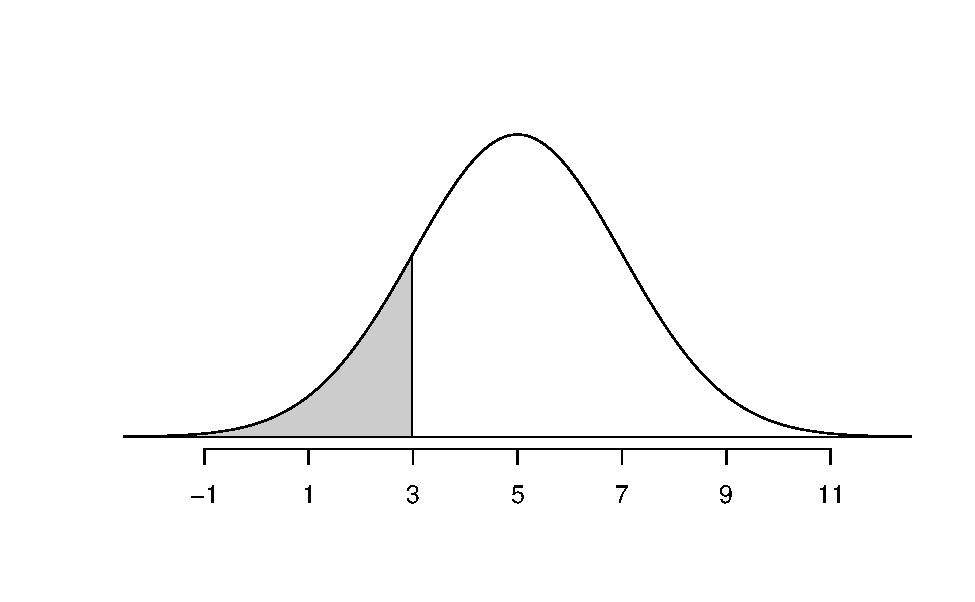
\includegraphics[width=0.6\linewidth]{08-RG-1cat_theory_files/figure-latex/normgt3-1} 

}

\end{figure}

Changing \texttt{L} to \texttt{U} will shade the area \emph{above} \texttt{x}.

Example: \texttt{normTail(m\ =\ 5,\ s\ =\ 2,\ U\ =\ 3)} plots a N(5,2) distribution with the area above 3 shaded.

\hypertarget{calculating-normal-percentiles}{%
\paragraph*{Calculating normal percentiles}\label{calculating-normal-percentiles}}
\addcontentsline{toc}{paragraph}{Calculating normal percentiles}

When using the \texttt{qnorm()} \texttt{R} function, you will need to enter values for the arguments \texttt{mean}, \texttt{sd}, and \texttt{p} to match the question.

\begin{Shaded}
\begin{Highlighting}[]
\FunctionTok{qnorm}\NormalTok{(}\AttributeTok{mean =}\NormalTok{ mu, }\AttributeTok{sd =}\NormalTok{ sigma, }\AttributeTok{p =}\NormalTok{ x, }\AttributeTok{lower.tail =} \ConstantTok{TRUE}\NormalTok{)}
\end{Highlighting}
\end{Shaded}

This function will return the value on the N(\texttt{mu}, \texttt{sigma}) distribution which has \texttt{x} area of the distribution \emph{below} it.

Example: \texttt{qnorm(mean\ =\ 5,\ sd\ =\ 2,\ p\ =\ 0.159,\ lower.tail\ =\ TRUE)} will give us the value on a N(5,2) distribution which has 0.159 (15.9\%) of the distribution below it, which equals 3 (from the \texttt{R} output above).

Changing to \texttt{lower.tail\ =\ FALSE} will give the value which has \texttt{x} area of the distribution \emph{above} it.

We would recommend you work through each of the examples in Section 5.2.4 using \texttt{R}.

\hypertarget{section-5.3.4-theory-based-inferential-methods-for-pi}{%
\subsection*{\texorpdfstring{Section 5.3.4 Theory-based inferential methods for \(\pi\)}{Section 5.3.4 Theory-based inferential methods for \textbackslash pi}}\label{section-5.3.4-theory-based-inferential-methods-for-pi}}
\addcontentsline{toc}{subsection}{Section 5.3.4 Theory-based inferential methods for \(\pi\)}

\setstretch{1}

\textbf{Videos}

\begin{itemize}
\tightlist
\item
  5.3TheoryInf
\end{itemize}

\setstretch{1.25}

\hypertarget{vocabulary-13}{%
\subsubsection*{Vocabulary}\label{vocabulary-13}}
\addcontentsline{toc}{subsubsection}{Vocabulary}

\hypertarget{reminders-from-previous-sections-1}{%
\subsubsection*{Reminders from previous sections}\label{reminders-from-previous-sections-1}}
\addcontentsline{toc}{subsubsection}{Reminders from previous sections}

\(n\) = sample size

\(\hat{p}\) = sample proportion

\(\pi\) = population proportion

General steps of a hypothesis test:

\begin{enumerate}
\def\labelenumi{\arabic{enumi}.}
\item
  Frame the research question in terms of hypotheses.
\item
  Collect and summarize data using a test statistic.
\item
  Assume the null hypothesis is true, and simulate or mathematically model a null distribution for the test statistic.
\item
  Compare the observed test statistic to the null distribution to calculate a p-value.
\item
  Make a conclusion based on the p-value and write the conclusion in context.
\end{enumerate}

Parameter: a value summarizing a variable(s) for a population.

Statistic: a value summarizing a variable(s) for a sample.

Sampling distribution: plot of statistics from 1000s of samples of the same size taken from the same population.

Standard deviation of a statistic: the variability of statistics from 1000s of samples; how far, on average, each statistic is from the true value of the parameter.

Standard error of a statistic: estimated standard deviation of a statistic.

Hypothesis test: a process to determine how strong the evidence of an effect is.

\rgi Also called a `significance test.'

Theory-based method: Develop a mathematical model for the sampling distribution of the statistic under the null hypothesis and use the model to calculate the probability of the observed sample statistic (or one more extreme) occurring.

Null hypothesis (\(H_0\)): the skeptical perspective; no difference; no change; no effect; random chance; what the researcher hopes to prove is \textbf{wrong}.

Alternative hypothesis (\(H_A\)): the new perspective; a difference/increase/decrease; an effect; not random chance; what the researcher hopes to prove is \textbf{correct}.

P-value: probability of seeing the observed sample data, or something more extreme, assuming the null hypothesis is true.

\(\implies\) Lower the p-value the stronger the evidence AGAINST the null hypothesis and FOR the alternative hypothesis.

Decision: a determination of whether to `reject' or `fail to reject' a null hypothesis based on a p-value and a pre-set level of significance.

Significance level (\(\alpha\)): a threshold used to determine if a p-value provides enough evidence to reject the null hypothesis or not.

\rgi Common levels of \(\alpha\) include 0.01, 0.05, and 0.10.

Statistically significant: results are considered statistically significant if the p-value is below the significance level.

Central Limit Theorem: For large sample sizes, the sampling distribution of a sample proportion (or mean) will be approximately normal (bell-shaped and symmetric).

Confidence interval: a process to determine how large an effect is; a range of plausible values for the parameter; also called `estimation.'

Margin of error: the value that is added to and subtracted from the sample statistic to create a confidence interval; half the width of a confidence interval.

\hypertarget{vocabulary-14}{%
\subsubsection*{Vocabulary}\label{vocabulary-14}}
\addcontentsline{toc}{subsubsection}{Vocabulary}

Standardized statistic:
\rgs

Confidence level:
\rgs

\hypertarget{notes-18}{%
\subsubsection*{Notes}\label{notes-18}}
\addcontentsline{toc}{subsubsection}{Notes}

Conditions for the Central Limit Theorem to apply (for the sampling distribution of \(\hat{p}\) to be approximately normal)

\rgi Independence:
\rgs

\rgi \rgi Checked by:
\rgs

\rgi Success-failure condition:
\rgs

\rgi \rgi Checked by:
\rgs

How can we determine the value of \(z^⋆\) to use as the multiplier in a confidence interval?
\rgs

\rgi In \texttt{R}, use \texttt{qnorm(mean\ =\ \_\_,\ sd\ =\ \_\_,\ p\ =\ \_\_)}.

Select one answer in each set of parentheses: The higher the confidence level, the (larger/smaller) the multiplier, meaning the confidence interval will be (wider/narrower).

If the success-failure condition for the Central Limit Theorem is not met, what is the appropriate method of analysis? Select one:
\rgi A. Theory-based approach
\rgi B. Simulation based approach.

\hypertarget{formulas-2}{%
\subsubsection*{Formulas}\label{formulas-2}}
\addcontentsline{toc}{subsubsection}{Formulas}

\(SD(\hat{p})\) =
\rgs

Null standard error of the sample proportion:

\(SE_0(\hat{p})\) =
\rgs

Standardized statistic (in this case, standardized sample proportion):

\(Z\) =
\rgs

Standard error of the sample proportion when we do not assume the null hypothesis is true:

\(SE(\hat{p})\) =
\rgs

Theory-based confidence interval for a sample proportion:
\rgs

Margin of error of a confidence interval for a sample proportion:
\rgs

\hypertarget{example-organ-donations-1}{%
\subsubsection*{Example: Organ donations}\label{example-organ-donations-1}}
\addcontentsline{toc}{subsubsection}{Example: Organ donations}

\begin{enumerate}
\def\labelenumi{\arabic{enumi}.}
\item
  What is the sample statistic presented in this example? What notation would be used to represent this value?
  \rgs
\item
  What is the sample size in this example?
  \rgs
\item
  Are the conditions met to use theoretical methods to analyze these data? Show your calculations to justify your answer.
  \rgs
  \rgs
\end{enumerate}

\hypertarget{example-payday-loans}{%
\subsubsection*{Example: Payday loans}\label{example-payday-loans}}
\addcontentsline{toc}{subsubsection}{Example: Payday loans}

\begin{enumerate}
\def\labelenumi{\arabic{enumi}.}
\item
  What is the parameter representing in the context of this problem? What notation would be used to represent this parameter?
  \rgs
  \rgs
\item
  Write the null and alternative hypotheses in words.
  \rgs
  \rgs
\item
  Write the null and alternative hypotheses in notation.
  \rgs
\item
  Are the conditions met to use theoretical methods to analyze these data? Show your calculations to justify your answer.
  \rgs
  \rgs
\item
  Calculate the null standard error of the sample proportion.
  \rgs
  \rgs
\item
  What is the sample statistic presented in this example? What notation would be used to represent this value?
  \rgs
\item
  Calculate the standardized sample proportion.
  \rgs
  \rgs
\item
  How can we calculate a p-value from the normal distribution for this example?
  \rgs
  \rgs
\item
  What was the p-value of the test?
  \rgs
\item
  At the 5\% significance level, what decision would you make?
  \rgs
\item
  What conclusion should the researcher make?
  \rgs
  \rgs
\item
  Are the results in this example statistically significant? Justify your answer.
  \rgs
\item
  Calculate the standard error of the sample proportion when we do not assume the null hypothesis is true.
  \rgs
  \rgs
\item
  Calculate the margin of error for a 95\% confidence interval for \(\pi\) using 1.96 as the multiplier.
  \rgs
  \rgs
\item
  Calculate a 95\% confidence interval for \(\pi\) using your margin of error calculated above.
  \rgs
  \rgs
\item
  Interpret the 95\% confidence interval provided in the textbook.
  \rgs
  \rgs
\item
  Are the results in this example statistically significant? Justify your answer.
  \rgs
\end{enumerate}

\hypertarget{section-5.5-errors-power-and-practical-importance}{%
\subsection*{Section 5.5 (Errors, power, and practical importance)}\label{section-5.5-errors-power-and-practical-importance}}
\addcontentsline{toc}{subsection}{Section 5.5 (Errors, power, and practical importance)}

\setstretch{1}

\textbf{Videos}

\begin{itemize}
\tightlist
\item
  5.4
\end{itemize}

\setstretch{1.25}

\hypertarget{reminders-from-previous-sections-2}{%
\subsubsection*{Reminders from previous sections}\label{reminders-from-previous-sections-2}}
\addcontentsline{toc}{subsubsection}{Reminders from previous sections}

Decision: a determination of whether to reject or fail to reject a null hypothesis based on a p-value and a pre-set level of significance.

\begin{itemize}
\item
  If p-value \(\leq \alpha\), then reject \(H_0\).
\item
  If p-value \(> \alpha\), then fail to reject \(H_0\).
\end{itemize}

Significance level (\(\alpha\)): a threshold used to determine if a p-value provides enough evidence to reject the null hypothesis or not.

\rgi Common levels of \(\alpha\) include 0.01, 0.05, and 0.10.

Statistically significant: results are considered statistically significant if the p-value is below the significance level.

\hypertarget{vocabulary-15}{%
\subsubsection*{Vocabulary}\label{vocabulary-15}}
\addcontentsline{toc}{subsubsection}{Vocabulary}

Type 1 error:
\rgs

Type 2 error:
\rgs

Confirmation bias:
\rgs

Power:
\rgs

Practical importance:
\rgs

\hypertarget{notes-19}{%
\subsubsection*{Notes}\label{notes-19}}
\addcontentsline{toc}{subsubsection}{Notes}

Fill in the following table with whether the decision was correct or not, and if not, what type of error was made.

\begin{center}
\begin{tabular}{|p{2in}|p{2in}|p{2in}|}
\hline
 & \multicolumn{2}{|c|}{\textbf{Test conclusion (based on data)}} \\ \hline
 \textbf{Truth (unknown)} & Reject null hyp. & Fail to reject null hyp. \\ \hline
 $H_0$ is true && \\ 
   & & \\ 
   & & \\ \hline
 $H_A$ is true ($H_0$ is false)  && \\ 
   & & \\ 
   & & \\ \hline
\end{tabular}
\end{center}

\rgs

How are the significance level and type I error rate related?
\rgs

How are the significance level and type II error rate related?
\rgs

After collecting data, a researcher decides to change from a two-sided test to a one-sided test. Why is this a bad idea?

\begin{enumerate}
\def\labelenumi{\arabic{enumi}.}
\item
  It \_\_\_\_\_\_\_\_\_\_\_\_ (increases/decreases) the chance of a type I error.
\item
  This can result in \_\_\_\_\_\_\_\_\_\_\_\_\_\_\_\_\_\_\_\_\_\_\_\_.
  \rgs
\end{enumerate}

How are power and type I error rate related?
\rgs

How are power and type II error rate related?
\rgs

How can we increase the power of a test?

\begin{enumerate}
\def\labelenumi{\arabic{enumi}.}
\item
  \_\_\_\_\_\_\_\_ (Increase/Decrease) the significance level
  \rgs
\item
  \_\_\_\_\_\_\_\_ (Increase/Decrease) the sample size
  \rgs
\item
  Change from a \_\_\_ (one/two)-sided to a \_\_\_ (one/two)-sided test
  \rgs
\item
  Have a \_\_\_\_\_\_\_\_ (larger/smaller) standard deviation of the statistic
  \rgs
\item
  Have the alternative parameter value \_\_\_\_\_\_\_ (closer/farther) from the null value
  \rgs
\end{enumerate}

Results are likely to be statistically significant (but may not be practically important) if the sample size is \_\_\_\_\_\_\_\_\_\_(large/small).
\rgs

Results are unlikely to be statistically significant (but may be practically important) if the sample size is \_\_\_\_\_\_\_\_\_\_(large/small).
\rgs

\hypertarget{examples}{%
\subsubsection*{Examples:}\label{examples}}
\addcontentsline{toc}{subsubsection}{Examples:}

\begin{enumerate}
\def\labelenumi{\arabic{enumi}.}
\tightlist
\item
  In the Martian Alphabet study in the textbook and presented as an example in Reading Guide 5.1,
\end{enumerate}

\rgi a. What was the p-value of the test?
\rgs

\rgi b. At the 5\% significance level, what decision would you make?
\rgs

\rgi c.~What type of error might have occurred in these data?
\rgs

\rgi d.~Interpret that error in the context of the problem.
\rgs
\rgs

\begin{enumerate}
\def\labelenumi{\arabic{enumi}.}
\setcounter{enumi}{1}
\tightlist
\item
  In the Medical Consultant study in the textbook and presented as an example in the reading guide for sections 5.3.1--5.3.3,
\end{enumerate}

\rgi a. What was the p-value of the test?
\rgs

\rgi b. At the 5\% significance level, what decision would you make?
\rgs

\rgi c.~What type of error might have occurred in these data?
\rgs

\rgi d.~Interpret that error in the context of the problem.
\rgs
\rgs

\begin{enumerate}
\def\labelenumi{\arabic{enumi}.}
\setcounter{enumi}{2}
\tightlist
\item
  In the Payday Loans study in the textbook and presented as an example in the reading guide for section 5.3.4,
\end{enumerate}

\rgi a. What was the p-value of the test?
\rgs

\rgi b. At the 5\% significance level, what decision would you make?
\rgs

\rgi c.~What type of error might have occurred in these data?
\rgs

\rgi d.~Interpret that error in the context of the problem.
\rgs
\rgs

\newpage

\hypertarget{activity-8a-handedness-of-male-boxers-theory-ht}{%
\section{Activity 8a: Handedness of Male Boxers --- Theory HT}\label{activity-8a-handedness-of-male-boxers-theory-ht}}

\setstretch{1}

\hypertarget{learning-objectives-9}{%
\subsection{Learning objectives}\label{learning-objectives-9}}

\begin{itemize}
\item
  Describe and perform a theory-based hypothesis test for a single proportion.
\item
  Check the appropriate conditions to use a theory-based hypothesis test.
\item
  Calculate and interpret the standardized sample proportion.
\item
  Interpret and evaluate a p-value for a theory-based hypothesis test for a single proportion.
\item
  Use the normal distribution to find the p-value.
\end{itemize}

\hypertarget{terminology-review-12}{%
\subsection{Terminology review}\label{terminology-review-12}}

In today's activity, we will introduce theory-based confidence intervals for a single categorical variable. Some terms covered in this activity are:

\begin{itemize}
\item
  Parameter of interest
\item
  Standardized Statistic
\item
  Normal distribution
\item
  p-value
\end{itemize}

To review these concepts, see Chapter 5 in your textbook, focusing on Sections 5.1 through 5.3.

Activity 7a covered simulation-based methods for hypothesis tests involving a single categorical variable. This activity covers theory-based methods for testing a single categorical variable.

Left-handedness is a trait that is found in about 10\% of the general population. Past studies have shown that left-handed men are over-represented among professional boxers. The fighting claim states that left-handed men have an advantage in competition. In this random sample of 500 male professional boxers, we want to see if there is an over-prevalence of left-handed fighters. In the sample of 500 male boxers, 81 were left-handed.

\begin{Shaded}
\begin{Highlighting}[]
 \CommentTok{\# Read in data set}
\NormalTok{boxers }\OtherTok{\textless{}{-}} \FunctionTok{read.csv}\NormalTok{(}\StringTok{"https://math.montana.edu/courses/s216/data/Male\_boxers\_sample.csv"}\NormalTok{)}
\NormalTok{boxers }\SpecialCharTok{\%\textgreater{}\%} \FunctionTok{count}\NormalTok{(Stance)  }\CommentTok{\# Count number in each Stance category}
\end{Highlighting}
\end{Shaded}

\begin{verbatim}
#>         Stance   n
#> 1  left-handed  81
#> 2 right-handed 419
\end{verbatim}

\hypertarget{review-of-summary-stats}{%
\subsection{Review of Summary Stats}\label{review-of-summary-stats}}

\begin{enumerate}
\def\labelenumi{\arabic{enumi}.}
\tightlist
\item
  Write out the parameter of interest for this study.
\end{enumerate}

\vspace{0.8in}

\begin{enumerate}
\def\labelenumi{\arabic{enumi}.}
\setcounter{enumi}{1}
\tightlist
\item
  Give the value of the summary statistic for this study. Use proper notation.
\end{enumerate}

\vspace{0.3in}

\hypertarget{theory-based-methods}{%
\subsection{Theory-based Methods}\label{theory-based-methods}}

The sampling distribution of a single proportion --- how that proportion varies from sample to sample --- can be mathematically modeled using the normal distribution if certain conditions are met.

Conditions for the sampling distribution of \(\hat{p}\) to follow an approximate normal distribution:

\begin{itemize}
\item
  \textbf{Independence}: The sample's observations are independent, e.g., are from a simple random sample. (\emph{Remember}: This also must be true to use simulation methods!)
\item
  \textbf{Success-failure condition}: We \emph{expect} to see at least 10 successes and 10 failures in the sample, \(n\pi≥10\) and \(n(1-\pi)≥10\).
\end{itemize}

\begin{enumerate}
\def\labelenumi{\arabic{enumi}.}
\setcounter{enumi}{2}
\tightlist
\item
  Verify that the independence condition is satisfied.
\end{enumerate}

\vspace{0.5in}

\begin{enumerate}
\def\labelenumi{\arabic{enumi}.}
\setcounter{enumi}{3}
\tightlist
\item
  Is the success-failure condition met to model the data with the normal distribution? Show your work to support your answer. Hint: We don't know the true value of the parameter, \(\pi\), so we use the null value, \(\pi_0\), to check the success-failure condition.
\end{enumerate}

\vspace{1in}

To calculate the standardized statistic we use the general formula

\[
Z = \frac{\text{point estimate} - \text{null value}}{SE_0(\text{point estimate})}.
\]
For a single categorical variable the standardized sample proportion is calculated using

\[
Z = \frac{\hat{p} - \pi_0}{SE_0(\hat{p})},
\]
where the standard error is calculated using the null value:

\[SE_0(\hat{p})=\sqrt{\frac{\pi_0(1-\pi_0)}{n}}\].
\vspace{0.5mm}

\newpage

\begin{enumerate}
\def\labelenumi{\arabic{enumi}.}
\setcounter{enumi}{4}
\tightlist
\item
  Calculate the null standard error of the sample proportion.
\end{enumerate}

\vspace{1in}

\begin{enumerate}
\def\labelenumi{\arabic{enumi}.}
\setcounter{enumi}{5}
\tightlist
\item
  Calculate the standardized sample proportion.
\end{enumerate}

\vspace{1in}

The standardized statistic is used as a ruler to measure how far the sample statistic is from the null value. Essentially, we are converting the sample proportion into a measure of standard errors to compare to the standard normal distribution.

\begin{figure}

{\centering 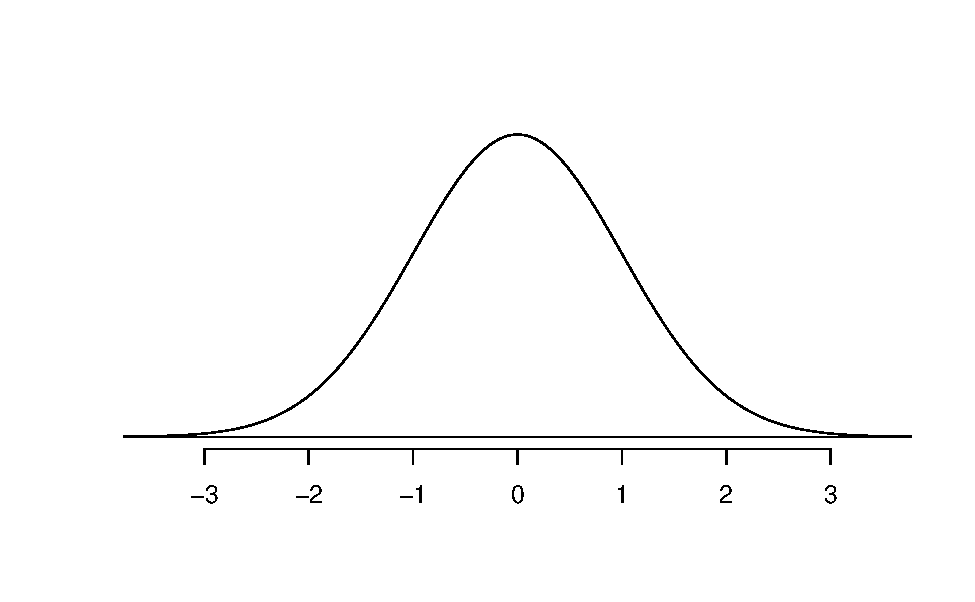
\includegraphics[width=0.6\linewidth]{08-A11-inference-1cat_test-theory_files/figure-latex/simpleNormalcurve-1} 

}

\caption{A standard normal curve.}\label{fig:simpleNormalcurve}
\end{figure}

\begin{enumerate}
\def\labelenumi{\arabic{enumi}.}
\setcounter{enumi}{6}
\tightlist
\item
  Using the 68-95-99.7 rule in Section 5.2.5 to guide you, fill in the percentages on the standard normal distribution displayed in Figure \ref{fig:simpleNormalcurve}, and also mark the value of the standardized statistic calculated in question 6.
\end{enumerate}

\vspace{0.2in}

The standardized statistic measures the \emph{number of standard errors the sample statistic is from the null value}.

\begin{enumerate}
\def\labelenumi{\arabic{enumi}.}
\setcounter{enumi}{7}
\tightlist
\item
  Interpret the standardized sample proportion from question 6 in context of the problem.
\end{enumerate}

\vspace{.8in}

\newpage

We will use the \texttt{pnorm()} function in \texttt{R} to find the p-value. Use the provided \texttt{R} script file and enter the value of the standardized statistic calculated in question 6 at \texttt{xx} in line 7; highlight and run lines 7--9. Notice that in line 9 it says \texttt{lower.tail\ =\ FALSE}. \texttt{R} will calculate the p-value \emph{greater} than the value of the standardized statistic.

Notes:

\begin{itemize}
\tightlist
\item
  Use \texttt{lower.tail\ =\ TRUE} when doing a left-sided test.
\item
  Use \texttt{lower.tail\ =\ FALSE} when doing a right-sided test.
\item
  To find a two-sided p-value, use a left-sided test for negative Z or a right-sided test for positive Z, then multiply the value found by 2 to get the p-value.
\end{itemize}

\begin{Shaded}
\begin{Highlighting}[]
\FunctionTok{pnorm}\NormalTok{(xx, }\CommentTok{\# Enter value of standardized statistic}
      \AttributeTok{m=}\DecValTok{0}\NormalTok{, }\AttributeTok{s=}\DecValTok{1}\NormalTok{, }\CommentTok{\# Using the standard normal mean = 0, sd = 1}
      \AttributeTok{lower.tail=}\ConstantTok{FALSE}\NormalTok{) }\CommentTok{\# Gives a p{-}value greater than the standardized statistic}
\end{Highlighting}
\end{Shaded}

\begin{enumerate}
\def\labelenumi{\arabic{enumi}.}
\setcounter{enumi}{8}
\item
  Report the p-value obtained from the \texttt{R} output.
  \vspace{0.2in}
\item
  Write a conclusion based on the value of the p-value.
  \vspace{0.8in}
\end{enumerate}

\hypertarget{impacts-on-the-p-value}{%
\subsection{Impacts on the P-value}\label{impacts-on-the-p-value}}

Suppose that we want to show that the true proportion of male boxers \textbf{differs} from that in the general population.

\begin{enumerate}
\def\labelenumi{\arabic{enumi}.}
\setcounter{enumi}{10}
\tightlist
\item
  Write out the alternative hypothesis in notation for this new research question.
\end{enumerate}

\vspace{0.5in}

\begin{enumerate}
\def\labelenumi{\arabic{enumi}.}
\setcounter{enumi}{11}
\tightlist
\item
  How would this impact the p-value?
\end{enumerate}

\vspace{0.2in}

\begin{enumerate}
\def\labelenumi{\arabic{enumi}.}
\setcounter{enumi}{12}
\tightlist
\item
  How much evidence would this p-value provide against the null hypothesis?
\end{enumerate}

\vspace{0.3in}

\begin{enumerate}
\def\labelenumi{\arabic{enumi}.}
\setcounter{enumi}{13}
\tightlist
\item
  Suppose instead of 500 male boxers the researchers only took a sample of 300 male boxers and found the same proportion of male boxers that are left-handed. Calculate the standardized statistic for this new sample.
\end{enumerate}

\vspace{1in}

Use Rstudio find the p-value for this new sample. Enter the value of the standardized statistic found in question 14 for xx in line 12. Highlight and run lines 12--14.

\begin{Shaded}
\begin{Highlighting}[]
\FunctionTok{pnorm}\NormalTok{(xx, }\CommentTok{\# Enter value of standardized statistic}
      \AttributeTok{m=}\DecValTok{0}\NormalTok{, }\AttributeTok{s=}\DecValTok{1}\NormalTok{, }\CommentTok{\# Using the standard normal mean = 0, sd = 1}
      \AttributeTok{lower.tail=}\ConstantTok{FALSE}\NormalTok{) }\CommentTok{\# Gives a p{-}value greater than the standardized statistic}
\end{Highlighting}
\end{Shaded}

\begin{enumerate}
\def\labelenumi{\arabic{enumi}.}
\setcounter{enumi}{14}
\tightlist
\item
  How does the decrease in sample size affect the p-value?
\end{enumerate}

\vspace{0.3in}

\begin{enumerate}
\def\labelenumi{\arabic{enumi}.}
\setcounter{enumi}{15}
\tightlist
\item
  Suppose another sample of 500 male boxers was taken and 68 were found to be left-handed. Calculate the standardized statistic for this new sample.
\end{enumerate}

\vspace{1in}

Use Rstudio find the p-value for this new sample.

\begin{Shaded}
\begin{Highlighting}[]
\FunctionTok{pnorm}\NormalTok{(xx, }\CommentTok{\# Enter value of standardized statistic}
      \AttributeTok{m=}\DecValTok{0}\NormalTok{, }\AttributeTok{s=}\DecValTok{1} \CommentTok{\# Using the standard normal mean = 0, sd = 1}
      \AttributeTok{lower.tail=}\ConstantTok{FALSE}\NormalTok{) }\CommentTok{\# Gives a p{-}value greater than the standardized statistic}
\end{Highlighting}
\end{Shaded}

\begin{enumerate}
\def\labelenumi{\arabic{enumi}.}
\setcounter{enumi}{16}
\tightlist
\item
  How does a statistic closer to the null value affect the p-value?
\end{enumerate}

\vspace{0.3in}

\begin{enumerate}
\def\labelenumi{\arabic{enumi}.}
\setcounter{enumi}{17}
\tightlist
\item
  Summarize how each of the following affected the p-value?
\end{enumerate}

\begin{enumerate}
\def\labelenumi{\alph{enumi})}
\tightlist
\item
  Switching to a two-sided test.
\end{enumerate}

\vspace{0.5in}

\begin{enumerate}
\def\labelenumi{\alph{enumi})}
\setcounter{enumi}{1}
\tightlist
\item
  Using a smaller sample size.
\end{enumerate}

\vspace{0.5in}

\begin{enumerate}
\def\labelenumi{\alph{enumi})}
\setcounter{enumi}{2}
\tightlist
\item
  Using a sample statistic closer to the null value.
\end{enumerate}

\vspace{0.5in}

\hypertarget{take-home-messages-11}{%
\subsection{Take-home messages}\label{take-home-messages-11}}

\begin{enumerate}
\def\labelenumi{\arabic{enumi}.}
\item
  Both simulation and theory-based methods can be used to find a p-value for a hypothesis test. In order to use theory-based methods we need to check that both the independence and the success-failure conditions are met.
\item
  The standardized statistic measures how many standard errors the statistic is from the null value. The larger the standardized statistic the more evidence there is against the null hypothesis.
\item
  The p-value for a two-sided test is approximately two times the value for a one-sided test. A two-sided test provides less evidence against the null hypothesis.
\item
  The larger the sample size, the smaller the sample to sample variability. This will result in a larger standardized statistic and more evidence against the null hypothesis.
\item
  The farther the statistic is from the null value, the larger the standardized statistic. This will result in a smaller p-value and more evidence against the null hypothesis.
\end{enumerate}

\hypertarget{additional-notes-10}{%
\subsection{Additional notes}\label{additional-notes-10}}

Use this space to summarize your thoughts and take additional notes on today's activity and material covered.

\newpage

\hypertarget{activity-8b-male-boxers-theory-ci}{%
\section{Activity 8b: Male Boxers --- Theory CI}\label{activity-8b-male-boxers-theory-ci}}

\setstretch{1}

\hypertarget{learning-objectives-10}{%
\subsection{Learning objectives}\label{learning-objectives-10}}

\begin{itemize}
\item
  Calculate a theory-based confidence interval for a single proportion.
\item
  Check the appropriate conditions to find a theory-based confidence interval.
\item
  Interpret a confidence interval for a single proportion.
\item
  Use the normal distribution to find the multiplier needed for a confidence interval
\end{itemize}

\hypertarget{terminology-review-13}{%
\subsection{Terminology review}\label{terminology-review-13}}

In this activity, we will introduce simulation-based confidence intervals for a single proportion. Some terms covered in this activity are:

\begin{itemize}
\item
  Parameter of interest
\item
  Multiplier
\item
  Normal distribution
\end{itemize}

To review these concepts, see Chapter 5 in your textbook, focusing on Sections 5.1 through 5.3.

\hypertarget{male-boxers}{%
\subsection{Male Boxers}\label{male-boxers}}

Last class we found very strong evidence that the true proportion of male boxers that are left-handed is greater than 0.1. In this activity we will use the same data set to find the theory-based 95\% confidence interval.

Remember from the last activity: Left-handedness is a trait that is found in about 10\% of the general population. Past studies have shown that left-handed men are over-represented among professional boxers. The fighting claim states that left-handed men have an advantage in competition. In this random sample of 500 male professional boxers, we want to see if there is an over-prevalence of left-handed fighters. In the sample of 500 male boxers, 81 were left-handed.

Recall that to use theory-based methods we must check the conditions to approximate the sampling distribution with the normal distribution. From the previous activity, we saw that independence was satisfied as the researchers took a random sample.

To check the success-failure condition to use theory-based methods for confidence intervals, we use \(\hat{p}\) in the calculations since we are not assuming a value for \(\pi\). That is, check that we have at least 10 successes and 10 failures in our \textbf{sample}: \(n\hat{p} \geq 0\) and \(n(1-\hat{p}) \geq 10\).

\begin{enumerate}
\def\labelenumi{\arabic{enumi}.}
\tightlist
\item
  Verify that the success-failure condition is met to use theory based methods to find a 95\% confidence interval.
\end{enumerate}

\vspace{0.5in}
\newpage

To calculate a theory-based 95\% confidence interval for \(\pi\), we will first find the \textbf{standard error} of \(\hat{p}\) by plugging in the value of \(\hat{p}\) for \(\pi\) in \(SD(\hat{p})\):

\[SE(\hat{p}) = \sqrt{\frac{\hat{p}(1-\hat{p})}{n}}.\]
Note that we do not include a ``0'' subscript, since we are not assuming a null hypothesis.

\begin{enumerate}
\def\labelenumi{\arabic{enumi}.}
\setcounter{enumi}{1}
\tightlist
\item
  Calculate the standard error of the sample proportion to find a 95\% confidence interval.
\end{enumerate}

\vspace{0.5in}

Recall from earlier in the semester we learned that the sample standard deviation measures the average variability of the data values in the sample from the sample mean. In other words, the sample standard deviation measures how far each data point is from the mean of the data, on average.

\begin{enumerate}
\def\labelenumi{\arabic{enumi}.}
\setcounter{enumi}{2}
\tightlist
\item
  Interpret the standard error of the sample proportion found in question 2 in context of the problem.
\end{enumerate}

\vspace{0.8in}

To find the confidence interval, we will add and subtract the \textbf{margin of error} to the point estimate:

\[\text{point estimate}\pm\text{margin of error}\]
\[\hat{p}\pm z^* SE(\hat{p})\]

The \(z^*\) multiplier is the percentile of a standard normal distribution that corresponds to our confidence level. If our confidence level is 95\%, we find the Z values that encompass the middle 95\% of the standard normal distribution. If 95\% of the standard normal distribution should be in the middle, that leaves 5\% in the tails, or 2.5\% in each tail. The \texttt{qnorm()} function in \texttt{R} will tell us the \(z^*\) value for the desired percentile (in this case, 95\% + 2.5\% = 97.5\% percentile).

\begin{Shaded}
\begin{Highlighting}[]
\FunctionTok{qnorm}\NormalTok{(}\FloatTok{0.975}\NormalTok{) }\CommentTok{\# Multiplier for 95\% confidence interval}
\end{Highlighting}
\end{Shaded}

\begin{verbatim}
#> [1] 1.959964
\end{verbatim}

\begin{figure}

{\centering 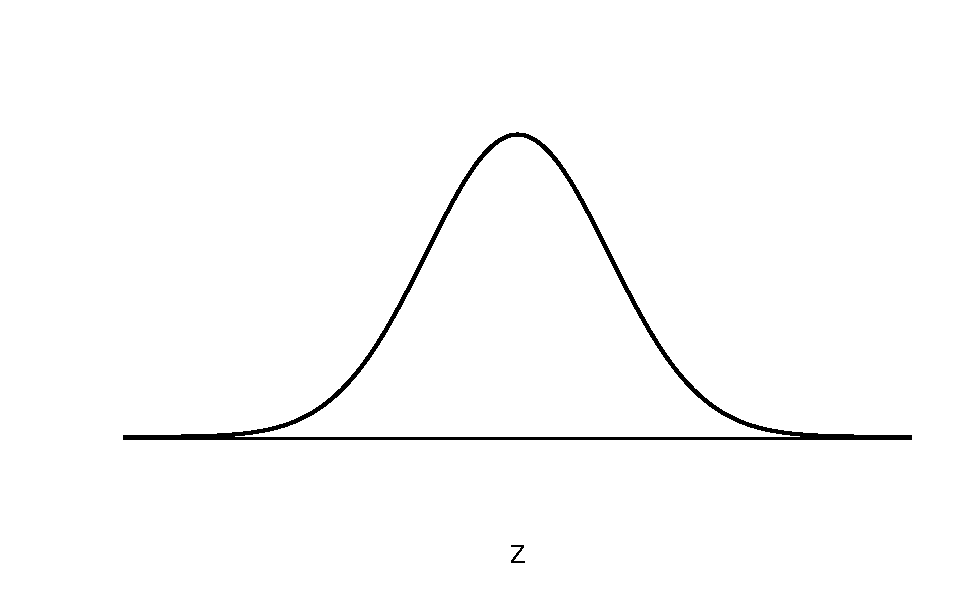
\includegraphics[width=0.6\linewidth]{08-A12-inference-1cat_CI-theory_files/figure-latex/simpleNormaldist-1} 

}

\caption{A standard normal curve.}\label{fig:simpleNormaldist}
\end{figure}

\begin{enumerate}
\def\labelenumi{\arabic{enumi}.}
\setcounter{enumi}{3}
\tightlist
\item
  Fill in the normal distribution above to show how \texttt{R} found the \(z^*\) multiplier.
\end{enumerate}

\vspace{0.1in}

\begin{enumerate}
\def\labelenumi{\arabic{enumi}.}
\setcounter{enumi}{4}
\tightlist
\item
  What is the value of the multiplier needed to calculate the 95\% confidence interval for the true proportion of male boxers that are left-handed?
\end{enumerate}

\vspace{1in}

\begin{enumerate}
\def\labelenumi{\arabic{enumi}.}
\setcounter{enumi}{5}
\tightlist
\item
  Calculate the margin of error for the 95\% confidence interval.
\end{enumerate}

\vspace{1in}

\begin{enumerate}
\def\labelenumi{\arabic{enumi}.}
\setcounter{enumi}{6}
\tightlist
\item
  Calculate the 95\% confidence interval for the parameter of interest.
\end{enumerate}

\vspace{0.5in}

\begin{enumerate}
\def\labelenumi{\arabic{enumi}.}
\setcounter{enumi}{7}
\tightlist
\item
  Interpret the 95\% confidence interval in the context of the problem.
\end{enumerate}

\vspace{1in}

\begin{enumerate}
\def\labelenumi{\arabic{enumi}.}
\setcounter{enumi}{8}
\tightlist
\item
  Is the null value, 0.1, contained in the 95\% confidence interval? Explain, based on the p-value from the last activity, why you expected this to be true.
  \vspace{1in}
\end{enumerate}

\hypertarget{simulation-methods}{%
\subsection*{Simulation Methods}\label{simulation-methods}}
\addcontentsline{toc}{subsection}{Simulation Methods}

In question 1, we found that the success-failure condition was met to use theory-based methods. Here we will use simulation methods to find a 95\% confidence interval for the parameter of interest.

Use the \texttt{one\_proportion\_bootstrap\_CI()} function in \texttt{R} to simulate the bootstrap distribution of sample proportions and calculate a confidence interval. Using the provided \texttt{R} script file, fill in the values/words for each \texttt{xx} in the one proportion bootstrap confidence interval (CI) code to create a bootstrap distribution with 1000 simulations.

\begin{Shaded}
\begin{Highlighting}[]
\FunctionTok{one\_proportion\_bootstrap\_CI}\NormalTok{(}\AttributeTok{sample\_size =}\NormalTok{ xx, }\CommentTok{\# Sample size}
                    \AttributeTok{number\_successes =}\NormalTok{ xx, }\CommentTok{\# Observed number of successes}
                    \AttributeTok{number\_repetitions =} \DecValTok{1000}\NormalTok{, }\CommentTok{\# Number of bootstrap samples to use}
                    \AttributeTok{confidence\_level =} \FloatTok{0.95}\NormalTok{) }\CommentTok{\# Confidence level as a decimal}
\end{Highlighting}
\end{Shaded}

\begin{enumerate}
\def\labelenumi{\arabic{enumi}.}
\setcounter{enumi}{9}
\tightlist
\item
  Report the simulation 95\% confidence interval. Is this confidence interval similar to the confidence interval calculated in question 7?
\end{enumerate}

\vspace{0.8in}

\hypertarget{effect-of-sample-size-1}{%
\subsection*{Effect of Sample Size}\label{effect-of-sample-size-1}}
\addcontentsline{toc}{subsection}{Effect of Sample Size}

Suppose in another sample of 230 male boxers we saw that 37 were left-handed.

\begin{enumerate}
\def\labelenumi{\arabic{enumi}.}
\setcounter{enumi}{10}
\tightlist
\item
  Calculate the margin of error for a 95\% confidence interval using a multiplier \(z^* = 1.96\) for this sample. Is the margin of error larger or smaller than the margin of error for the original study?
\end{enumerate}

\vspace{0.5in}

\begin{enumerate}
\def\labelenumi{\arabic{enumi}.}
\setcounter{enumi}{11}
\tightlist
\item
  Calculate the 95\% confidence interval for this new study using the margin of error from question 11.
\end{enumerate}

\vspace{0.5in}

\begin{enumerate}
\def\labelenumi{\arabic{enumi}.}
\setcounter{enumi}{12}
\tightlist
\item
  Is the confidence interval calculated in question 11 with the smaller sample size wider or smaller than the confidence interval in question 6? Explain your answer
  \vspace{1in}
\end{enumerate}

\hypertarget{take-home-messages-12}{%
\subsection{Take-home messages}\label{take-home-messages-12}}

\begin{enumerate}
\def\labelenumi{\arabic{enumi}.}
\item
  In theory-based methods, we add and subtract a margin of error to the sample statistic. The margin of error is calculated using a multiplier that corresponds to the level of confidence times the variability (standard error) of the statistic.
\item
  The confidence interval calculated using theory-based methods should be similar to the confidence interval found using simulation methods provided the success-failure condition is met.
\item
  A smaller sample size will increase the margin of error which results in a wider confidence interval.
\end{enumerate}

\hypertarget{additional-notes-11}{%
\subsection{Additional notes}\label{additional-notes-11}}

Use this space to summarize your thoughts and take additional notes on today's activity and material covered.

\newpage

\hypertarget{week-8-lab-one-categorical-theory}{%
\section{Week 8 Lab: One-categorical Theory}\label{week-8-lab-one-categorical-theory}}

\setstretch{1}

\hypertarget{learning-objectives-11}{%
\subsection{Learning objectives}\label{learning-objectives-11}}

???

\begin{enumerate}
\def\labelenumi{\arabic{enumi}.}
\setcounter{enumi}{8}
\tightlist
\item
  Is the validity condition met to use theory-based methods to analyze? Explain.
\end{enumerate}

\vspace{0.8in}

\begin{enumerate}
\def\labelenumi{\arabic{enumi}.}
\setcounter{enumi}{9}
\tightlist
\item
  Calculate the standardized statistic.
\end{enumerate}

\vspace{0.8in}

\begin{enumerate}
\def\labelenumi{\arabic{enumi}.}
\setcounter{enumi}{10}
\tightlist
\item
  Interpret the standardized statistic.
\end{enumerate}

\vspace{0.8in}

\begin{enumerate}
\def\labelenumi{\arabic{enumi}.}
\setcounter{enumi}{11}
\tightlist
\item
  Sketch a graph of the normal distribution and how to find the p-value for the theory-based test.
\end{enumerate}

\vspace{1.4in}

Use the following code to find the theory-based p-value.

\begin{Shaded}
\begin{Highlighting}[]
\FunctionTok{pnorm}\NormalTok{(xx, }\CommentTok{\# Enter value of standardized statistic}
      \AttributeTok{m=}\DecValTok{0}\NormalTok{, }\AttributeTok{s=}\DecValTok{1} \CommentTok{\# Using the standard normal mean = 0, sd = 1}
      \AttributeTok{lower.tail=}\ConstantTok{FALSE}\NormalTok{) }\CommentTok{\# Gives a p{-}value greater than the standardized statistic}
\end{Highlighting}
\end{Shaded}

\begin{enumerate}
\def\labelenumi{\arabic{enumi}.}
\setcounter{enumi}{12}
\tightlist
\item
  Why did you expect that the value of the p-value is similar between theory and simulation methods?
\end{enumerate}

\newpage

\hypertarget{inference-for-two-categorical-variables-simulation-based-methods}{%
\chapter{Inference for Two Categorical Variables: Simulation-based Methods}\label{inference-for-two-categorical-variables-simulation-based-methods}}

\hypertarget{week-9---reading-guide-hypothesis-testing-for-a-difference-in-proportions}{%
\section{Week 9 - Reading Guide: Hypothesis Testing for a Difference in Proportions}\label{week-9---reading-guide-hypothesis-testing-for-a-difference-in-proportions}}

\hypertarget{section-5.5-simulation-based-fnference-for-a-difference-in-proportions}{%
\subsection*{Section 5.5 (Simulation-based fnference for a difference in proportions)}\label{section-5.5-simulation-based-fnference-for-a-difference-in-proportions}}
\addcontentsline{toc}{subsection}{Section 5.5 (Simulation-based fnference for a difference in proportions)}

You may skip section 5.5.3, which will be covered next week.

\textbf{Videos}

\begin{itemize}
\tightlist
\item
  5.5SimInf
\end{itemize}

\setstretch{1.25}

\hypertarget{reminders-from-previous-sections-3}{%
\subsubsection*{Reminders from previous sections}\label{reminders-from-previous-sections-3}}
\addcontentsline{toc}{subsubsection}{Reminders from previous sections}

\(n\) = sample size

\(\hat{p}\) = sample proportion

\(\pi\) = population proportion

General steps of a hypothesis test:

\begin{enumerate}
\def\labelenumi{\arabic{enumi}.}
\item
  Frame the research question in terms of hypotheses.
\item
  Collect and summarize data using a test statistic.
\item
  Assume the null hypothesis is true, and simulate or mathematically model a null distribution for the test statistic.
\item
  Compare the observed test (standardized) statistic to the null distribution to calculate a p-value.
\item
  Make a conclusion based on the p-value and write the conclusion in context.
\end{enumerate}

Parameter: a value summarizing a variable(s) for a population.

Statistic: a value summarizing a variable(s) for a sample.

Sampling distribution: plot of statistics from 1000s of samples of the same size taken from the same population.

Standard deviation of a statistic: the variability of statistics from 1000s of samples; how far, on average, each statistic is from the true value of the parameter.

Standard error of a statistic: estimated standard deviation of a statistic.

Hypothesis test: a process to determine how strong the evidence of an effect is.

\rgi Also called a `significance test.'

Simulation-based method: Simulate lots of samples of size \(n\) under assumption of the null hypothesis, then find the proportion of the simulations that are at least as extreme as the observed sample statistic.

Null hypothesis (\(H_0\)): the skeptical perspective; no difference; no change; no effect; random chance; what the researcher hopes to prove is \textbf{wrong}.

Alternative hypothesis (\(H_A\)): the new perspective; a difference/increase/decrease; an effect; not random chance; what the researcher hopes to prove is \textbf{correct}.

Null value: the value of the parameter when we assume the null hypothesis is true (labeled as \(parameter_0\)).

Null distribution: the simulated or modeled distribution of statistics (sampling distribution) we would expect to occur if the null hypothesis is true.

P-value: probability of seeing the observed sample data, or something more extreme, assuming the null hypothesis is true.

\(\implies\) Lower the p-value the stronger the evidence AGAINST the null hypothesis and FOR the alternative hypothesis.

Decision: a determination of whether to `reject' or `fail to reject' a null hypothesis based on a p-value and a pre-set level of significance.

Significance level (\(\alpha\)): a threshold used to determine if a p-value provides enough evidence to reject the null hypothesis or not.

\rgi Common levels of \(\alpha\) include 0.01, 0.05, and 0.10.

Statistically significant: results are considered statistically significant if the p-value is below the significance level.

Confidence interval: a process to determine how large an effect is; a range of plausible values for the parameter. Also called `estimation.'

Margin of error: the value that is added to and subtracted from the sample statistic to create a confidence interval; half the width of a confidence interval.

Bootstrapping: the process of drawing with replacement \(n\) times from the original sample.

Bootstrapped resample: a random sample of size \(n\) from the original sample, selected with replacement.

Bootstrapped statistic: the statistic recorded from the bootstrapped resample.

Confidence level: how confident we are that the confidence interval will capture the parameter.

\hypertarget{vocabulary-16}{%
\subsubsection*{Vocabulary}\label{vocabulary-16}}
\addcontentsline{toc}{subsubsection}{Vocabulary}

Randomization test:
\rgs

Relative risk:
\rgs

\hypertarget{notes-20}{%
\subsubsection*{Notes}\label{notes-20}}
\addcontentsline{toc}{subsubsection}{Notes}

In a randomization test involving two categorical variables, how many cards will you need and how will the cards be labeled?
\rgs

Why, in the randomization test, are the cards all shuffled together and randomly dealt into two new groups?
\rgs

After shuffling, how many cards are dealt into each pile?
\rgs

Interpreting relative risk (\(RR = \frac{\hat{p_1}}{\hat{p_2}}\))

\rgi The proportion of success in group 1 is \_\_\_\_\_\_ times the proportion of success in group 2.

\rgi The proportion of success in group 1 is \_\_\_\_\_\_ \% higher/lower than in group 2.

Write the null hypothesis in notation for a test of relative risk.
\rgs

To create a single bootstrap resample for two categorical variables, how many cards will you need and how will the cards be labeled?
\rgs

What is done with the cards once they are labeled?
\rgs

Interpretations of confidence level must include:
\rgs
\rgs

How do you determine if the results of a hypothesis test agree with a confidence interval?
\rgs
\rgs

How are the confidence level and the significance level related (for a two-sided test)?
\rgs

\hypertarget{formulas-3}{%
\subsubsection*{Formulas}\label{formulas-3}}
\addcontentsline{toc}{subsubsection}{Formulas}

Relative risk =
\rgs

\hypertarget{notation}{%
\subsubsection*{Notation}\label{notation}}
\addcontentsline{toc}{subsubsection}{Notation}

Sample size of group 1:
\rgs

Sample size of group 2:
\rgs

Sample proportion of group 1:
\rgs

Sample proportion of group 2:
\rgs

Population proportion of group 1:
\rgs

Population proportion of group 2:
\rgs

\hypertarget{example-gender-discrimination}{%
\subsubsection*{Example: Gender discrimination}\label{example-gender-discrimination}}
\addcontentsline{toc}{subsubsection}{Example: Gender discrimination}

\begin{enumerate}
\def\labelenumi{\arabic{enumi}.}
\item
  What is the research question?
  \rgs
\item
  What are the observational units?
  \rgs
\item
  What type of study design was used? Justify your answer.
  \rgs
\item
  What is the appropriate scope of inference for these data?
  \rgs
\item
  What is the sample statistic presented in this example? What notation would be used to represent this value?
  \rgs
\item
  What is the parameter representing in the context of this problem? What notation would be used to represent this parameter?
  \rgs
  \rgs
\item
  Write the null and the alternative hypotheses in words.
  \rgs
  \rgs
\item
  Write the null and the alternative hypotheses in notation.
  \rgs
\item
  How could we use cards to simulate \textbf{ome} sample \emph{which assumes the null hypothesis is true}? How many blue cards --- to represent what? How many red cards --- to represent what? What would we do with the cards? What would you record once you have a simulated sample?
  \rgs
  \rgs
  \rgs
\item
  How can we calculate a p-value from the simulated null distribution for this example?
  \rgs
  \rgs
\item
  What was the p-value of the test?
  \rgs
\item
  At the 5\% significance level, what decision would you make?
  \rgs
\item
  What conclusion should the researcher make?
  \rgs
  \rgs
\item
  Are the results in this example statistically significant? Justify your answer.
  \rgs
\end{enumerate}

\hypertarget{example-opportunity-cost}{%
\subsubsection*{Example: Opportunity cost}\label{example-opportunity-cost}}
\addcontentsline{toc}{subsubsection}{Example: Opportunity cost}

\begin{enumerate}
\def\labelenumi{\arabic{enumi}.}
\item
  What is the research question?
  \rgs
\item
  What are the observational units?
  \rgs
\item
  What type of study design was used? Justify your answer.
  \rgs
\item
  What is the appropriate scope of inference for these data?
  \rgs
\item
  What is the sample statistic presented in this example? What notation would be used to represent this value?
  \rgs
\item
  What is the parameter representing in the context of this problem? What notation would be used to represent this parameter?
  \rgs
  \rgs
\item
  Write the null and the alternative hypotheses in words.
  \rgs
  \rgs
\item
  Write the null and the alternative hypotheses in notation.
  \rgs
\item
  How could we use cards to simulate \textbf{one} sample \emph{which assumes the null hypothesis is true}? How many blue cards --- to represent what? How many red cards --- to represent what? What would we do with the cards? What would you record once you have a simulated sample?
  \rgs
  \rgs
  \rgs
\item
  How can we calculate a p-value from the simulated null distribution for this example?
  \rgs
  \rgs
\item
  What was the p-value of the test?
  \rgs
\item
  Interpret the p-value in the context of the problem.
  \rgs
  \rgs
\item
  At the 5\% significance level, what decision would you make?
  \rgs
\item
  What conclusion should the researcher make?
  \rgs
\item
  Are the results in this example statistically significant? Justify your answer.
  \rgs
\end{enumerate}

\hypertarget{example-cpr-and-blood-thinner}{%
\subsubsection*{Example: CPR and blood thinner}\label{example-cpr-and-blood-thinner}}
\addcontentsline{toc}{subsubsection}{Example: CPR and blood thinner}

\begin{enumerate}
\def\labelenumi{\arabic{enumi}.}
\item
  What is the research question?
  \rgs
\item
  What are the observational units?
  \rgs
\item
  What type of study design was used? Justify your answer.
  \rgs
\item
  What is the appropriate scope of inference for these data?
  \rgs
\item
  What is the sample difference in proportions presented in this example? What notation would be used to represent this value?
  \rgs
\item
  What is the sample relative risk? Interpret the value in the context of the study.
  \rgs
  \rgs
\item
  What is the parameter (using a difference in proportion) representing in the context of this problem? What notation would be used to represent this parameter?
  \rgs
  \rgs
\item
  Write the null and the alternative hypotheses in words.
  \rgs
  \rgs
\item
  Write the null and the alternative hypotheses in notation.
  \rgs
\item
  How could we use cards to simulate \textbf{one} sample \emph{which assumes the null hypothesis is true}? How many blue cards --- to represent what? How many red cards --- to represent what? What would we do with the cards? What would you record once you have a simulated sample?
  \rgs
  \rgs
  \rgs
\item
  How can we calculate a p-value from the simulated null distribution for this example?
  \rgs
  \rgs
\item
  What was the p-value of the test?
  \rgs
\item
  Interpret the p-value in the context of the problem.
  \rgs
  \rgs
\item
  At the 5\% significance level, what decision would you make?
  \rgs
\item
  What conclusion should the researcher make?
  \rgs
  \rgs
\item
  Are the results in this example statistically significant? Justify your answer.
  \rgs
\item
  How could we use cards to simulate \textbf{one} bootstrap resample? How many blue cards --- to represent what? How many red cards --- to represent what? What would we do with the cards? What would you record once you have a simulated sample?
  \rgs
  \rgs
  \rgs
\item
  How can we calculate a 90\% confidence interval from the bootstrap distribution for this example?
  \rgs
\item
  What was the 90\% confidence interval?
  \rgs
\item
  Interpret the confidence \emph{interval} in the context of the problem.
  \rgs
  \rgs
\item
  Interpret the confidence \emph{level} in the context of the problem.
  \rgs
  \rgs
\item
  Does the conclusion of the hypothesis test match the confidence interval?
  \rgs
\end{enumerate}

\newpage

\hypertarget{activity-9a-the-good-samaritan-simulation-ht}{%
\section{Activity 9a: The Good Samaritan --- Simulation HT}\label{activity-9a-the-good-samaritan-simulation-ht}}

\setstretch{1}

\hypertarget{learning-objectives-12}{%
\subsection{Learning objectives}\label{learning-objectives-12}}

\begin{itemize}
\item
  Given a research question involving two categorical variables, construct the null and alternative hypotheses
  in words and using appropriate statistical symbols.
\item
  Describe and perform a simulation-based hypothesis test for a difference in proportions.
\item
  Interpret and evaluate a p-value for a simulation-based hypothesis test for a difference in proportions.
\end{itemize}

\hypertarget{terminology-review-14}{%
\subsection{Terminology review}\label{terminology-review-14}}

In today's activity, we will use simulation-based methods to analyze two categorical variables. Some terms covered in this activity are:

\begin{itemize}
\item
  Conditional proportion
\item
  Null hypothesis
\item
  Alternative hypothesis
\end{itemize}

To review these concepts, see Chapter 5 in your textbook.

\hypertarget{the-good-samaritan}{%
\subsection{The Good Samaritan}\label{the-good-samaritan}}

Researchers at the Princeton University wanted to investigate influences on behavior. The researchers randomly selected 67 students from the Princeton Theological Seminary to participate in a study. Only 47 students chose to participate in the study, and the data below includes 40 of those students (7 students were removed from the study for various reasons). As all participants were theology majors planning a career as a preacher, the expectation was that all would have a similar disposition when it comes to helping behavior. Each student was then shown a 5-minute presentation on the Good Samaritan, a parable in the Bible which emphasizes the importance of helping others. After the presentation, the students were told they needed to give a talk on the Good Samaritan parable at a building across campus. Half the students were told they were late for the presentation; the other half told they could take their time getting across campus (the condition was randomly assigned). On the way between buildings, an actor pretending to be a homeless person in distress asked the student for help. The researchers recorded whether the student helped the actor or not. The results of the study are shown in the table below. Do these data provide evidence that those in a hurry will be less likely to help people in need in this situation? Use the order of subtraction hurry -- no hurry.

\begin{longtable}[]{@{}llll@{}}
\toprule
& Hurry Condition & No Hurry Condition & Total \\
\midrule
\endhead
Helped Actor & 2 & 11 & 13 \\
Did Not Help Actor & 18 & 9 & 27 \\
Total & 20 & 20 & 40 \\
\bottomrule
\end{longtable}

\newpage

These counts can be found in \texttt{R} by using the \texttt{count()} function:

\begin{Shaded}
\begin{Highlighting}[]
\CommentTok{\# Read data set in}
\NormalTok{good }\OtherTok{\textless{}{-}} \FunctionTok{read.csv}\NormalTok{(}\StringTok{"data/goodsam.csv"}\NormalTok{) }
\NormalTok{good }\SpecialCharTok{\%\textgreater{}\%} \FunctionTok{group\_by}\NormalTok{(Behavior) }\SpecialCharTok{\%\textgreater{}\%} \FunctionTok{count}\NormalTok{(Condition)}
\end{Highlighting}
\end{Shaded}

\begin{verbatim}
#> # A tibble: 4 x 3
#> # Groups:   Behavior [2]
#>   Behavior Condition     n
#>   <chr>    <chr>     <int>
#> 1 Help     Hurry         2
#> 2 Help     No hurry     11
#> 3 No help  Hurry        18
#> 4 No help  No hurry      9
\end{verbatim}

\hypertarget{vocabulary-review.-2}{%
\subsubsection*{Vocabulary review.}\label{vocabulary-review.-2}}
\addcontentsline{toc}{subsubsection}{Vocabulary review.}

\begin{enumerate}
\def\labelenumi{\arabic{enumi}.}
\tightlist
\item
  What is the name of the explanatory variable in the \texttt{R} output? What are its categories?
\end{enumerate}

\vspace{0.2in}

\begin{enumerate}
\def\labelenumi{\arabic{enumi}.}
\setcounter{enumi}{1}
\tightlist
\item
  What is the response variable in the \texttt{R} output? What are its categories?
\end{enumerate}

\vspace{0.2in}

\setstretch{1.5}

\begin{enumerate}
\def\labelenumi{\arabic{enumi}.}
\setcounter{enumi}{2}
\tightlist
\item
  Fill in the blanks with one answer from each set of parentheses: This is an\\
  \_\_\_\_\_\_\_\_\_\_\_\_\_\_\_\_ (experiment/observational study) because\\
  \_\_\_\_\_\_\_\_\_\_\_\_\_\_ (hurry or no hurry/help or no help) \_\_\_\_\_\_\_ (was/was not)\\
  randomly \_\_\_\_\_\_\_\_\_\_\_\_ (assigned/selected).
\end{enumerate}

\vspace{0.1in}

\begin{enumerate}
\def\labelenumi{\arabic{enumi}.}
\setcounter{enumi}{3}
\tightlist
\item
  Put an X in the box that represents the appropriate scope of inference for this study.
\end{enumerate}

\begin{longtable}[]{@{}cccl@{}}
\toprule
& & Study Type & \\
\midrule
\endhead
& & Randomized Experiment & Observational Study \\
Selection of Cases & Random Sample & & \\
& No Random Sample & & \\
\bottomrule
\end{longtable}

\setstretch{1}

\hypertarget{ask-a-research-question-1}{%
\subsubsection*{Ask a research question}\label{ask-a-research-question-1}}
\addcontentsline{toc}{subsubsection}{Ask a research question}

The research question as stated above is: Do these data provide evidence that those in a hurry will be less likely to help people in need in this situation? In order to set up our hypotheses, we need to express this research question in terms of parameters.

Remember, we define the parameter for a single categorical variable as the true proportion of observational units that are labeled as a ``success'' in the response variable.

\newpage

\begin{enumerate}
\def\labelenumi{\arabic{enumi}.}
\setcounter{enumi}{4}
\item
  Write the two parameters of interest for this study. Let 1 = hurry condition, 2 = no hurry condition.
  \vspace{1mm}

  \(\pi_1\) ---
  \vspace{0.5in}

  \(\pi_2\) ---
  \vspace{0.5in}
\end{enumerate}

When comparing two groups, we assume the two parameters are equal in the null hypothesis---there is no association between the variables.

\begin{enumerate}
\def\labelenumi{\arabic{enumi}.}
\setcounter{enumi}{5}
\tightlist
\item
  Write the null hypothesis out in words using your answers to question 5.
\end{enumerate}

\vspace{0.8in}

\begin{enumerate}
\def\labelenumi{\arabic{enumi}.}
\setcounter{enumi}{6}
\tightlist
\item
  Based on the research question, fill in the appropriate sign for the alternative hypothesis (\(<\), \(>\), or \(\neq\)):
  \vspace{0.1in}
\end{enumerate}

~~~~~~~~~~\(H_A: \pi_1 -\pi_2\) \_\_\_\_\_\_\_\_\_\_ 0

\hypertarget{summarize-and-visualize-the-data-1}{%
\subsubsection*{Summarize and visualize the data}\label{summarize-and-visualize-the-data-1}}
\addcontentsline{toc}{subsubsection}{Summarize and visualize the data}

\begin{enumerate}
\def\labelenumi{\arabic{enumi}.}
\setcounter{enumi}{7}
\tightlist
\item
  Using the two-way table given in the introduction, calculate the conditional proportion of students in the hurry condition who helped the actor.
\end{enumerate}

\vspace{.3in}

\begin{enumerate}
\def\labelenumi{\arabic{enumi}.}
\setcounter{enumi}{8}
\tightlist
\item
  Using the two-way table given in the introduction, calculate the conditional proportion of students in the no hurry condition who helped the actor.
\end{enumerate}

\vspace{.3in}

\begin{enumerate}
\def\labelenumi{\arabic{enumi}.}
\setcounter{enumi}{9}
\tightlist
\item
  Calculate the summary statistic for this study. Use Hurry - No hurry as the order of subtraction.
\end{enumerate}

\vspace{0.4in}

\begin{enumerate}
\def\labelenumi{\arabic{enumi}.}
\setcounter{enumi}{10}
\tightlist
\item
  What is the notation used for the value calculated in question 10?
\end{enumerate}

\newpage

We will now simulate a \textbf{null distribution} of sample differences in proportions. The null distribution is created under the assumption the null hypothesis is true.

\begin{enumerate}
\def\labelenumi{\arabic{enumi}.}
\setcounter{enumi}{11}
\tightlist
\item
  First, let's think about how one simulation would be created on the null distribution using cards.
\end{enumerate}

\rgi How many cards would you need?
\vspace{0.1in}

\rgi What would be written on each card?

\vspace{0.5in}

\begin{enumerate}
\def\labelenumi{\arabic{enumi}.}
\setcounter{enumi}{12}
\tightlist
\item
  Next, we would mix the cards together and shuffle into two piles. How many cards would be in each pile? What would each pile represent?
\end{enumerate}

\vspace{0.8in}

\begin{enumerate}
\def\labelenumi{\arabic{enumi}.}
\setcounter{enumi}{13}
\tightlist
\item
  Once we have one simulated sample, what would we calculate and plot on the null distribution? \emph{Hint}: What statistic are we calculating from the data?
\end{enumerate}

\vspace{0.8in}

\begin{enumerate}
\def\labelenumi{\arabic{enumi}.}
\setcounter{enumi}{14}
\tightlist
\item
  Simulate one sample using the cards provided by your instructor.
\end{enumerate}

\vspace{1in}

To create the null distribution of differences in sample proportions, we will use the \texttt{two\_proportion\_test()} function in \texttt{R} (in the \texttt{catstats} package). We will need to enter the response variable name and the explanatory variable name for the formula, the data set name (identified above as \texttt{good}), the outcome for the explanatory variable that is first in subtraction, number of repetitions, the outcome for the response variable that is a success (what the numerator counts when calculating a sample proportion), and the direction of the alternative hypothesis.

The response variable name is \texttt{Behavior} and the explanatory variable name is \texttt{Condition}.

\begin{enumerate}
\def\labelenumi{\arabic{enumi}.}
\setcounter{enumi}{15}
\tightlist
\item
  What inputs should be entered for each of the following to create the simulation?
  \vspace{1mm}
\end{enumerate}

\begin{itemize}
\tightlist
\item
  First in subtraction (What is the outcome for the explanatory variable that is used as first in the order of subtraction? \texttt{"Hurry"} or \texttt{"No\ hurry"}):
\end{itemize}

\vspace{.15in}

\begin{itemize}
\tightlist
\item
  Number of repetitions:
\end{itemize}

\vspace{.15in}

\begin{itemize}
\tightlist
\item
  Response value numerator (What is the outcome for the response variable that is considered a success? \texttt{"Help"} or \texttt{"No\ help"}):
\end{itemize}

\vspace{.15in}

\begin{itemize}
\tightlist
\item
  As extreme as (enter the value for the sample difference in proportions):
\end{itemize}

\vspace{.15in}

\begin{itemize}
\tightlist
\item
  Direction (\texttt{"greater"}, \texttt{"less"}, or \texttt{"two-sided"}):
\end{itemize}

\vspace{.15in}

Using the \texttt{R} script file for this activity, enter your answers for question 17 in place of the \texttt{xx}'s to produce the null distribution with 1000 simulations; highlight and run lines 1--16.

\begin{Shaded}
\begin{Highlighting}[]
\FunctionTok{two\_proportion\_test}\NormalTok{(}\AttributeTok{formula =}\NormalTok{ Behavior}\SpecialCharTok{\textasciitilde{}}\NormalTok{Condition, }\CommentTok{\# response \textasciitilde{} explanatory}
    \AttributeTok{data =}\NormalTok{ good, }\CommentTok{\# Name of data set}
    \AttributeTok{first\_in\_subtraction =} \StringTok{"xx"}\NormalTok{, }\CommentTok{\# Order of subtraction: enter the name of Group 1}
    \AttributeTok{number\_repetitions =} \DecValTok{1000}\NormalTok{, }\CommentTok{\# Always use a minimum of 1000 repetitions}
    \AttributeTok{response\_value\_numerator =} \StringTok{"xx"}\NormalTok{, }\CommentTok{\# Define which outcome is a success }
    \AttributeTok{as\_extreme\_as =}\NormalTok{ xx, }\CommentTok{\# Calculated observed statistic (difference in sample proportions)}
    \AttributeTok{direction=}\StringTok{"xx"}\NormalTok{) }\CommentTok{\# Alternative hypothesis direction ("greater","less","two{-}sided")}
\end{Highlighting}
\end{Shaded}

\begin{enumerate}
\def\labelenumi{\arabic{enumi}.}
\setcounter{enumi}{16}
\tightlist
\item
  Sketch the null distribution created here.
\end{enumerate}

\vspace{1.5in}

\begin{enumerate}
\def\labelenumi{\arabic{enumi}.}
\setcounter{enumi}{17}
\tightlist
\item
  What value is the null distribution centered around? Explain why this makes sense.
\end{enumerate}

\vspace{.8in}

\begin{enumerate}
\def\labelenumi{\arabic{enumi}.}
\setcounter{enumi}{18}
\tightlist
\item
  What is the value of the p-value? \emph{Remember}: This is the value given at the bottom of the null distribution.
\end{enumerate}

\vspace{0.2in}
\newpage

\begin{enumerate}
\def\labelenumi{\arabic{enumi}.}
\setcounter{enumi}{19}
\tightlist
\item
  Interpret the p-value in context of the study.
\end{enumerate}

\vspace{1in}

\begin{enumerate}
\def\labelenumi{\arabic{enumi}.}
\setcounter{enumi}{20}
\tightlist
\item
  How much evidence does the p-value provide against the null hypothesis? \emph{Hint}: Refer to the guidelines given in Activity 7a.
\end{enumerate}

\vspace{0.4in}

\begin{enumerate}
\def\labelenumi{\arabic{enumi}.}
\setcounter{enumi}{21}
\tightlist
\item
  Write a conclusion to the test.
\end{enumerate}

\vspace{1in}

\hypertarget{take-home-messages-13}{%
\subsection{Take-home messages}\label{take-home-messages-13}}

\begin{enumerate}
\def\labelenumi{\arabic{enumi}.}
\item
  When comparing two groups, we are looking at the difference between two parameters. In the null hypothesis, we assume the two parameters are equal, or that there is no difference between the two proportions.
\item
  We use the same guidelines for the strength of evidence as we did in Activity 7a.
\item
  To create one simulated sample on the null distribution for a difference in sample proportions, label \(n_1 + n_2\) cards with the response variable outcomes from the original data. Mix cards together and shuffle into two new groups of sizes \(n_1\) and \(n_2\), representing the explanatory variable groups. Calculate and plot the difference in proportion of successes.
\end{enumerate}

\hypertarget{additional-notes-12}{%
\subsection{Additional notes}\label{additional-notes-12}}

Use this space to summarize your thoughts and take additional notes on this week's activity and material covered.

\newpage

\hypertarget{activity-9b-the-good-samaritan-simulation-ci}{%
\section{Activity 9b: The Good Samaritan --- Simulation CI}\label{activity-9b-the-good-samaritan-simulation-ci}}

\setstretch{1}

\hypertarget{learning-objectives-13}{%
\subsection{Learning objectives}\label{learning-objectives-13}}

\begin{itemize}
\item
  Identify the parameter of interest for a difference in proportions.
\item
  Create and interpret a simulation-based confidence interval for a difference in proportions.
\end{itemize}

\hypertarget{terminology-review-15}{%
\subsection{Terminology review}\label{terminology-review-15}}

In today's activity, we will use simulation methods to estimate the difference in two proportions. Some terms covered in this activity are:

\begin{itemize}
\item
  Parameter of interest
\item
  Bootstrapping
\item
  Confidence interval
\item
  Types of errors
\end{itemize}

To review these concepts, see Chapter 5 in your textbook.

\hypertarget{the-good-samaritan-1}{%
\subsection{The Good Samaritan}\label{the-good-samaritan-1}}

In the last activity, we found a small p-value for the hypothesis test for a difference in proportions. There was very strong evidence that those in a hurry will be less likely to help people in need. In today's activity, we will estimate the difference in true proportion of people who will help others for those in the hurry condition and those not in the hurry condition by finding a confidence interval.

Researchers at the Princeton University wanted to investigate influences on behavior. The researchers randomly selected 67 students from the Princeton Theological Seminary to participate in a study. Only 47 students chose to participate in the study, and the data below includes 40 of those students (7 students were removed from the study for various reasons). As all participants were theology majors planning a career as a preacher, the expectation was that all would have a similar disposition when it comes to helping behavior. Each student was then shown a 5-minute presentation on the Good Samaritan, a parable in the Bible which emphasizes the importance of helping others. After the presentation, the students were told they needed to give a talk on the Good Samaritan parable at a building across campus. Half the students were told they were late for the presentation; the other half told they could take their time getting across campus (the condition was randomly assigned). On the way between buildings, an actor pretending to be a homeless person in distress asked the student for help. The researchers recorded whether the student helped the actor or not. The results of the study are shown in the table below. Do these data provide evidence that those in a hurry will be less likely to help people in need in this situation? Use the order of subtraction hurry -- no hurry.

\begin{longtable}[]{@{}llll@{}}
\toprule
& Hurry Condition & No Hurry Condition & Total \\
\midrule
\endhead
Helped Actor & 2 & 11 & 13 \\
Did Not Help Actor & 18 & 9 & 27 \\
Total & 20 & 20 & 40 \\
\bottomrule
\end{longtable}

\hypertarget{vocabulary-review.-3}{%
\subsubsection*{Vocabulary review.}\label{vocabulary-review.-3}}
\addcontentsline{toc}{subsubsection}{Vocabulary review.}

\begin{enumerate}
\def\labelenumi{\arabic{enumi}.}
\tightlist
\item
  Report the point estimate for this study.
\end{enumerate}

\vspace{0.4in}

Use the provided \texttt{R} script file to create a segmented bar plot of those who helped others for those in the hurry condition and those in the no hurry condition. Enter the name of the explanatory variable for \texttt{explanatory} and the name of the response variable for \texttt{response}. Make sure to title your plot. Highlight and run lines 1--13.

\begin{Shaded}
\begin{Highlighting}[]
\NormalTok{samaritan }\OtherTok{\textless{}{-}} \FunctionTok{read.csv}\NormalTok{(}\StringTok{"data/goodsam.csv"}\NormalTok{)}
\NormalTok{samaritan }\SpecialCharTok{\%\textgreater{}\%}
        \FunctionTok{ggplot}\NormalTok{(}\FunctionTok{aes}\NormalTok{(}\AttributeTok{x =}\NormalTok{ explanatory, }\AttributeTok{fill =}\NormalTok{ response)) }\SpecialCharTok{+}   \CommentTok{\# This specifies the variables}
  \FunctionTok{geom\_bar}\NormalTok{(}\AttributeTok{stat =} \StringTok{"count"}\NormalTok{, }\AttributeTok{position =} \StringTok{"fill"}\NormalTok{) }\SpecialCharTok{+}  \CommentTok{\# Tell it to make a stacked bar plot}
  \FunctionTok{labs}\NormalTok{(}\AttributeTok{title =} \StringTok{"Title"}\NormalTok{,  }\CommentTok{\# Make sure to title your plot }
       \AttributeTok{x =} \StringTok{"Condition"}\NormalTok{,   }\CommentTok{\# Label the x axis}
       \AttributeTok{y =} \StringTok{""}\NormalTok{) }\SpecialCharTok{+}  \CommentTok{\# Remove y axis label}
    \FunctionTok{scale\_fill\_grey}\NormalTok{()  }\CommentTok{\# Make figure black and white}
\end{Highlighting}
\end{Shaded}

\begin{enumerate}
\def\labelenumi{\arabic{enumi}.}
\setcounter{enumi}{1}
\tightlist
\item
  Sketch the segmented bar plot created here.
\end{enumerate}

\vspace{1.5in}

\begin{enumerate}
\def\labelenumi{\arabic{enumi}.}
\setcounter{enumi}{2}
\tightlist
\item
  Based on the segmented bar plot, does there appear to be an association between the condition assigned and the behavior? Explain.
\end{enumerate}

\vspace{1in}

\begin{enumerate}
\def\labelenumi{\arabic{enumi}.}
\setcounter{enumi}{3}
\tightlist
\item
  Write out the conclusion you made in Activity 9a.
\end{enumerate}

\vspace{0.8in}

\begin{enumerate}
\def\labelenumi{\arabic{enumi}.}
\setcounter{enumi}{4}
\tightlist
\item
  Do you expect the null value to be in a 99\% confidence interval? Explain your answer.
\end{enumerate}

\vspace{0.8in}

\hypertarget{use-statistical-analysis-methods-to-draw-inferences-from-the-data-2}{%
\subsubsection*{Use statistical analysis methods to draw inferences from the data}\label{use-statistical-analysis-methods-to-draw-inferences-from-the-data-2}}
\addcontentsline{toc}{subsubsection}{Use statistical analysis methods to draw inferences from the data}

\begin{enumerate}
\def\labelenumi{\arabic{enumi}.}
\setcounter{enumi}{5}
\tightlist
\item
  Write the parameter of interest in context of the study. Use proper notation.
\end{enumerate}

\vspace{1in}

We will use the \texttt{two\_proportion\_bootstrap\_CI()} function in \texttt{R} (in the \texttt{catstats} package) to simulate the bootstrap distribution of differences in sample proportions and calculate a confidence interval. We will need to enter the response variable name and the explanatory variable name for the formula, the data set name (identified above as \texttt{samaritan}), the outcome for the explanatory variable that is first in subtraction, number of repetitions, the outcome for the response variable that is a success (what the numerator counts when calculating a sample proportion), and the confidence level as a decimal.

The response variable name is \texttt{Behavior} and the explanatory variable name is \texttt{Condition}.

\begin{enumerate}
\def\labelenumi{\arabic{enumi}.}
\setcounter{enumi}{6}
\tightlist
\item
  What values should be entered for each of the following into the simulation to create a 99\% confidence interval?
  \vspace{.5mm}
\end{enumerate}

\begin{itemize}
\tightlist
\item
  First in subtraction (What is the outcome for the explanatory variable that is used as first in the order of subtraction? \texttt{"Hurry"} or \texttt{"No\ hurry"}):
\end{itemize}

\vspace{.15in}

\begin{itemize}
\tightlist
\item
  Response value numerator (What is the outcome for the response variable that is considered a success? \texttt{"Help"} or \texttt{"No\ help"}):
\end{itemize}

\vspace{.15in}

\begin{itemize}
\tightlist
\item
  Number of repetitions:
\end{itemize}

\vspace{.15in}

\begin{itemize}
\tightlist
\item
  Confidence level (entered as a decimal):
\end{itemize}

\vspace{.15in}

Using the \texttt{R} script file for this activity, enter your answers for question 7 in place of the \texttt{xx}'s to produce the bootstrap distribution with 1000 simulations; highlight and run lines 16--21.

\begin{Shaded}
\begin{Highlighting}[]
\FunctionTok{two\_proportion\_bootstrap\_CI}\NormalTok{(}\AttributeTok{formula =}\NormalTok{ Behavior }\SpecialCharTok{\textasciitilde{}}\NormalTok{ Condition, }
        \AttributeTok{data=}\NormalTok{samaritan, }\CommentTok{\# Name of data set}
        \AttributeTok{first\_in\_subtraction =} \StringTok{"xx"}\NormalTok{, }\CommentTok{\# Order of subtraction: enter the name of Group 1}
        \AttributeTok{response\_value\_numerator =} \StringTok{"xx"}\NormalTok{, }\CommentTok{\# Define which outcome is a success }
        \AttributeTok{number\_repetitions =} \DecValTok{1000}\NormalTok{, }\CommentTok{\# Always use a minimum of 1000 repetitions}
        \AttributeTok{confidence\_level =}\NormalTok{ xx) }\CommentTok{\# Enter the level of confidence as a decimal}
\end{Highlighting}
\end{Shaded}

\newpage

\begin{enumerate}
\def\labelenumi{\arabic{enumi}.}
\setcounter{enumi}{7}
\tightlist
\item
  Where is the bootstrap distribution centered? Explain why.
\end{enumerate}

\vspace{0.8in}

\begin{enumerate}
\def\labelenumi{\arabic{enumi}.}
\setcounter{enumi}{8}
\tightlist
\item
  Report the bootstrap 99\% confidence interval.
\end{enumerate}

\vspace{0.4in}

\begin{enumerate}
\def\labelenumi{\arabic{enumi}.}
\setcounter{enumi}{9}
\tightlist
\item
  What percentile of the bootstrap distribution does the upper value of the confidence interval represent?
\end{enumerate}

\vspace{0.3in}

\begin{enumerate}
\def\labelenumi{\arabic{enumi}.}
\setcounter{enumi}{10}
\tightlist
\item
  Interpret the 99\% confidence interval in context of the problem.
\end{enumerate}

\vspace{1in}

\begin{enumerate}
\def\labelenumi{\arabic{enumi}.}
\setcounter{enumi}{11}
\tightlist
\item
  What conclusion to the research question can be made based on the 99\% confidence interval?
\end{enumerate}

\vspace{0.8in}

\begin{enumerate}
\def\labelenumi{\arabic{enumi}.}
\setcounter{enumi}{12}
\tightlist
\item
  Is the null value in the 99\% confidence interval?
\end{enumerate}

\vspace{0.8in}

\newpage

\hypertarget{types-of-errors}{%
\subsubsection*{Types of errors}\label{types-of-errors}}
\addcontentsline{toc}{subsubsection}{Types of errors}

Recall from a previous activity, hypothesis tests are not flawless. In a hypothesis test, there are two competing hypotheses: the null and alternative. We make a decision about which might be true, but we may choose incorrectly.

\begin{table}
\caption{Four different possible scenarios for hypothesis test decisions.}
\centering
\begin{tabular}[h]{ll|cc}
\hline
 & &  \multicolumn{2}{c}{\textbf{Test conclusion}} \\
 &  & \multicolumn{1}{c}{Fail to reject $H_0$} & \multicolumn{1}{c}{Reject $H_0$}\\
\hline
 & $H_0$ true & Good decision & Type 1 Error\\
\hline
\textbf{Truth} & $H_A$ true & Type 2 Error & Good decision\\
\hline
\end{tabular}
\label{tab:errors}
\end{table}

Shown in Table \ref{tab:errors}, a \textbf{Type 1 Error} happens when we reject the null hypothesis when \(H_0\) is actually true. A \textbf{Type 2 Error} happens when we fail to reject the null hypothesis when the alternative is actually true.

\begin{enumerate}
\def\labelenumi{\arabic{enumi}.}
\setcounter{enumi}{13}
\tightlist
\item
  Using a significance level of 0.01 and your answer to question 13, what decision do you make in regards to the null hypothesis?
\end{enumerate}

\vspace{0.3in}

\begin{enumerate}
\def\labelenumi{\arabic{enumi}.}
\setcounter{enumi}{14}
\tightlist
\item
  What type of error could we have made?
\end{enumerate}

\vspace{0.3in}

\begin{enumerate}
\def\labelenumi{\arabic{enumi}.}
\setcounter{enumi}{15}
\tightlist
\item
  Write this error in context of the problem.
\end{enumerate}

\vspace{0.5in}

\hypertarget{take-home-messages-14}{%
\subsection{Take-home messages}\label{take-home-messages-14}}

\begin{enumerate}
\def\labelenumi{\arabic{enumi}.}
\item
  To create one simulated sample on the bootstrap distribution for a difference in sample proportions, label \(n_1 + n_2\) cards with the outcomes for the original responses. Keep groups separate and randomly draw with replacement \(n_1\) times from group 1 and \(n_2\) times from group 2. Calculate and plot the resampled difference in the proportion of successes.
\item
  If the null value is not contained in a 99\% confidence interval, then there is evidence against the null hypothesis and the p-value is less than the significance level of 0.01.
\end{enumerate}

\hypertarget{additional-notes-13}{%
\subsection{Additional notes}\label{additional-notes-13}}

Use this space to summarize your thoughts and take additional notes on today's activity and material covered.

\newpage

\hypertarget{week-9-lab-covid-infection-and-vaccination-rates}{%
\section{Week 9 Lab: COVID Infection and Vaccination Rates}\label{week-9-lab-covid-infection-and-vaccination-rates}}

\setstretch{1}

\hypertarget{learning-objectives-14}{%
\subsection{Learning objectives}\label{learning-objectives-14}}

\begin{itemize}
\item
  Given a research question involving two categorical variables, construct the null and alternative hypotheses
  in words and using appropriate statistical symbols.
\item
  Describe and perform a simulation-based hypothesis test for a difference in proportions.
\item
  Interpret and evaluate a p-value for a simulation-based hypothesis test for a difference in proportions.
\item
  Interpret and evaluate a confidence interval for a simualtion-based confidence interval for a difference in proportions.
\end{itemize}

\hypertarget{covid-infection-and-vaccination-rates}{%
\subsection{COVID Infection and Vaccination Rates}\label{covid-infection-and-vaccination-rates}}

According to the \emph{Washington Post} ``States with higher vaccination rates now have markedly fewer coronavirus cases, as infections are dropping in places where most residents have been immunized and are rising in many places people have not.'' In this article they found that there are differences in infection rates for different counties within a specific state. To check this claim, a random sample of 125 counties from different states was assessed. Vaccination rates were found for each county and broken up into groups, high and low, based on a vaccination rate of 40\%. Those counties with a vaccination rate of greater than 40\% was considered a high vaccination rate. The 2nd variable measured on these counties was whether the number of cases per 100,000 residents was less than or greater than 4.25, the national rate at that time. Researchers want to assess if counties with a high vaccination rate are more likely to have lower coronavirus cases.

Upload and open the \texttt{R} script file for Week 9 lab. Upload and import the csv file, \texttt{covid\_vaccinations}. Enter the name of the data set (see the environment tab) for datasetname in the R script file in line 6. Highlight and run lines 1--7 to get the counts for each combination of categories.

\begin{Shaded}
\begin{Highlighting}[]
\CommentTok{\# Read data set in}
\NormalTok{datasetname }\OtherTok{{-}\textgreater{}}\NormalTok{ covid}
\NormalTok{covid }\SpecialCharTok{\%\textgreater{}\%} \FunctionTok{group\_by}\NormalTok{(vaccination\_rate) }\SpecialCharTok{\%\textgreater{}\%} \FunctionTok{count}\NormalTok{(cases)}
\end{Highlighting}
\end{Shaded}

\begin{enumerate}
\def\labelenumi{\arabic{enumi}.}
\tightlist
\item
  What is the explanatory variable?
\end{enumerate}

\vspace{0.5in}

\begin{enumerate}
\def\labelenumi{\arabic{enumi}.}
\setcounter{enumi}{1}
\tightlist
\item
  What is the response variable?
\end{enumerate}

\vspace{0.5in}

\begin{enumerate}
\def\labelenumi{\arabic{enumi}.}
\setcounter{enumi}{2}
\tightlist
\item
  What is the scope of inference for this study?
\end{enumerate}

\newpage

\begin{enumerate}
\def\labelenumi{\arabic{enumi}.}
\setcounter{enumi}{3}
\tightlist
\item
  Fill in the following two-way table using the \texttt{R} output.
\end{enumerate}

\begin{longtable}[]{@{}llll@{}}
\toprule
& High Vaccination & Low Vaccination & Total \\
\midrule
\endhead
Higher than National Rate & & & \\
Lower than National Rate & & & \\
Total & & & \\
\bottomrule
\end{longtable}

\begin{enumerate}
\def\labelenumi{\arabic{enumi}.}
\setcounter{enumi}{4}
\tightlist
\item
  Write the parameter of interest for this study.
\end{enumerate}

\vspace{1in}

\textbf{6. Calculate the difference in proportion of counties with a lower than the national average of cases for those with a high and low vaccination rate. Use high - low for the order of subtraction. Use appropriate notation.}

\vspace{0.8in}

Use the provided \texttt{R} script file to create a segmented bar plot of the data.

\begin{Shaded}
\begin{Highlighting}[]
\NormalTok{covid }\SpecialCharTok{\%\textgreater{}\%} \CommentTok{\# Data set piped into...}
\FunctionTok{ggplot}\NormalTok{(}\FunctionTok{aes}\NormalTok{(}\AttributeTok{x =}\NormalTok{ explanatory, }\AttributeTok{fill =}\NormalTok{ response)) }\SpecialCharTok{+}   \CommentTok{\# This specifies the variables}
  \FunctionTok{geom\_bar}\NormalTok{(}\AttributeTok{stat =} \StringTok{"count"}\NormalTok{, }\AttributeTok{position =} \StringTok{"fill"}\NormalTok{) }\SpecialCharTok{+}  \CommentTok{\# Tell it to make a stacked bar plot}
  \FunctionTok{labs}\NormalTok{(}\AttributeTok{title =} \StringTok{"Title"}\NormalTok{,  }\CommentTok{\# Make sure to title your plot }
       \AttributeTok{x =} \StringTok{"Level of Light"}\NormalTok{,   }\CommentTok{\# Label the x axis}
       \AttributeTok{y =} \StringTok{""}\NormalTok{) }\SpecialCharTok{+}  \CommentTok{\# Remove y axis label}
    \FunctionTok{scale\_fill\_grey}\NormalTok{()  }\CommentTok{\# Make figure black and white}
\end{Highlighting}
\end{Shaded}

\begin{enumerate}
\def\labelenumi{\arabic{enumi}.}
\setcounter{enumi}{6}
\tightlist
\item
  Does there appear to be an association between variables based on the plot? Explain your answer.
\end{enumerate}

\vspace{1in}

\begin{enumerate}
\def\labelenumi{\arabic{enumi}.}
\setcounter{enumi}{7}
\tightlist
\item
  Write the null hypothesis for this study in notation.
\end{enumerate}

\vspace{0.5in}
\newpage

\textbf{9. Using the research question, write the alternative hypothesis in words.}

\vspace{1in}

Fill in the missing values/names in the \texttt{R} script file in the two-proportion\_test function to create the null distribution and find the p-value for the test.

\begin{Shaded}
\begin{Highlighting}[]
\FunctionTok{two\_proportion\_test}\NormalTok{(}\AttributeTok{formula =}\NormalTok{ response}\SpecialCharTok{\textasciitilde{}}\NormalTok{explanatory, }\CommentTok{\# response \textasciitilde{} explanatory}
    \AttributeTok{data=}\NormalTok{ covid, }\CommentTok{\# Name of data set}
    \AttributeTok{first\_in\_subtraction =} \StringTok{"xx"}\NormalTok{, }\CommentTok{\# Order of subtraction: enter the name of Group 1}
    \AttributeTok{number\_repetitions =} \DecValTok{1000}\NormalTok{, }\CommentTok{\# Always use a minimum of 1000 repetitions}
    \AttributeTok{response\_value\_numerator =} \StringTok{"xx"}\NormalTok{, }\CommentTok{\# Define which outcome is a success }
    \AttributeTok{as\_extreme\_as =}\NormalTok{ xx, }\CommentTok{\# Calculated observed statistic (difference in sample proportions)}
    \AttributeTok{direction=}\StringTok{"xx"}\NormalTok{) }\CommentTok{\# Alternative hypothesis direction ("greater","less","two{-}sided")}
\end{Highlighting}
\end{Shaded}

\textbf{10. Report and interpret the p-value in context of the problem.}

\vspace{0.8in}

\begin{enumerate}
\def\labelenumi{\arabic{enumi}.}
\setcounter{enumi}{10}
\tightlist
\item
  Do you expect that a 90\% confidence interval would contain the null value of zero? Explain your answer.
\end{enumerate}

\vspace{0.8in}

Fill in the missing values/names in the \texttt{R} script file in the two-proportion\_bootstrap\_CI function to create a simulation 90\% confidence interval.

\begin{Shaded}
\begin{Highlighting}[]
\FunctionTok{two\_proportion\_bootstrap\_CI}\NormalTok{(}\AttributeTok{formula =}\NormalTok{ response}\SpecialCharTok{\textasciitilde{}}\NormalTok{explanatory, }
        \AttributeTok{data=}\NormalTok{covid, }\CommentTok{\# Name of data set}
        \AttributeTok{first\_in\_subtraction =} \StringTok{"xx"}\NormalTok{, }\CommentTok{\# Order of subtraction: enter the name of Group 1}
        \AttributeTok{response\_value\_numerator =} \StringTok{"xx"}\NormalTok{, }\CommentTok{\# Define which outcome is a success }
        \AttributeTok{number\_repetitions =} \DecValTok{1000}\NormalTok{, }\CommentTok{\# Always use a minimum of 1000 repetitions}
        \AttributeTok{confidence\_level =} \FloatTok{0.9}\NormalTok{) }\CommentTok{\# Enter the level of confidence as a decimal}
\end{Highlighting}
\end{Shaded}

\begin{enumerate}
\def\labelenumi{\arabic{enumi}.}
\setcounter{enumi}{11}
\tightlist
\item
  Report and interpret the 90\% confidence interval.
\end{enumerate}

\vspace{0.8in}

\begin{enumerate}
\def\labelenumi{\arabic{enumi}.}
\setcounter{enumi}{12}
\tightlist
\item
  Write a conclusion to the research question in context of the study.
\end{enumerate}

\vspace{0.8in}

\textbf{14. What type of error could have occurred?}

\vspace{0.2in}

\begin{enumerate}
\def\labelenumi{\arabic{enumi}.}
\setcounter{enumi}{14}
\tightlist
\item
  Interpret this error in context of the study.
\end{enumerate}

\vspace{0.8in}

\begin{enumerate}
\def\labelenumi{\arabic{enumi}.}
\setcounter{enumi}{15}
\tightlist
\item
  Write a paragraph summarizing the results of the study as if writing a press release. \textbf{Upload a copy of your group's summary paragraph to Gradescope.} Be sure to describe:
\end{enumerate}

\begin{itemize}
\item
  Summary statistic and interpretation
\item
  P-value and interpretation
\item
  Confidence interval and interpretation
\item
  Conclusion (written to answer the research question)
\item
  Scope of inference
\end{itemize}

\vspace{2in}

\hypertarget{inference-for-two-categorical-variables-theory-based-methods}{%
\chapter{Inference for Two Categorical Variables: Theory-based Methods}\label{inference-for-two-categorical-variables-theory-based-methods}}

\hypertarget{week-10---reading-guide-hypothesis-testing-for-a-difference-in-proportions}{%
\section{Week 10 - Reading Guide: Hypothesis Testing for a Difference in Proportions}\label{week-10---reading-guide-hypothesis-testing-for-a-difference-in-proportions}}

\hypertarget{section-5.5.3-theory-based-methods-for-a-difference-in-proportions}{%
\subsection*{Section 5.5.3 (Theory-based methods for a difference in proportions)}\label{section-5.5.3-theory-based-methods-for-a-difference-in-proportions}}
\addcontentsline{toc}{subsection}{Section 5.5.3 (Theory-based methods for a difference in proportions)}

\setstretch{1}

\textbf{Videos}

\begin{itemize}
\tightlist
\item
  5.5TheoryInf
\end{itemize}

\setstretch{1.25}

\hypertarget{reminders-from-previous-sections-4}{%
\subsubsection*{Reminders from previous sections}\label{reminders-from-previous-sections-4}}
\addcontentsline{toc}{subsubsection}{Reminders from previous sections}

\(n\) = sample size

\(\hat{p}\) = sample proportion

\(\pi\) = population proportion

General steps of a hypothesis test:

\begin{enumerate}
\def\labelenumi{\arabic{enumi}.}
\item
  Frame the research question in terms of hypotheses.
\item
  Collect and summarize data using a test statistic.
\item
  Assume the null hypothesis is true, and simulate or mathematically model a null distribution for the test statistic.
\item
  Compare the observed test (standardized) statistic to the null distribution to calculate a p-value.
\item
  Make a conclusion based on the p-value and write the conclusion in context.
\end{enumerate}

Parameter: a value summarizing a variable(s) for a population.

Statistic: a value summarizing a variable(s) for a sample.

Sampling distribution: plot of statistics from 1000s of samples of the same size taken from the same population.

Standard deviation of a statistic: the variability of statistics from 1000s of samples; how far, on average, each statistic is from the true value of the parameter.

Standard error of a statistic: estimated standard deviation of a statistic.

Hypothesis test: a process to determine how strong the evidence of an effect is.

\rgi Also called a `significance test.'

Theory-based method: Develop a mathematical model for the sampling distribution of the statistic under the null hypothesis and use the model to calculate the probability of the observed sample statistic (or one more extreme) occurring.

Null hypothesis (\(H_0\)): the skeptical perspective; no difference; no change; no effect; random chance; what the researcher hopes to prove is \textbf{wrong}.

Alternative hypothesis (\(H_A\)): the new perspective; a difference/increase/decrease; an effect; not random chance; what the researcher hopes to prove is \textbf{correct}.

Null value: the value of the parameter when we assume the null hypothesis is true (labeled as \(parameter_0\)).

Null distribution: the simulated or modeled distribution of statistics (sampling distribution) we would expect to occur if the null hypothesis is true.

P-value: probability of seeing the observed sample data, or something more extreme, assuming the null hypothesis is true.

\(\implies\) Lower the p-value the stronger the evidence AGAINST the null hypothesis and FOR the alternative hypothesis.

Decision: a determination of whether to `reject' or `fail to reject' a null hypothesis based on a p-value and a pre-set level of significance.

Significance level (\(\alpha\)): a threshold used to determine if a p-value provides enough evidence to reject the null hypothesis or not.

\rgi Common levels of \(\alpha\) include 0.01, 0.05, and 0.10.

Statistically significant: results are considered statistically significant if the p-value is below the significance level.

Confidence interval: a process to determine how large an effect is; a range of plausible values for the parameter. Also called `estimation.'

Margin of error: the value that is added to and subtracted from the sample statistic to create a confidence interval; half the width of a confidence interval.

Confidence level: how confident we are that the confidence interval will capture the parameter.

\hypertarget{notes-21}{%
\subsubsection*{Notes}\label{notes-21}}
\addcontentsline{toc}{subsubsection}{Notes}

Conditions for the CLT to apply for a difference in proportions

\rgi Independence:
\rgs

\rgi \rgi Checked by:
\rgs

\rgi Success-failure condition:
\rgs

\rgi \rgi Checked by:
\rgs

\hypertarget{formulas-4}{%
\subsubsection*{Formulas}\label{formulas-4}}
\addcontentsline{toc}{subsubsection}{Formulas}

\(SD(\hat{p_1} - \hat{p_2})=\)
\rgs

Null standard error of the difference in sample proportions:
\(SE_0(\hat{p_1} - \hat{p_2})=\)
\rgs

Standardized statistic/standardized difference in sample proportions:
\(Z=\)
\rgs

Standard error of the difference in sample proportions when we do not assume the null hypothesis is true:
\(SE(\hat{p_1} - \hat{p_2})=\)
\rgs

Theory-based confidence interval for a difference in proportions:
\rgs

Margin of error of a confidence interval for a difference in proportions:
\rgs

\hypertarget{notation-1}{%
\subsubsection*{Notation}\label{notation-1}}
\addcontentsline{toc}{subsubsection}{Notation}

Overall (pooled) proportion of successes:
\rgs

\hypertarget{example-cpr-and-blood-thinner-1}{%
\subsubsection*{Example: CPR and blood thinner}\label{example-cpr-and-blood-thinner-1}}
\addcontentsline{toc}{subsubsection}{Example: CPR and blood thinner}

\begin{enumerate}
\def\labelenumi{\arabic{enumi}.}
\item
  What are the observational units?
  \rgs
\item
  What type of study design was used? Justify your answer.
  \rgs
\item
  What is the appropriate scope of inference for these data?
  \rgs
\item
  What is the sample difference in proportions presented in this example? What notation would be used to represent this value?
  \rgs
\item
  What is the parameter (using a difference in proportion) representing in the context of this problem? What notation would be used to represent this parameter?
  \rgs
\item
  Write the null and the alternative hypotheses in words.
  \rgs
  \rgs
\item
  Write the null and the alternative hypotheses in notation.
  \rgs
\item
  Is it valid to use theory-based methods to analyze these data?
  \rgs
  \rgs
\item
  Calculate the pooled or overall proportion of successes. What notation would be used to represent this value?
  \rgs
  \rgs
\item
  Calculate the null standard error of the difference in sample proportions.
  \rgs
  \rgs
\item
  Calculate the standardized statistic
  \rgs
  \rgs
\item
  Interpret the standardized statistic in the context of the problem.
  \rgs
  \rgs
\end{enumerate}

\emph{Note: a p-value, p-value interpretation, decision, and conclusion for this example can be found in the Reading Guide solutions for Sections 5.5.1--5.5.2.}

\begin{enumerate}
\def\labelenumi{\arabic{enumi}.}
\setcounter{enumi}{12}
\item
  Calculate the standard error of the difference in sample proportions without assuming a null hypothesis.
  \rgs
  \rgs
\item
  Calculate the 90\% confidence interval using \(z^*=1.65\) as the multiplier.
  \rgs
  \rgs
\end{enumerate}

\emph{Note: A confidence interval interpretation and confidence level interpretation for this example can be found in the Reading Guide solutions for Sections 5.5.1--5.5.2.}

\newpage

\hypertarget{activity-10a-winter-sports-helmet-use-and-head-injuries-theory-ht}{%
\section{Activity 10a: Winter Sports Helmet Use and Head Injuries --- Theory HT}\label{activity-10a-winter-sports-helmet-use-and-head-injuries-theory-ht}}

\setstretch{1}

\hypertarget{learning-objectives-15}{%
\subsection{Learning objectives}\label{learning-objectives-15}}

\begin{itemize}
\item
  Given a research question involving two categorical variables, construct the null and alternative hypotheses
  in words and using appropriate statistical symbols.
\item
  Assess the conditions to use the normal distribution model for a difference in proportions.
\item
  Calculate the Z test statistic for a difference in proportions.
\item
  Find, interpret, and evaluate the p-value for a theory-based hypothesis test for a difference in proportions.
\end{itemize}

\hypertarget{terminology-review-16}{%
\subsection{Terminology review}\label{terminology-review-16}}

In this week's in-class activity, we will use theory-based methods to analyze two categorical variables. Some terms covered in this activity are:

\begin{itemize}
\item
  Conditional proportion
\item
  Z test
\item
  \(z^*\) multiplier
\item
  Null hypothesis
\item
  Alternative hypothesis
\item
  Test statistic
\item
  Standard normal distribution
\item
  Independence and success-failure conditions
\end{itemize}

To review these concepts, see Chapter 5 in your textbook.

\hypertarget{helmet-use-and-head-injuries}{%
\subsection{Helmet use and head injuries}\label{helmet-use-and-head-injuries}}

In ``Helmet Use and Risk of Head Injuries in Alpine Skiers and Snowboarders'' by Sullheim et. al., in the \emph{Journal of the American Medical Association}, Vol. 295, No.~8 (2006), we can see the summary results from a random sample of 3562 skiers and snowboarders involved in accidents in the two-way table below. Is there evidence that safety helmet use is associated with a reduced risk of head injury for skiers and snowboarders?

\begin{longtable}[]{@{}cccc@{}}
\toprule
& Helmet Use & No Helmet Use & Total \\
\midrule
\endhead
Head Injury & 96 & 480 & 576 \\
No Head Injury & 656 & 2330 & 2986 \\
Total & 752 & 2810 & 3562 \\
\bottomrule
\end{longtable}

\newpage

\begin{enumerate}
\def\labelenumi{\arabic{enumi}.}
\tightlist
\item
  Write the null and alternative hypotheses in notation.
\end{enumerate}

~~~Ho:

\vspace{0.2in}

~~~Ha:

\vspace{0.2in}

\begin{enumerate}
\def\labelenumi{\arabic{enumi}.}
\setcounter{enumi}{1}
\tightlist
\item
  Calculate the conditional proportion of those who wore helmets that had a head injury. Use appropriate notation with clear subscripts.
\end{enumerate}

\vspace{0.3in}

\begin{enumerate}
\def\labelenumi{\arabic{enumi}.}
\setcounter{enumi}{2}
\item
  Calculate the conditional proportion of those who did not wear helmets that had a head injury. Use appropriate notation with clear subscripts.
  \vspace{0.3in}
\item
  Calculate the summary statistic for this study. Use helmet use (\texttt{Yes}) minus no helmet use (\texttt{No}) as the order of subtraction.
\end{enumerate}

\vspace{0.5in}

\begin{enumerate}
\def\labelenumi{\arabic{enumi}.}
\setcounter{enumi}{4}
\tightlist
\item
  Interpret the difference in proportions in context of the study.
  \vspace{0.8in}
\end{enumerate}

\hypertarget{use-statistical-analysis-methods-to-draw-inferences-from-the-data-3}{%
\subsubsection*{Use statistical analysis methods to draw inferences from the data}\label{use-statistical-analysis-methods-to-draw-inferences-from-the-data-3}}
\addcontentsline{toc}{subsubsection}{Use statistical analysis methods to draw inferences from the data}

To test the null hypothesis, we could use simulation-based methods as we did in Activity 9a. In this activity, we will focus on theory-based methods. Like with a single proportion, the sampling distribution of a difference in sample proportions can be mathematically modeled using the normal distribution if certain conditions are met.

Conditions for the sampling distribution of \(\hat{p}_1-\hat{p}_2\) to follow an approximate normal distribution:

\begin{itemize}
\item
  \textbf{Independence}: The data are independent within and between the two groups. (\emph{Remember}: This also must be true to use simulation methods!)
\item
  \textbf{Success-failure condition}: The success-failure condition holds for each group. Under the null hypothesis, the proportions \(\pi_1\) and \(\pi_2\) are equal, so we check the success-failure condition with our best estimate of these values under \(H_0\), the pooled proportion from the two samples,
\end{itemize}

\[
\hat{p}_{pool} = \frac{\text{number of "successes"}}{\text{number of cases}} = \frac{\hat{p}_1 n_1+\hat{p}_2 n_2}{n_1+n_2}
\]
\newpage

We then check that all four of the following inequalities hold:

\[\hat{p}_{pool} \times n_1 \ge 10, \hspace{1cm} (1 - \hat{p}_{pool}) \times n_1 \geq 10,\]
\[\hat{p}_{pool} \times n_2 \ge 10, \hspace{1cm} (1 - \hat{p}_{pool}) \times n_2 \geq 10\]

\vspace{.1in}

\begin{enumerate}
\def\labelenumi{\arabic{enumi}.}
\setcounter{enumi}{5}
\tightlist
\item
  Is the independence condition met? Explain your answer.
\end{enumerate}

\vspace{0.4in}

\begin{enumerate}
\def\labelenumi{\arabic{enumi}.}
\setcounter{enumi}{6}
\tightlist
\item
  Is the success-failure condition met for each group? Show your work to verify your answer.
\end{enumerate}

\vspace{0.8in}

To calculate the standardized statistic we use:

\[
Z = \frac{\text{point estimate} - \text{null value}}{SE},
\]

where the null standard error is calculated using the pooled proportion of successes:

\[
SE_0(\hat{p}_1-\hat{p}_2)=\sqrt{\hat{p}_{pool}(1-\hat{p}_{pool})\left(\frac{1}{n_1}+\frac{1}{n_2}\right)}.
\]

\begin{enumerate}
\def\labelenumi{\arabic{enumi}.}
\setcounter{enumi}{7}
\tightlist
\item
  Calculate \(SE_0(\hat{p}_1-\hat{p}_2)\).
\end{enumerate}

\vspace{1in}

\begin{enumerate}
\def\labelenumi{\arabic{enumi}.}
\setcounter{enumi}{8}
\tightlist
\item
  Calculate the standardized statistic.
\end{enumerate}

\vspace{1in}

\newpage

\begin{figure}

{\centering 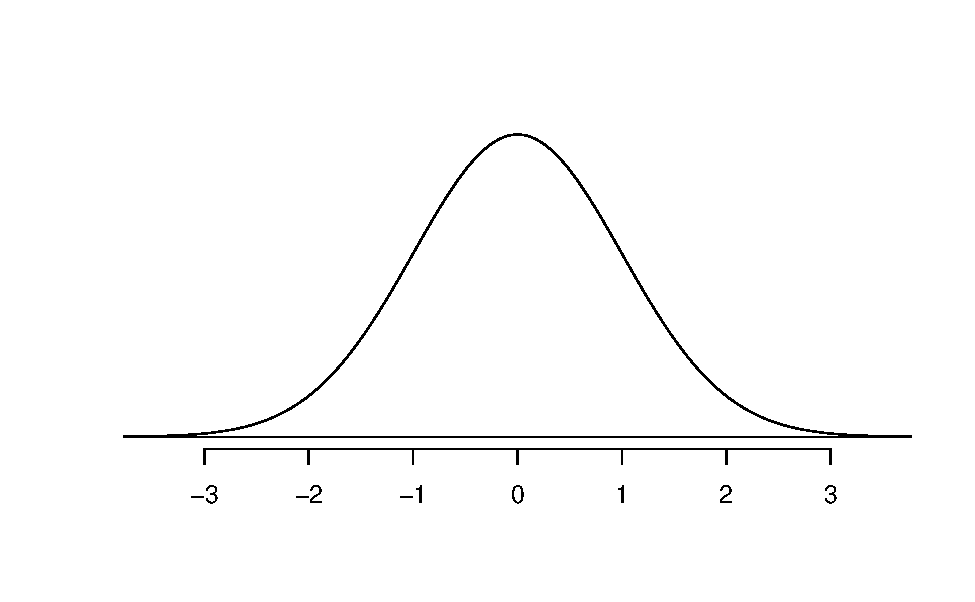
\includegraphics[width=0.6\linewidth]{10-A15-inference-2cat_test-theory_files/figure-latex/simpleNormal-1} 

}

\caption{A standard normal curve.}\label{fig:simpleNormal}
\end{figure}

\begin{enumerate}
\def\labelenumi{\arabic{enumi}.}
\setcounter{enumi}{9}
\tightlist
\item
  Mark the value of the standardized statistic on the standard normal distribution above and shade the area to find the p-value.
\end{enumerate}

\vspace{0.1in}

We will use the \texttt{pnorm()} function in \texttt{R} to find the p-value. Use the provided \texttt{R} script file and enter the value of the standardized statistic found in question 8 at \texttt{xx} in line 1; highlight and run lines 1--3.

\begin{Shaded}
\begin{Highlighting}[]
\FunctionTok{pnorm}\NormalTok{(xx, }\CommentTok{\# Enter value of standardized statistic}
      \AttributeTok{m=}\DecValTok{0}\NormalTok{, }\AttributeTok{s=}\DecValTok{1}\NormalTok{, }\CommentTok{\# Using the standard normal mean = 0, sd = 1}
      \AttributeTok{lower.tail=}\ConstantTok{TRUE}\NormalTok{) }\CommentTok{\# Gives a p{-}value less than the standardized statistic}
\end{Highlighting}
\end{Shaded}

\begin{enumerate}
\def\labelenumi{\arabic{enumi}.}
\setcounter{enumi}{10}
\item
  Report the p-value from the \texttt{R} output.
  \vspace{0.2in}
\item
  Interpret the p-value in context of the study.
\end{enumerate}

\vspace{0.5in}

\begin{enumerate}
\def\labelenumi{\arabic{enumi}.}
\setcounter{enumi}{12}
\tightlist
\item
  Write a conclusion to the research question based on the p-value found.
\end{enumerate}

\vspace{1in}

\newpage

\hypertarget{relative-risk}{%
\subsubsection*{Relative Risk}\label{relative-risk}}
\addcontentsline{toc}{subsubsection}{Relative Risk}

Another summary statistic that can be calculated for two categorical variables is the relative risk. The relative risk is calculated as the ratio of the conditional proportions:

\[\text{relative risk} = \frac{\hat{p}_1}{\hat{p}_2}.\]

\begin{enumerate}
\def\labelenumi{\arabic{enumi}.}
\setcounter{enumi}{13}
\tightlist
\item
  Calculate the relative risk of helping for those who were assigned to the hurry condition compared to those who were not.
\end{enumerate}

\vspace{.8in}

\begin{enumerate}
\def\labelenumi{\arabic{enumi}.}
\setcounter{enumi}{14}
\tightlist
\item
  Interpret the relative risk in context of the problem.
\end{enumerate}

\vspace{1in}

\hypertarget{take-home-messages-15}{%
\subsection{Take-home messages}\label{take-home-messages-15}}

\begin{enumerate}
\def\labelenumi{\arabic{enumi}.}
\item
  When comparing two groups, we are looking at the difference between two parameters. In the null hypothesis, we assume the two parameters are equal, or that there is no difference between the two proportions.
\item
  The standardized statistic when the response variable is categorical is a Z-score and is compared to the standard normal distribution to find the p-value. To find the standardized statistic, we take the value of the statistic minus the null value, divided by the null standard error of the statistic. The standardized statistic measures the number of standard errors the statistic is from the null value.
\item
  Relative risk evaluates the percent increase or percent decrease in the response variable attributed to the explanatory variable. To find the percent increase or percent decrease we calculate the following \(\text{percent change}=(RR - 1)x100\%\). If relative risk is less than 1 there is a percent decrease. If relative risk is greater than 1 there is a percent increase.
\end{enumerate}

\hypertarget{additional-notes-14}{%
\subsection{Additional notes}\label{additional-notes-14}}

Use this space to summarize your thoughts and take additional notes on today's activity and material covered.

\newpage

\hypertarget{week-10b-winter-sports-helmet-use-and-head-injuries-theory-ci}{%
\section{Week 10b: Winter Sports Helmet Use and Head Injuries --- Theory CI}\label{week-10b-winter-sports-helmet-use-and-head-injuries-theory-ci}}

\setstretch{1}

\hypertarget{learning-objectives-16}{%
\subsection{Learning objectives}\label{learning-objectives-16}}

\begin{itemize}
\item
  Assess the conditions to use the normal distribution model for a difference in proportions.
\item
  Create and interpret a theory-based confidence interval for a difference in proportions.
\end{itemize}

\hypertarget{terminology-review-17}{%
\subsection{Terminology review}\label{terminology-review-17}}

In this week's activity, we will use theory-based methods to estimate the difference in two proportions. Some terms covered in this activity are:

\begin{itemize}
\item
  Standard normal distribution
\item
  Independence and success-failure conditions
\end{itemize}

To review these concepts, see Chapter 5 in your textbook.

In this activity we will focus on theory-based methods to calculate a confidence interval. Like with a single proportion, the sampling distribution of a difference in proportions can be mathematically modeled using the normal distribution if certain conditions are met.

Conditions for the sampling distribution of \(\hat{p}_1-\hat{p}_2\) to follow an approximate normal distribution:

\begin{itemize}
\item
  \textbf{Independence}: The data are independent within and between the two groups. (\emph{Remember}: This also must be true to use simulation methods!)
\item
  \textbf{Success-failure condition}: The success-failure condition holds for each group. Since we are not assuming a null hypothesis, we do not use the pooled sample proportion to check this condition as we did in Activity 8. Instead, we use the individual sample proportions \(\hat{p}_1\) and \(\hat{p}_2\). Equivalently, we check that all cells in the table have at least 10 observations.
\end{itemize}

\begin{enumerate}
\def\labelenumi{\arabic{enumi}.}
\tightlist
\item
  Explain why a theory-based confidence interval for the data set in Activities 9a and 9b would not be similar to the bootstrap interval created.
\end{enumerate}

\vspace{1in}

For this activity we will again use the Helmet Use and Head Injury data set. In Activity 10a we saw that there was evidence that helmet use is assoicated with a reduced risk of head injury. Today we will estimate the difference in proportion of head injuries for those who wore helmets and those who did not.

In ``Helmet Use and Risk of Head Injuries in Alpine Skiers and Snowboarders'' by Sullheim et. al., in the \emph{Journal of the American Medical Association}, Vol. 295, No.~8 (2006), we can see the summary results from a random sample of 3562 skiers and snowboarders involved in accidents in the two-way table below.

\begin{longtable}[]{@{}cccc@{}}
\toprule
& Helmet Use & No Helmet Use & Total \\
\midrule
\endhead
Head Injury & 96 & 480 & 576 \\
No Head Injury & 656 & 2330 & 2986 \\
Total & 752 & 2810 & 3562 \\
\bottomrule
\end{longtable}

\begin{enumerate}
\def\labelenumi{\arabic{enumi}.}
\setcounter{enumi}{1}
\tightlist
\item
  In the last activity we verified that the independence condtion was met. Is the success-failure condition to find the theory-based confidence interval met for each group? Explain your answer.
\end{enumerate}

\vspace{1in}

\begin{enumerate}
\def\labelenumi{\arabic{enumi}.}
\setcounter{enumi}{2}
\tightlist
\item
  Write the parameter of interest for this study in context of the problem.
\end{enumerate}

\vspace{0.8in}

To find a confidence interval for the difference in proportions we will add and subtract the margin of error from the point estimate to find the two endpoints.

\[\hat{p}_1-\hat{p}_2\pm z^*SE(\hat{p}_1-\hat{p}_2), \hspace{.2cm} \text{where}\]
\[SE(\hat{p}_1-\hat{p}_2) = \sqrt{\frac{\hat{p}_1 (1-\hat{p}_1)}{n_1}+\frac{\hat{p}_2 (1-\hat{p}_2)}{n_2}}\]

Note that the formula changes when calculating the variability around the statistic in order to calculate a confidence interval from the formula used in Activity 10a! Here, we use the sample proportions for each group to calculate the standard error for the difference in proportions since we are not assuming that the true difference is zero.

\begin{enumerate}
\def\labelenumi{\arabic{enumi}.}
\setcounter{enumi}{3}
\tightlist
\item
  Calculate the standard error for a difference in proportions to create a 90\% confidence interval.
\end{enumerate}

\vspace{1in}

\begin{enumerate}
\def\labelenumi{\arabic{enumi}.}
\setcounter{enumi}{4}
\tightlist
\item
  Interpret the value calculated in question 4 in context of the problem.
\end{enumerate}

\vspace{1in}
\newpage

Recall that the \(z^*\) multiplier is the percentile of a standard normal distribution that corresponds to our confidence level. If our confidence level is 90\%, we find the Z values that encompass the middle 90\% of the standard normal distribution. If 90\% of the standard normal distribution should be in the middle, that leaves 10\% in the tails, or 5\% in each tail. The \texttt{qnorm()} function in \texttt{R} will tell us the \(z^*\) value for the desired percentile (in this case, 90\% + 5\% = 95\% percentile).

\begin{Shaded}
\begin{Highlighting}[]
\FunctionTok{qnorm}\NormalTok{(}\FloatTok{0.95}\NormalTok{) }\CommentTok{\# Multiplier for 90\% confidence interval}
\end{Highlighting}
\end{Shaded}

\begin{verbatim}
#> [1] 1.644854
\end{verbatim}

\begin{enumerate}
\def\labelenumi{\arabic{enumi}.}
\setcounter{enumi}{5}
\tightlist
\item
  Sketch a graph of the standard normal distribution and use the graph to explain how the \texttt{R} code above is used to find the \(z^*\) multiplier.
\end{enumerate}

\vspace{1.5in}

\begin{enumerate}
\def\labelenumi{\arabic{enumi}.}
\setcounter{enumi}{6}
\tightlist
\item
  Using the multiplier of \(z^*\) = 1.645 and the standard error found in question 4, calculate the margin of error for a 90\% confidence interval.
\end{enumerate}

\vspace{0.5in}

\begin{enumerate}
\def\labelenumi{\arabic{enumi}.}
\setcounter{enumi}{7}
\tightlist
\item
  Calculate the 90\% confidence interval for the parameter of interest.
\end{enumerate}

\vspace{1in}

\begin{enumerate}
\def\labelenumi{\arabic{enumi}.}
\setcounter{enumi}{8}
\tightlist
\item
  Interpret the confidence interval found in question 8 in context of the problem.
\end{enumerate}

\vspace{1in}

\begin{enumerate}
\def\labelenumi{\arabic{enumi}.}
\setcounter{enumi}{9}
\tightlist
\item
  Interpret the level of confidence in context of the problem. What does it mean to be 90\% confident in the confidence interval?
\end{enumerate}

\vspace{0.8in}

\begin{enumerate}
\def\labelenumi{\arabic{enumi}.}
\setcounter{enumi}{10}
\tightlist
\item
  What decision would you make based on your confidence interval? Explain your answer.
  \vspace{0.5in}
\end{enumerate}

\hypertarget{effect-of-sample-size-2}{%
\subsection{Effect of sample size}\label{effect-of-sample-size-2}}

Suppose in another sample of skiers and snowboards involved in accidents we saw these results:

\begin{longtable}[]{@{}cccc@{}}
\toprule
& Helmet Use & No Helmet Use & Total \\
\midrule
\endhead
Head Injury & 135 & 674 & 809 \\
No Head Injury & 921 & 3270 & 4191 \\
Total & 1056 & 3944 & 5000 \\
\bottomrule
\end{longtable}

\begin{enumerate}
\def\labelenumi{\arabic{enumi}.}
\setcounter{enumi}{11}
\tightlist
\item
  Calculate the margin of error for a 90\% confidence interval using a multiplier of \(z^*\) = 1.645 for this new sample. Is the margin of error larger or smaller than the margin of error for the original study?
\end{enumerate}

\vspace{.8in}

\begin{enumerate}
\def\labelenumi{\arabic{enumi}.}
\setcounter{enumi}{12}
\tightlist
\item
  Calculate the 90\% confidence interval for this new study using the margin of error from question 12.
\end{enumerate}

\vspace{.8in}

\begin{enumerate}
\def\labelenumi{\arabic{enumi}.}
\setcounter{enumi}{13}
\tightlist
\item
  Is the confidence interval calculated in question 13 with the smaller sample size wider or smaller than the confidence interval in question 8? Why?
\end{enumerate}

\vspace{.8in}

\hypertarget{take-home-messages-16}{%
\subsection{Take-home messages}\label{take-home-messages-16}}

\begin{enumerate}
\def\labelenumi{\arabic{enumi}.}
\item
  Simulation-based methods and theory-based methods should give the same results for a study \emph{if the validity conditions are met}. For both methods, observational units need to be independent. To use theory-based methods, additionally, the success-failure condition must be met. Check the validity conditions for each type of test to determine if theory-based methods can be used.
\item
  When calculating the standard error for the difference in sample proportions when doing a hypothesis test, we use the pooled proportion of successes, the best estimate for calculating the variability \emph{under the assumption the null hypothesis is true}. For a confidence interval, we are not assuming a null hypothesis, so we use the values of the two conditional proportions to calculate the standard error. Make note of the difference in these two formulas.
\item
  Increasing sample size will result in less sample-to-sample variability in statistics, which will result in a smaller standard error, and thus a narrower confidence interval.
\end{enumerate}

\hypertarget{additional-notes-15}{%
\subsection{Additional notes}\label{additional-notes-15}}

Use this space to summarize your thoughts and take additional notes on today's activity and material covered.

\newpage

\hypertarget{week-10---lab-8-diabetes}{%
\section{Week 10 - Lab 8: Diabetes}\label{week-10---lab-8-diabetes}}

\setstretch{1}

\hypertarget{learning-objectives-17}{%
\subsection{Learning objectives}\label{learning-objectives-17}}

\begin{itemize}
\item
  Given a research question involving two categorical variables, construct the null and alternative hypotheses
  in words and using appropriate statistical symbols.
\item
  Assess the conditions to use the normal distribution model for a difference in proportions.
\item
  Calculate the Z test statistic for a difference in proportions.
\item
  Find, interpret, and evaluate the p-value for a theory-based hypothesis test for a difference in proportions.
\item
  Create and interpret a theory-based confidence interval for a difference in proportions.
\end{itemize}

\hypertarget{glycemic-control-in-diabetic-adolescents}{%
\subsection{Glycemic Control in Diabetic Adolescents}\label{glycemic-control-in-diabetic-adolescents}}

Researchers compared the efficacy of two treatment regimens to achieve durable glycemic control in children and adolescents with recent-onset type 2 diabetes. A convenience sample of patients 10 to 17 years of age with recent-onset type 2 diabetes were randomly assigned to either a medication (rosiglitazone) or a lifestyle-intervention program focusing on weight loss through eating and activity. Researchers measured whether the patient still needs insulin (failure) or had glycemic control (success). Of the 233 children who received the Rosiglitazone treatment,143 had glycemic control, while of the 234 who went through the lifestyle-intervention program, 125 had glycemic control. Is there evidence that there is difference in proportion of patients that achieve durable glycemic control between the two treatments? Use Rosiglitazone -- Lifestyle as the order of subtraction.

Upload and open the \texttt{R} script file for Week 10 lab. Upload and import the csv file, \texttt{diabetes}. Enter the name of the data set (see the environment tab) for \texttt{datasetname} in the R script file in line 4. Highlight and run lines 1--5 to get the counts for each combination of categories.

\begin{Shaded}
\begin{Highlighting}[]
\NormalTok{datasetname }\OtherTok{{-}\textgreater{}}\NormalTok{ diabetes}
\NormalTok{diabetes }\SpecialCharTok{\%\textgreater{}\%} \FunctionTok{group\_by}\NormalTok{(treatment) }\SpecialCharTok{\%\textgreater{}\%} \FunctionTok{count}\NormalTok{(outcome)}
\end{Highlighting}
\end{Shaded}

\begin{enumerate}
\def\labelenumi{\arabic{enumi}.}
\tightlist
\item
  Complete the following two-way table using the data above.
\end{enumerate}

\begin{longtable}[]{@{}llll@{}}
\toprule
& Rosiglitazone & Lifestyle & Total \\
\midrule
\endhead
Glycemic Control & & & \\
Insulin Required & & & \\
Total & & & \\
\bottomrule
\end{longtable}

\begin{enumerate}
\def\labelenumi{\arabic{enumi}.}
\setcounter{enumi}{1}
\tightlist
\item
  Is the independence condition met for this study? Explain your answer.
\end{enumerate}

\vspace{0.8in}

\begin{enumerate}
\def\labelenumi{\arabic{enumi}.}
\setcounter{enumi}{2}
\item
  Is the success-failure condition to use theory-based methods for a hypothesis test met for each group. Explain your answer.
  \vspace{1in}
\item
  Is the success-failure condition to find the theory-based confidence interval met for each group? Explain your answer.
\end{enumerate}

\vspace{1in}

\begin{enumerate}
\def\labelenumi{\arabic{enumi}.}
\setcounter{enumi}{4}
\tightlist
\item
  Write the parameter of interest for this study in context of the problem.
\end{enumerate}

\vspace{0.8in}

To find a confidence interval for the difference in proportions we will add and subtract the margin of error from the point estimate to find the two endpoints.

\[\hat{p}_1-\hat{p}_2\pm z^*SE(\hat{p}_1-\hat{p}_2), \hspace{.2cm} \text{where}\]
\[SE(\hat{p}_1-\hat{p}_2) = \sqrt{\frac{\hat{p}_1 (1-\hat{p}_1)}{n_1}+\frac{\hat{p}_2 (1-\hat{p}_2)}{n_2}}\]

Note that the formula changes when calculating the variability around the statistic in order to calculate a confidence interval from the formula used in Activity 19! Here, we use the sample proportions for each group to calculate the standard error for the difference in proportions since we are not assuming that the true difference is zero.

\begin{enumerate}
\def\labelenumi{\arabic{enumi}.}
\setcounter{enumi}{5}
\tightlist
\item
  Calculate the standard error for a difference in proportions to create a 95\% confidence interval.
\end{enumerate}

\vspace{1in}

\begin{enumerate}
\def\labelenumi{\arabic{enumi}.}
\setcounter{enumi}{6}
\tightlist
\item
  Interpret the value calculated in question 5 in context of the problem.
\end{enumerate}

\vspace{1in}

\newpage

The \(z^*\) multiplier is the percentile of a standard normal distribution that corresponds to our confidence level. If our confidence level is 90\%, we find the Z values that encompass the middle 90\% of the standard normal distribution. If 90\% of the standard normal distribution should be in the middle, that leaves 10\% in the tails, or 5\% in each tail. The \texttt{qnorm()} function in \texttt{R} will tell us the \(z^*\) value for the desired percentile (in this case, 90\% + 5\% = 95\% percentile).

\begin{Shaded}
\begin{Highlighting}[]
\FunctionTok{qnorm}\NormalTok{(}\FloatTok{0.95}\NormalTok{) }\CommentTok{\# Multiplier for 90\% confidence interval}
\end{Highlighting}
\end{Shaded}

\begin{verbatim}
#> [1] 1.644854
\end{verbatim}

\begin{enumerate}
\def\labelenumi{\arabic{enumi}.}
\setcounter{enumi}{7}
\tightlist
\item
  Sketch a graph of the standard normal distribution and use the graph to explain how the \texttt{R} code above is used to find the \(z^*\) multiplier.
\end{enumerate}

\vspace{1.5in}

\begin{enumerate}
\def\labelenumi{\arabic{enumi}.}
\setcounter{enumi}{8}
\tightlist
\item
  Using the multiplier of \(z^*\) = 1.645 and the standard error found in question 5, calculate the margin of error for a 90\% confidence interval.
\end{enumerate}

\vspace{0.5in}

\begin{enumerate}
\def\labelenumi{\arabic{enumi}.}
\setcounter{enumi}{9}
\tightlist
\item
  Calculate the 90\% confidence interval for the difference in true proportion of .
\end{enumerate}

\vspace{1in}

\begin{enumerate}
\def\labelenumi{\arabic{enumi}.}
\setcounter{enumi}{10}
\tightlist
\item
  Interpret the confidence interval found in question 10 in context of the problem.
\end{enumerate}

\vspace{1in}

\hypertarget{exam-2-review}{%
\chapter{Exam 2 Review}\label{exam-2-review}}

Use the provided data set from the Islands (ExamReviewData.csv) and the Exam 2 Review \texttt{R} script file to answer the following questions. Each adult (\textgreater21) islander was selected at random from all the adult islanders.

\begin{longtable}[]{@{}
  >{\raggedright\arraybackslash}p{(\columnwidth - 2\tabcolsep) * \real{0.24}}
  >{\raggedright\arraybackslash}p{(\columnwidth - 2\tabcolsep) * \real{0.76}}@{}}
\toprule
\textbf{Variable} & \textbf{Description} \\
\midrule
\endhead
\texttt{Island} & Name of Island that the Islander resides on \\
\texttt{City} & Name of City in which the Islander resides \\
\texttt{Population} & Population of the City \\
\texttt{Name} & Name of Islander \\
\texttt{Consent} & Whether the Islander consented to be in the study \\
\texttt{Gender} & Gender of Islander (M = male, F = Female) \\
\texttt{Age} & Age of Islander \\
\texttt{Married} & Marital status of Islander \\
\texttt{Smoking\_Status} & Whether the Islander is a current smoker \\
\texttt{Children} & Whether the Islander has children \\
\texttt{weight\_kg} & Weight measured in kg \\
\texttt{height\_cm} & Height measured in cm \\
\texttt{respitory\_rate} & Breaths per minute \\
\texttt{Type\_of\_Music} & Music type (Classical or Heavy Medal) Islander was randomly assigned to listen to \\
\texttt{Before\_PuzzleCube} & Time to complete puzzle cube (minutes) before listening to assigned music \\
\texttt{After\_PuzzleCube} & Time to complete puzzle cube (minutes) after listening to assigned music \\
\texttt{Diff\_PuzzleCube} & Difference in time to complete puzzle cube (minutes) for Before - After listening to assigned music \\
\texttt{Education\_Level} & Highest level of education completed (note: missing data depicted by missing) \\
\texttt{Balance\_Test} & Time balanced measured in seconds with eyes closed \\
\texttt{Blood\_Glucose\_before} & Level of blood glucose (mg/dL) before consuming assigned drink \\
\texttt{Heart\_Rate\_before} & Heart rate (bpm) before consuming assigned drink \\
\texttt{Type\_of\_Drink} & Type of drink (EnergyDrink or Cola) Islander was randomly assigned to drink \\
\texttt{Heart\_Rate\_after} & Heart rate (bpm) after consuming assigned drink \\
\texttt{Blood\_Glucose\_after} & Level of blood glucose (mg/dL) after consuming assigned drink \\
\texttt{Diff\_Heart\_Rate} & Difference in heart rate (bpm) for Before - After consuming assigned drink \\
\texttt{Diff\_Blood\_Glucose} & Difference in blood glucose (mg/dL) for Before - After consuming assigned drink \\
\bottomrule
\end{longtable}

\begin{enumerate}
\def\labelenumi{\arabic{enumi}.}
\tightlist
\item
  Write a research question involving a single categorical variable that can be answered using the data set.
\end{enumerate}

\vspace{0.8in}

\begin{enumerate}
\def\labelenumi{\arabic{enumi}.}
\setcounter{enumi}{1}
\tightlist
\item
  Use the provided Exam 2 Review \texttt{R} script file and analyze this research question.
\end{enumerate}

\rgi Parameter of Interest:

\vspace{0.3in}

\rgi Null Hypothesis:

\rgi \rgi Notation:

\vspace{0.3in}

\rgi \rgi Words:

\vspace{0.5in}

\rgi Alternative Hypothesis:

\rgi \rgi Notation:

\vspace{0.3in}

\rgi \rgi Words:

\vspace{0.5in}

\rgi Statistic:

\vspace{0.3in}

\rgi Conditions:

\rgi \rgi Independence:

\vspace{0.8in}

\rgi \rgi Success-Failure:

\vspace{0.8in}

\rgi Simulation P-value:

\vspace{0.3in}

\rgi \rgi Interpretation:

\vspace{0.8in}

\rgi \rgi Conclusion:

\vspace{0.8in}

\rgi \rgi Decision:

\vspace{0.3in}

\rgi Simulation Confidence Interval:

\vspace{0.3in}

\rgi \rgi Interpretation:

\vspace{0.8in}

\rgi Standardized Statistic:

\vspace{0.3in}

\rgi \rgi Interpretation:

\vspace{0.8in}

\rgi Theory-based p-value:

\vspace{0.3in}

\rgi Theory-based Confidence Interval:

\vspace{0.3in}

\rgi Does the theory-based p-value and CI match those found using simulation methods?

\vspace{0.8in}

\rgi To what group can the results be generalized?

\vspace{0.8in}

\begin{enumerate}
\def\labelenumi{\arabic{enumi}.}
\setcounter{enumi}{2}
\tightlist
\item
  Write a research question involving two categorical variables that can be answered using the data set.
\end{enumerate}

\vspace{0.8in}

\begin{enumerate}
\def\labelenumi{\arabic{enumi}.}
\setcounter{enumi}{3}
\item
  Use the provided Exam 2 Review \texttt{R} script file and analyze this research question.

  \rgi Parameter of Interest:
\end{enumerate}

\vspace{0.3in}

\rgi Null Hypothesis:

\rgi \rgi Notation:

\vspace{0.3in}

\rgi \rgi Words:

\vspace{0.5in}

\rgi Alternative Hypothesis:

\rgi \rgi Notation:

\vspace{0.3in}

\rgi \rgi Words:

\vspace{0.5in}

\rgi Statistic:

\vspace{0.3in}

\rgi Conditions:

\rgi \rgi Independence:

\vspace{0.8in}

\rgi \rgi Success-Failure:

\vspace{0.8in}

\rgi Simulation P-value:

\vspace{0.3in}

\rgi \rgi Interpretation:

\vspace{0.8in}

\rgi \rgi Conclusion:

\vspace{0.8in}

\rgi \rgi Decision:

\vspace{0.3in}

\rgi Simulation Confidence Interval:

\vspace{0.3in}

\rgi \rgi Interpretation:

\vspace{0.8in}

\rgi Standardized Statistic:

\vspace{0.3in}

\rgi \rgi Interpretation:

\vspace{0.8in}

\rgi Theory-based p-value:

\vspace{0.3in}

\rgi Theory-based Confidence Interval:

\vspace{0.3in}

\rgi Does the theory-based p-value and CI match those found using simulation methods?

\vspace{0.8in}

\rgi What is the scope of inference for this study?

\vspace{0.8in}

\newpage

\hypertarget{inference-for-a-quantitative-response-with-paired-samples}{%
\chapter{Inference for a Quantitative Response with Paired Samples}\label{inference-for-a-quantitative-response-with-paired-samples}}

\hypertarget{reading-guide-inference-for-a-single-mean-or-paired-mean-difference}{%
\section{Reading Guide: Inference for a Single Mean or Paired Mean Difference}\label{reading-guide-inference-for-a-single-mean-or-paired-mean-difference}}

\hypertarget{section-6.1-inference-for-one-mean}{%
\subsection*{Section 6.1 (Inference for one mean)}\label{section-6.1-inference-for-one-mean}}
\addcontentsline{toc}{subsection}{Section 6.1 (Inference for one mean)}

\textbf{Videos}

\begin{itemize}
\tightlist
\item
  6.1
\end{itemize}

\setstretch{1.25}

\hypertarget{reminders-from-previous-sections-5}{%
\subsubsection*{Reminders from previous sections}\label{reminders-from-previous-sections-5}}
\addcontentsline{toc}{subsubsection}{Reminders from previous sections}

\(n\) = sample size

\(\overline{x}\) = sample mean

\(s\) = sample standard deviation

\(\mu\) = population mean

\(\sigma\) = population standard deviation

General steps of a hypothesis test:

\begin{enumerate}
\def\labelenumi{\arabic{enumi}.}
\item
  Frame the research question in terms of hypotheses.
\item
  Collect and summarize data using a test statistic.
\item
  Assume the null hypothesis is true, and simulate or mathematically model a null distribution for the test statistic.
\item
  Compare the observed test statistic to the null distribution to calculate a p-value.
\item
  Make a conclusion based on the p-value and write the conclusion in context.
\end{enumerate}

Parameter: a value summarizing a variable(s) for a population.

Statistic: a value summarizing a variable(s) for a sample.

Sampling distribution: plot of statistics from 1000s of samples of the same size taken from the same population.

Standard deviation of a statistic: the variability of statistics from 1000s of samples; how far, on average, each statistic is from the true value of the parameter.

Standard error of a statistic: estimated standard deviation of a statistic.

Hypothesis test: a process to determine how strong the evidence of an effect is. Also called a `significance test.'

Simulation-based method: Simulate lots of samples of size \(n\) under assumption of the null hypothesis, then find the proportion of the simulations that are at least as extreme as the observed sample statistic.

Theory-based method: Develop a mathematical model for the sampling distribution of the statistic under the null hypothesis and use the model to calculate the probability of the observed sample statistic (or one more extreme) occurring.

Null hypothesis (\(H_0\)): the skeptical perspective; no difference; no change; no effect; random chance; what the researcher hopes to prove is \textbf{wrong}.

Alternative hypothesis (\(H_A\)): the new perspective; a difference/increase/decrease; an effect; not random chance; what the researcher hopes to prove is \textbf{correct}.

Null value: the value of the parameter when we assume the null hypothesis is true (labeled as \(parameter_0\)).

Null distribution: the simulated or modeled distribution of statistics (sampling distribution) we would expect to occur if the null hypothesis is true.

P-value: probability of seeing the observed sample data, or something more extreme, assuming the null hypothesis is true.

\(\implies\) Lower the p-value the stronger the evidence AGAINST the null hypothesis and FOR the alternative hypothesis.

Decision: a determination of whether to reject or fail to reject a null hypothesis based on a p-value and a pre-set level of significance.

\begin{itemize}
\item
  If p-value \(\leq \alpha\), then reject \(H_0\).
\item
  If p-value \(> \alpha\), then fail to reject \(H_0\).
\end{itemize}

Significance level (\(\alpha\)): a threshold used to determine if a p-value provides enough evidence to reject the null hypothesis or not.

\rgi Common levels of \(\alpha\) include 0.01, 0.05, and 0.10.

Statistically significant: results are considered statistically significant if the p-value is below the significance level.

Confidence interval: a process to determine how large an effect is; a range of plausible values for the parameter. Also called `estimation.'

Margin of error: the value that is added to and subtracted from the sample statistic to create a confidence interval; half the width of a confidence interval.

Bootstrapping: the process of drawing with replacement \(n\) times from the original sample.

Bootstrapped resample: a random sample of size \(n\) from the original sample, selected with replacement.

Bootstrapped statistic: the statistic recorded from the bootstrapped resample.

Confidence level: how confident we are that the confidence interval will capture the parameter.

Bootstrap \(X\)\% confidence interval: (\((\frac{(1-X)}{2})^{th}\) percentile, \((X+(\frac{(1-X)}{2})^{th}\) percentile) of a bootstrap distribution.

Central Limit Theorem: For large sample sizes, the sampling distribution of a sample mean (or proportion) will be approximately normal (bell-shaped and symmetric).

\hypertarget{vocabulary-17}{%
\subsubsection*{Vocabulary}\label{vocabulary-17}}
\addcontentsline{toc}{subsubsection}{Vocabulary}

\(t\)-distribution:
\rgs 

\begin{itemize}
\item
  The variability in the \(t\)-distribution depends on the sample size (used to calculate degrees of freedom --- df for short).
\item
  The larger df, the closer the \(t\) distribution is to the standard normal distribution.
\end{itemize}

Degrees of freedom (df):
\rgs 

T-score:
\rgs 

\hypertarget{notes-22}{%
\subsubsection*{Notes}\label{notes-22}}
\addcontentsline{toc}{subsubsection}{Notes}

To create a bootstrap distribution test, how many cards will you need and how will the cards be labeled?
\rgs 

What do you do with the cards after labeling them?
\rgs 

After resampling, what value will be plotted on the bootstrap distribution?
\rgs 

True or false: Bootstrapping can only be used if the sample size is small.
\rgs 

Why do we use a \(t\)-distribution rather than the normal distribution when analyzing quantitative data?
\rgs 

How do we calculate degrees of freedom for the \(t\)-distribution?
\rgs 

Conditions to use the CLT for means:

\rgi Independence:
\rgs 

\rgi \rgi Checked by:
\rgs 

\rgi Normality:
\rgs 

\rgi \rgi Checked by:
\rgs 

\hypertarget{formulas-5}{%
\subsubsection*{Formulas}\label{formulas-5}}
\addcontentsline{toc}{subsubsection}{Formulas}

\(SE(\overline{x})=\)
\rgs 

\(T=\)
\rgs 

Confidence interval for a mean:
\rgs 

\hypertarget{notation-2}{%
\subsubsection*{Notation}\label{notation-2}}
\addcontentsline{toc}{subsubsection}{Notation}

\(\mu_0\) represents
\rgs 

\hypertarget{example-edinburgh-rentals}{%
\subsubsection*{Example: Edinburgh rentals}\label{example-edinburgh-rentals}}
\addcontentsline{toc}{subsubsection}{Example: Edinburgh rentals}

\begin{enumerate}
\def\labelenumi{\arabic{enumi}.}
\item
  What are the observational units?
  \rgs 
\item
  What are the sample statistics presented in this example? What notation would be used to represent each value?
  \rgs 
\item
  What is the parameter representing in the context of this problem? What notation would be used to represent this parameter?
  \rgs 
  \rgs 
\item
  How could we use cards to simulate \textbf{one} bootstrap resample \emph{which does not assume the null hypothesis is true}? How many cards? What is written on the cards? What would we do with the cards? What would you record once you have a simulated sample?
  \rgs 
  \rgs 
  \rgs 
\item
  After 1000 resamples are generated, where is the resulting bootstrap distribution centered? Why does that make sense?
  \rgs 
  \rgs 
\item
  Based on Figure 6.3, give the confidence interval for each of the following confidence levels.
\end{enumerate}

\rgi 90\% confidence interval =
\rgs 

\rgi 95\% confidence interval =
\rgs 

\rgi 99\% confidence interval =
\rgs 

\begin{enumerate}
\def\labelenumi{\arabic{enumi}.}
\setcounter{enumi}{6}
\item
  Interpret your 99\% confidence interval in the context of the problem.
  \rgs 
  \rgs 
\item
  Use Figure 6.4 to determine a 90\% confidence interval for the true standard deviation for three bedroom flats in Edinburgh.
  \rgs 
\end{enumerate}

\hypertarget{example-mercury-content-of-dolphin-muscle}{%
\subsubsection*{Example: Mercury content of dolphin muscle}\label{example-mercury-content-of-dolphin-muscle}}
\addcontentsline{toc}{subsubsection}{Example: Mercury content of dolphin muscle}

\begin{enumerate}
\def\labelenumi{\arabic{enumi}.}
\item
  What is the research question?
  \rgs 
\item
  What are the observational units?
  \rgs 
\item
  Can the results of this study be generalized to a larger population? Why or why not?
  \rgs 
\item
  What are the sample statistics presented in this example? What notation would be used to represent each value?
  \rgs 
\item
  What is the parameter representing in the context of this problem? What notation would be used to represent this parameter?
  \rgs 
  \rgs 
\item
  Are the independence and normality conditions satisfied?
  \rgs 
  \rgs 
\item
  Calculate the standard error of the sample mean.
  \rgs 
  \rgs
\item
  What distribution should be referenced to find the multiplier for a 95\% confidence interval?
  \rgs 
\item
  Using \(t^\star=2.10\), calculate a 95\% confidence interval for \(\mu\).
  \rgs 
  \rgs
\item
  Interpret the interval calculated in the context of the problem.
  \rgs 
  \rgs 
\end{enumerate}

\hypertarget{example-cherry-blossom-race}{%
\subsubsection*{Example: Cherry Blossom Race}\label{example-cherry-blossom-race}}
\addcontentsline{toc}{subsubsection}{Example: Cherry Blossom Race}

\begin{enumerate}
\def\labelenumi{\arabic{enumi}.}
\item
  What is the research question?
  \rgs
\item
  What are the observational units?
  \rgs
\item
  Can the results of this study be generalized to a larger population? Why or why not?
  \rgs
\item
  What are the sample statistics presented in this example? What notation would be used to represent each value?
  \rgs
\item
  What is the parameter representing in the context of this problem? What notation would be used to represent this parameter?
  \rgs
  \rgs
\item
  Are the independence and normality conditions satisfied?
  \rgs
  \rgs
\item
  Write the null and the alternative hypotheses in words.
  \rgs
  \rgs
\item
  Write the null and the alternative hypotheses in notation.
  \rgs
\item
  Calculate the standard error of the sample mean.
  \rgs
  \rgs
\item
  Calculate the T-score (the standardized statistic for the sample mean).
  \rgs
  \rgs
\item
  What distribution should the T-score be compared to in order to calculate a p-value?
  \rgs
\item
  What was the p-value of the test?
  \rgs
\item
  Interpret the p-value in the context of the problem.
  \rgs
  \rgs
\item
  At the 5\% significance level, what decision would you make? What type of error might that be?
  \rgs
\item
  What conclusion should the researcher make?
  \rgs
  \rgs
\item
  Are the results in this example statistically significant? Justify your answer.
  \rgs
\end{enumerate}

\hypertarget{section-6.2-inference-for-paired-mean-difference}{%
\subsection*{Section 6.2 (Inference for paired mean difference)}\label{section-6.2-inference-for-paired-mean-difference}}
\addcontentsline{toc}{subsection}{Section 6.2 (Inference for paired mean difference)}

\setstretch{1}

\textbf{Videos}

\begin{itemize}
\tightlist
\item
  6.2
\end{itemize}

\setstretch{1.25}

\hypertarget{vocabulary-18}{%
\subsubsection*{Vocabulary}\label{vocabulary-18}}
\addcontentsline{toc}{subsubsection}{Vocabulary}

Paired data:
\rgs

\rgi Paired with repeated measures:
\rgs

\rgi Paired with matching:
\rgs

\hypertarget{notes-23}{%
\subsubsection*{Notes}\label{notes-23}}
\addcontentsline{toc}{subsubsection}{Notes}

For each of the following scenarios, determine if the two sets of observations are paired or independent.

\begin{enumerate}
\def\labelenumi{\arabic{enumi}.}
\item
  To test whether the IQ is related to genetics, researchers measured the IQ of two biological parents and the IQ of their first-born child. The average parent IQ was compared to the IQ of the first born child.
  \rgs
\item
  Hoping to see how exercise is related to heart rates, researchers asked a group of 30 volunteers to do either bicycle kicks or jumping jacks for 30 seconds. Volunteer's heart rate was measured at the end of 30 seconds, then the volunteers sat for a 5 minute rest period. At the end of the rest period, the volunteer performed the other activity and their heart rate was measured again. Which activity was done first was randomly assigned.
  \rgs
\item
  Researchers hoping to look into the effectiveness of blended learning gathered two random samples of 50 8th graders (one at Belgrade Middle School which has 5 full-day instruction currently, the other from Chief Joseph Middle School which utilizes a 2-day on, 3-day off blended learning structure). All 8th graders were given the same lessons and same homework, then asked to take the same end-of-unit test.
  \rgs
\end{enumerate}

Conditions to use the CLT for paired mean difference:

\rgi Independence:
\rgs

\rgi \rgi Checked by:
\rgs 

\rgi Normality:
\rgs

\rgi \rgi Checked by:
\rgs

\hypertarget{formulas-6}{%
\subsubsection*{Formulas}\label{formulas-6}}
\addcontentsline{toc}{subsubsection}{Formulas}

\(SE(\overline{x_d})=\)
\rgs

\(T=\)
\rgs

Confidence interval for a paired mean difference:
\rgs

\hypertarget{notation-3}{%
\subsubsection*{Notation}\label{notation-3}}
\addcontentsline{toc}{subsubsection}{Notation}

\(\overline{x_d}=\)
\rgs

\(s_d=\)
\rgs

\(\mu_d=\)
\rgs

\(\sigma_d=\)
\rgs

\hypertarget{example-tires}{%
\subsubsection*{Example: Tires}\label{example-tires}}
\addcontentsline{toc}{subsubsection}{Example: Tires}

\begin{enumerate}
\def\labelenumi{\arabic{enumi}.}
\item
  What are the observational units?
  \rgs
\item
  Why should we treat these data as paired rather than two independent samples?
  \rgs
\item
  What are the sample statistics presented in this example? What notation would be used to represent each value?
  \rgs
\item
  What is the parameter representing in the context of this problem? What notation would be used to represent this parameter?
  \rgs
  \rgs
\item
  Write the null and alternative hypotheses in appropriate notation.
  \rgs
\item
  How could we use cards to simulate \textbf{one} bootstrap resample \emph{which assumes the null hypothesis is true}? How many cards? What is written on the cards? What would we do with the cards? What would you record once you have a simulated sample?
  \rgs
  \rgs
  \rgs
\item
  After 1000 resamples are generated, where is the resulting null distribution centered? Why does that make sense?
  \rgs
\item
  What was the p-value of the test? Interpret this p-value in the context of the problem.
  \rgs
  \rgs
\item
  Write a conclusion in the context of the problem.
  \rgs
\end{enumerate}

\hypertarget{example-college-textbook-prices}{%
\subsubsection*{Example: College textbook prices}\label{example-college-textbook-prices}}
\addcontentsline{toc}{subsubsection}{Example: College textbook prices}

\begin{enumerate}
\def\labelenumi{\arabic{enumi}.}
\item
  What is the research question?
  \rgs
\item
  What are the observational units?
  \rgs
\item
  Why should we treat these data as paired rather than two independent samples?
  \rgs
\item
  What are the sample statistics presented in this example? What notation would be used to represent each value?
  \rgs
\item
  What is the parameter representing in the context of this problem? What notation would be used to represent this parameter?
  \rgs
  \rgs
\item
  How could we use cards to simulate \textbf{one} bootstrap resample \emph{which does not assume the null hypothesis is true}? How many cards? What is written on the cards? What would we do with the cards? What would you record once you have a simulated sample?
  \rgs
  \rgs
  \rgs
\item
  After 1000 resamples are generated, where is the resulting bootstrap distribution centered? Why does that make sense?
  \rgs
  \rgs
\item
  Give the 95\% confidence interval for \(\mu_d\).
  \rgs
\item
  Interpret your 95\% confidence interval in the context of the problem.
  \rgs
  \rgs
\item
  Are the independence and normality conditions satisfied?
  \rgs
  \rgs
\item
  Write the null and the alternative hypotheses in words.
  \rgs
  \rgs
\item
  Calculate the standard error of the sample mean difference.
  \rgs
  \rgs
\item
  Calculate the T-score (the standardized statistic for the sample mean difference).
  \rgs
  \rgs
\item
  What distribution should the T-score be compared to in order to calculate a p-value?
  \rgs
\item
  What was the p-value of the test?
  \rgs
\item
  At the 5\% significance level, what decision would you make? What type of error might that be?
  \rgs
\item
  What conclusion should the researcher make?
  \rgs
  \rgs
\item
  Are the results in this example statistically significant? Justify your answer.
  \rgs
\item
  Using \(t^\star=2.00\), calculate a 95\% confidence interval for \(\mu_d\).
  \rgs
  \rgs
\item
  Interpret the interval calculated in the context of the problem.
  \rgs
  \rgs
\end{enumerate}

\newpage

\hypertarget{activity-12a-covid-19-and-air-pollution}{%
\section{Activity 12a: COVID-19 and Air Pollution}\label{activity-12a-covid-19-and-air-pollution}}

\setstretch{1}

\hypertarget{learning-outcomes-6}{%
\subsection{Learning outcomes}\label{learning-outcomes-6}}

\begin{itemize}
\item
  Given a research question involving paired differences, construct the null and alternative hypotheses
  in words and using appropriate statistical symbols.
\item
  Describe and perform a simulation-based hypothesis test for a paired mean difference.
\item
  Interpret and evaluate a p-value for a simulation-based hypothesis test for a paired mean difference.
\item
  Use bootstrapping to find a confidence interval for a paired mean difference.
\item
  Interpret a confidence interval for a paired mean difference.
\item
  Use a confidence interval to determine the conclusion of a hypothesis test.
\end{itemize}

\hypertarget{terminology-review-18}{%
\subsection{Terminology review}\label{terminology-review-18}}

In this week's activity, we will analyze paired quantitative data using simulation-based methods. Some terms covered in this activity are:

\begin{itemize}
\item
  Mean difference
\item
  Paired data
\item
  Independent groups
\item
  Shifted bootstrap (null) distribution
\end{itemize}

To review these concepts, see Section 6.2 in the textbook.

\hypertarget{covid-19-and-air-pollution}{%
\subsection{COVID-19 and air pollution}\label{covid-19-and-air-pollution}}

In June 2020, the social distancing efforts and stay-at-home directives to help combat the spread of COVID-19 appeared to help `flatten the curve' across the United States, albeit at a high cost to many individuals and businesses. The impact of these measures, though, goes far beyond the infection and death rates from the disease. You may have seen images comparing air quality in large international cities like Rome, Milan, Wuhan, and New Delhi such as the one pictured in Figure \ref{fig:covid}, which seem to indicate, perhaps unsurprisingly, that fewer people driving and factories being shut down have reduced air pollutants.

Have high population-density US cities seen the same improved air quality conditions? To study this question, data were gathered from the US Environmental Protection Agency (EPA) AirData website which records the ozone (O3) and fine particulate matter (PM2.5) values for cities across the US. These measures are used to calculate an air quality index (AQI) score for each city each day of the year. Thirty-three of the most densely populated US cities were selected and the AQI score recorded for April 20, 2020 as well as the five-year median AQI score for April 20th (2015--2019). Note that higher AQI scores indicate worse air quality. A box plot of the differences in AQI scores for the 33 cities and a table of summary statistics are shown on the next page.

\begin{figure}

{\centering 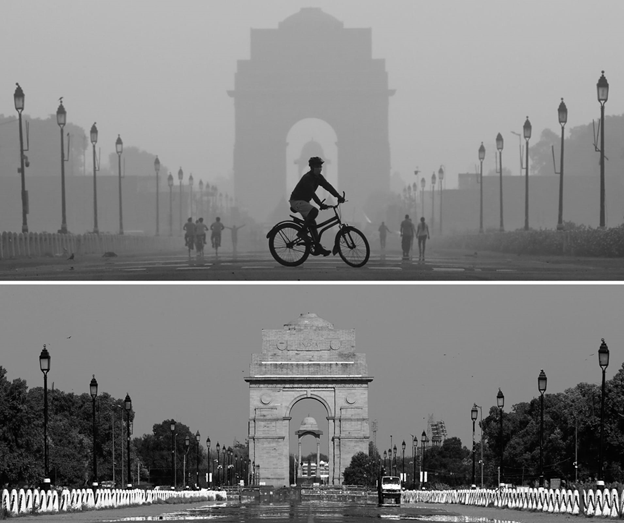
\includegraphics[width=0.6\linewidth]{images/air_pollution_greyscale} 

}

\caption{The India Gate in New Delhi, India.}\label{fig:covid}
\end{figure}

\vspace{.05in}

\begin{center}\includegraphics[width=0.6\linewidth]{12-A17-paired-simulation_files/figure-latex/unnamed-chunk-2-1} \end{center}

\vspace{.2in}

\begin{longtable}[]{@{}ccll@{}}
\caption{Summary statistics for current AQI scores, median AQI scores from 2015--2019, and the differences in AQI scores.}\tabularnewline
\toprule
& Mean & Standard deviation & Sample size \\
\midrule
\endfirsthead
\toprule
& Mean & Standard deviation & Sample size \\
\midrule
\endhead
Current & \(\bar{x}_1\) = 47.394 & \(s_1\) = 14.107 & \(n_1\) = 33 \\
5 Year Median & \(\bar{x}_2\) = 51.545 & \(s_2\) = 17.447 & \(n_2\) = 33 \\
Differences & \(\bar{x}_d\) = \(-4.152\) & \(s_d\) = 17.096 & \(n_d\) = 33 \\
\bottomrule
\end{longtable}

\newpage

\hypertarget{vocabulary-review.-4}{%
\subsubsection*{Vocabulary review.}\label{vocabulary-review.-4}}
\addcontentsline{toc}{subsubsection}{Vocabulary review.}

\begin{enumerate}
\def\labelenumi{\arabic{enumi}.}
\tightlist
\item
  What is the sample size?
\end{enumerate}

\vspace{0.3in}

\begin{enumerate}
\def\labelenumi{\arabic{enumi}.}
\setcounter{enumi}{1}
\tightlist
\item
  Identify the variables in this study. What role (explanatory or response) do each have?
\end{enumerate}

\vspace{.5in}

\begin{enumerate}
\def\labelenumi{\arabic{enumi}.}
\setcounter{enumi}{2}
\tightlist
\item
  Are the differences in AQI scores independent for each case (US city)? Explain.
\end{enumerate}

\vspace{0.5in}

\begin{enumerate}
\def\labelenumi{\arabic{enumi}.}
\setcounter{enumi}{3}
\tightlist
\item
  Why is this treated as a paired study design and not two independent samples?
\end{enumerate}

\vspace{0.5in}

\begin{enumerate}
\def\labelenumi{\arabic{enumi}.}
\setcounter{enumi}{4}
\tightlist
\item
  Is this an experiment or observational study? Justify your answer.
\end{enumerate}

\vspace{0.5in}

\hypertarget{ask-a-research-question-2}{%
\subsubsection*{Ask a research question}\label{ask-a-research-question-2}}
\addcontentsline{toc}{subsubsection}{Ask a research question}

\begin{enumerate}
\def\labelenumi{\arabic{enumi}.}
\setcounter{enumi}{5}
\tightlist
\item
  What are the two competing possibilities to run a hypothesis test for this study?
\end{enumerate}

\vspace{0.8in}

\begin{enumerate}
\def\labelenumi{\arabic{enumi}.}
\setcounter{enumi}{6}
\tightlist
\item
  Write the null hypothesis in words.
\end{enumerate}

\vspace{0.8in}

\begin{enumerate}
\def\labelenumi{\arabic{enumi}.}
\setcounter{enumi}{7}
\tightlist
\item
  What is the research question?
\end{enumerate}

\vspace{0.8in}

\begin{enumerate}
\def\labelenumi{\arabic{enumi}.}
\setcounter{enumi}{8}
\tightlist
\item
  Write the alternative hypothesis in notation.
\end{enumerate}

\vspace{0.8in}

\hypertarget{summarize-and-visualize-the-data-2}{%
\subsubsection*{Summarize and visualize the data}\label{summarize-and-visualize-the-data-2}}
\addcontentsline{toc}{subsubsection}{Summarize and visualize the data}

\begin{enumerate}
\def\labelenumi{\arabic{enumi}.}
\setcounter{enumi}{9}
\tightlist
\item
  Report the summary statistic of interest for the data.
\end{enumerate}

\vspace{0.3in}

\begin{enumerate}
\def\labelenumi{\arabic{enumi}.}
\setcounter{enumi}{10}
\tightlist
\item
  What notation is used for the value in question 10?
\end{enumerate}

\vspace{0.3in}

\hypertarget{use-statistical-inferential-methods-to-draw-inferences-from-the-data}{%
\subsubsection*{Use statistical inferential methods to draw inferences from the data}\label{use-statistical-inferential-methods-to-draw-inferences-from-the-data}}
\addcontentsline{toc}{subsubsection}{Use statistical inferential methods to draw inferences from the data}

\hypertarget{hypothesis-test}{%
\paragraph*{Hypothesis test}\label{hypothesis-test}}
\addcontentsline{toc}{paragraph}{Hypothesis test}

To simulate the null distribution of paired sample mean differences we will use a bootstrapping method. Recall that the null distribution must be created under the assumption that the null hypothesis is true. Therefore, before bootstrapping, we will need to \emph{shift} each data point by the difference \(\mu_0 - \bar{x}_d\). This will ensure that the mean of the shifted data is \(\mu_0\) (rather than the mean of the original data, \(\bar{x}_d\)), and that the simulated null distribution will be centered at the null value.

\begin{enumerate}
\def\labelenumi{\arabic{enumi}.}
\setcounter{enumi}{11}
\tightlist
\item
  Calculate the difference \(\mu_0 - \bar{x}_d\). Will we need to shift the data up or down?
\end{enumerate}

\vspace{.7in}

\begin{enumerate}
\def\labelenumi{\arabic{enumi}.}
\setcounter{enumi}{12}
\tightlist
\item
  We will use the \texttt{paired\_test()} function in \texttt{R} (in the \texttt{catstats} package) to simulate the shifted bootstrap (null) distribution of sample mean differences and compute a p-value. Use the provided \texttt{R} script file and enter the calculated value from question 12 for \texttt{xx} to simulate the null distribution and enter the summary statistic from question 10 for \texttt{yy} to find the p-value. Highlight and run lines 1--21.
\end{enumerate}

\begin{Shaded}
\begin{Highlighting}[]
    \FunctionTok{paired\_test}\NormalTok{(}\AttributeTok{data =}\NormalTok{ Air}\SpecialCharTok{$}\NormalTok{Difference,   }\CommentTok{\# Vector of differences }
                                         \CommentTok{\# or data set with column for each group}
            \AttributeTok{shift =}\NormalTok{ xx,   }\CommentTok{\# Shift needed for bootstrap hypothesis test}
            \AttributeTok{as\_extreme\_as =}\NormalTok{ yy,  }\CommentTok{\# Observed statistic}
            \AttributeTok{direction =} \StringTok{"less"}\NormalTok{,  }\CommentTok{\# Direction of alternative}
            \AttributeTok{number\_repetitions =} \DecValTok{1000}\NormalTok{,  }\CommentTok{\# Number of simulated samples for null distribution}
            \AttributeTok{which\_first =} \DecValTok{1}\NormalTok{)  }\CommentTok{\# Not needed when using calculated differences}
\end{Highlighting}
\end{Shaded}

\newpage

\begin{enumerate}
\def\labelenumi{\arabic{enumi}.}
\setcounter{enumi}{13}
\tightlist
\item
  Sketch the null distribution created in question 13 here.
\end{enumerate}

\vspace{1.9in}

\begin{enumerate}
\def\labelenumi{\arabic{enumi}.}
\setcounter{enumi}{14}
\tightlist
\item
  Explain why the null distribution is centered at zero.
\end{enumerate}

\vspace{.5in}

\begin{enumerate}
\def\labelenumi{\arabic{enumi}.}
\setcounter{enumi}{15}
\item
  What proportion of samples are at or less than the observed sample mean difference in AQI scores for current scores minus 5 year median scores? What is the statistical term for this proportion?
  \vspace{.3in}
\item
  Interpret the p-value in the context of the problem.
  \vspace{.8in}
\item
  How much evidence does this provide for improved air quality in US cities?
  \vspace{.3in}
\item
  If evidence was found for improved air quality in US cities, could we conclude that the stay-at-home directives \emph{caused} the improvement in air quality? Explain.
  \vspace{.5in}
\end{enumerate}

\hypertarget{confidence-interval}{%
\paragraph*{Confidence interval}\label{confidence-interval}}
\addcontentsline{toc}{paragraph}{Confidence interval}

We will use the \texttt{paired\_bootstrap\_CI()} function in \texttt{R} (in the \texttt{catstats} package) to simulate the bootstrap distribution of sample mean differences and calculate a confidence interval.

\begin{enumerate}
\def\labelenumi{\arabic{enumi}.}
\setcounter{enumi}{19}
\tightlist
\item
  Write out the parameter of interest in context of the study.
\end{enumerate}

\vspace{.6in}

\begin{enumerate}
\def\labelenumi{\arabic{enumi}.}
\setcounter{enumi}{20}
\tightlist
\item
  Using the provided \texttt{R} script file, fill in the missing value at \texttt{xx} to find a 99\% bootstrap confidence interval; highlight and run lines 24--27. Report the confidence interval in interval notation.
\end{enumerate}

\begin{Shaded}
\begin{Highlighting}[]
\FunctionTok{paired\_bootstrap\_CI}\NormalTok{(}\AttributeTok{data =}\NormalTok{ Air}\SpecialCharTok{$}\NormalTok{Difference, }\CommentTok{\# Enter vector of differences}
                    \AttributeTok{number\_repetitions =} \DecValTok{1000}\NormalTok{, }\CommentTok{\# Number of bootstrap samples for CI}
                    \AttributeTok{confidence\_level =}\NormalTok{ xx,  }\CommentTok{\# Confidence level in decimal form}
                    \AttributeTok{which\_first =} \DecValTok{1}\NormalTok{)  }\CommentTok{\# Not needed when entering vector of differences}
\end{Highlighting}
\end{Shaded}

\vspace{.5in}

\hypertarget{communicate-the-results-and-answer-the-research-question-2}{%
\subsubsection*{Communicate the results and answer the research question}\label{communicate-the-results-and-answer-the-research-question-2}}
\addcontentsline{toc}{subsubsection}{Communicate the results and answer the research question}

\begin{enumerate}
\def\labelenumi{\arabic{enumi}.}
\setcounter{enumi}{21}
\tightlist
\item
  Interpret the 99\% confidence interval in the context of the problem.
\end{enumerate}

\vspace{1in}

\begin{enumerate}
\def\labelenumi{\arabic{enumi}.}
\setcounter{enumi}{22}
\tightlist
\item
  Do the results of your confidence interval and hypothesis test agree? What does each tell you about the null hypothesis?
\end{enumerate}

\vspace{.7in}

\hypertarget{take-home-messages-17}{%
\subsection{Take-home messages}\label{take-home-messages-17}}

\begin{enumerate}
\def\labelenumi{\arabic{enumi}.}
\item
  The differences in a paired data set are treated like a single quantitative variable when performing a statistical analysis. Paired data (or paired samples) occur when pairs of measurements are collected. We are only interested in the population (and sample) of differences, and not in the original data.
\item
  When using bootstrapping to create a null distribution centered at the null value for both paired data and a single quantitative variable, we first need to shift the data by the difference \(\mu_0 - \bar{x}_d\), and then sample with replacement from the shifted data.
\item
  When analyzing paired data, the summary statistic is the `mean difference' NOT the `difference in means'\footnote{Technically, if we calculate the differences and then take the mean (mean difference), and we calculate the two means and then take the difference (difference in means), the value will be the same. However, the \emph{sampling variability} of the two statistics will differ, as we will see in Activity 11.}. This terminology will be \emph{very} important in interpretations.
\item
  To create one simulated sample on the null distribution for a sample mean or mean difference, shift the original data by adding \((\mu_0 - \bar{x})\) or \((0 - \bar{x}_d)\). Sample with replacement from the shifted data \(n\) times. Calculate and plot the sample mean or the sample mean difference.
\item
  To create one simulated sample on the bootstrap distribution for a sample mean or mean difference, label \(n\) cards with the original response values. Randomly draw with replacement \(n\) times. Calculate and plot the resampled mean or the resampled mean difference.
\end{enumerate}

\hypertarget{additional-notes-16}{%
\subsection{Additional notes}\label{additional-notes-16}}

Use this space to summarize your thoughts and take additional notes on today's activity and material covered.

\newpage

\hypertarget{activity-12b-construction-costs}{%
\section{Activity 12b: Construction Costs}\label{activity-12b-construction-costs}}

\setstretch{1}

\hypertarget{learning-outcomes-7}{%
\subsection{Learning outcomes}\label{learning-outcomes-7}}

\begin{itemize}
\item
  Given a research question involving paired differences, construct the null and alternative hypotheses
  in words and using appropriate statistical symbols.
\item
  Describe and perform a theory-based hypothesis test for a paired mean difference.
\item
  Interpret and evaluate a p-value for a theory-based hypothesis test for a paired mean difference.
\item
  Use theory-based methods to find a confidence interval for a paired mean difference.
\item
  Interpret a confidence interval for a paired mean difference.
\item
  Use a confidence interval to determine the conclusion of a hypothesis test.
\end{itemize}

\hypertarget{terminology-review-19}{%
\subsection{Terminology review}\label{terminology-review-19}}

In this week's activity, we will analyze paired quantitative data using simulation-based methods. Some terms covered in this activity are:

\begin{itemize}
\item
  Mean difference
\item
  Paired data
\item
  Independent groups
\item
  Shifted bootstrap (null) distribution
\end{itemize}

To review these concepts, see Section 6.2 in the textbook.

\hypertarget{out-of-class-activity}{%
\subsection{Out-of-class activity}\label{out-of-class-activity}}

The remaining questions cover theory-based methods for testing and estimating a paired mean difference (or single mean). Use Section 6.2.3 in the textbook and the OneMeanTheory video to complete the following questions.

The sampling distribution for \(\bar{x}\) based on a sample of size \(n\) from a population with a true mean \(\mu\) and true standard deviation \(\sigma\) can be modeled using a normal distribution when certain conditions are met.

Conditions for the sampling distribution of \(\bar{x}\) to follow an approximate normal distribution:

\begin{itemize}
\item
  \textbf{Independence}: The sample's observations are independent
\item
  \textbf{Normality}: The data should be approximately normal or the sample size should be large.

  \begin{itemize}
  \item
    \(n < 30\): If the sample size \(n\) is less than 30 and there are no clear outliers in the data, then we typically assume the data come from a nearly normal distribution to satisfy the condition.
  \item
    \(n \geq 30\): If the sample size \(n\) is at least 30 and there are no particularly extreme outliers, then we typically assume the sampling distribution of \(\bar{x}\) is nearly normal, even if the underlying distribution of individual observations is not.
  \end{itemize}
\end{itemize}

\begin{enumerate}
\def\labelenumi{\arabic{enumi}.}
\tightlist
\item
  In the in-class activity, we verified that the independence condition was satisfied. Is the normality condition met to use the theory-based methods for analysis? Explain your answer.
\end{enumerate}

\vspace{1in}

To find the standardized statistic for the paired differences we will use the following formula:

\[T = \frac{\bar{x}_d}{SE(\bar{x}_d)},\]

where the standard error of the sample mean difference is:

\[SE(\bar{x}_d)=\frac{s_d}{\sqrt{n}}.\]

\begin{enumerate}
\def\labelenumi{\arabic{enumi}.}
\setcounter{enumi}{1}
\tightlist
\item
  Calculate the standard error of the sample mean difference.
\end{enumerate}

\vspace{0.5in}

\begin{enumerate}
\def\labelenumi{\arabic{enumi}.}
\setcounter{enumi}{2}
\tightlist
\item
  Calculate the standardized statistic.
\end{enumerate}

\vspace{0.5in}

Using the provided \texttt{R} script file, enter the T-score (for \texttt{xx}) into the \texttt{pt()} function using a \texttt{df} = \(n_d-1 = 33 - 1 = 32\), and \texttt{lower.tail\ =\ TRUE} to find the p-value. Highlight and run line 31.

\begin{Shaded}
\begin{Highlighting}[]
\FunctionTok{pt}\NormalTok{(xx, }\AttributeTok{df=}\DecValTok{32}\NormalTok{, }\AttributeTok{lower.tail=}\ConstantTok{TRUE}\NormalTok{)}
\end{Highlighting}
\end{Shaded}

\begin{enumerate}
\def\labelenumi{\arabic{enumi}.}
\setcounter{enumi}{3}
\tightlist
\item
  Is the p-value found using theory-based methods similar to the simulation p-value found in the in-class activity?
\end{enumerate}

\vspace{0.5in}

To calculate the 99\% theory-based confidence interval for the paired mean difference, use the following formula:

\[\bar{x}_d\pm t^* SE(\bar{x}_d).\]

We will need to find the \(t^*\) multiplier using the function \texttt{qt()}. For a 99\% confidence level, we are finding the \(t^*\) value at the 99.5th percentile with \texttt{df} = \(n_d - 1 = 33 - 1 = 32\).

\begin{Shaded}
\begin{Highlighting}[]
\FunctionTok{qt}\NormalTok{(}\FloatTok{0.995}\NormalTok{, }\AttributeTok{df =} \DecValTok{32}\NormalTok{, }\AttributeTok{lower.tail=}\ConstantTok{TRUE}\NormalTok{)}
\CommentTok{\#\textgreater{} [1] 2.738481}
\end{Highlighting}
\end{Shaded}

\begin{enumerate}
\def\labelenumi{\arabic{enumi}.}
\setcounter{enumi}{4}
\tightlist
\item
  Calculate the 99\% confidence interval for the paired mean difference using theory-based methods.
\end{enumerate}

\vspace{1in}

\begin{enumerate}
\def\labelenumi{\arabic{enumi}.}
\setcounter{enumi}{5}
\tightlist
\item
  Explain why the theory-based and simulation confidence intervals are not quite the same.
\end{enumerate}

\vspace{1in}

\newpage

\hypertarget{week-12-lab-swearing}{%
\section{Week 12 Lab: Swearing}\label{week-12-lab-swearing}}

\setstretch{1}

\hypertarget{learning-objectives-18}{%
\subsection{Learning objectives}\label{learning-objectives-18}}

\newpage

\begin{enumerate}
\def\labelenumi{\arabic{enumi}.}
\setcounter{enumi}{23}
\tightlist
\item
  Write a paragraph summarizes the results of this study as if you were describing the results to your roommate. Be sure to describe:
\end{enumerate}

\begin{itemize}
\item
  Summary statistic
\item
  P-value and interpretation
\item
  Conclusion (written to answer the research question)
\item
  Confidence interval and interpretation
\item
  Scope of inference
\end{itemize}

\vspace{2.6in}

\hypertarget{inference-for-a-quantitative-response-with-independent-samples}{%
\chapter{Inference for a Quantitative Response with Independent Samples}\label{inference-for-a-quantitative-response-with-independent-samples}}

\hypertarget{reading-guide-inference-for-a-difference-in-two-means}{%
\section{Reading Guide: Inference for a Difference in Two Means}\label{reading-guide-inference-for-a-difference-in-two-means}}

\hypertarget{section-6.3-inference-for-a-difference-in-two-means}{%
\subsection*{Section 6.3 (Inference for a difference in two means)}\label{section-6.3-inference-for-a-difference-in-two-means}}
\addcontentsline{toc}{subsection}{Section 6.3 (Inference for a difference in two means)}

\textbf{Videos}

\begin{itemize}
\tightlist
\item
  6.3
\end{itemize}

\setstretch{1.25}

\hypertarget{reminders-from-previous-sections-6}{%
\subsubsection*{Reminders from previous sections}\label{reminders-from-previous-sections-6}}
\addcontentsline{toc}{subsubsection}{Reminders from previous sections}

\(n_1\)= sample size of group 1

\(n_2\) = sample size of group 2

\(\overline{x}\) = sample mean

\(s\) = sample standard deviation

\(\mu\) = population mean

\(\sigma\) = population standard deviation

General steps of a hypothesis test:

\begin{enumerate}
\def\labelenumi{\arabic{enumi}.}
\item
  Frame the research question in terms of hypotheses.
\item
  Collect and summarize data using a test statistic.
\item
  Assume the null hypothesis is true, and simulate or mathematically model a null distribution for the test statistic.
\item
  Compare the observed test statistic to the null distribution to calculate a p-value.
\item
  Make a conclusion based on the p-value and write the conclusion in context.
\end{enumerate}

Parameter: a value summarizing a variable(s) for a population.

Statistic: a value summarizing a variable(s) for a sample.

Sampling distribution: plot of statistics from 1000s of samples of the same size taken from the same population.

Standard deviation of a statistic: the variability of statistics from 1000s of samples; how far, on average, each statistic is from the true value of the parameter.

Standard error of a statistic: estimated standard deviation of a statistic.

Hypothesis test: a process to determine how strong the evidence of an effect is. Also called a `significance test.'

Simulation-based method: Simulate lots of samples of size \(n\) under assumption of the null hypothesis, then find the proportion of the simulations that are at least as extreme as the observed sample statistic.

Theory-based method: Develop a mathematical model for the sampling distribution of the statistic under the null hypothesis and use the model to calculate the probability of the observed sample statistic (or one more extreme) occurring.

Null hypothesis (\(H_0\)): the skeptical perspective; no difference; no change; no effect; random chance; what the researcher hopes to prove is \textbf{wrong}.

Alternative hypothesis (\(H_A\)): the new perspective; a difference/increase/decrease; an effect; not random chance; what the researcher hopes to prove is \textbf{correct}.

Null value: the value of the parameter when we assume the null hypothesis is true (labeled as \(parameter_0\)).

Null distribution: the simulated or modeled distribution of statistics (sampling distribution) we would expect to occur if the null hypothesis is true.

P-value: probability of seeing the observed sample data, or something more extreme, assuming the null hypothesis is true.

\(\implies\) Lower the p-value the stronger the evidence AGAINST the null hypothesis and FOR the alternative hypothesis.

Decision: a determination of whether to reject or fail to reject a null hypothesis based on a p-value and a pre-set level of significance.

\begin{itemize}
\item
  If p-value \(\leq \alpha\), then reject \(H_0\).
\item
  If p-value \(> \alpha\), then fail to reject \(H_0\).
\end{itemize}

Significance level (\(\alpha\)): a threshold used to determine if a p-value provides enough evidence to reject the null hypothesis or not.

\rgi Common levels of \(\alpha\) include 0.01, 0.05, and 0.10.

Statistically significant: results are considered statistically significant if the p-value is below the significance level.

Confidence interval: a process to determine how large an effect is; a range of plausible values for the parameter. Also called `estimation.'

Margin of error: the value that is added to and subtracted from the sample statistic to create a confidence interval; half the width of a confidence interval.

Bootstrapping: the process of drawing with replacement \(n\) times from the original sample.

Bootstrapped resample: a random sample of size \(n\) from the original sample, selected with replacement.

Bootstrapped statistic: the statistic recorded from the bootstrapped resample.

Confidence level: how confident we are that the confidence interval will capture the parameter.

Bootstrap \(X\)\% confidence interval: (\((\frac{(1-X)}{2})^{th}\) percentile, \((X+(\frac{(1-X)}{2})^{th}\) percentile) of a bootstrap distribution.

Central Limit Theorem: For large sample sizes, the sampling distribution of a sample mean (or proportion) will be approximately normal (bell-shaped and symmetric).

\(t\)-distribution: A bell-shaped symmetric distribution, centered at 0, wider than the standard normal distribution.

\begin{itemize}
\tightlist
\item
  The variability in a \(t\)-distribution depends on the sample size (used to calculate degrees of freedom --- df for short).
\item
  The \(t\)-distribution gets closer to the standard normal distribution as df increases.
\end{itemize}

Degrees of freedom (df): describes the variability of the \(t\)-distribution.

T-score: the name for a standardized statistic which is compared to a \(t\)-distribution.

\hypertarget{notes-24}{%
\subsubsection*{Notes}\label{notes-24}}
\addcontentsline{toc}{subsubsection}{Notes}

To create a \textbf{simulated null distribution} of differences in sample means,

\begin{enumerate}
\def\labelenumi{\arabic{enumi}.}
\item
  How many cards will you need and how will the cards be labeled?
  \rgs
\item
  What do you do with the cards after labeling them?
  \rgs
\item
  After shuffling, what value will be plotted on the simulated null distribution?
  \rgs
\end{enumerate}

To create a \textbf{bootstrap distribution} of differences in sample means,

\begin{enumerate}
\def\labelenumi{\arabic{enumi}.}
\item
  How many cards will you need and how will the cards be labeled?
  \rgs
\item
  What do you do with the cards after labeling them?
  \rgs
\item
  After shuffling, what value will be plotted on the bootstrap distribution?
  \rgs
\end{enumerate}

Conditions to use the CLT for a difference in two means:

\rgi Independence:
\rgs

\rgi \rgi Checked by:
\rgs

\rgi Normality:
\rgs

\rgi \rgi Checked by:
\rgs

In a two-sample \(t\)-test, how are the degrees of freedom determined?
\rgs        

True or false: A large p-value indicates that the null hypothesis is true.
\rgs

\hypertarget{formulas-7}{%
\subsubsection*{Formulas}\label{formulas-7}}
\addcontentsline{toc}{subsubsection}{Formulas}

\(SE(\overline{x_1} - \overline{x_2})=\)
\rgs

\(T=\)
\rgs

Confidence interval for a difference in means:
\rgs

\hypertarget{notation-4}{%
\subsubsection*{Notation}\label{notation-4}}
\addcontentsline{toc}{subsubsection}{Notation}

\(\mu_1\) represents
\rgs

\(\mu_2\) represents
\rgs

\(\sigma_1\) represents
\rgs

\(\sigma_2\) represents
\rgs

\(\overline{x_1}\) represents
\rgs

\(\overline{x_2}\) represents
\rgs

\(s_1\) represents
\rgs

\(s_2\) represents
\rgs

\hypertarget{example-test-scores}{%
\subsubsection*{Example: Test scores}\label{example-test-scores}}
\addcontentsline{toc}{subsubsection}{Example: Test scores}

\begin{enumerate}
\def\labelenumi{\arabic{enumi}.}
\item
  What are the observational units?
  \rgs
\item
  What are the sample statistics presented in this example? What notation would be used to represent each value?
  \rgs
\item
  What is the parameter representing in the context of this problem? What notation would be used to represent this parameter?
  \rgs
  \rgs
\item
  What is the research question?
  \rgs
\item
  Write the null and alternative hypothesis in appropriate notation.
  \rgs
\item
  How could we use cards to simulate \textbf{one} sample \emph{which assumes the null hypothesis is true}? How many cards? What is written on the cards? What would we do with the cards? What would you record once you have a simulated sample?
  \rgs
  \rgs
  \rgs
\item
  After 1000 shuffles are generated, where is the resulting simulated distribution centered? Why does that make sense?
  \rgs
  \rgs
\item
  How was the p-value for this test found? The proportion of simulated null samples at \_\_\_\_ or \_\_\_\_\_\_\_\_\_\_\_.
  \rgs
\item
  Interpret the p-value in the context of the problem.
  \rgs
  \rgs
\item
  From these data, can we conclude the exams are equally difficult?
  \rgs
\item
  What type of error may have occurred at the 5\% significance level? Interpret that error in context.
  \rgs
  \rgs
\end{enumerate}

\hypertarget{example-esc-and-heart-attacks}{%
\subsubsection*{Example: ESC and heart attacks}\label{example-esc-and-heart-attacks}}
\addcontentsline{toc}{subsubsection}{Example: ESC and heart attacks}

\begin{enumerate}
\def\labelenumi{\arabic{enumi}.}
\item
  What is the research question?
  \rgs
\item
  What are the observational units?
  \rgs
\item
  What variables are recorded? Give the type (categorical or quantitative) and role (explanatory or response) of each.
  \rgs
  \rgs
\item
  What are the sample statistics presented in this example? What notation would be used to represent each value?
  \rgs
\item
  What is the parameter representing in the context of this problem? What notation would be used to represent this parameter?
  \rgs
  \rgs
\item
  How could we use cards to simulate \textbf{one} bootstrap resample \emph{which does not assume the null hypothesis is true}? How many cards? What is written on the cards? What would we do with the cards? What would you record once you have a simulated sample?
  \rgs
  \rgs
  \rgs
\item
  After 1000 resamples are generated, where is the resulting bootstrap distribution centered? Why does that make sense?
  \rgs
  \rgs
\item
  Does the 90\% confidence interval provide evidence of a difference across the two treatments?
  \rgs
  \rgs
\end{enumerate}

\hypertarget{example-nc-births}{%
\subsubsection*{Example: NC births}\label{example-nc-births}}
\addcontentsline{toc}{subsubsection}{Example: NC births}

\begin{enumerate}
\def\labelenumi{\arabic{enumi}.}
\item
  What is the research question?
  \rgs
\item
  What are the observational units?
  \rgs
\item
  What variables will be analyzed? Give the type and role of each.
  \rgs
  \rgs
\item
  Can the results of this study be generalized to a larger population?
  \rgs
\item
  Are causal conclusions appropriate for these data?
  \rgs
\item
  Write the null and the alternative hypotheses in words.
  \rgs
  \rgs
\item
  Write the null and the alternative hypotheses in notation.
  \rgs
\item
  What are the sample statistics presented in this example? What notation would be used to represent each value?
  \rgs
\item
  Are the independence and normality conditions satisfied?
  \rgs
  \rgs
\item
  Calculate the standard error of the difference in sample means.
  \rgs
  \rgs
\item
  Calculate the T-score (the standardized statistic for the sample mean).
  \rgs
  \rgs
\item
  What distribution should the T-score be compared to in order to calculate a p-value?
  \rgs
\item
  What was the p-value of the test?
  \rgs
\item
  What conclusion should the researcher make?
  \rgs
  \rgs
\item
  Calculate a 95\% confidence interval for the parameter of interest using \texttt{qt(0.975,\ df\ =\ 49)\ =\ 1.677} as the \(t^\star\) value.
  \rgs
  \rgs
\item
  Interpret your interval in the context of the problem.
  \rgs
  \rgs
\end{enumerate}

\newpage

\hypertarget{week-13---activity-13a-weather-patterns-and-record-snowfall}{%
\section{Week 13 - Activity 13a: Weather Patterns and Record Snowfall}\label{week-13---activity-13a-weather-patterns-and-record-snowfall}}

\setstretch{1}

\hypertarget{learning-objectives-19}{%
\subsection{Learning objectives}\label{learning-objectives-19}}

\begin{itemize}
\item
  Given a research question involving one categorical explanatory variable and one quantitative response variable, construct the null and alternative hypotheses
  in words and using appropriate statistical symbols.
\item
  Describe and perform a simulation-based hypothesis test for a difference in means.
\item
  Interpret and evaluate a p-value for a simulation-based hypothesis test for a difference in means.
\item
  Use bootstrapping to find a confidence interval for a difference in means.
\item
  Interpret a confidence interval for a difference in means.
\item
  Use a confidence interval to determine the conclusion of a hypothesis test.
\end{itemize}

\hypertarget{terminology-review-20}{%
\subsection{Terminology review}\label{terminology-review-20}}

In today's activity, we will use simulation-based methods to analyze the association between one categorical explanatory variable and one quantitative response variable, where the groups formed by the categorical variable are independent. Some terms covered in this activity are:

\begin{itemize}
\item
  Independent groups
\item
  Difference in means
\end{itemize}

To review these concepts, see Section 6.3 in the textbook.

\hypertarget{weather-patterns-and-record-snowfall}{%
\subsection{Weather patterns and record snowfall}\label{weather-patterns-and-record-snowfall}}

In the winter of 2018--2019, Bozeman had a record snowfall which resulted in the collapse of two flat-roofed buildings on the MSU campus. A writer for the \emph{Washington Post} predicted the heavy snowfall for 2018--2019 due to the El Ni\latexcode{\~{n}}o weather pattern that occurred in that season. A meteorologist in Montana wanted to see if the weather pattern really was associated with total snowfall. She obtained historical data from 44 years on the weather pattern (El Ni\latexcode{\~{n}}o or La Ni\latexcode{\~{n}}a) and snowfall (in inches) at the Billings Weather Station. Side-by-side boxplots and summary statistics for each group are shown on the following page.

Notice from the \texttt{R} code that the name of the data set is \texttt{Snow}.

\begin{Shaded}
\begin{Highlighting}[]
\CommentTok{\# Read in data set}
\NormalTok{Snow }\OtherTok{\textless{}{-}} \FunctionTok{read.csv}\NormalTok{(}\StringTok{"https://math.montana.edu/courses/s216/data/SnowfallByWeatherPattern.csv"}\NormalTok{)}

\CommentTok{\# Code categorical variables as factors}
\NormalTok{Snow }\OtherTok{\textless{}{-}} \CommentTok{\# Write over original data with the following}
\NormalTok{  Snow }\SpecialCharTok{\%\textgreater{}\%} \CommentTok{\# Pipe data set into}
  \FunctionTok{mutate}\NormalTok{(}\AttributeTok{WeatherPattern =} \FunctionTok{factor}\NormalTok{(WeatherPattern)) }\CommentTok{\# Convert to factor}
\end{Highlighting}
\end{Shaded}

\newpage

\begin{Shaded}
\begin{Highlighting}[]
\CommentTok{\# Side{-}by{-}side box plots}
\NormalTok{Snow }\SpecialCharTok{\%\textgreater{}\%}
\FunctionTok{ggplot}\NormalTok{(}\FunctionTok{aes}\NormalTok{(}\AttributeTok{x =}\NormalTok{ WeatherPattern, }\AttributeTok{y =}\NormalTok{ Snowfall)) }\SpecialCharTok{+}
    \FunctionTok{geom\_boxplot}\NormalTok{() }\SpecialCharTok{+} 
    \FunctionTok{labs}\NormalTok{(}\AttributeTok{title =} \StringTok{"Snowfall by weather pattern"}\NormalTok{,}
         \AttributeTok{x =} \StringTok{"Weather pattern"}\NormalTok{) }\SpecialCharTok{+}
    \FunctionTok{coord\_flip}\NormalTok{()}
\end{Highlighting}
\end{Shaded}

\begin{center}\includegraphics[width=0.6\linewidth]{13-A19-inference-1ofeach-simulation_files/figure-latex/unnamed-chunk-2-1} \end{center}

\begin{Shaded}
\begin{Highlighting}[]
\CommentTok{\# Summary statistics}
\NormalTok{Snow }\SpecialCharTok{\%\textgreater{}\%} 
     \FunctionTok{summarize}\NormalTok{(}\FunctionTok{favstats}\NormalTok{(Snowfall }\SpecialCharTok{\textasciitilde{}}\NormalTok{ WeatherPattern))}
\end{Highlighting}
\end{Shaded}

\begin{verbatim}
#>   WeatherPattern  min   Q1 median   Q3   max     mean       sd  n missing
#> 1        El_Nino 31.9 46.4   57.7 64.3  87.9 56.23043 13.00823 23       0
#> 2        La_Nina 44.5 51.4   60.9 70.3 107.2 63.13333 15.48626 21       0
\end{verbatim}

\hypertarget{quantitative-variables-review.}{%
\subsubsection*{Quantitative variables review.}\label{quantitative-variables-review.}}
\addcontentsline{toc}{subsubsection}{Quantitative variables review.}

\begin{enumerate}
\def\labelenumi{\arabic{enumi}.}
\tightlist
\item
  The two variables assessed in this study are the type of weather pattern and snowfall. Identify the role for each variable (explanatory or response).
\end{enumerate}

\vspace{.6in}

\begin{enumerate}
\def\labelenumi{\arabic{enumi}.}
\setcounter{enumi}{1}
\tightlist
\item
  Which group (El Ni\latexcode{\~{n}}o or La Ni\latexcode{\~{n}}a) has the highest center in the distributions of snowfall? Explain which measure of center you are using.
\end{enumerate}

\vspace{.6in}

\begin{enumerate}
\def\labelenumi{\arabic{enumi}.}
\setcounter{enumi}{2}
\tightlist
\item
  Using the side-by-side box plots, which group has the largest spread in snowfall? How did you make that choice?
\end{enumerate}

\vspace{.6in}

\newpage

\begin{enumerate}
\def\labelenumi{\arabic{enumi}.}
\setcounter{enumi}{3}
\tightlist
\item
  Is this an experiment or an observational study? Justify your answer.
\end{enumerate}

\vspace{1in}

\begin{enumerate}
\def\labelenumi{\arabic{enumi}.}
\setcounter{enumi}{4}
\tightlist
\item
  Is this a paired data set or two independent groups? Explain your reasoning.
\end{enumerate}

\vspace{1in}

\hypertarget{ask-a-research-question-3}{%
\subsubsection*{Ask a research question}\label{ask-a-research-question-3}}
\addcontentsline{toc}{subsubsection}{Ask a research question}

\begin{enumerate}
\def\labelenumi{\arabic{enumi}.}
\setcounter{enumi}{5}
\tightlist
\item
  Write out the parameter of interest in context of the study. Use proper notation and be sure to define your subscripts. Use El Ni\latexcode{\~{n}}o minus La Ni\latexcode{\~{n}}a as the order of subtraction.
\end{enumerate}

\vspace{1in}

\begin{enumerate}
\def\labelenumi{\arabic{enumi}.}
\setcounter{enumi}{6}
\tightlist
\item
  What are the two competing possibilities we will evaluate in this study?
\end{enumerate}

\vspace{1in}

\begin{enumerate}
\def\labelenumi{\arabic{enumi}.}
\setcounter{enumi}{7}
\tightlist
\item
  Identify which of your answers in question 7 is the null hypothesis and which is the alternative hypothesis.
\end{enumerate}

\vspace{1in}

\hypertarget{summarize-and-visualize-the-data-3}{%
\subsubsection*{Summarize and visualize the data}\label{summarize-and-visualize-the-data-3}}
\addcontentsline{toc}{subsubsection}{Summarize and visualize the data}

\begin{enumerate}
\def\labelenumi{\arabic{enumi}.}
\setcounter{enumi}{8}
\tightlist
\item
  Calculate the summary statistic of interest. Use El Ni\latexcode{\~{n}}o minus La Ni\latexcode{\~{n}}a as the order of subtraction. What is the appropriate notation for this statistic?
\end{enumerate}

\vspace{0.5in}

\newpage

\hypertarget{use-statistical-inferential-methods-to-draw-inferences-from-the-data-1}{%
\subsubsection*{Use statistical inferential methods to draw inferences from the data}\label{use-statistical-inferential-methods-to-draw-inferences-from-the-data-1}}
\addcontentsline{toc}{subsubsection}{Use statistical inferential methods to draw inferences from the data}

\hypertarget{hypothesis-test-1}{%
\paragraph*{Hypothesis test}\label{hypothesis-test-1}}
\addcontentsline{toc}{paragraph}{Hypothesis test}

Remember that the null distribution is created based on the assumption the null hypothesis is true. In this study, the null hypothesis states that there is no association between the two variables. This means that the snowfall values observed in the data set would have been the same regardless of the weather pattern that year.

To demonstrate this simulation, your instructor will use cards to represent the sample.

\begin{enumerate}
\def\labelenumi{\arabic{enumi}.}
\setcounter{enumi}{9}
\tightlist
\item
  How many cards will we start with?
\end{enumerate}

\vspace{0.3in}

\begin{enumerate}
\def\labelenumi{\arabic{enumi}.}
\setcounter{enumi}{10}
\tightlist
\item
  What will we write on each card?
\end{enumerate}

\vspace{0.3in}

\begin{enumerate}
\def\labelenumi{\arabic{enumi}.}
\setcounter{enumi}{11}
\tightlist
\item
  Next, we will mix the cards together and shuffle into two piles. How many cards will go into each pile? What should we label the piles?
\end{enumerate}

\vspace{.8in}

\begin{enumerate}
\def\labelenumi{\arabic{enumi}.}
\setcounter{enumi}{12}
\tightlist
\item
  What value is calculated from the cards and plotted on the null distribution? \emph{Hint}: What statistic are we calculating from the data?
\end{enumerate}

\vspace{0.3in}

\begin{enumerate}
\def\labelenumi{\arabic{enumi}.}
\setcounter{enumi}{13}
\tightlist
\item
  Once we create a null distribution of 1000 simulations, at what value do you expect the distribution to be centered? Explain your reasoning.
\end{enumerate}

\vspace{.8in}

We will use the \texttt{two\_mean\_test()} function in \texttt{R} (in the \texttt{catstats} package) to simulate the null distribution of differences in sample means and compute a p-value.

\begin{enumerate}
\def\labelenumi{\arabic{enumi}.}
\setcounter{enumi}{14}
\tightlist
\item
  When using the \texttt{two\_mean\_test()} function, we need to enter the name of the response variable, \texttt{Snowfall}, and the name of the explanatory variable, \texttt{WeatherPattern}, for the formula. The name of the data set as shown above is \texttt{Snow}. What values should be entered for each of the following to create 1000 simulated samples?
\end{enumerate}

\newpage

\begin{itemize}
\tightlist
\item
  First in subtraction (What is the outcome for the explanatory variable that is used as first in the order of subtraction? \texttt{"El\_Nino"} or \texttt{"La\_Nina"}):
\end{itemize}

\vspace{.2in}

\begin{itemize}
\tightlist
\item
  Number of repetitions:
\end{itemize}

\vspace{.2in}

\begin{itemize}
\tightlist
\item
  As extreme as:
\end{itemize}

\vspace{.2in}

\begin{itemize}
\tightlist
\item
  Direction (\texttt{"greater"}, \texttt{"less"}, or \texttt{"two-sided"}):
\end{itemize}

\vspace{.2in}

\begin{enumerate}
\def\labelenumi{\arabic{enumi}.}
\setcounter{enumi}{15}
\tightlist
\item
  Simulate a null distribution and compute the p-value. Using the \texttt{R} script file for this activity, enter your answers for question 15 in place of the \texttt{xx}'s to produce the null distribution with 1000 simulations. Highlight and run lines 1--29.
\end{enumerate}

\begin{Shaded}
\begin{Highlighting}[]
\FunctionTok{two\_mean\_test}\NormalTok{(Snowfall }\SpecialCharTok{\textasciitilde{}}\NormalTok{ WeatherPattern, }\AttributeTok{data =}\NormalTok{ Snow,  }\CommentTok{\# Variables and data}
         \AttributeTok{first\_in\_subtraction =} \StringTok{"xx"}\NormalTok{, }\CommentTok{\# First outcome in order of subtraction}
         \AttributeTok{number\_repetitions =} \DecValTok{1000}\NormalTok{,  }\CommentTok{\# Number of simulations}
         \AttributeTok{as\_extreme\_as =}\NormalTok{ xx,  }\CommentTok{\# Observed statistic}
         \AttributeTok{direction =} \StringTok{"xx"}\NormalTok{)  }\CommentTok{\# Direction of alternative: "greater", "less", or "two{-}sided"}
\end{Highlighting}
\end{Shaded}

~~~~~~~Sketch the null distribution created using the code above.

\vspace{1.5in}

\begin{enumerate}
\def\labelenumi{\arabic{enumi}.}
\setcounter{enumi}{16}
\tightlist
\item
  Report the p-value. Based off of this p-value, write a conclusion to the hypothesis test.
\end{enumerate}

\vspace{0.9in}

\newpage

\hypertarget{confidence-interval-1}{%
\paragraph*{Confidence interval}\label{confidence-interval-1}}
\addcontentsline{toc}{paragraph}{Confidence interval}

We will use the \texttt{two\_mean\_bootstrap\_CI()} function in \texttt{R} (in the \texttt{catstats} package) to simulate the bootstrap distribution of differences in sample means and calculate a confidence interval.

\begin{enumerate}
\def\labelenumi{\arabic{enumi}.}
\setcounter{enumi}{17}
\tightlist
\item
  Using bootstrapping find a 95\% confidence interval. Using the provided \texttt{R} script file, enter the variable names and data set name as in the \texttt{two\_mean\_test()} function, outcome name for the first in subtraction, number of repetitions, and the confidence level as a decimal. Highlight and run lines 32--35. Report the 95\% confidence interval in interval notation.
\end{enumerate}

\begin{Shaded}
\begin{Highlighting}[]
\FunctionTok{two\_mean\_bootstrap\_CI}\NormalTok{(RESPONSE }\SpecialCharTok{\textasciitilde{}}\NormalTok{ EXPLANATORY, }\AttributeTok{data =}\NormalTok{ DATASET,  }\CommentTok{\# Variables and data}
                      \AttributeTok{first\_in\_subtraction =} \StringTok{"xx"}\NormalTok{, }\CommentTok{\# First value in order of subtraction}
                      \AttributeTok{number\_repetitions =} \DecValTok{1000}\NormalTok{,  }\CommentTok{\# Number of simulations}
                      \AttributeTok{confidence\_level =}\NormalTok{ xx)}
\end{Highlighting}
\end{Shaded}

\vspace{0.3in}

\begin{enumerate}
\def\labelenumi{\arabic{enumi}.}
\setcounter{enumi}{18}
\tightlist
\item
  Interpret the interval you calculated in question 18.
\end{enumerate}

\vspace{1in}

\begin{enumerate}
\def\labelenumi{\arabic{enumi}.}
\setcounter{enumi}{19}
\tightlist
\item
  Would the results from a theory-based test match the results we saw with the simulation? Explain why or why not.
\end{enumerate}

\vspace{1in}

\begin{enumerate}
\def\labelenumi{\arabic{enumi}.}
\setcounter{enumi}{21}
\tightlist
\item
  If we had data on 45 La Ni\latexcode{\~{n}}a years and 47 El Ni\latexcode{\~{n}}o years and found a similar-valued summary statistic, what would happen to the p-value? The width of the confidence interval? The power of the test?
\end{enumerate}

\vspace{1in}

\hypertarget{take-home-messages-18}{%
\subsection{Take-home messages}\label{take-home-messages-18}}

\begin{enumerate}
\def\labelenumi{\arabic{enumi}.}
\item
  This activity differs from Activities 12a and 12b because the responses are independent, not paired. These data are analyzed as a difference in means, not a mean difference.
\item
  To create one simulated sample on the null distribution for a difference in sample means, label cards with the response variable values from the original data. Mix cards together and shuffle into two new groups of sizes \(n_1\) and \(n_2\). Calculate and plot the difference in means.
\item
  To create one simulated sample on the bootstrap distribution for a difference in sample means, label \(n_1 + n_2\) cards with the original response values. Keep groups separate and randomly draw with replacement \(n_1\) times from group 1 and \(n_2\) times from group 2. Calculate and plot the resampled difference in means.
\end{enumerate}

\hypertarget{additional-notes-17}{%
\subsection{Additional notes}\label{additional-notes-17}}

Use this space to summarize your thoughts and take additional notes on today's activity and material covered

\newpage

\hypertarget{activity-13b-homeless-housing-stability}{%
\section{Activity 13b: Homeless Housing Stability}\label{activity-13b-homeless-housing-stability}}

\setstretch{1}

\hypertarget{learning-objectives-20}{%
\subsection{Learning objectives}\label{learning-objectives-20}}

\begin{itemize}
\item
  Given a research question involving one categorical explanatory variable and one quantitative response variable, construct the null and alternative hypotheses
  in words and using appropriate statistical symbols.
\item
  Describe and perform a theory-based hypothesis test for a difference in means.
\item
  Interpret and evaluate a p-value for a theory-based hypothesis test for a difference in means.
\item
  Use theory-based methods to find a confidence interval for a difference in means.
\item
  Interpret a confidence interval for a difference in means.
\item
  Use a confidence interval to determine the conclusion of a hypothesis test.
\end{itemize}

\hypertarget{terminology-review-21}{%
\subsection{Terminology review}\label{terminology-review-21}}

In today's activity, we will use theory-based methods to analyze the association between one categorical explanatory variable and one quantitative response variable, where the groups formed by the categorical variable are independent. Some terms covered in this activity are:

\begin{itemize}
\item
  Independent groups
\item
  Difference in means
\item
  Independence
\item
  Normality
\end{itemize}

To review these concepts, see Section 6.3 in the textbook.

\hypertarget{homeless-housing-stability}{%
\subsection{Homeless Housing Stability}\label{homeless-housing-stability}}

Homeless people with substance abuse disorders (SUD) have high disease risk, poor access to health care, and are frequent users of Medicaid and other social services. Low-demand supportive housing with no prerequisites for treatment or sobriety has been shown to improve housing stability and decrease public service use for chronically homeless people with serious mental illness. Researchers in New York investigated if low-demand housing would also prove beneficial to chronic homeless people with SUD who do not suffer from serious mental illness or if pre-housing SUD treatments were required to improve outcomes. Between 2007 and 2012, 1937 chronic homeless people with SUD and without serious mental illness applying for low-demand housing were recruited to participate in the study. Researchers randomly assigned 1425 participants to receive SUD treatment prior to obtaining housing, the other 512 did not undergo SUD treatment. One of several outcomes measured was the length of stay in supportive housing used as a measure of housing stability. The length of stay for treatment groups is summarized in the \texttt{R} output provided. Is there evidence that SUD treatment affects the length of stay in supportive housing?

\hypertarget{ask-a-research-question-4}{%
\subsubsection*{Ask a research question}\label{ask-a-research-question-4}}
\addcontentsline{toc}{subsubsection}{Ask a research question}

\begin{enumerate}
\def\labelenumi{\arabic{enumi}.}
\tightlist
\item
  Write out the null hypothesis in notation for this study. Be sure to clearly identify the subscripts.
\end{enumerate}

\vspace{0.5in}

\begin{enumerate}
\def\labelenumi{\arabic{enumi}.}
\setcounter{enumi}{1}
\tightlist
\item
  Write out the alternative hypothesis in words for this study.
\end{enumerate}

\vspace{0.8in}

The sampling distribution for \(\bar{x}_1-\bar{x}_2\) can be modeled using a normal distribution when certain conditions are met.

Conditions for the sampling distribution of \(\bar{x}_1-\bar{x}_2\) to follow an approximate normal distribution:

\begin{itemize}
\item
  \textbf{Independence}: The sample's observations are independent
\item
  \textbf{Normality}: Each sample should be approximately normal or have a large sample size. For \emph{each} sample:

  \begin{itemize}
  \item
    \(n < 30\): If the sample size \(n\) is less than 30 and there are no clear outliers in the data, then we typically assume the data come from a nearly normal distribution to satisfy the condition.
  \item
    \(n \ge 30\): If the sample size \(n\) is at least 30 and there are no particularly extreme outliers, then we typically assume the sampling distribution of \(\bar{x}\) is nearly normal, even if the underlying distribution of individual observations is not.
  \end{itemize}
\end{itemize}

\begin{Shaded}
\begin{Highlighting}[]
\NormalTok{SUD }\OtherTok{\textless{}{-}} \FunctionTok{read.csv}\NormalTok{(}\StringTok{"data/SUD.csv"}\NormalTok{)}
\NormalTok{SUD }\SpecialCharTok{\%\textgreater{}\%}  \CommentTok{\# Data set piped into...}
  \FunctionTok{ggplot}\NormalTok{(}\FunctionTok{aes}\NormalTok{(}\AttributeTok{y =}\NormalTok{ stay, }\AttributeTok{x =}\NormalTok{ group))}\SpecialCharTok{+}  \CommentTok{\# Identify variables}
  \FunctionTok{geom\_boxplot}\NormalTok{()}\SpecialCharTok{+}  \CommentTok{\# Tell it to make a box plot}
  \FunctionTok{labs}\NormalTok{(}\AttributeTok{title =} \StringTok{"Length of Stay for those who did and did not Undergo SUD Treatment"}\NormalTok{,  }\CommentTok{\# Title}
       \AttributeTok{x =} \StringTok{"Group"}\NormalTok{,    }\CommentTok{\# x{-}axis label}
       \AttributeTok{y =} \StringTok{"Length of Stay (days)"}\NormalTok{)  }\CommentTok{\# y{-}axis label}
\end{Highlighting}
\end{Shaded}

\begin{center}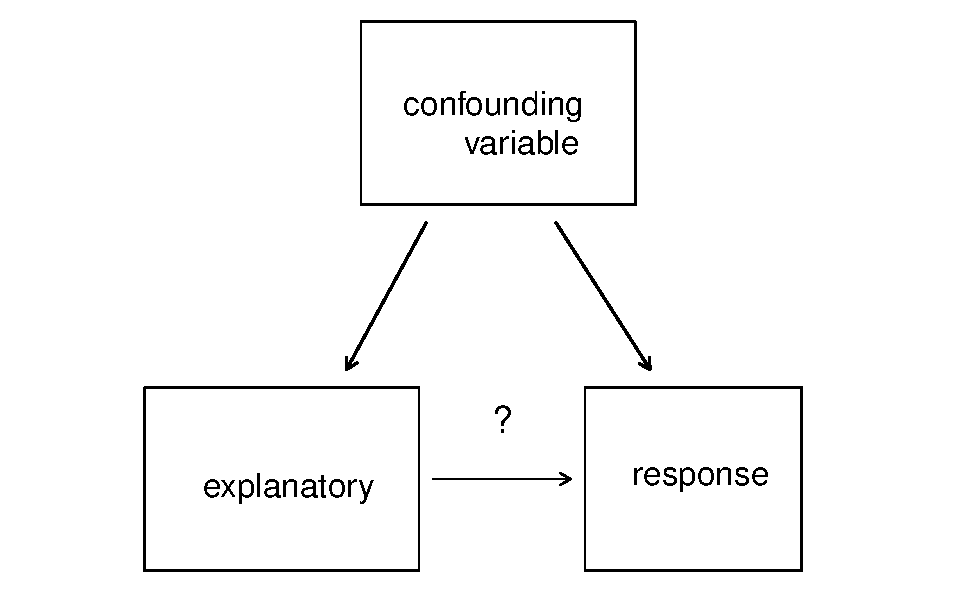
\includegraphics[width=0.7\linewidth]{13-A20-inference-1ofeach-theory_files/figure-latex/unnamed-chunk-1-1} \end{center}

The following code gives the summary statistics for the data.

\begin{Shaded}
\begin{Highlighting}[]
\NormalTok{SUD }\SpecialCharTok{\%\textgreater{}\%}
  \FunctionTok{summarize}\NormalTok{(}\FunctionTok{favstats}\NormalTok{(stay }\SpecialCharTok{\textasciitilde{}}\NormalTok{ group))}
\CommentTok{\#\textgreater{}       group min     Q1 median      Q3  max     mean       sd    n missing}
\CommentTok{\#\textgreater{} 1   treated  20 904.00   1140 1401.00 2360 1144.948 365.7267 1425       0}
\CommentTok{\#\textgreater{} 2 untreated  23 827.75   1016 1274.25 2226 1043.355 350.1818  512       0}
\end{Highlighting}
\end{Shaded}

\begin{enumerate}
\def\labelenumi{\arabic{enumi}.}
\setcounter{enumi}{2}
\item
  Is the independence condition met? Explain your answer.
  \vspace{0.4in}
\item
  Check that the normality condition is met to use theory-based methods to analyze these data.
\end{enumerate}

\vspace{0.8in}

\hypertarget{summarize-and-visualize-the-data-4}{%
\subsubsection*{Summarize and visualize the data}\label{summarize-and-visualize-the-data-4}}
\addcontentsline{toc}{subsubsection}{Summarize and visualize the data}

\begin{enumerate}
\def\labelenumi{\arabic{enumi}.}
\setcounter{enumi}{4}
\tightlist
\item
  Calculate the summary statistic for this study. Use treated minus untreated as the order of subtraction. Give the appropriate notation with cleary defined subscripts.
\end{enumerate}

\vspace{0.8in}

\hypertarget{use-statistical-inferential-methods-to-draw-inferences-from-the-data-2}{%
\subsubsection*{Use statistical inferential methods to draw inferences from the data}\label{use-statistical-inferential-methods-to-draw-inferences-from-the-data-2}}
\addcontentsline{toc}{subsubsection}{Use statistical inferential methods to draw inferences from the data}

To find the standardized statistic for the difference in means we will calculate:

\[T = \frac{\bar{x}_1-\bar{x}_2}{SE(\bar{x}_1-\bar{x}_2)},\]

where the standard error of the difference in means is calculated using:

\[SE(\bar{x}_1 -\bar{x}_2)=\sqrt{\frac{s_1^2}{n_1}+\frac{s_2^2}{n_2}}.\]

\begin{enumerate}
\def\labelenumi{\arabic{enumi}.}
\setcounter{enumi}{5}
\tightlist
\item
  Calculate the standard error for the difference in sample means.
\end{enumerate}

\vspace{0.5in}
\newpage

\begin{enumerate}
\def\labelenumi{\arabic{enumi}.}
\setcounter{enumi}{6}
\tightlist
\item
  Calculate the standardized statistic for the difference in sample means.
\end{enumerate}

\vspace{0.5in}

\begin{enumerate}
\def\labelenumi{\arabic{enumi}.}
\setcounter{enumi}{7}
\tightlist
\item
  We will use the t-distribution with degrees of freedom smallest sample size minus 1 (\texttt{df} = minimum(\(n_1 - 1, n_2 - 1\)). Calculate the \texttt{df} for this study.
\end{enumerate}

\vspace{0.2in}

\begin{enumerate}
\def\labelenumi{\arabic{enumi}.}
\setcounter{enumi}{8}
\tightlist
\item
  Using the provided \texttt{R} script file, enter the T-score (for \texttt{xx}) and the \texttt{df} calculated in question 8 for yy into the \texttt{pt()} function to find the p-value. Highlight and run line 20. Report the p-value calculated.
\end{enumerate}

\begin{Shaded}
\begin{Highlighting}[]
\DecValTok{2}\SpecialCharTok{*}\FunctionTok{pt}\NormalTok{(xx, }\AttributeTok{df=}\NormalTok{yy, }\AttributeTok{lower.tail=}\ConstantTok{TRUE}\NormalTok{)}
\end{Highlighting}
\end{Shaded}

\vspace{0.2in}

\begin{enumerate}
\def\labelenumi{\arabic{enumi}.}
\setcounter{enumi}{9}
\item
  Explain why we multiplied by 2 in the code above.
  \vspace{0.3in}
\item
  Interpret the p-value in context of the study.
  \vspace{0.8in}
\item
  Do you expect the 95\% confidence interval to contain the null value of zero? Explain your answer.
  \vspace{0.8in}
\end{enumerate}

To calculate a theory-based 95\% confidence interval for a difference in means, use the formula:

\[\bar{x}_1- \bar{x}_2\pm t^* SE(\bar{x}_1- \bar{x}_2).\]

We will need to find the \(t^*\) multiplier using the function \texttt{qt()}. For a 95\% confidence level, we are finding the \(t^*\) value at the 97.5th percentile with \texttt{df} = minimum(\(n_1 - 1, n_2 - 1\)).

Enter the appropriate percentile value (as a decimal) for xx and degrees of freedom for yy into the \texttt{qt()} function at line 23 to find the appropriate \(t^*\) multiplier

\begin{Shaded}
\begin{Highlighting}[]
\FunctionTok{qt}\NormalTok{(xx, }\AttributeTok{df =}\NormalTok{ yy, }\AttributeTok{lower.tail=}\ConstantTok{TRUE}\NormalTok{)}
\end{Highlighting}
\end{Shaded}

\begin{enumerate}
\def\labelenumi{\arabic{enumi}.}
\setcounter{enumi}{12}
\tightlist
\item
  Report the \(t^*\) multiplier for the 95\% confidence interval.
\end{enumerate}

\vspace{0.2in}

\begin{enumerate}
\def\labelenumi{\arabic{enumi}.}
\setcounter{enumi}{13}
\tightlist
\item
  Calculate the 95\% confidence interval using theory-based methods.
\end{enumerate}

\vspace{1in}

\begin{enumerate}
\def\labelenumi{\arabic{enumi}.}
\setcounter{enumi}{14}
\tightlist
\item
  Interpret the 95\% confidence interval in context of the study.
\end{enumerate}

\vspace{1in}

\begin{enumerate}
\def\labelenumi{\arabic{enumi}.}
\setcounter{enumi}{15}
\tightlist
\item
  Do the results of the CI agree with the p-value? Explain your answer.
\end{enumerate}

\vspace{0.5in}

\begin{enumerate}
\def\labelenumi{\arabic{enumi}.}
\setcounter{enumi}{16}
\tightlist
\item
  Write a conclusion to the test in context of the study.
  \vspace{0.8in}
\end{enumerate}

\hypertarget{take-home-messages-19}{%
\subsection{Take-home messages}\label{take-home-messages-19}}

\begin{enumerate}
\def\labelenumi{\arabic{enumi}.}
\item
  In order to use theory-based methods for independent groups the independence and normality conditions must be met.
\item
  To find a two-sided p-value using theory-based methods we need to multiply the p-value by 2.
\end{enumerate}

\hypertarget{additional-notes-18}{%
\subsection{Additional notes}\label{additional-notes-18}}

Use this space to summarize your thoughts and take additional notes on today's activity and material covered

\newpage

\hypertarget{week-13-lab-the-triple-crown}{%
\section{Week 13 Lab : The Triple Crown}\label{week-13-lab-the-triple-crown}}

\setstretch{1}

\hypertarget{learning-objectives-21}{%
\subsection{Learning objectives}\label{learning-objectives-21}}

\begin{itemize}
\item
  Given a research question involving one categorical explanatory variable and one quantitative response variable, construct the null and alternative hypotheses
  in words and using appropriate statistical symbols.
\item
  Describe and perform a simulation-based hypothesis test for a difference in means.
\item
  Interpret and evaluate a p-value for a hypothesis test for a difference in means.
\item
  Use bootstrapping methods to find a confidence interval for a difference in means.
\item
  Interpret a confidence interval for a difference in means.
\end{itemize}

\hypertarget{the-triple-crown}{%
\subsection{The triple crown}\label{the-triple-crown}}

The Triple Crown of ``Thru'' hiking consists of hiking the Appalachian Trail, the Pacific Crest Trail (PCT), and the Continental Divide Trail (CDT). Each year halfwayanywhere.com conducts a survey to better understand the people who hike these trails. One variable which is queried in the survey is the pre-hike ``base weight'' of a hiker's pack which is the total weight of gear without food, water, and worn gear. The 131 hikers surveyed who completed the CDT had a mean base weight of 15.266 lbs (sd = 5.128 lbs). The 484 hikers surveyed who completed the PCT had a mean base weight of 17.837 lbs (sd = 7.823 lbs). Is there a difference in average base weight for PCT hikers and CDT hikers? Use order of subtraction CDT - PCT.

\begin{enumerate}
\def\labelenumi{\arabic{enumi}.}
\item
  What is the explanatory variable for this study?
  \vspace{0.2in}
\item
  What is the response variable for this study?
  \vspace{0.2in}
\end{enumerate}

\textbf{3. Write out the parameter of interest for this study.}

\vspace{0.8in}

\begin{enumerate}
\def\labelenumi{\arabic{enumi}.}
\setcounter{enumi}{3}
\tightlist
\item
  Write out the null hypothesis in notation for this study. Be sure to clearly identify the subscripts.
\end{enumerate}

\vspace{0.5in}

\begin{enumerate}
\def\labelenumi{\arabic{enumi}.}
\setcounter{enumi}{4}
\tightlist
\item
  Write out the alternative hypothesis in words for this study.
\end{enumerate}

\vspace{0.8in}

Upload and open the \texttt{R} script file for Week 13 lab. Upload and import the csv file, \texttt{Baseweight}. Enter the name of the data set (see the environment tab) for datasetname in the \texttt{R} script file in line 6. Write a title for the boxplots in line 11. Highlight and run lines 1--13 to load the data and create plots of the data.

\begin{Shaded}
\begin{Highlighting}[]
\NormalTok{datasetname }\OtherTok{\textless{}{-}}\NormalTok{ hikes }
\NormalTok{hikes }\SpecialCharTok{\%\textgreater{}\%}  \CommentTok{\# Data set piped into...}
  \FunctionTok{ggplot}\NormalTok{(}\FunctionTok{aes}\NormalTok{(}\AttributeTok{y =}\NormalTok{ Baseweight, }\AttributeTok{x =}\NormalTok{ Trail))}\SpecialCharTok{+}  \CommentTok{\# Identify variables}
  \FunctionTok{geom\_boxplot}\NormalTok{()}\SpecialCharTok{+}  \CommentTok{\# Tell it to make a box plot}
  \FunctionTok{labs}\NormalTok{(}\AttributeTok{title =} \StringTok{"xx"}\NormalTok{,  }\CommentTok{\# Title}
       \AttributeTok{x =} \StringTok{"Trail"}\NormalTok{,    }\CommentTok{\# x{-}axis label}
       \AttributeTok{y =} \StringTok{"Baseweight(lbs)"}\NormalTok{)  }\CommentTok{\# y{-}axis label}
\end{Highlighting}
\end{Shaded}

\begin{enumerate}
\def\labelenumi{\arabic{enumi}.}
\setcounter{enumi}{5}
\tightlist
\item
  Based on the plots, which trail has the highest median baseweight?
  \vspace{0.2in}
\end{enumerate}

Enter the name of the explanatory variable for \texttt{explanatory} and the name of the response variable for \texttt{response} in line 17. Highlight and run lines 16--17 to get the summary statistics for the data.

\begin{Shaded}
\begin{Highlighting}[]
\NormalTok{hikes }\SpecialCharTok{\%\textgreater{}\%}
  \FunctionTok{summarize}\NormalTok{(}\FunctionTok{favstats}\NormalTok{(response}\SpecialCharTok{\textasciitilde{}}\NormalTok{explanatory))}
\end{Highlighting}
\end{Shaded}

\textbf{7. Calculate the summary statistic for this study. Use appropriate notation.}

\vspace{1in}

\hypertarget{use-statistical-inferential-methods-to-draw-inferences-from-the-data-3}{%
\subsection*{Use statistical inferential methods to draw inferences from the data}\label{use-statistical-inferential-methods-to-draw-inferences-from-the-data-3}}
\addcontentsline{toc}{subsection}{Use statistical inferential methods to draw inferences from the data}

\textbf{8. Using the provided graphs and summary statistics, determine if it would make the most sense to use theory-based methods or simulation methods. Explain your reasoning.}

\vspace{0.8in}

\hypertarget{hypothesis-test-2}{%
\subsection*{Hypothesis test}\label{hypothesis-test-2}}
\addcontentsline{toc}{subsection}{Hypothesis test}

Remember that the null distribution is created based on the assumption the null hypothesis is true. In this study, the null hypothesis states that there is no association between the two variables. This means that the base weight observed in the data set would have been the same regardless of the type of trails.

We will use the \texttt{two\_mean\_test()} function in \texttt{R} (in the \texttt{catstats} package) to simulate the null distribution of differences in sample means and compute a p-value.

\begin{enumerate}
\def\labelenumi{\arabic{enumi}.}
\setcounter{enumi}{8}
\tightlist
\item
  When using the \texttt{two\_mean\_test()} function, we need to enter the name of the response variable, \texttt{Baseweight}, and the name of the explanatory variable, \texttt{Trail}, for the formula. The name of the data set as shown above is \texttt{hikes}. What values should be entered for each of the following to create 1000 simulated samples?
\end{enumerate}

\vspace{1mm}

\begin{itemize}
\tightlist
\item
  First in subtraction (What is the outcome for the explanatory variable that is used as first in the order of subtraction? \texttt{"CDT"} or \texttt{"PCT"}):
\end{itemize}

\vspace{.2in}

\begin{itemize}
\tightlist
\item
  Number of repetitions:
\end{itemize}

\vspace{.2in}

\begin{itemize}
\tightlist
\item
  As extreme as:
\end{itemize}

\vspace{.2in}

\begin{itemize}
\tightlist
\item
  Direction (\texttt{"greater"}, \texttt{"less"}, or \texttt{"two-sided"}):
\end{itemize}

\vspace{.2in}

\begin{enumerate}
\def\labelenumi{\arabic{enumi}.}
\setcounter{enumi}{9}
\tightlist
\item
  Simulate a null distribution and compute the p-value. Using the \texttt{R} script file for this activity, enter your answers for question 9 in place of the \texttt{xx}'s to produce the null distribution with 1000 simulations. Highlight and run lines 20--25. \textbf{Upload a copy of the null distribution created to Gradescope for your group.}
\end{enumerate}

\begin{Shaded}
\begin{Highlighting}[]
\FunctionTok{two\_mean\_test}\NormalTok{(Baseweight}\SpecialCharTok{\textasciitilde{}}\NormalTok{Trail, }
         \AttributeTok{data =}\NormalTok{ hikes,  }\CommentTok{\# Variables and data}
         \AttributeTok{first\_in\_subtraction =} \StringTok{"xx"}\NormalTok{, }\CommentTok{\# First outcome in order of subtraction}
         \AttributeTok{number\_repetitions =} \DecValTok{1000}\NormalTok{,  }\CommentTok{\# Number of simulations}
         \AttributeTok{as\_extreme\_as =}\NormalTok{ xx,  }\CommentTok{\# Observed statistic}
         \AttributeTok{direction =} \StringTok{"xx"}\NormalTok{)  }\CommentTok{\# Direction of alternative: "greater", "less", or "two{-}sided"}
\end{Highlighting}
\end{Shaded}

~~~~~~~Sketch the null distribution created using the code above.

\vspace{1.5in}

\hypertarget{communicate-the-results-and-answer-the-research-question-3}{%
\subsection*{Communicate the results and answer the research question}\label{communicate-the-results-and-answer-the-research-question-3}}
\addcontentsline{toc}{subsection}{Communicate the results and answer the research question}

\textbf{11. Report the p-value. Based off of this p-value, write a conclusion to the hypothesis test.}

\vspace{0.8in}

\begin{enumerate}
\def\labelenumi{\arabic{enumi}.}
\setcounter{enumi}{11}
\tightlist
\item
  Do you expect the 95\% confidence interval to contain the null value of zero? Explain.
\end{enumerate}

\vspace{0.8in}

\hypertarget{confidence-interval-2}{%
\subsection*{Confidence interval}\label{confidence-interval-2}}
\addcontentsline{toc}{subsection}{Confidence interval}

We will use the \texttt{two\_mean\_bootstrap\_CI()} function in \texttt{R} (in the \texttt{catstats} package) to simulate the bootstrap distribution of differences in sample means and calculate a confidence interval.

\begin{enumerate}
\def\labelenumi{\arabic{enumi}.}
\setcounter{enumi}{12}
\tightlist
\item
  Using bootstrapping find a 95\% confidence interval. Using the provided \texttt{R} script file, enter the variable names and data set name as in the \texttt{two\_mean\_test()} function, outcome name for the first in subtraction, number of repetitions, and the confidence level as a decimal. Highlight and run lines 28--32. Report the 95\% confidence interval in interval notation.
\end{enumerate}

\begin{Shaded}
\begin{Highlighting}[]
\FunctionTok{two\_mean\_bootstrap\_CI}\NormalTok{(RESPONSE }\SpecialCharTok{\textasciitilde{}}\NormalTok{ EXPLANATORY, }
                      \AttributeTok{data =}\NormalTok{ DATASET,  }\CommentTok{\# Variables and data}
                      \AttributeTok{first\_in\_subtraction =} \StringTok{"xx"}\NormalTok{, }\CommentTok{\# First value in order of subtraction}
                      \AttributeTok{number\_repetitions =} \DecValTok{1000}\NormalTok{,  }\CommentTok{\# Number of simulations}
                      \AttributeTok{confidence\_level =}\NormalTok{ xx)}
\end{Highlighting}
\end{Shaded}

\vspace{0.3in}

\begin{enumerate}
\def\labelenumi{\arabic{enumi}.}
\setcounter{enumi}{13}
\tightlist
\item
  Interpret the interval you calculated in question 13.
\end{enumerate}

\vspace{0.8in}

\begin{enumerate}
\def\labelenumi{\arabic{enumi}.}
\setcounter{enumi}{14}
\item
  What type of error may be possible?
  \vspace{0.2in}
\item
  Write a paragraph summarizing the results of the study as if you are reporting the results to your supervisor. \textbf{Upload a copy of your paragraph to Gradescope for your group.} Be sure to describe:
\end{enumerate}

\begin{itemize}
\item
  Summary statistic
\item
  P-value and interpretation
\item
  Conclusion (written to answer the research question)
\item
  Confidence interval and interpretation
\item
  Scope of inference
\end{itemize}

\vspace{3in}

\hypertarget{inference-for-two-quantitative-variables}{%
\chapter{Inference for Two Quantitative Variables}\label{inference-for-two-quantitative-variables}}

\hypertarget{reading-guide-inference-for-slope-and-correlation}{%
\section{Reading Guide: Inference for Slope and Correlation}\label{reading-guide-inference-for-slope-and-correlation}}

\hypertarget{sections-7.1-and-7.2-inference-for-regression-and-model-conditions}{%
\subsection*{Sections 7.1 and 7.2 (Inference for regression and model conditions)}\label{sections-7.1-and-7.2-inference-for-regression-and-model-conditions}}
\addcontentsline{toc}{subsection}{Sections 7.1 and 7.2 (Inference for regression and model conditions)}

\textbf{Videos}

\begin{itemize}
\tightlist
\item
  7.1and7.2
\end{itemize}

\setstretch{1.25}

\hypertarget{reminders-from-previous-sections-7}{%
\subsubsection*{Reminders from previous sections}\label{reminders-from-previous-sections-7}}
\addcontentsline{toc}{subsubsection}{Reminders from previous sections}

\(\beta_0\): population \(y\)-intercept

\(\beta_1\): population slope

\(\rho\): population correlation

\(b_0\): sample \(y\)-intercept

\(b_1\): sample slope

\(r\): sample correlation

Scatterplot: displays two quantitative variables; one dot = two measurements (\(x\), \(y\)) on one observational unit.

Four characteristics of a scatterplot:
\setstretch{1}

\begin{itemize}
\tightlist
\item
  \emph{Form}: pattern of the dots plotted. Is the trend generally linear (you can fit a straight line to the data) or non-linear?\\
\item
  \emph{Strength}: how closely do the points follow a trend? Very closely (strong)? No pattern (weak)?\\
\item
  \emph{Direction}: as the \(x\) values increase, do the \(y\)-values tend to increase (positive) or decrease (negative)?\\
\item
  Unusual observations or \emph{outliers}: points that do not fit the overall pattern of the data.
\end{itemize}

\setstretch{1.25}

Least squares regression line: \(\hat{y} = b_0+b_1x\) , where \(b_0\) is the sample \(y\)-intercept (the estimate for the \texttt{(Intercept)} row in the \texttt{R} regression output), and \(b_1\) is the sample slope (the estimate for the \texttt{x-variable\_name} row in the \texttt{R}).

Sample slope interpretation: a 1 unit increase in the \emph{x} variable is associated with a \(|b_1 |\) unit \emph{predicted} increase/decrease in the \emph{y}-variable.

General steps of a hypothesis test:

\begin{enumerate}
\def\labelenumi{\arabic{enumi}.}
\item
  Frame the research question in terms of hypotheses.
\item
  Collect and summarize data using a test statistic.
\item
  Assume the null hypothesis is true, and simulate or mathematically model a null distribution for the test statistic.
\item
  Compare the observed test statistic to the null distribution to calculate a p-value.
\item
  Make a conclusion based on the p-value and write the conclusion in context.
\end{enumerate}

Parameter: a value summarizing a variable(s) for a population.

Statistic: a value summarizing a variable(s) for a sample.

Sampling distribution: plot of statistics from 1000s of samples of the same size taken from the same population.

Standard deviation of a statistic: the variability of statistics from 1000s of samples; how far, on average, each statistic is from the true value of the parameter.

Standard error of a statistic: estimated standard deviation of a statistic.

Hypothesis test: a process to determine how strong the evidence of an effect is. Also called a `significance test.'

Simulation-based method: Simulate lots of samples of size \(n\) under assumption of the null hypothesis, then find the proportion of the simulations that are at least as extreme as the observed sample statistic.

Theory-based method: Develop a mathematical model for the sampling distribution of the statistic under the null hypothesis and use the model to calculate the probability of the observed sample statistic (or one more extreme) occurring.

Null hypothesis (\(H_0\)): the skeptical perspective; no difference; no change; no effect; random chance; what the researcher hopes to prove is \textbf{wrong}.

Alternative hypothesis (\(H_A\)): the new perspective; a difference/increase/decrease; an effect; not random chance; what the researcher hopes to prove is \textbf{correct}.

Null value: the value of the parameter when we assume the null hypothesis is true (labeled as \(parameter_0\)).

Null distribution: the simulated or modeled distribution of statistics (sampling distribution) we would expect to occur if the null hypothesis is true.

P-value: probability of seeing the observed sample data, or something more extreme, assuming the null hypothesis is true.

\(\implies\) Lower the p-value the stronger the evidence AGAINST the null hypothesis and FOR the alternative hypothesis.

Decision: a determination of whether to reject or fail to reject a null hypothesis based on a p-value and a pre-set level of significance.

\begin{itemize}
\item
  If p-value \(\leq \alpha\), then reject \(H_0\).
\item
  If p-value \(> \alpha\), then fail to reject \(H_0\).
\end{itemize}

Significance level (\(\alpha\)): a threshold used to determine if a p-value provides enough evidence to reject the null hypothesis or not.

\rgi Common levels of \(\alpha\) include 0.01, 0.05, and 0.10.

Statistically significant: results are considered statistically significant if the p-value is below the significance level.

Confidence interval: a process to determine how large an effect is; a range of plausible values for the parameter. Also called `estimation.'

Margin of error: the value that is added to and subtracted from the sample statistic to create a confidence interval; half the width of a confidence interval.

Bootstrapping: the process of drawing with replacement \(n\) times from the original sample.

Bootstrapped resample: a random sample of size \(n\) from the original sample, selected with replacement.

Bootstrapped statistic: the statistic recorded from the bootstrapped resample.

Confidence level: how confident we are that the confidence interval will capture the parameter.

Bootstrap \(X\)\% confidence interval: (\((\frac{(1-X)}{2})^{th}\) percentile, \((X+(\frac{(1-X)}{2})^{th}\) percentile) of a bootstrap distribution

\(t\)-distribution: A bell-shaped symmetric distribution, centered at 0, wider than the standard normal distribution.

\begin{itemize}
\tightlist
\item
  The variability in a \(t\)-distribution depends on the sample size (used to calculate degrees of freedom --- df for short).
\item
  The \(t\)-distribution gets closer to the standard normal distribution as df increases.
\end{itemize}

Degrees of freedom (df): describes the variability of the \(t\)-distribution.

T-score: the name for a standardized statistic which is compared to a \(t\)-distribution.

\hypertarget{notes-25}{%
\subsubsection*{Notes}\label{notes-25}}
\addcontentsline{toc}{subsubsection}{Notes}

To create a \textbf{simulated null distribution} of sample slopes or sample correlations,

\begin{enumerate}
\def\labelenumi{\arabic{enumi}.}
\item
  How many cards will you need and how will the cards be labeled?
  \rgs
\item
  What do you do with the cards after labeling them?
  \rgs
\item
  After shuffling, what value will be plotted on the simulated null distribution?
  \rgs
\end{enumerate}

To create a \textbf{bootstrap distribution} of sample slopes or sample correlations,

\begin{enumerate}
\def\labelenumi{\arabic{enumi}.}
\item
  How many cards will you need and how will the cards be labeled?
  \rgs
\item
  What do you do with the cards after labeling them?
  \rgs
\item
  After shuffling, what value will be plotted on the bootstrap distribution?
  \rgs
\end{enumerate}

\newpage

Conditions to use the CLT for testing slope (or correlation):

\rgi Linearity:
\rgs

\rgi \rgi Checked by:
\rgs

\rgi Independent observations:
\rgs

\rgi \rgi Checked by:
\rgs

\rgi Nearly normal residuals:
\rgs

\rgi \rgi Checked by:
\rgs

\rgi Constant or equal variance:
\rgs

\rgi \rgi Checked by:
\rgs

In a theory-based test of slope or correlation, how are the degrees of freedom determined?
\rgs    

Explain why testing for slope is equivalent to testing for correlation.
\rgs

Where in the \texttt{R} output can \(SE(b_1)\) be found?
\rgs

\hypertarget{formulas-8}{%
\subsubsection*{Formulas}\label{formulas-8}}
\addcontentsline{toc}{subsubsection}{Formulas}

\(T=\)
\rgs

Confidence interval:
\rgs

\hypertarget{example-crop-yields}{%
\subsubsection*{Example: Crop yields}\label{example-crop-yields}}
\addcontentsline{toc}{subsubsection}{Example: Crop yields}

\begin{enumerate}
\def\labelenumi{\arabic{enumi}.}
\item
  What are the observational units?
  \rgs
\item
  What is the parameter representing in the context of this problem? What notation would be used to represent this parameter?
  \rgs
  \rgs
\item
  What is the research question?
  \rgs
\item
  Write the null and alternative hypotheses in appropriate notation.
  \rgs
\item
  How could we use cards to simulate \textbf{one} sample which assumes \emph{the null hypothesis is true}? How many cards? What is written on the cards? What would we do with the cards? What would you record once you have a simulated sample?
  \rgs
  \rgs
  \rgs
\item
  After 1000 shuffles are generated, where is the resulting simulated distribution centered? Why does that make sense?
  \rgs
  \rgs
\item
  What are the sample statistics presented in this example? What notation would be used to represent each value?
  \rgs
\item
  Write the least squares regression line for these data in appropriate notation.
  \rgs
\item
  How was the p-value for this test found? The proportion of simulated null samples at \_\_\_\_ or \_\_\_\_.
  \rgs
\item
  Interpret the p-value in the context of the problem.
  \rgs
  \rgs
\item
  What conclusion can be drawn from these data?\\
  \rgs
\item
  How could we use cards to simulate \textbf{one} bootstrap resample \emph{which does not assume the null hypothesis is true}? How many cards? What is written on the cards? What would we do with the cards? What would you record once you have a simulated sample?
  \rgs
  \rgs
  \rgs
\item
  Interpret the 95\% confidence interval provided.
  \rgs
  \rgs
\end{enumerate}

\hypertarget{example-midterm-elections-and-unemployment}{%
\subsubsection*{Example: Midterm elections and unemployment}\label{example-midterm-elections-and-unemployment}}
\addcontentsline{toc}{subsubsection}{Example: Midterm elections and unemployment}

\begin{enumerate}
\def\labelenumi{\arabic{enumi}.}
\item
  What is the research question?
  \rgs
\item
  What are the observational units?
  \rgs
\item
  What variables will be analyzed? Give the type and role of each.
  \rgs
  \rgs
\item
  Can the results of this study be generalized to a larger population?
  \rgs
\item
  Are causal conclusions appropriate for these data?
  \rgs
\item
  Write the null and the alternative hypotheses in words.
  \rgs
  \rgs
\item
  Write the null and the alternative hypotheses in notation.
  \rgs
\item
  What are the sample statistics presented in this example? What notation would be used to represent each value?
  \rgs
\item
  Write the least squares regression line for these data in appropriate notation.
  \rgs
\item
  From the \texttt{R} output, what is the standard error of the slope estimate?
  \rgs
\item
  Calculate the T-score (the standardized statistic for the slope).
  \rgs
  \rgs
\item
  What distribution should the T-score be compared to in order to calculate a p-value?
  \rgs
\item
  What was the p-value of the test?
  \rgs
\item
  What conclusion should the researcher make?
  \rgs
  \rgs
\item
  Calculate a 95\% confidence interval for the parameter of interest using \texttt{qt(0.975,\ df\ =\ 27)\ =\ 2.052} as the \(t^\star\) value.
  \rgs
  \rgs
\item
  Interpret your interval in the context of the problem.
  \rgs
  \rgs
\end{enumerate}

\newpage

\hypertarget{activity-14a-real-estate}{%
\section{Activity 14a: Real Estate}\label{activity-14a-real-estate}}

\setstretch{1}

\hypertarget{learning-outcomes-8}{%
\subsection{Learning outcomes}\label{learning-outcomes-8}}

\begin{itemize}
\item
  Given a research question involving two quantitative variables, construct the null and alternative hypotheses
  in words and using appropriate statistical symbols.
\item
  Describe and perform a simulation-based hypothesis test for slope or correlation.
\item
  Interpret and evaluate a p-value for a simulation-based hypothesis test for a slope or correlation.
\item
  Use bootstrapping to find a confidence interval for the slope or correlation.
\item
  Interpret a confidence interval for a slope or correlation.
\end{itemize}

\hypertarget{terminology-review-22}{%
\subsection{Terminology review}\label{terminology-review-22}}

In today's activity, we will use simulation-based methods for hypothesis tests and confidence intervals for a linear regression slope or correlation. Some terms covered in this activity are:

\begin{itemize}
\item
  Correlation
\item
  Slope
\item
  Regression line
\end{itemize}

To review these concepts, see Chapters 3 and 7 in the textbook.

\hypertarget{real-estate}{%
\subsection{Real Estate}\label{real-estate}}

The government of Singapore took a random sample of 373 homes in Singapore to conduct a study on the relationship between the distance to the nearest train station (called MRT stations) and house prices. The house prices were measured in SGD (Singapore dollars) per meter squared and the distance was measured in meters. Does there appear to be a relationship between house prices in Singapore and distance to the nearest MRT station?

\begin{Shaded}
\begin{Highlighting}[]
\CommentTok{\# Read in data set}
\NormalTok{realestate }\OtherTok{\textless{}{-}} \FunctionTok{read.csv}\NormalTok{(}\StringTok{"data/Real\_Estate.csv"}\NormalTok{)}
\end{Highlighting}
\end{Shaded}

\hypertarget{vocabulary-review.-5}{%
\subsubsection*{Vocabulary review.}\label{vocabulary-review.-5}}
\addcontentsline{toc}{subsubsection}{Vocabulary review.}

\begin{enumerate}
\def\labelenumi{\arabic{enumi}.}
\tightlist
\item
  Explain why regression methods are appropriate to use to address the researchers' question. Make sure you clearly define the variables of interest in your explanation and their roles.
\end{enumerate}

\vspace{.5in}

\begin{enumerate}
\def\labelenumi{\arabic{enumi}.}
\setcounter{enumi}{1}
\item
  Use the provided \texttt{R} script file to create a scatterplot to examine the relationship between the distance to the nearest MRT station and house prices by filling in the variable names (\texttt{Distance} and \texttt{House\_Price}) for \texttt{explanatory} and `response`` in \textbf{line 17. Highlight and run lines 1--22}.

\begin{Shaded}
\begin{Highlighting}[]
\NormalTok{realestate }\SpecialCharTok{\%\textgreater{}\%} \CommentTok{\# Pipe data set into...}
\FunctionTok{ggplot}\NormalTok{(}\FunctionTok{aes}\NormalTok{(}\AttributeTok{x =}\NormalTok{ explanatory, }\AttributeTok{y =}\NormalTok{ response))}\SpecialCharTok{+}  \CommentTok{\# Specify variables}
  \FunctionTok{geom\_point}\NormalTok{() }\SpecialCharTok{+}  \CommentTok{\# Add scatterplot of points}
  \FunctionTok{labs}\NormalTok{(}\AttributeTok{x =} \StringTok{"Distance to MRT Station (m)"}\NormalTok{,  }\CommentTok{\# Label x{-}axis}
       \AttributeTok{y =} \StringTok{"House Price (SGD/m\^{}2)"}\NormalTok{,  }\CommentTok{\# Label y{-}axis}
       \AttributeTok{title =} \StringTok{"Scatterplot of House Prices by Distance to Train Station"}\NormalTok{) }\SpecialCharTok{+} 
               \CommentTok{\# Be sure to tile your plots}
  \FunctionTok{geom\_smooth}\NormalTok{(}\AttributeTok{method =} \StringTok{"lm"}\NormalTok{, }\AttributeTok{se =} \ConstantTok{FALSE}\NormalTok{)  }\CommentTok{\# Add regression line}
\end{Highlighting}
\end{Shaded}
\item
  Sketch the plot created below. Based on your plot, does it appear that there is a relationship between distance to the MRT station and house price? Note: \texttt{Distance} should be on the \(x\)-axis.
\end{enumerate}

\vspace{2in}

\begin{enumerate}
\def\labelenumi{\arabic{enumi}.}
\setcounter{enumi}{3}
\tightlist
\item
  Describe the features of the plot above, addressing all four characteristics of a scatterplot.
\end{enumerate}

\vspace{1in}

~~~~~~~If you indicated there are potential outliers, which points are they?

\vspace{0.5in}

\hypertarget{ask-a-research-question-5}{%
\subsubsection*{Ask a research question}\label{ask-a-research-question-5}}
\addcontentsline{toc}{subsubsection}{Ask a research question}

\begin{enumerate}
\def\labelenumi{\arabic{enumi}.}
\setcounter{enumi}{4}
\tightlist
\item
  Write out the null hypothesis in words.
\end{enumerate}

\vspace{1in}

\begin{enumerate}
\def\labelenumi{\arabic{enumi}.}
\setcounter{enumi}{5}
\tightlist
\item
  Using the research question, write the alternative hypothesis in notation to test the slope.
\end{enumerate}

\vspace{0.5in}

\hypertarget{summarize-and-visualize-the-data-5}{%
\subsubsection*{Summarize and visualize the data}\label{summarize-and-visualize-the-data-5}}
\addcontentsline{toc}{subsubsection}{Summarize and visualize the data}

Using the provided \texttt{R} script file, enter the response variable name, \texttt{House\_Price}, into the \texttt{lm()} (linear model) function for \texttt{response} and the explanatory variable name, \texttt{Distance}, for \texttt{response} in line 32 to get the linear model output. Highlight and run lines 32--33.

\begin{Shaded}
\begin{Highlighting}[]
\NormalTok{lm.realestate }\OtherTok{\textless{}{-}} \FunctionTok{lm}\NormalTok{(response}\SpecialCharTok{\textasciitilde{}}\NormalTok{explanatory, }\AttributeTok{data=}\NormalTok{realestate) }\CommentTok{\# lm(response\textasciitilde{}explanatory)}
\FunctionTok{round}\NormalTok{(}\FunctionTok{summary}\NormalTok{(lm.realestate)}\SpecialCharTok{$}\NormalTok{coefficients, }\DecValTok{5}\NormalTok{)}
\end{Highlighting}
\end{Shaded}

\begin{enumerate}
\def\labelenumi{\arabic{enumi}.}
\setcounter{enumi}{6}
\tightlist
\item
  Using the output from the evaluated \texttt{R} code above, write the equation of the regression line using appropriate statistical notation.
\end{enumerate}

\vspace{1in}

\begin{enumerate}
\def\labelenumi{\arabic{enumi}.}
\setcounter{enumi}{7}
\tightlist
\item
  Interpret the estimated slope in context of the problem.
\end{enumerate}

\vspace{1in}

\begin{enumerate}
\def\labelenumi{\arabic{enumi}.}
\setcounter{enumi}{8}
\tightlist
\item
  Using your estimated line of best fit, predict the house price for a distance of 480.6977 meters. Show all work.
\end{enumerate}

\vspace{1in}

\begin{enumerate}
\def\labelenumi{\arabic{enumi}.}
\setcounter{enumi}{9}
\tightlist
\item
  One home in Singapore was 480.6977 meters from the train station and had a price of \(38.8 \frac{SGD}{m^2}\). Calculate the residual associated with this observation using your estimated regression line from question 8.
\end{enumerate}

\vspace{1in}

\hypertarget{use-statistical-inferential-methods-to-draw-inferences-from-the-data-4}{%
\subsubsection*{Use statistical inferential methods to draw inferences from the data}\label{use-statistical-inferential-methods-to-draw-inferences-from-the-data-4}}
\addcontentsline{toc}{subsubsection}{Use statistical inferential methods to draw inferences from the data}

In this activity, we will focus on using simulation-based methods for inference in regression.

\hypertarget{simulation-based-hypothesis-test}{%
\subsubsection*{Simulation-based hypothesis test}\label{simulation-based-hypothesis-test}}
\addcontentsline{toc}{subsubsection}{Simulation-based hypothesis test}

First, let's think about how one simulation would be created on the null distribution using cards. First, we would write the values for the response variable, wins, on each card. Next, we would shuffle these \(y\) values while keeping the \(x\) values (explanatory variable) in the same order. Then, find the line of regression for the shuffled cards and calculate either the sample slope or sample correlation.

\begin{enumerate}
\def\labelenumi{\arabic{enumi}.}
\setcounter{enumi}{10}
\tightlist
\item
  Once we have one simulated sample, what would we calculate and plot on the null distribution? \emph{Hint}: What statistic are we calculating from the data?
\end{enumerate}

\vspace{1in}

We will use the \texttt{regression\_test()} function in \texttt{R} (in the \texttt{catstats} package) to simulate the null distribution of sample slopes (or sample correlations) and compute a p-value. We will need to enter the response variable name and the explanatory variable name for the formula, the data set name (identified above as \texttt{realestate}), the statistic for the test (either slope or correlation), number of repetitions, the sample statistic (value of slope or correlation), and the direction of the alternative hypothesis.

The response variable name is \texttt{House\_Price} and the explanatory variable name is \texttt{Distance}.

\begin{enumerate}
\def\labelenumi{\arabic{enumi}.}
\setcounter{enumi}{11}
\tightlist
\item
  What inputs should be entered for each of the following to create the simulation to test regression slope?
\end{enumerate}

\vspace{.5 mm}

\begin{itemize}
\tightlist
\item
  Direction (\texttt{"greater"}, \texttt{"less"}, or \texttt{"two-sided"}):
\end{itemize}

\vspace{.2in}

\begin{itemize}
\tightlist
\item
  Statistic (choose \texttt{"slope"} or \texttt{"correlation"}):
\end{itemize}

\vspace{.2in}

\begin{itemize}
\tightlist
\item
  As extreme as (enter the value for the sample slope):
\end{itemize}

\vspace{0.2in}

\begin{itemize}
\tightlist
\item
  Number of repetitions:
\end{itemize}

\vspace{.2in}

Using the \texttt{R} script file for this activity, enter your answers for question 12 in place of the \texttt{xx}'s to produce the null distribution with 1000 simulations. Highlight and run lines 1--13 and then lines 44--49.

\begin{Shaded}
\begin{Highlighting}[]
\FunctionTok{regression\_test}\NormalTok{(House\_Price }\SpecialCharTok{\textasciitilde{}}\NormalTok{ Distance, }\CommentTok{\# response \textasciitilde{} explanatory}
               \AttributeTok{data =}\NormalTok{ realestate, }\CommentTok{\# Name of data set}
               \AttributeTok{direction =} \StringTok{"xx"}\NormalTok{, }\CommentTok{\# Sign in alternative ("greater", "less", "two{-}sided")}
               \AttributeTok{statistic =} \StringTok{"xx"}\NormalTok{, }\CommentTok{\# "slope" or "correlation"}
               \AttributeTok{as\_extreme\_as =}\NormalTok{ x, }\CommentTok{\# Observed slope or correlation}
               \AttributeTok{number\_repetitions =} \DecValTok{1000}\NormalTok{) }\CommentTok{\# Number of simulated samples for null distribution}
       
\end{Highlighting}
\end{Shaded}

\begin{enumerate}
\def\labelenumi{\arabic{enumi}.}
\setcounter{enumi}{12}
\tightlist
\item
  Report the p-value from the \texttt{R} output.
  \vspace{0.5in}
\end{enumerate}

\hypertarget{simulation-based-confidence-interval}{%
\subsubsection*{Simulation-based confidence interval}\label{simulation-based-confidence-interval}}
\addcontentsline{toc}{subsubsection}{Simulation-based confidence interval}

We will use the \texttt{regression\_bootstrap\_CI()} function in \texttt{R} (in the \texttt{catstats} package) to simulate the bootstrap distribution of sample slopes (or sample correlations) and calculate a confidence interval. Fill in the \texttt{xx}'s in the the provided \texttt{R} script file to find a 95\% confidence interval. Highlight and run lines 52--56.

\begin{Shaded}
\begin{Highlighting}[]
\FunctionTok{regression\_bootstrap\_CI}\NormalTok{(House\_Price}\SpecialCharTok{\textasciitilde{}}\NormalTok{Distance, }\CommentTok{\# response \textasciitilde{} explanatory}
   \AttributeTok{data =}\NormalTok{ realestate, }\CommentTok{\# Name of data set}
   \AttributeTok{confidence\_level =}\NormalTok{ xx, }\CommentTok{\# Confidence level as decimal}
   \AttributeTok{statistic =} \StringTok{"xx"}\NormalTok{, }\CommentTok{\# Slope or correlation}
   \AttributeTok{number\_repetitions =} \DecValTok{1000}\NormalTok{) }\CommentTok{\# Number of simulated samples for bootstrap distribution}
\end{Highlighting}
\end{Shaded}

\begin{enumerate}
\def\labelenumi{\arabic{enumi}.}
\setcounter{enumi}{13}
\tightlist
\item
  Report the bootstrap 95\% confidence interval in interval notation.\\
  \vspace{0.5in}
\end{enumerate}

\hypertarget{communicate-the-results-and-answer-the-research-question-4}{%
\subsubsection*{Communicate the results and answer the research question}\label{communicate-the-results-and-answer-the-research-question-4}}
\addcontentsline{toc}{subsubsection}{Communicate the results and answer the research question}

\begin{enumerate}
\def\labelenumi{\arabic{enumi}.}
\setcounter{enumi}{14}
\tightlist
\item
  Based on the p-value, write a conclusion in context of the problem.
\end{enumerate}

\vspace{.8in}

\begin{enumerate}
\def\labelenumi{\arabic{enumi}.}
\setcounter{enumi}{15}
\tightlist
\item
  Does the p-value agree with the 95\% confidence interval? What does each tell you about the null hypothesis?
\end{enumerate}

\vspace{.6in}

\hypertarget{revisit-and-look-forward}{%
\subsubsection*{Revisit and look forward}\label{revisit-and-look-forward}}
\addcontentsline{toc}{subsubsection}{Revisit and look forward}

In order to see what impact other variables may have on the house price we can look at a multiple linear model. The following \texttt{R} code gives the estimates for the regression model with two variables, \texttt{Distance} and \texttt{house\_age} included.

\begin{Shaded}
\begin{Highlighting}[]
\NormalTok{lm.price }\OtherTok{\textless{}{-}} \FunctionTok{lm}\NormalTok{(House\_Price }\SpecialCharTok{\textasciitilde{}}\NormalTok{ Distance }\SpecialCharTok{+}\NormalTok{ house\_age, }\AttributeTok{data=}\NormalTok{realestate)}
\FunctionTok{round}\NormalTok{(}\FunctionTok{summary}\NormalTok{(lm.price)}\SpecialCharTok{$}\NormalTok{coefficients, }\DecValTok{5}\NormalTok{)}
\CommentTok{\#\textgreater{}             Estimate Std. Error   t value Pr(\textgreater{}|t|)}
\CommentTok{\#\textgreater{} (Intercept) 49.88559    0.96776  51.54724        0}
\CommentTok{\#\textgreater{} Distance    {-}0.00721    0.00038 {-}18.99701        0}
\CommentTok{\#\textgreater{} house\_age   {-}0.23103    0.04204  {-}5.49562        0}
\end{Highlighting}
\end{Shaded}

\begin{enumerate}
\def\labelenumi{\arabic{enumi}.}
\setcounter{enumi}{16}
\tightlist
\item
  Use the provided \texttt{R} output to write the linear regression model including all variables. \emph{Hint}: The estimated line of regression is of the form:
\end{enumerate}

\[\widehat{\text{house price}} = b_0 + b_1\times distance + b_2\times \text{house age}.\]

\vspace{1in}

\begin{enumerate}
\def\labelenumi{\arabic{enumi}.}
\setcounter{enumi}{17}
\tightlist
\item
  Using the fitted regression model above, predict the house price for a home in Singapore with a house age of 13 years and 279.1726 meters from the nearest train station.
\end{enumerate}

\vspace{1in}

\hypertarget{take-home-messages-20}{%
\subsection{Take-home messages}\label{take-home-messages-20}}

\begin{enumerate}
\def\labelenumi{\arabic{enumi}.}
\item
  The p-value for a test for correlation should be approximately the same as the p-value for the test of slope. In the simulation test, we just change the statistic type from slope to correlation and use the appropriate sample statistic value.
\item
  To interpret a confidence interval for the slope, think about how to interpret the sample slope and use that information in the confidence interval for slope.
\item
  To create one simulated sample on the null distribution for a sample slope or sample correlation, hold the \(x\) values constant and shuffle the \(y\) values to new \(x\) values. Find the regression line for the shuffled data and plot the slope or the correlation for the shuffled data.
\item
  To create one simulated sample on the bootstrap distribution for a sample slope or sample correlation, label \(n\) cards with the original (response, explanatory) values. Randomly draw with replacement \(n\) times. Find the regression line for the resampled data and plot the resampled slope or correlation.
\end{enumerate}

\hypertarget{additional-notes-19}{%
\subsection{Additional notes}\label{additional-notes-19}}

Use this space to summarize your thoughts and take additional notes on today's activity and material covered.

\newpage

\hypertarget{activity-14b-moneyball}{%
\section{Activity 14b: Moneyball}\label{activity-14b-moneyball}}

\setstretch{1}

\hypertarget{learning-outcomes-9}{%
\subsection{Learning outcomes}\label{learning-outcomes-9}}

\begin{itemize}
\item
  Given a research question involving two quantitative variables, construct the null and alternative hypotheses
  in words and using appropriate statistical symbols.
\item
  Assess the conditions to use the normal distribution model for a slope or correlation.
\item
  Find the T test statistic (T-score) for a slope or correlation based off of \texttt{lm()} output in \texttt{R}.
\item
  Find, interpret, and evaluate the p-value for a theory-based hypothesis test for a slope or correlation.
\item
  Create and interpret a theory-based confidence interval for a slope or correlation.
\item
  Use a confidence interval to determine the conclusion of a hypothesis test.
\end{itemize}

\hypertarget{terminology-review-23}{%
\subsection{Terminology review}\label{terminology-review-23}}

In this week's in-class activity, we will use theory-based methods for hypothesis tests and confidence intervals for a linear regression slope or correlation. Some terms covered in this activity are:

\begin{itemize}
\item
  Correlation
\item
  Slope
\item
  Regression line
\end{itemize}

To review these concepts, see Chapters 3 and 7 in the textbook.

\hypertarget{moneyball}{%
\subsection{Moneyball}\label{moneyball}}

The goal of a Major League baseball team is to make the playoffs. In 2002, the manager of the Oakland A's, Billy Bean, with the help of Paul DePodesta began to use statistics to determine which players to choose for their season. Based on past data, DePodesta determined that to make it to the playoffs, the A's would need to win at least 95 games in the regular season. In order to win more games, they would need to score more runs than they allowed. The Oakland A's won 20 consecutive games and a total of 103 games for the season. The success of this use of sports analytics was portrayed by the 2011 movie, \emph{Moneyball}.

In this study, we will see if there is evidence of a positive linear relationship between the difference in the number of runs scored minus the number of runs allowed and the number of wins for Major League baseball teams in the years before 2002.

Some of the variables collected in the data set \texttt{baseball} consist of the following:

\begin{longtable}[]{@{}ll@{}}
\toprule
\textbf{Variable} & \textbf{Description} \\
\midrule
\endhead
\texttt{RA} & Runs allowed \\
\texttt{RS} & Runs scored \\
\texttt{OBP} & On-base percentage \\
\texttt{SLG} & Slugging percentage \\
\texttt{BA} & Batting average \\
\texttt{OOBP} & Opponent's on-base percentage \\
\texttt{OSLG} & Opponent's slugging percentage \\
\texttt{W} & Number of wins in the season \\
\texttt{RD} & Difference of runs scored minus runs allowed \\
\bottomrule
\end{longtable}

\begin{Shaded}
\begin{Highlighting}[]
\CommentTok{\# Read in data set}
\NormalTok{baseball }\OtherTok{\textless{}{-}} \FunctionTok{read.csv}\NormalTok{(}\StringTok{"https://math.montana.edu/courses/s216/data/baseball.csv"}\NormalTok{)}

\NormalTok{baseball}\SpecialCharTok{$}\NormalTok{RD }\OtherTok{\textless{}{-}}\NormalTok{ baseball}\SpecialCharTok{$}\NormalTok{RS }\SpecialCharTok{{-}}\NormalTok{ baseball}\SpecialCharTok{$}\NormalTok{RA }\CommentTok{\# Create variable run difference}

\NormalTok{baseball }\OtherTok{\textless{}{-}} \CommentTok{\# Write over original data with the following}
\NormalTok{  baseball }\SpecialCharTok{\%\textgreater{}\%} \CommentTok{\# Pipe data set into}
  \FunctionTok{subset}\NormalTok{(Year }\SpecialCharTok{\textless{}} \DecValTok{2002}\NormalTok{) }\CommentTok{\# Select only years before 2002}
\end{Highlighting}
\end{Shaded}

\hypertarget{vocabulary-review.-complete-q1q4-before-class.}{%
\subsubsection*{Vocabulary review. Complete Q1--Q4 before class.}\label{vocabulary-review.-complete-q1q4-before-class.}}
\addcontentsline{toc}{subsubsection}{Vocabulary review. Complete Q1--Q4 before class.}

\begin{enumerate}
\def\labelenumi{\arabic{enumi}.}
\tightlist
\item
  Explain why regression methods are appropriate to use to address the researchers' question. Make sure you clearly define the variables of interest in your explanation and their roles.
\end{enumerate}

\vspace{.5in}

\begin{enumerate}
\def\labelenumi{\arabic{enumi}.}
\setcounter{enumi}{1}
\item
  Use the provided \texttt{R} script file to create a scatterplot to examine the relationship between the difference in number of runs scored minus number of runs allowed and the number of wins by filling in the variable names (\texttt{RD} and \texttt{W}) for \texttt{xx} and \texttt{yy} in line 17. Highlight and run lines 1--22.

\begin{Shaded}
\begin{Highlighting}[]
\NormalTok{baseball }\SpecialCharTok{\%\textgreater{}\%} \CommentTok{\# Pipe data set into...}
\FunctionTok{ggplot}\NormalTok{(}\FunctionTok{aes}\NormalTok{(}\AttributeTok{x =}\NormalTok{ xx, }\AttributeTok{y =}\NormalTok{ yy))}\SpecialCharTok{+}  \CommentTok{\# Specify variables}
  \FunctionTok{geom\_point}\NormalTok{() }\SpecialCharTok{+}  \CommentTok{\# Add scatterplot of points}
  \FunctionTok{labs}\NormalTok{(}\AttributeTok{x =} \StringTok{"Difference in number of runs"}\NormalTok{,  }\CommentTok{\# Label x{-}axis}
       \AttributeTok{y =} \StringTok{"Number of wins"}\NormalTok{,  }\CommentTok{\# Label y{-}axis}
       \AttributeTok{title =} \StringTok{"Scatterplot of Run Difference vs. Number of Wins"}\NormalTok{) }\SpecialCharTok{+} 
               \CommentTok{\# Be sure to tile your plots}
  \FunctionTok{geom\_smooth}\NormalTok{(}\AttributeTok{method =} \StringTok{"lm"}\NormalTok{, }\AttributeTok{se =} \ConstantTok{FALSE}\NormalTok{)  }\CommentTok{\# Add regression line}
\end{Highlighting}
\end{Shaded}
\item
  Sketch the plot created below. Based on your plot, does it appear that there is a relationship between run difference and wins? Note: \texttt{RD} should be on the \(x\)-axis.
\end{enumerate}

\vspace{2in}

\begin{enumerate}
\def\labelenumi{\arabic{enumi}.}
\setcounter{enumi}{3}
\tightlist
\item
  Describe the features of the plot above, addressing all four characteristics of a scatterplot.
\end{enumerate}

\vspace{1in}

~~~~~~~If you indicated there are potential outliers, which points are they?

\vspace{0.5in}

\hypertarget{conditions-for-the-least-squares-line}{%
\subsubsection*{Conditions for the least squares line}\label{conditions-for-the-least-squares-line}}
\addcontentsline{toc}{subsubsection}{Conditions for the least squares line}

When performing inference on a least squares line, the follow conditions are generally required:

\begin{itemize}
\tightlist
\item
  \emph{Independent observations} (for both simulation-based and theory-based methods): individual data points must be independent.

  \begin{itemize}
  \tightlist
  \item
    Check this assumption by investigating the sampling method and determining if the observational units are related in any way.
  \end{itemize}
\item
  \emph{Linearity} (for both simulation-based and theory-based methods): the data should follow a linear trend.

  \begin{itemize}
  \tightlist
  \item
    Check this assumption by examining the scatterplot of the two variables, and a scatterplot of the residuals (on the \(y\)-axis) versus the fitted values (on the \(x\)-axis). The pattern in the residual plot should display a horizontal line.
  \end{itemize}
\item
  \emph{Constant variability} (for theory-based methods only): the variability of points around the least squares line remains roughly constant

  \begin{itemize}
  \tightlist
  \item
    Check this assumption by examining a scatterplot of the residuals (on the \(y\)-axis) versus the fitted values (on the \(x\)-axis). The variability in the residuals around zero should be approximately the same for all fitted values.
  \end{itemize}
\item
  \emph{Nearly normal residuals} (for theory-based methods only: residuals must be nearly normal.

  \begin{itemize}
  \tightlist
  \item
    Check this assumption by examining a histogram of the residuals, which should appear approximately normal\footnote{A better plot for checking the normality assumption is called a \emph{normal quantile-quantile plot} (or QQ-plot). However, this type of plot will be covered in a future course}.
  \end{itemize}
\end{itemize}

The scatterplot generated in question 2 and the residual plots shown below will be used to assess these conditions for approximating the data with the \(t\)-distribution.

\begin{center}\includegraphics[width=0.7\linewidth]{14-A22-regression-theory_files/figure-latex/unnamed-chunk-3-1} \end{center}

\begin{enumerate}
\def\labelenumi{\arabic{enumi}.}
\setcounter{enumi}{4}
\tightlist
\item
  Are the conditions met to use the \(t\)-distribution to approximate the sampling distribution of the standardized statistic? Justify your answer.
\end{enumerate}

\vspace{1.5in}

\hypertarget{ask-a-research-question-6}{%
\subsubsection*{Ask a research question}\label{ask-a-research-question-6}}
\addcontentsline{toc}{subsubsection}{Ask a research question}

\begin{enumerate}
\def\labelenumi{\arabic{enumi}.}
\setcounter{enumi}{5}
\tightlist
\item
  Write out the null hypothesis in words.
\end{enumerate}

\vspace{1in}

\begin{enumerate}
\def\labelenumi{\arabic{enumi}.}
\setcounter{enumi}{6}
\tightlist
\item
  Using the research question, write the alternative hypothesis in notation to test the slope.
\end{enumerate}

\vspace{0.5in}

\hypertarget{summarize-and-visualize-the-data-6}{%
\subsubsection*{Summarize and visualize the data}\label{summarize-and-visualize-the-data-6}}
\addcontentsline{toc}{subsubsection}{Summarize and visualize the data}

Using the provided \texttt{R} script file, enter the response variable name, \texttt{W}, into the \texttt{lm()} (linear model) function for \texttt{yy} and the explanatory variable name, \texttt{RD}, for \texttt{xx} in line 32 to get the linear model output. Highlight and run lines 32--33.

\begin{Shaded}
\begin{Highlighting}[]
\NormalTok{lm.baseball }\OtherTok{\textless{}{-}} \FunctionTok{lm}\NormalTok{(yy}\SpecialCharTok{\textasciitilde{}}\NormalTok{xx, }\AttributeTok{data=}\NormalTok{baseball) }\CommentTok{\# lm(response\textasciitilde{}explanatory)}
\FunctionTok{round}\NormalTok{(}\FunctionTok{summary}\NormalTok{(lm.baseball)}\SpecialCharTok{$}\NormalTok{coefficients, }\DecValTok{5}\NormalTok{)}
\end{Highlighting}
\end{Shaded}

\begin{enumerate}
\def\labelenumi{\arabic{enumi}.}
\setcounter{enumi}{7}
\tightlist
\item
  Using the output from the evaluated \texttt{R} code above, write the equation of the regression line using appropriate statistical notation.
\end{enumerate}

\vspace{1in}

\begin{enumerate}
\def\labelenumi{\arabic{enumi}.}
\setcounter{enumi}{8}
\tightlist
\item
  Interpret the estimated slope in context of the problem.
\end{enumerate}

\vspace{1in}

\begin{enumerate}
\def\labelenumi{\arabic{enumi}.}
\setcounter{enumi}{9}
\tightlist
\item
  Using your estimated line of best fit, predict the number of wins for a run difference of 147. Show all work.
\end{enumerate}

\vspace{1in}

\begin{enumerate}
\def\labelenumi{\arabic{enumi}.}
\setcounter{enumi}{10}
\tightlist
\item
  In 2002, the Oakland A's had a run difference of 147 and 103 wins. Calculate the residual associated with the observation (147, 103) using your estimated regression line from question 8.
\end{enumerate}

\vspace{1in}

\hypertarget{use-statistical-inferential-methods-to-draw-inferences-from-the-data-5}{%
\subsubsection*{Use statistical inferential methods to draw inferences from the data}\label{use-statistical-inferential-methods-to-draw-inferences-from-the-data-5}}
\addcontentsline{toc}{subsubsection}{Use statistical inferential methods to draw inferences from the data}

\hypertarget{hypothesis-test-3}{%
\paragraph*{Hypothesis test}\label{hypothesis-test-3}}
\addcontentsline{toc}{paragraph}{Hypothesis test}

To find the value of the standardized statistic to test the slope we will use,

\[
T = \frac{\mbox{slope estimate}}{SE} = \frac{b_1}{SE(b_1)}.
\]

We will use the linear model \texttt{R} output above to get the estimate for slope and the standard error of the slope.

\begin{enumerate}
\def\labelenumi{\arabic{enumi}.}
\setcounter{enumi}{11}
\tightlist
\item
  Calculate the standardized statistic for slope. Identify where this calculated value is in the linear model \texttt{R} output.
\end{enumerate}

\vspace{1in}

\begin{enumerate}
\def\labelenumi{\arabic{enumi}.}
\setcounter{enumi}{12}
\tightlist
\item
  Interpret the standardized statistic in context of the problem.
\end{enumerate}

\vspace{0.8in}

\begin{enumerate}
\def\labelenumi{\arabic{enumi}.}
\setcounter{enumi}{13}
\tightlist
\item
  Using the linear model \texttt{R} output, report the p-value for the test of significance for slope.
\end{enumerate}

\vspace{0.5in}

\begin{enumerate}
\def\labelenumi{\arabic{enumi}.}
\setcounter{enumi}{14}
\tightlist
\item
  Based on the p-value, how much evidence is there against the null hypothesis?
\end{enumerate}

\vspace{0.5in}

\hypertarget{confidence-interval-3}{%
\paragraph*{Confidence interval}\label{confidence-interval-3}}
\addcontentsline{toc}{paragraph}{Confidence interval}

Recall that a confidence interval is calculated by adding and subtracting the margin of error to the point estimate.\\
\[\mbox{point estimate}\pm t^*SE(\mbox{estimate}).\]
When the point estimate is a regression slope, this formula becomes
\[b_1 \pm t^* SE(b_1).\]

The \(t^*\) multiplier comes from a \(t\)-distribution with \(n-2\) degrees of freedom. Recall for a 95\% confidence interval, we use the 97.5\% percentile (95\% of the distribution is in the middle, leaving 2.5\% in each tail). The sample size for this study is 902 so we will use the degrees of freedom 900 (\(n-2\)).

\begin{Shaded}
\begin{Highlighting}[]
\FunctionTok{qt}\NormalTok{(}\FloatTok{0.95+0.025}\NormalTok{, }\DecValTok{900}\NormalTok{) }\CommentTok{\# 95\% t* multiplier }
\end{Highlighting}
\end{Shaded}

\begin{verbatim}
#> [1] 1.962603
\end{verbatim}

\begin{enumerate}
\def\labelenumi{\arabic{enumi}.}
\setcounter{enumi}{15}
\item
  Calculate the 95\% confidence interval for the true slope.
  \vspace{0.8in}
\item
  Interpret the 95\% confidence interval in context of the problem.
\end{enumerate}

\vspace{.8in}

\hypertarget{communicate-the-results-and-answer-the-research-question-5}{%
\subsubsection*{Communicate the results and answer the research question}\label{communicate-the-results-and-answer-the-research-question-5}}
\addcontentsline{toc}{subsubsection}{Communicate the results and answer the research question}

\begin{enumerate}
\def\labelenumi{\arabic{enumi}.}
\setcounter{enumi}{17}
\tightlist
\item
  Based on the p-value, write a conclusion in context of the problem.
\end{enumerate}

\vspace{.8in}

\begin{enumerate}
\def\labelenumi{\arabic{enumi}.}
\setcounter{enumi}{18}
\tightlist
\item
  Does the p-value agree with the 95\% confidence interval? What does each tell you about the null hypothesis?
\end{enumerate}

\vspace{.6in}

\hypertarget{take-home-messages-21}{%
\subsection{Take-home messages}\label{take-home-messages-21}}

\begin{enumerate}
\def\labelenumi{\arabic{enumi}.}
\item
  The p-value for a test for correlation should be approximately the same as the p-value for the test of slope. In the simulation test, we just change the statistic type from slope to correlation and use the appropriate sample statistic value.
\item
  To check the validity conditions for using theory-based methods we must use the residual diagnostic plots to check for normality of residuals and constant variability, and the scatterplot to check for linearity.
\item
  To interpret a confidence interval for the slope, think about how to interpret the sample slope and use that information in the confidence interval for slope.
\item
  To create one simulated sample on the null distribution for a sample slope or sample correlation, hold the \(x\) values constant and shuffle the \(y\) values to new \(x\) values. Find the regression line for the shuffled data and plot the slope or the correlation for the shuffled data.
\item
  To create one simulated sample on the bootstrap distribution for a sample slope or sample correlation, label \(n\) cards with the original (response, explanatory) values. Randomly draw with replacement \(n\) times. Find the regression line for the resampled data and plot the resampled slope or correlation.
\end{enumerate}

\hypertarget{additional-notes-20}{%
\subsection{Additional notes}\label{additional-notes-20}}

Use this space to summarize your thoughts and take additional notes on this week's activity and material covered.

\newpage

\hypertarget{week-14-lab-black-bear-complaints}{%
\section{Week 14 Lab: Black Bear Complaints}\label{week-14-lab-black-bear-complaints}}

\setstretch{1}

\hypertarget{learning-objectives-22}{%
\subsection{Learning objectives}\label{learning-objectives-22}}

\begin{itemize}
\item
  Given a research question involving two quantitative variables, construct the null and alternative hypotheses
  in words and using appropriate statistical symbols.
\item
  Assess the conditions to determine in theory or simulation-based methods should be used.
\item
  Find, interpret, and evaluate the p-value for a hypothesis test for a slope or correlation.
\item
  Create and interpret a confidence interval for a slope or correlation.
\end{itemize}

\hypertarget{black-bear-complaints}{%
\subsection{Black Bear Complaints}\label{black-bear-complaints}}

Black bears are notorious for human-wildlife conflicts. It is thought that hunting helps limit these interactions by acting as population control but there are other factors that play a role. In order to completely understand the relationship between population size and human-bear conflicts, a study in Minnesota looked at close to four decades of data. For each of 36 years, researchers recorded information about the number of complaints, food abundance rating, the number of bears removed from the population the previous year through hunter harvest or killing in conflict situations, estimated bear population size, whether the estimated population is over or under 15,000 bears, and whether a new or old policy regarding how complaints were dealt with was in effect (the new policy involved reducing site visits and eliminating translocations of bears in an effort to shift the responsibility for conflict resolution from the Minnesota Department of Natural Resources to homeowners and landowners). A goal of this study was to explore the effects of the previous variables on the number of complaints to provide improved guidance for managing harvests and conflicts in the future across the range of this species. Is there evidence that a higher food abundance rating is associated with a lower number of complaints?

Some of the variables collected in the data set \texttt{Bear\_Data} consist of the following:

\begin{longtable}[]{@{}
  >{\raggedright\arraybackslash}p{(\columnwidth - 2\tabcolsep) * \real{0.19}}
  >{\raggedright\arraybackslash}p{(\columnwidth - 2\tabcolsep) * \real{0.81}}@{}}
\toprule
\textbf{Variable} & \textbf{Description} \\
\midrule
\endhead
\texttt{Complaints} & number of complaints \\
\texttt{Food} & food abundance rating \\
\texttt{Prekill} & number of bears removed from the population the previous year \\
\texttt{Pop} & estimated bear population size \\
\texttt{Pop\_Level} & whether the estimated population is over or under 15,000 bears \\
\texttt{Policy} & whether a new or old policy regarding how complaints were dealt with \\
\texttt{Pop\_1000} & population per 1000 \\
\bottomrule
\end{longtable}

\begin{Shaded}
\begin{Highlighting}[]
\CommentTok{\# Read in data set}
\NormalTok{bears }\OtherTok{\textless{}{-}} \FunctionTok{read.csv}\NormalTok{(}\StringTok{"data/Bear\_Data.csv"}\NormalTok{)}
\NormalTok{bears }\OtherTok{\textless{}{-}} \FunctionTok{na.omit}\NormalTok{(bears)}
\end{Highlighting}
\end{Shaded}

\hypertarget{summarize-and-visualize-the-data-7}{%
\subsubsection*{Summarize and visualize the data}\label{summarize-and-visualize-the-data-7}}
\addcontentsline{toc}{subsubsection}{Summarize and visualize the data}

\begin{verbatim}
#>            Complaints   Food   Pop Prevkill
#> Complaints      1.000 -0.376 0.458   -0.241
#> Food           -0.376  1.000 0.084    0.482
#> Pop             0.458  0.084 1.000    0.520
#> Prevkill       -0.241  0.482 0.520    1.000
\end{verbatim}

\begin{enumerate}
\def\labelenumi{\arabic{enumi}.}
\item
  Which two variables have the strongest value of correlation?
  \vspace{0.3in}
\item
  Give the value of correlation between \texttt{Food} and \texttt{Complaints}.
  \vspace{0.2in}
\item
  Calculate the value of the coefficient of determination between \texttt{Food} and \texttt{Complaints}.
  \vspace{0.4in}
\item
  Interpret the value of the coefficient of determination in context of the problem.
  \vspace{0.6in}
\end{enumerate}

\begin{Shaded}
\begin{Highlighting}[]
\CommentTok{\# Fit linear model: y \textasciitilde{} x}
\NormalTok{bearsLM }\OtherTok{\textless{}{-}} \FunctionTok{lm}\NormalTok{(Complaints}\SpecialCharTok{\textasciitilde{}}\NormalTok{Food, }\AttributeTok{data=}\NormalTok{bears)}
\FunctionTok{summary}\NormalTok{(bearsLM)}\SpecialCharTok{$}\NormalTok{coefficients }\CommentTok{\# Display coefficient summary}
\end{Highlighting}
\end{Shaded}

\begin{verbatim}
#>               Estimate Std. Error   t value    Pr(>|t|)
#> (Intercept) 5434.17307  1604.1810  3.387506 0.001796525
#> Food         -60.66982    25.6051 -2.369443 0.023633904
\end{verbatim}

\begin{enumerate}
\def\labelenumi{\arabic{enumi}.}
\setcounter{enumi}{4}
\tightlist
\item
  Give the value of the slope of the regression line. Interpret this value in context of the problem.
  \vspace{0.6in}
\end{enumerate}

\begin{Shaded}
\begin{Highlighting}[]
\NormalTok{bears }\SpecialCharTok{\%\textgreater{}\%} \CommentTok{\# Pipe data set into...}
\FunctionTok{ggplot}\NormalTok{(}\FunctionTok{aes}\NormalTok{(}\AttributeTok{x =}\NormalTok{ Food, }\AttributeTok{y =}\NormalTok{ Complaints))}\SpecialCharTok{+}  \CommentTok{\# Specify variables}
  \FunctionTok{geom\_point}\NormalTok{() }\SpecialCharTok{+}  \CommentTok{\# Add scatterplot of points}
  \FunctionTok{labs}\NormalTok{(}\AttributeTok{x =} \StringTok{"Food Abundance Rating"}\NormalTok{,  }\CommentTok{\# Label x{-}axis}
       \AttributeTok{y =} \StringTok{"Number of Complaints"}\NormalTok{,  }\CommentTok{\# Label y{-}axis}
       \AttributeTok{title =} \StringTok{"Scatterplot of Food Abundance Ratings and Bear Complaints"}\NormalTok{) }\SpecialCharTok{+} 
               \CommentTok{\# Be sure to tile your plots}
  \FunctionTok{geom\_smooth}\NormalTok{(}\AttributeTok{method =} \StringTok{"lm"}\NormalTok{, }\AttributeTok{se =} \ConstantTok{FALSE}\NormalTok{)  }\CommentTok{\# Add regression line}
\end{Highlighting}
\end{Shaded}

\hypertarget{conditions-for-the-least-squares-line-1}{%
\subsubsection*{Conditions for the least squares line}\label{conditions-for-the-least-squares-line-1}}
\addcontentsline{toc}{subsubsection}{Conditions for the least squares line}

Use the provided scatterplot generated above and the residual plots shown below to assess the validity conditions for approximating the data with the \(t\)-distribution.

\begin{center}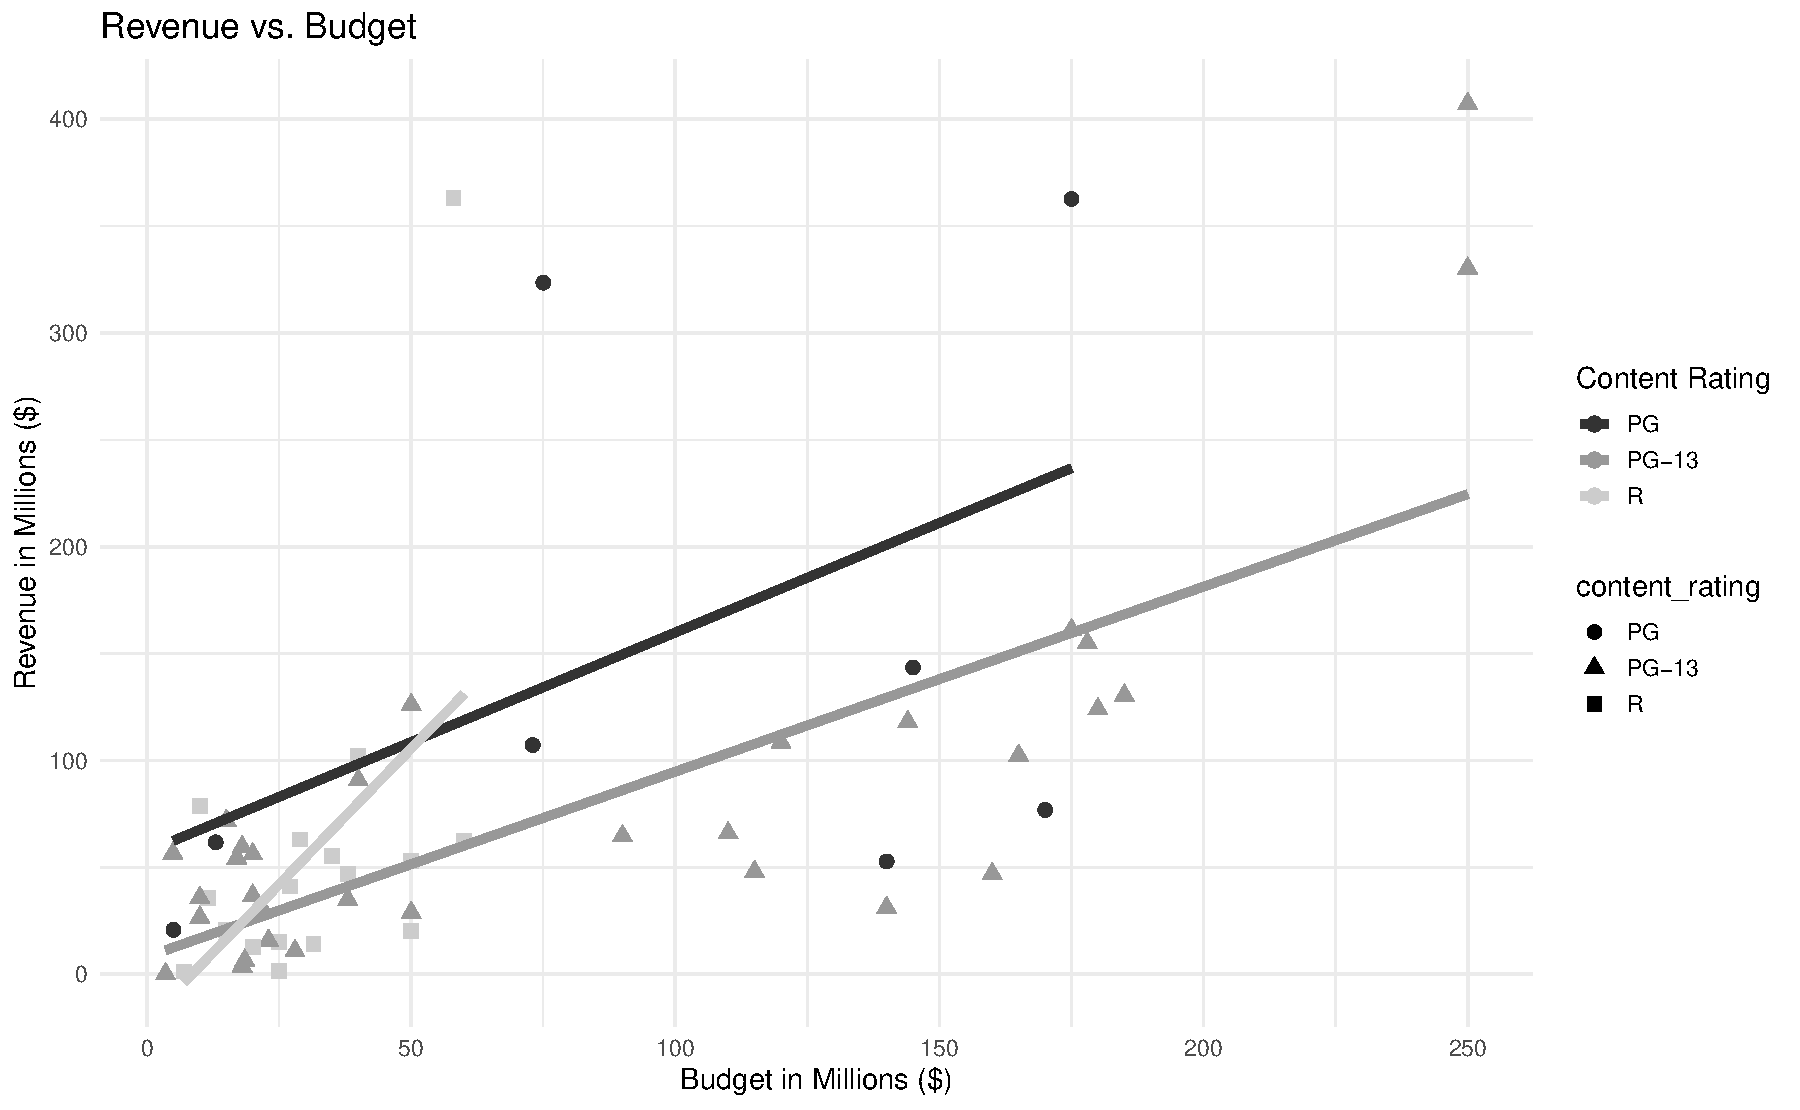
\includegraphics[width=0.7\linewidth]{14-L11-regression-wrapup_files/figure-latex/unnamed-chunk-5-1} \end{center}

\begin{enumerate}
\def\labelenumi{\arabic{enumi}.}
\setcounter{enumi}{5}
\tightlist
\item
  Are the conditions met to use the \(t\)-distribution to approximate the sampling distribution of the standardized statistic? Justify your answer.
\end{enumerate}

\vspace{1.5in}

\hypertarget{ask-a-research-question-7}{%
\subsubsection*{Ask a research question}\label{ask-a-research-question-7}}
\addcontentsline{toc}{subsubsection}{Ask a research question}

\begin{enumerate}
\def\labelenumi{\arabic{enumi}.}
\setcounter{enumi}{6}
\tightlist
\item
  Write out the null and alternative hypotheses in notation to test correlation between the food abundance rating and number of bear complaints.
\end{enumerate}

~~~\(H_O:\)

~~~\(H_A:\)

\hypertarget{use-statistical-inferential-methods-to-draw-inferences-from-the-data-6}{%
\subsubsection*{Use statistical inferential methods to draw inferences from the data}\label{use-statistical-inferential-methods-to-draw-inferences-from-the-data-6}}
\addcontentsline{toc}{subsubsection}{Use statistical inferential methods to draw inferences from the data}

\hypertarget{hypothesis-test-4}{%
\paragraph*{Hypothesis test}\label{hypothesis-test-4}}
\addcontentsline{toc}{paragraph}{Hypothesis test}

Use the \texttt{regression\_test()} function in \texttt{R} (in the \texttt{catstats} package) to simulate the null distribution of sample correlations and compute a p-value. We will need to enter the response variable name and the explanatory variable name for the formula, the data set name (identified above as \texttt{bears}), the statistic for the test, number of repetitions, the sample statistic (value of correlation), and the direction of the alternative hypothesis.

The response variable name is \texttt{Complaints} and the explanatory variable name is \texttt{Food}.

\begin{enumerate}
\def\labelenumi{\arabic{enumi}.}
\setcounter{enumi}{7}
\tightlist
\item
  What inputs should be entered for each of the following to create the simulation to test correlation?
\end{enumerate}

\vspace{.5 mm}

\begin{itemize}
\tightlist
\item
  Direction (\texttt{"greater"}, \texttt{"less"}, or \texttt{"two-sided"}):
\end{itemize}

\vspace{.2in}

\begin{itemize}
\tightlist
\item
  Statistic (choose \texttt{"slope"} or \texttt{"correlation"}):
\end{itemize}

\vspace{.2in}

\begin{itemize}
\tightlist
\item
  As extreme as (enter the value for the sample slope):
\end{itemize}

\vspace{0.2in}

\begin{itemize}
\tightlist
\item
  Number of repetitions:
\end{itemize}

\vspace{.2in}

Using the \texttt{R} script file for this activity, enter your answers for question 8 in place of the \texttt{xx}'s to produce the null distribution with 1000 simulations. Highlight and run lines 1--13 and then lines 44--49.

\begin{Shaded}
\begin{Highlighting}[]
\FunctionTok{regression\_test}\NormalTok{(Complaints }\SpecialCharTok{\textasciitilde{}}\NormalTok{ Food, }\CommentTok{\# response \textasciitilde{} explanatory}
               \AttributeTok{data =}\NormalTok{ bears, }\CommentTok{\# Name of data set}
               \AttributeTok{direction =} \StringTok{"xx"}\NormalTok{, }\CommentTok{\# Sign in alternative ("greater", "less", "two{-}sided")}
               \AttributeTok{statistic =} \StringTok{"xx"}\NormalTok{, }\CommentTok{\# "slope" or "correlation"}
               \AttributeTok{as\_extreme\_as =}\NormalTok{ xx, }\CommentTok{\# Observed slope or correlation}
               \AttributeTok{number\_repetitions =} \DecValTok{1000}\NormalTok{) }\CommentTok{\# Number of simulated samples for null distribution}
       
\end{Highlighting}
\end{Shaded}

\begin{enumerate}
\def\labelenumi{\arabic{enumi}.}
\setcounter{enumi}{8}
\item
  Report the p-value from the \texttt{R} output.
  \vspace{0.3in}
\item
  Interpret the p-value in context of the problem.
  \vspace{0.8in}
\end{enumerate}

\hypertarget{simulation-based-confidence-interval-1}{%
\subsubsection*{Simulation-based confidence interval}\label{simulation-based-confidence-interval-1}}
\addcontentsline{toc}{subsubsection}{Simulation-based confidence interval}

We will use the \texttt{regression\_bootstrap\_CI()} function in \texttt{R} (in the \texttt{catstats} package) to simulate the bootstrap distribution of sample correlations and calculate a confidence interval. Fill in the \texttt{xx}'s in the the provided \texttt{R} script file to find a 90\% confidence interval. Highlight and run lines 52--56.

\begin{Shaded}
\begin{Highlighting}[]
\FunctionTok{regression\_bootstrap\_CI}\NormalTok{(Complaints}\SpecialCharTok{\textasciitilde{}}\NormalTok{Food, }\CommentTok{\# response \textasciitilde{} explanatory}
   \AttributeTok{data =}\NormalTok{ bears, }\CommentTok{\# Name of data set}
   \AttributeTok{confidence\_level =}\NormalTok{ xx, }\CommentTok{\# Confidence level as decimal}
   \AttributeTok{statistic =} \StringTok{"xx"}\NormalTok{, }\CommentTok{\# Slope or correlation}
   \AttributeTok{number\_repetitions =} \DecValTok{1000}\NormalTok{) }\CommentTok{\# Number of simulated samples for bootstrap distribution}
\end{Highlighting}
\end{Shaded}

\begin{enumerate}
\def\labelenumi{\arabic{enumi}.}
\setcounter{enumi}{10}
\item
  Report the bootstrap 90\% confidence interval in interval notation.\\
  \vspace{0.5in}
\item
  Interpret the 90\% confidence interval in context of the problem.
  \vspace{0.8in}
\end{enumerate}

\hypertarget{communicate-the-results-and-answer-the-research-question-6}{%
\subsubsection*{Communicate the results and answer the research question}\label{communicate-the-results-and-answer-the-research-question-6}}
\addcontentsline{toc}{subsubsection}{Communicate the results and answer the research question}

\begin{enumerate}
\def\labelenumi{\arabic{enumi}.}
\setcounter{enumi}{12}
\tightlist
\item
  Based on the p-value, write a conclusion in context of the problem.
\end{enumerate}

\vspace{.8in}

\begin{enumerate}
\def\labelenumi{\arabic{enumi}.}
\setcounter{enumi}{13}
\item
  Using a significance level of 0.1, what decision would you make?
  \vspace{0.2in}
\item
  What type of error is possible?
  \vspace{0.3in}
\item
  Write this error in context of the problem.
  \vspace{0.8in}
\item
  Write a paragraph summarizing the results of the study as if you are reporting these results in your local newspaper. Be sure to describe:
\end{enumerate}

\begin{itemize}
\item
  Summary statistic
\item
  Test statistic and interpretation
\item
  P-value and interpretation
\item
  Confidence interval and interpretation
\item
  Conclusion (written to answer the research question)
\item
  Scope of inference
\end{itemize}

\vspace{3in}

\begin{Shaded}
\begin{Highlighting}[]
\NormalTok{bears }\SpecialCharTok{\%\textgreater{}\%}
  \FunctionTok{ggplot}\NormalTok{(}\FunctionTok{aes}\NormalTok{(}\AttributeTok{x =}\NormalTok{ Food, }\AttributeTok{y =}\NormalTok{ Complaints, }\AttributeTok{color=}\NormalTok{Pop\_Level))}\SpecialCharTok{+}  \CommentTok{\# Specify variables}
  \FunctionTok{geom\_point}\NormalTok{(}\FunctionTok{aes}\NormalTok{(}\AttributeTok{shape =}\NormalTok{ Pop\_Level), }\AttributeTok{size =} \DecValTok{3}\NormalTok{) }\SpecialCharTok{+}  \CommentTok{\# Add scatterplot of points}
  \FunctionTok{labs}\NormalTok{(}\AttributeTok{x =} \StringTok{"flipper length (mm)"}\NormalTok{,  }\CommentTok{\# Label x{-}axis}
       \AttributeTok{y =} \StringTok{"body mass (g)"}\NormalTok{,  }\CommentTok{\# Label y{-}axis}
       \AttributeTok{color =} \StringTok{"species"}\NormalTok{,}
       \AttributeTok{title =} \StringTok{"TITLE"}\NormalTok{) }\SpecialCharTok{+} \CommentTok{\# Be sure to tile your plots}
  \FunctionTok{geom\_smooth}\NormalTok{(}\AttributeTok{method =} \StringTok{"lm"}\NormalTok{, }\AttributeTok{se =} \ConstantTok{FALSE}\NormalTok{)  }\CommentTok{\# Add regression line}
\end{Highlighting}
\end{Shaded}

\begin{center}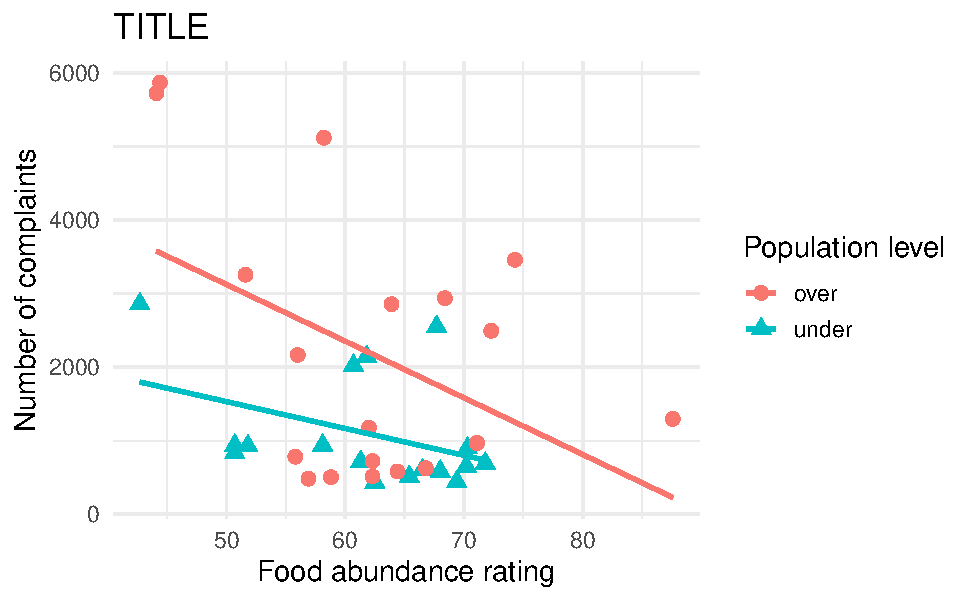
\includegraphics[width=0.6\linewidth]{14-L11-regression-wrapup_files/figure-latex/unnamed-chunk-8-1} \end{center}

\hypertarget{semester-review}{%
\chapter{Semester Review}\label{semester-review}}

\setstretch{1}

\hypertarget{data-exploration-concussions}{%
\section{Data Exploration: Concussions}\label{data-exploration-concussions}}

\hypertarget{learning-objectives-23}{%
\subsection{Learning objectives}\label{learning-objectives-23}}

\begin{enumerate}
\def\labelenumi{\arabic{enumi}.}
\item
  Read research articles and
\item
  Evaluate scope of inference for studies.
\end{enumerate}

\hypertarget{articles-on-concussions.}{%
\subsection*{Articles on Concussions.}\label{articles-on-concussions.}}
\addcontentsline{toc}{subsection}{Articles on Concussions.}

\textbf{Read through the following abstracts before class and be prepared to discuss the following questions in your groups.}

\begin{enumerate}
\def\labelenumi{(\alph{enumi})}
\item
  The questions researchers wanted to answer.
\item
  Who/what were the subjects?
\item
  Were treatments applied at random?
\end{enumerate}

\begin{enumerate}
\def\labelenumi{\arabic{enumi}.}
\tightlist
\item
  Petraglia AL, Plog BA, Dayawansa S, Chen M, Dashnaw ML, Czerniecka K, Walker CT, Viterise T, Hyrien O, Iliff JJ, Deane R, Nedergaard M, Huang JH. (2014). \emph{The spectrum of neurobehavioral consequences after repetitive mild traumatic brain injury: a novel mouse model of chronic traumatic encephalopathy.}
  J Neurotrauma Jul 1; 31(13):1211-24.
\end{enumerate}

\url{http://www.ncbi.nlm.nih.gov/pubmed/24766454}

Abstract

There has been an increased focus on the neurological consequences of repetitive mild traumatic brain injury (TBI), particularly neurodegenerative syndromes, such as chronic traumatic encephalopathy (CTE); however, no animal model exists that captures the behavioral spectrum of this phenomenon. We sought to develop an animal model of CTE. Our novel model is a modification and fusion of two of the most popular models of TBI and allows for controlled closed-head impacts to unanesthetized mice. Two-hundred and eighty 12-week-old mice were divided into control, single mild TBI (mTBI), and repetitive mTBI groups. Repetitive mTBI mice received six concussive impacts daily for 7 days. Behavior was assessed at various time points. Neurological Severity Score (NSS) was computed and vestibulomotor function tested with the wire grip test (WGT). Cognitive function was assessed with the Morris water maze (MWM), anxiety/risk-taking behavior with the elevated plus maze, and depression-like behavior with the forced swim/tail suspension tests. Sleep electroencephalogram/electromyography studies were performed at 1 month. NSS was elevated, compared to controls, in both TBI groups and improved over time. Repetitive mTBI mice demonstrated transient vestibulomotor deficits on WGT. Repetitive mTBI mice also demonstrated deficits in MWM testing. Both mTBI groups demonstrated increased anxiety at 2 weeks, but repetitive mTBI mice developed increased risk-taking behaviors at 1 month that persist at 6 months. Repetitive mTBI mice exhibit depression-like behavior at 1 month. Both groups demonstrate sleep disturbances. We describe the neurological consequenses of repetitive mTBI in a novel mouse model, which resemble several of the neuropsychiatric behaviors observed clinically in patients sustaining repetitive mild head injury.

\begin{enumerate}
\def\labelenumi{\arabic{enumi}.}
\setcounter{enumi}{1}
\tightlist
\item
  Lin, Ramadan, Stern, Box, Nowinski, Ross, Mountford. (2015). \emph{Changes in the neurochemistry of athletes with repetitive brain trauma: preliminary results using localized correlated spectroscopy.} Alzheimers Research \& Therapy.
  2015 Mar 15;7(1):13
\end{enumerate}

\url{http://www.ncbi.nlm.nih.gov/pubmed/25780390}

Abstract
INTRODUCTION:

The goal was to identify which neurochemicals differ in professional athletes with repetitive brain trauma (RBT) when compared to healthy controls using a relatively new technology, in vivo Localized COrrelated SpectroscopY (L-COSY).

METHODS:

To achieve this, L-COSY was used to examine five former professional male athletes with 11 to 28 years of exposure to contact sports. Each athlete who had had multiple symptomatic concussions and repetitive sub concussive trauma during their career was assessed by an experienced neuropsychologist. All athletes had clinical symptoms including headaches, memory loss, confusion, impaired judgment, impulse control problems, aggression, and depression. Five healthy men, age and weight matched to the athlete cohort and with no history of brain trauma, were recruited as controls. Data were collected from the posterior cingulate gyrus using a 3 T clinical magnetic resonance scanner equipped with a 32 channel head coil.

RESULTS:

The variation of the method was calculated by repeated examination of a healthy control and phantom and found to be 10\% and 5\%, respectively, or less. The L-COSY measured large and statistically significant differences (P \textless=0.05), between healthy controls and those athletes with RBT. Men with RBT showed higher levels of glutamine/glutamate (31\%), choline (65\%), fucosylated molecules (60\%) and phenylalanine (46\%). The results were evaluated and the sample size of five found to achieve a significance level P=0.05. Differences in N-acetyl aspartate and myoinositol between RBT and controls were small and were not statistically significance.

CONCLUSIONS:

A study of a small cohort of professional athletes, with a history of RBT and symptoms of chronic traumatic encephalopathy when compared with healthy controls using 2D L-COSY, showed elevations in brain glutamate/glutamine and choline as recorded previously for early traumatic brain injury. For the first time increases in phenylalanine and fucose are recorded in the brains of athletes with RBT. Larger studies utilizing the L-COSY method may over an in-life method of diagnosis and personalized approach for monitoring the acute effects of mild traumatic brain injury and the chronic effects of RBT.

\begin{enumerate}
\def\labelenumi{\arabic{enumi}.}
\setcounter{enumi}{2}
\tightlist
\item
  Here's a quote from a news report in 2013:
  ``We need to figure out what's making some people more vulnerable than others,'' says Michelle Mielke, an Alzheimer's researcher at the Mayo Clinic who led the study. It was published online Thursday in the journal Neurology. Just because you have a head trauma doesn't mean you're going to develop memory problems or significant amyloid levels," Mielke told Shots. And it doesn't
  mean you're going to get Alzheimer's. ``But it does suggest to us that there's a mechanism with head trauma that does increase your risk.''
\end{enumerate}

Mielke and her colleagues did PET scans on 589 people who are participating in a long-term study of aging and memory. That's a lot of people for a brain imaging study, which makes it more likely that the findings are accurate.

\url{http://www.npr.org/blogs/health/2013/12/27/257552665/concussions-may-increase-alzheimers-risk-but-only-for-some}

\hypertarget{applying-what-weve-learned}{%
\subsection*{Applying What We've Learned}\label{applying-what-weve-learned}}
\addcontentsline{toc}{subsection}{Applying What We've Learned}

Some have argued that blows to the head - for instance on the high school football field - are getting too much attention. They point out that of many kids taking similar hits, only a few show lasting decrease in cognitive abilities, and suggest that the effects are as much due to genetics as to the blow to the head.

\begin{enumerate}
\def\labelenumi{\arabic{enumi}.}
\tightlist
\item
  Your group is asked to design a study to determine how large a risk the ``hits''
  taken by high school athletes are to their future cognitive abilities. Write down
  a plan for your study. Include:
\end{enumerate}

\begin{itemize}
\item
  Who will your subjects be? How will you find them? How many will you need?
\item
  What will you measure? (Brain scans like MRI? Cognitive tests of memory and reasoning? Some measure of emotional states like anger?) Include the timing of measurements.
\item
  Will your study be observational or an experiment?
\item
  Is your study ethical in its treatment of subjects?
\end{itemize}

\vspace{1in}

\begin{enumerate}
\def\labelenumi{\arabic{enumi}.}
\setcounter{enumi}{1}
\tightlist
\item
  Trade papers with another group and read their study over carefully. Address the bullet points above. Provide suggestions as to what might be improved.
\end{enumerate}

\begin{itemize}
\tightlist
\item
  Subjects?
\end{itemize}

\vspace{0.5in}

\begin{itemize}
\tightlist
\item
  Measurements?
\end{itemize}

\vspace{0.5in}

\begin{itemize}
\tightlist
\item
  Observational? Experiment?
\end{itemize}

\vspace{0.5in}

\begin{itemize}
\tightlist
\item
  Ethical issues?
\end{itemize}

\vspace{0.5in}

\begin{enumerate}
\def\labelenumi{\arabic{enumi}.}
\setcounter{enumi}{2}
\tightlist
\item
  For today's class you read the abstract from this article.
\end{enumerate}

Petraglia AL, Plog BA, Dayawansa S, Chen M, Dashnaw ML, Czerniecka K, Walker CT, Viterise T, Hyrien O, Iliff JJ, Deane R, Nedergaard M, Huang JH. (2014). \emph{The spectrum of neurobehavioral consequences after repetitive mild traumatic brain injury: a novel mouse model of chronic traumatic encephalopathy.} J Neurotrauma Jul 1; 31(13):1211-24.

\url{http://www.ncbi.nlm.nih.gov/pubmed/24766454}

\begin{enumerate}
\def\labelenumi{\alph{enumi})}
\tightlist
\item
  What are the advantages of this study design?
\end{enumerate}

\vspace{0.5in}

\begin{enumerate}
\def\labelenumi{\alph{enumi})}
\setcounter{enumi}{1}
\tightlist
\item
  Disadvantages?
\end{enumerate}

\vspace{0.5in}

\begin{enumerate}
\def\labelenumi{\alph{enumi})}
\setcounter{enumi}{2}
\tightlist
\item
  Does the design allow us to make causal inferences? Explain.
\end{enumerate}

\vspace{0.5in}

\begin{enumerate}
\def\labelenumi{\alph{enumi})}
\setcounter{enumi}{3}
\tightlist
\item
  Inferences to high school students? Explain.
\end{enumerate}

\vspace{0.5in}

\begin{enumerate}
\def\labelenumi{\arabic{enumi}.}
\setcounter{enumi}{3}
\tightlist
\item
  And you read this abstract:
  Lin, Ramadan, Stern, Box, Nowinski, Ross, Mountford. (2015). \emph{Changes in the neurochemistry of athletes with repetitive brain trauma: preliminary results using localized correlated spectroscopy.} Alzheimers Research \& Therapy.
  2015 Mar 15;7(1):13
\end{enumerate}

\url{http://www.ncbi.nlm.nih.gov/pubmed/25780390}

\begin{enumerate}
\def\labelenumi{\alph{enumi})}
\tightlist
\item
  What are the advantages of this study design?
\end{enumerate}

\vspace{0.5in}

\begin{enumerate}
\def\labelenumi{\alph{enumi})}
\setcounter{enumi}{1}
\tightlist
\item
  Disadvantages?
\end{enumerate}

\vspace{0.5in}

\begin{enumerate}
\def\labelenumi{\alph{enumi})}
\setcounter{enumi}{2}
\tightlist
\item
  Does the design allow us to make causal inferences? Explain.
\end{enumerate}

\vspace{0.5in}

\begin{enumerate}
\def\labelenumi{\alph{enumi})}
\setcounter{enumi}{3}
\tightlist
\item
  Inferences to high school students? Explain.
\end{enumerate}

\vspace{0.5in}

\begin{enumerate}
\def\labelenumi{\arabic{enumi}.}
\setcounter{enumi}{4}
\tightlist
\item
  Here's a quote from a news report in 2013:
  ``Mielke and her colleagues did PET scans on 589 people who are participating in a long-term study of aging and memory. That's a lot of people for a brain imaging study, which makes it more likely that the findings are accurate.''
\end{enumerate}

\url{http://www.npr.org/blogs/health/2013/12/27/257552665/concussions-may-increase-alzheimers-risk-but-only-for-some}

Explain the last sentence. In what sense does a large sample increase accuracy?

\vspace{1in}

\hypertarget{take-home-messages-22}{%
\subsection{Take Home Messages}\label{take-home-messages-22}}

\begin{enumerate}
\def\labelenumi{\arabic{enumi}.}
\item
  In reading a research article, carefully read what they say about selection of subjects (or units of study) so we know how far we can extend our inference.
\item
  Similarly, evaluate the assignment of any treatments (at random, we hope) so that we know if causal inference is appropriate.
\item
  In designing a study, we'd like to get a large sample, but expense might prevent that.
\item
  You might see names of tests we've not covered, but the idea of a p-value is the same for any test, and the null hypothesis is generally ``No change,'' or ``No effect.''
\end{enumerate}

\hypertarget{additional-notes-21}{%
\subsection{Additional notes}\label{additional-notes-21}}

Use this space to summarize your thoughts and take additional notes on today's activity and material covered.

\newpage

\hypertarget{final-exam-review}{%
\section{Final Exam Review}\label{final-exam-review}}

\setstretch{1}

Use the provided data set from the Islands (ExamReviewData.csv) and the Exam 2 Review \texttt{R} script file to answer the following questions. Each adult (\textgreater21) islander was selected at random from all the adult islanders.

\begin{longtable}[]{@{}
  >{\raggedright\arraybackslash}p{(\columnwidth - 2\tabcolsep) * \real{0.24}}
  >{\raggedright\arraybackslash}p{(\columnwidth - 2\tabcolsep) * \real{0.76}}@{}}
\toprule
\textbf{Variable} & \textbf{Description} \\
\midrule
\endhead
\texttt{Island} & Name of Island that the Islander resides on \\
\texttt{City} & Name of City in which the Islander resides \\
\texttt{Population} & Population of the City \\
\texttt{Name} & Name of Islander \\
\texttt{Consent} & Whether the Islander consented to be in the study \\
\texttt{Gender} & Gender of Islander (M = male, F = Female) \\
\texttt{Age} & Age of Islander \\
\texttt{Married} & Marital status of Islander \\
\texttt{Smoking\_Status} & Whether the Islander is a current smoker \\
\texttt{Children} & Whether the Islander has children \\
\texttt{weight\_kg} & Weight measured in kg \\
\texttt{height\_cm} & Height measured in cm \\
\texttt{respitory\_rate} & Breaths per minute \\
\texttt{Type\_of\_Music} & Music type (Classical or Heavy Medal) Islander was randomly assigned to listen to \\
\texttt{Before\_PuzzleCube} & Time to complete puzzle cube (minutes) before listening to assigned music \\
\texttt{After\_PuzzleCube} & Time to complete puzzle cube (minutes) after listening to assigned music \\
\texttt{Diff\_PuzzleCube} & Difference in time to complete puzzle cube (minutes) for Before - After listening to assigned music \\
\texttt{Education\_Level} & Highest level of education completed (note: missing data depicted by missing) \\
\texttt{Balance\_Test} & Time balanced measured in seconds with eyes closed \\
\texttt{Blood\_Glucose\_before} & Level of blood glucose (mg/dL) before consuming assigned drink \\
\texttt{Heart\_Rate\_before} & Heart rate (bpm) before consuming assigned drink \\
\texttt{Type\_of\_Drink} & Type of drink (EnergyDrink or Cola) Islander was randomly assigned to drink \\
\texttt{Heart\_Rate\_after} & Heart rate (bpm) after consuming assigned drink \\
\texttt{Blood\_Glucose\_after} & Level of blood glucose (mg/dL) after consuming assigned drink \\
\texttt{Diff\_Heart\_Rate} & Difference in heart rate (bpm) for Before - After consuming assigned drink \\
\texttt{Diff\_Blood\_Glucose} & Difference in blood glucose (mg/dL) for Before - After consuming assigned drink \\
\bottomrule
\end{longtable}

\begin{enumerate}
\def\labelenumi{\arabic{enumi}.}
\tightlist
\item
  Write a research question involving a paired quantitative variable that can be answered using the data set.
\end{enumerate}

\vspace{0.8in}

\begin{enumerate}
\def\labelenumi{\arabic{enumi}.}
\setcounter{enumi}{1}
\tightlist
\item
  Use the provided Final Exam Review \texttt{R} script file and analyze this research question.
\end{enumerate}

\rgi Parameter of Interest:

\vspace{0.3in}

\rgi Null Hypothesis:

\rgi \rgi Notation:

\vspace{0.3in}

\rgi \rgi Words:

\vspace{0.5in}

\rgi Alternative Hypothesis:

\rgi \rgi Notation:

\vspace{0.3in}

\rgi \rgi Words:

\vspace{0.5in}

\rgi Statistic:

\vspace{0.3in}

\rgi Conditions:

\rgi \rgi Independence:

\vspace{0.8in}

\rgi \rgi Normality:

\vspace{0.8in}

\rgi Simulation P-value:

\vspace{0.3in}

\rgi \rgi Interpretation:

\vspace{0.8in}

\rgi \rgi Conclusion:

\vspace{0.8in}

\rgi \rgi Decision:

\vspace{0.3in}

\rgi Simulation Confidence Interval:

\vspace{0.3in}

\rgi \rgi Interpretation:

\vspace{0.8in}

\rgi Standardized Statistic:

\vspace{0.3in}

\rgi \rgi Interpretation:

\vspace{0.8in}

\rgi Theory-based p-value:

\vspace{0.3in}

\rgi Theory-based Confidence Interval:

\vspace{0.3in}

\rgi Does the theory-based p-value and CI match those found using simulation methods?

\vspace{0.8in}

\rgi What is the scope of inference for this study?

\vspace{0.8in}

\begin{enumerate}
\def\labelenumi{\arabic{enumi}.}
\setcounter{enumi}{2}
\tightlist
\item
  Write a research question involving a single categorical variable and a single quantitative variable that can be answered using the data set.
\end{enumerate}

\vspace{0.8in}

\begin{enumerate}
\def\labelenumi{\arabic{enumi}.}
\setcounter{enumi}{3}
\tightlist
\item
  Use the provided Final Exam Review \texttt{R} script file and analyze this research question.
\end{enumerate}

\rgi Parameter of Interest:

\vspace{0.3in}

\rgi Null Hypothesis:

\rgi \rgi Notation:

\vspace{0.3in}

\rgi \rgi Words:

\vspace{0.5in}

\rgi Alternative Hypothesis:

\rgi \rgi Notation:

\vspace{0.3in}

\rgi \rgi Words:

\vspace{0.5in}

\rgi Statistic:

\vspace{0.3in}

\rgi Conditions:

\rgi \rgi Independence:

\vspace{0.8in}

\rgi \rgi Normality:

\vspace{0.8in}

\rgi Simulation P-value:

\vspace{0.3in}

\rgi \rgi Interpretation:

\vspace{0.8in}

\rgi \rgi Conclusion:

\vspace{0.8in}

\rgi \rgi Decision:

\vspace{0.3in}

\rgi Simulation Confidence Interval:

\vspace{0.3in}

\rgi \rgi Interpretation:

\vspace{0.8in}

\rgi Standardized Statistic:

\vspace{0.3in}

\rgi \rgi Interpretation:

\vspace{0.8in}

\rgi Theory-based p-value:

\vspace{0.3in}

\rgi Theory-based Confidence Interval:

\vspace{0.3in}

\rgi Does the theory-based p-value and CI match those found using simulation methods?

\vspace{0.8in}

\rgi What is the scope of inference for this study?

\vspace{0.8in}

\begin{enumerate}
\def\labelenumi{\arabic{enumi}.}
\setcounter{enumi}{4}
\tightlist
\item
  Write a research question involving a two quantitative variables that can be answered using the data set.
\end{enumerate}

\vspace{0.8in}

\begin{enumerate}
\def\labelenumi{\arabic{enumi}.}
\setcounter{enumi}{3}
\tightlist
\item
  Use the provided Final Exam Review \texttt{R} script file and analyze this research question.
\end{enumerate}

\rgi Parameter of Interest:

\vspace{0.3in}

\rgi Null Hypothesis:

\rgi \rgi Notation:

\vspace{0.3in}

\rgi \rgi Words:

\vspace{0.5in}

\rgi Alternative Hypothesis:

\rgi \rgi Notation:

\vspace{0.3in}

\rgi \rgi Words:

\vspace{0.5in}

\rgi Statistic:

\vspace{0.3in}

\rgi Conditions:

\rgi \rgi Independence:

\vspace{0.8in}

\rgi \rgi Normality:

\vspace{0.8in}

\rgi Simulation P-value:

\vspace{0.3in}

\rgi \rgi Interpretation:

\vspace{0.8in}

\rgi \rgi Conclusion:

\vspace{0.8in}

\rgi \rgi Decision:

\vspace{0.3in}

\rgi Simulation Confidence Interval:

\vspace{0.3in}

\rgi \rgi Interpretation:

\vspace{0.8in}

\rgi Standardized Statistic:

\vspace{0.3in}

\rgi \rgi Interpretation:

\vspace{0.8in}

\rgi Theory-based p-value:

\vspace{0.3in}

\rgi Theory-based Confidence Interval:

\vspace{0.3in}

\rgi Does the theory-based p-value and CI match those found using simulation methods?

\vspace{0.8in}

\rgi What is the scope of inference for this study?

\vspace{0.8in}

\newpage

\hypertarget{refs}{}
\begin{CSLReferences}{1}{0}
\leavevmode\vadjust pre{\hypertarget{ref-banerjee2018}{}}%
Banerjee, S. 2018. {``Linear Regression: Moneyball -- Part 1.''} \emph{Medium}. \url{https://towardsdatascience.com/linear-regression-moneyball-part-1-b93b3b9f5b53}.

\leavevmode\vadjust pre{\hypertarget{ref-imdb}{}}%
{``{IMDb} Movies Extensive Dataset.''} n.d. \url{https://kaggle.com/stefanoleone992/imdb-extensive-dataset}.

\leavevmode\vadjust pre{\hypertarget{ref-johnson2006}{}}%
Johnson, C. M.., and J. E. Memmott. 2006. {``Examination of Relationships Between Participation in School Music Programs of Differing Quality and Standardized Test Results.''} \emph{Journal of Research in Music Education} 54 (4): 293--307. \url{https://doi.org/10.1177/002242940605400403}.

\leavevmode\vadjust pre{\hypertarget{ref-moneyball}{}}%
{``Moneyball Dataset.''} n.d. \url{https://kaggle.com/wduckett/moneyball-mlb-stats-19622012}.

\leavevmode\vadjust pre{\hypertarget{ref-weather}{}}%
National Weather Service Corporate Image Web Team. n.d. {``National Weather Service -- {NWS} Billings.''} \url{https://w2.weather.gov/climate/xmacis.php?wfo=byz}.

\leavevmode\vadjust pre{\hypertarget{ref-ohair2017}{}}%
O'Hair, A. 2017. {``Video 4: Using the Model to Make Predictions.''} {MIT}: {MIT Open Courseware}. \url{https://ocw.mit.edu/courses/sloan-school-of-management/15-071-the-analytics-edge-spring-2017/linear-regression/moneyball-the-power-of-sports-analytics/video-4-using-the-models-to-make-predictions/}.

\leavevmode\vadjust pre{\hypertarget{ref-quinn1999}{}}%
Quinn, G. E., C. H. Shin, M. G. Maguire, and R. A. Stone. 1999. {``Myopia and Ambient Lighting at Night.''} \emph{Nature} 399 (6732): 113--14. \url{https://doi.org/10.1038/20094}.

\leavevmode\vadjust pre{\hypertarget{ref-ramachandran2007}{}}%
Ramachandran, V. 2007. {``3 Clues to Understanding Your Brain.''} \url{https://www.ted.com/talks/vs_ramachandran_3_clues_to_understanding_your_brain}.

\leavevmode\vadjust pre{\hypertarget{ref-richardson2019}{}}%
Richardson, T., and R. T. Gilman. 2019. {``Left-Handedness Is Associated with Greater Fighting Success in Humans.''} \emph{Scientific Reports} 9 (1): 15402. \url{https://doi.org/10.1038/s41598-019-51975-3}.

\leavevmode\vadjust pre{\hypertarget{ref-stewart2014}{}}%
Stewart, E. H., B. Davis, B. L. Clemans-Taylor, B. Littenberg, C. A. Estrada, and R. M. Centor. 2014. {``Rapid Antigen Group a Streptococcus Test to Diagnose Pharyngitis: A Systematic Review and Meta-Analysis''} 9 (11). \url{https://doi.org/10.1371/journal.pone.0111727}.

\leavevmode\vadjust pre{\hypertarget{ref-sulheim2017}{}}%
Sulheim, S., A. Ekeland, I. Holme, and R. Bahr. 2017. {``Helmet Use and Risk of Head Injuries in Alpine Skiers and Snowboarders: Changes After an Interval of One Decade''} 51 (1): 44--50. \url{https://doi.org/10.1136/bjsports-2015-095798}.

\leavevmode\vadjust pre{\hypertarget{ref-usepa2020}{}}%
US Environmental Protection Agency. n.d. {``Air Data -- Daily Air Quality Tracker.''} \url{https://www.epa.gov/outdoor-air-quality-data/air-data-daily-air-quality-tracker}.

\end{CSLReferences}

\end{document}
